%
\documentclass[
  notoc % Suppress Tufte style table of contents.
]{tufte-book}

% Required Tufte packages.
\usepackage{changepage} % or changepage
\usepackage{fancyhdr}
\usepackage{fontenc}
\usepackage{geometry}
\usepackage{hyperref}
\usepackage{natbib}
\usepackage{bibentry}
\usepackage{optparams}
\usepackage{paralist}
\usepackage{placeins}
\usepackage{ragged2e}
\usepackage{setspace}
\usepackage{textcase}
\usepackage{textcomp}
\usepackage{titlesec}
\usepackage{titletoc}
\usepackage{xcolor}
\usepackage{xifthen}

\geometry{paperheight=10in,paperwidth=7in,marginparwidth=30mm,marginparsep=2mm,bindingoffset=10mm,top=10mm,inner=8mm,outer=8mm,bottom=16mm,includehead,includemp}

% Tufte vs. Pandoc workaround.
% Issue: https://github.com/Tufte-LaTeX/tufte-latex/issues/64.
\renewcommand\allcapsspacing[1]{{\addfontfeature{LetterSpace=15}#1}}
\renewcommand\smallcapsspacing[1]{{\addfontfeature{LetterSpace=10}#1}}

% \setmainfont{TeX Gyre Pagella}
\usepackage[utf8]{inputenc}
\usepackage[T1]{fontenc}
\setmainfont{texgyrepagella}[
  Extension = .otf,
  UprightFont = *-regular,
  BoldFont = *-bold,
  ItalicFont = *-italic,
  BoldItalicFont = *-bolditalic,
]

\newfontfamily\JuliaMono{JuliaMono}[
  UprightFont = *-Regular,
  BoldFont = *-Bold
]
\newfontface\JuliaMonoRegular{JuliaMono-Regular}
\newfontface\JuliaMonoBold{JuliaMono-Bold}

\setmonofont{JuliaMono-Medium}[
  Contextuals=Alternate,
  Ligatures=NoCommon
]


\usepackage{graphicx}
\makeatletter
\def\maxwidth{\ifdim\Gin@nat@width>\linewidth\linewidth\else\Gin@nat@width\fi}
\def\maxheight{\ifdim\Gin@nat@height>\textheight\textheight\else\Gin@nat@height\fi}
\makeatother
% Scale images if necessary, so that they will not overflow the page
% margins by default, and it is still possible to overwrite the defaults
% using explicit options in \includegraphics[width, height, ...]{}
\setkeys{Gin}{width=\maxwidth,height=\maxheight,keepaspectratio}
\DeclareRobustCommand{\href}[2]{#2\footnote{\url{#1}}}

\usepackage{float}
\floatplacement{figure}{H}

% Listings Julia syntax definition.
\input{/home/runner/.julia/packages/Books/C7CMR/defaults/julia_listings.tex}

% Unicode support.
\input{/home/runner/.julia/packages/Books/C7CMR/defaults/julia_listings_unicode.tex}

% Used by Pandoc.
\providecommand{\tightlist}{%
  \setlength{\itemsep}{0pt}\setlength{\parskip}{0pt}
}
\newcommand{\passthrough}[1]{#1}

\usepackage{longtable}
\usepackage{booktabs}
\usepackage{array}

% Source: Wandmalfarbe/pandoc-latex-template.
\newlength{\cslhangindent}
\setlength{\cslhangindent}{1.5em}
\newlength{\csllabelwidth}
\setlength{\csllabelwidth}{3em}
\newenvironment{CSLReferences}[2] % #1 hanging-ident, #2 entry spacing
 {% don't indent paragraphs
  \setlength{\parindent}{0pt}
  % turn on hanging indent if param 1 is 1
  \ifodd #1 \everypar{\setlength{\hangindent}{\cslhangindent}}\ignorespaces\fi
  % set entry spacing
  \ifnum #2 > 0
  \setlength{\parskip}{#2\baselineskip}
  \fi
 }%
 {}
\usepackage{calc}
\newcommand{\CSLBlock}[1]{#1\hfill\break}
\newcommand{\CSLLeftMargin}[1]{\parbox[t]{\csllabelwidth}{#1}}
\newcommand{\CSLRightInline}[1]{\parbox[t]{\linewidth - \csllabelwidth}{#1}\break}
\newcommand{\CSLIndent}[1]{\hspace{\cslhangindent}#1}

\definecolor{linkblue}{HTML}{117af2}
\usepackage{hyperref}
\hypersetup{
  colorlinks,
  citecolor=linkblue,
  linkcolor=linkblue,
  urlcolor=linkblue,
  linktoc=page, % Avoid Table of Contents being nearly completely blue.
  pdftitle={Julia Data Science},
  pdfauthor={Jose Storopoli; Rik Huijzer; Lazaro Alonso},
  pdflang={en-US},
  breaklinks=true,
  pdfcreator={LaTeX via Pandoc}%
}
\urlstyle{same} % disable monospaced font for URLs

\title{Julia Data Science}
\author{\noindent{Jose Storopoli}\\[3mm] \noindent{Rik
Huijzer}\\[3mm] \noindent{Lazaro Alonso}\\[3mm] }
\date{}

% Re-enable section numbering which was disabled by tufte.
\setcounter{secnumdepth}{2}

% Fix captions for longtable.
% Thanks to David Carlisle at https://tex.stackexchange.com/a/183344/92217.
\makeatletter
\def\LT@makecaption#1#2#3{%
  \noalign{\smash{\hbox{\kern\textwidth\rlap{\kern\marginparsep
  \parbox[t]{\marginparwidth}{\vspace{12pt}%
\@tufte@caption@font \@tufte@caption@justification \noindent
   #1{#2: }\ignorespaces #3}}}}}}
\makeatother

% Doesn't seem to do anything.
\usepackage{float}
\floatplacement{figure}{H}
\floatplacement{table}{H}

% Reduce large spacing around sections.
\titlespacing*{\chapter}{0pt}{5pt}{20pt}
\titlespacing*{\section}{0pt}{2.5ex plus 1ex minus .2ex}{1.3ex plus .2ex}
\titlespacing*{\subsection}{0pt}{1.75ex plus 1ex minus .2ex}{1.0ex plus.2ex}

\titleformat{\chapter}%
  [hang]% shape
  {\normalfont\huge\itshape}% format applied to label+text
  {\huge\thechapter}% label
  {1em}% horizontal separation between label and title body
  {}% before the title body
  []% after the title body

% Reduce spacing in table of contents.
\usepackage{etoolbox}
\makeatletter
\pretocmd{\chapter}{\addtocontents{toc}{\protect\addvspace{-3\p@}}}{}{}
\pretocmd{\section}{\addtocontents{toc}{\protect\addvspace{-4\p@}}}{}{}
\pretocmd{\subsection}{\addtocontents{toc}{\protect\addvspace{-5\p@}}}{}{}
\makeatother

% Long texts are harder to read than tables.
% Therefore, we can reduce the font size of the table.
\AtBeginEnvironment{longtable}{\footnotesize}

% Some space between paragraphs is necessary because code blocks can output single line paragraphs.
\setlength\parskip{1em plus 0.1em minus 0.2em}

% For justified text.
\usepackage{ragged2e}

% tufte-book disables subsubsections by default.
% Got this definition back via `\show\subsubsection`.
\makeatletter
\renewcommand\subsubsection{%
\@startsection{subsubsection}{3}{\z@ }{-3.25ex\@plus -1ex \@minus -.2ex}{1.5ex \@plus .2ex}{\normalfont \normalsize \bfseries }
}
\makeatother

\usepackage{amsfonts}
\usepackage{amssymb}
\usepackage{amsmath}
\usepackage{unicode-math}

% URL line breaks.
\usepackage{xurl}

% Probably doesn't hurt.
\usepackage{marginfix}


\begin{document}

\makeatletter
\thispagestyle{empty}
\vfill
{\Huge\bf
\noindent
\@title
}\\[1in]
{\Large
\noindent
\@author
}
\makeatother

\makeatletter
\newpage
\thispagestyle{empty}
\vfill
{\noindent
\begin{tabular}{l} Jose Storopoli\\ Universidade Nove de Julho - UNINOVE\\ Brazil\\ \\ Rik Huijzer\\ University of Groningen\\ the Netherlands\\ \\ Lazaro Alonso\\ Max Planck Institute for Biogeochemistry\\ Germany \end{tabular}
}
\vfill
{\small
First edition published 2021

\url{https://juliadatascience.io}

ISBN: 9798489859165

2022-12-11

Creative Commons Attribution-NonCommercial-ShareAlike 4.0 International
}
\makeatother


% Don't remove this or authors will show up in header of every page.
\frontmatter
\mainmatter

\setcounter{tocdepth}{1}
\tableofcontents

% Justify text.
\justifying

% parindent seems to be set from within another class too.
% it is really not useful here because it will also indent lines directly after
% code blocks. Which most of the times not useful.
\setlength{\parindent}{0pt}

\hypertarget{sec:preface}{%
\chapter{Prefácio}\label{sec:preface}}

Existem várias linguagens de programação e cada uma delas tem seus
pontos fortes e fracos. Algumas linguagens são mais rápidas, mas
bastante verbosas. Outras linguagens são fáceis de codificar, mas são
lentas. Isso é conhecido como o problema das \emph{duas linguagens} e
Julia busca eliminar esse problema. Mesmo que nós três somos de áreas
distintas, todos acreditamos que Julia é mais efetiva para nossas
pesquisas que as outras linguagens que usamos antes. Discorremos sobre
esse ponto de vista em Section~\ref{sec:why_julia}. Contudo, comparada a
outras linguagens de programação, Julia é uma das mais recentes. Isso
significa que o ecossistema em torno da liguagem é, por vezes, de
difícil navegação. É difícil descobrir por onde começar e como todos os
diferentes pacotes se encaixam. Por isso decidimos escrever este livro!
Desejamos tornar mais acessível para pesquisadores, em especial para
nossos colegas, essa linguagem incrível.

Como pontuado anteriormente, cada linguagem de programação tem seus
pontos fortes e fracos. Para nós, a ciência de dados é, definitivamente,
um ponto forte de Julia. Ao mesmo tempo, nós três usamos ferramentas de
ciência de dados no nosso dia a dia. E provavelmente você também quer
trabalhar com ciência de dados! Por isso, nosso livro é focado em
ciência de dados.

Na próxima etapa dessa seção daremos uma ênfase maior \textbf{na
importância dos ``dados'' em ciência de dados} e mostraremos porque a
habilidade em manipulação de dados é, e continuará sendo, a
\textbf{maior demanda} do mercado e da academia. Argumentamos que
\textbf{incorporar as práticas da engenharia de software à ciência de
dados} reduzirá o atrito na atualização e no compartilhamento de códigos
entre colaboradores. Grande parte da análise de dados vem de um esforço
colaborativo, por isso as práticas de desenvolvimento de software são de
grande ajuda.

\hypertarget{sec:data_everywhere}{%
\subsection{Dados estão em todos os lugares}\label{sec:data_everywhere}}

\textbf{Dados são abundantes} e serão ainda mais em um futuro próximo.
Um relatório do final do ano de 2012, concluiu que, entre 2005 e 2020, a
quantidade de dados armazenados digitalmente \textbf{cresceria em um
fator de 300, partindo de 130 exabytes\footnote{1 exabyte (EB) =
  1,000,000 terabyte (TB).} para impressionantes 40,000 exabytes}
(\protect\hyperlink{ref-gantz2012digital}{Gantz \& Reinsel, 2012}). Isso
equivale a 40 trilhões de gigabytes: para colocarmos em perspectiva, são
mais de \textbf{5.2 terabytes para cada ser humano que vive neste
planeta!} Em 2020, em média, cada pessoa criou \textbf{1.7 MB de dados
por segundo} (\protect\hyperlink{ref-domo2018data}{Domo, 2018}). Um
relatório recente previu que quase \textbf{dois terços (65\%) dos PIBs
nacionais estarão digitalizados até 2022}
(\protect\hyperlink{ref-fitzgerald2020idc}{Fitzgerald et al., 2020}).

Todas as profissões serão impactadas pelo aumento e disponibilidade cada
vez maior de dados (\protect\hyperlink{ref-chen2014big}{Chen et al.,
2014}; \protect\hyperlink{ref-khan2014big}{Khan et al., 2014}) e pela
crescente importância que os dados têm tomado. Dados são usados para
comunicar e construir conhecimento, assim como na tomada de decisões. É
por isso que habilidade com dados é tão importante. Estar confortável ao
lidar com dados fará de você um pesquisador e/ou profissional valioso.
Em outras palavras, você se tornará \textbf{alfabetizado em dados}.

\hypertarget{sec:why_data_science}{%
\section{O que é Ciência de Dados?}\label{sec:why_data_science}}

Ciência de dados não se trata apenas de aprendizado de máquina e
estatística, também não é somente sobre predição. Também não é uma
disciplina totalmente contida nos campos STEM (Ciências, Tecnologia,
Engenharia e Matemática) (\protect\hyperlink{ref-Meng2019Data}{Meng,
2019}). Entretanto, podemos afirmar com certeza que ciência de dados é
sempre sobre \textbf{dados}. Nossos objetivos com este livro são dois:

\begin{itemize}
\tightlist
\item
  Focar na espinha dorsal da ciência de dados: \textbf{dados}.
\item
  E o uso da linguagem de programação \textbf{Julia} para o
  processamento de dados.
\end{itemize}

Explicamos porque Julia é uma linguagem extremamente eficaz para a
ciência de dados em Section~\ref{sec:why_julia}. Por enquanto, vamos
focar nos dados.

\hypertarget{sec:data_literacy}{%
\subsection{Alfabetização de dados}\label{sec:data_literacy}}

De acordo com a
\href{https://pt.wikipedia.org/wiki/Alfabetiza\%C3\%A7\%C3\%A3o_de_dados}{Wikipedia},
a definição formal para \textbf{alfabetização de dados é ``a habilidade
de ler, entender, criar e comunicar dados enquanto informação.''}.
Também gostamos da concepção informal de que, ao se tornar alfabetizado
em dados, você não se sentirá sufocado pelos dados, mas sim, saberá
utilizá-los na tomada correta de decisões. Alfabetização de dados é uma
habilidade extremamente competitiva. Neste livro iremos abordar dois
importantes aspectos da alfabetização de dados:

\begin{enumerate}
\def\labelenumi{\arabic{enumi}.}
\tightlist
\item
  \textbf{Manipulação de dados} com
  \passthrough{\lstinline!DataFrames.jl!}
  (Section~\ref{sec:dataframes}). Neste capítulo, você aprenderá a:

  \begin{enumerate}
  \def\labelenumii{\arabic{enumii}.}
  \tightlist
  \item
    Ler dados em CSV e Excel com Julia.
  \item
    Processar dados em Julia, ou seja, aprender a responder questões com
    dados.
  \item
    Filtrar dados e criar subconjuntos de dados.
  \item
    Lidar com dados faltantes.
  \item
    Unir e combinar dados provenientes de várias fontes.
  \item
    Agrupar e resumir dados.
  \item
    Exportar dados do Julia para arquivos CSV e Excel.
  \end{enumerate}
\item
  \textbf{Visualização de dados} com \passthrough{\lstinline!Makie.jl!}
  (Section~\ref{sec:DataVisualizationMakie}). Neste capítulo você
  entenderá como:

  \begin{enumerate}
  \def\labelenumii{\arabic{enumii}.}
  \tightlist
  \item
    Plotar dados utilizando diversos backends do
    \passthrough{\lstinline!Makie.jl!}.
  \item
    Salvar visualizações nos mais diferentes formatos, como PNG ou PDF.
  \item
    Usar diferentes funções de plotagem para criar diversas formas de
    visualização dos dados.
  \item
    Customizar visualizações por meio de atributos.
  \item
    Usar e criar novos temas para suas plotagens.
  \item
    Adicionar elementos \(\LaTeX\) aos plots.
  \item
    Manipular cores e paletas.
  \item
    Criar layouts de figuras complexas.
  \end{enumerate}
\end{enumerate}

\hypertarget{sec:engineering}{%
\section{Engenharia de software}\label{sec:engineering}}

Diferentemente de boa parte da literatura sobre ciência de dados, esse
livro dá uma ênfase maior para a \textbf{estruturação do código}. A
razão para isso é que notamos que muitos cientistas de dados
simplesmente inserem seu código em um arquivo enorme e rodam as
instruções sequencialmente. Uma analogia possível seria forçar as
pessoas a lerem um livro sempre do início até o final, sem poder
consultar capítulos anteriores ou pular para seções mais interessantes.
Isso funciona para projetos menores, mas quanto maior e mais complexo
for o projeto, mais problemas aparecerão. Por exemplo, um livro bem
escrito é dividido em diferentes capítulos e seções que fazem referência
a diversas partes do próprio livro. O equivalente a isso em
desenvolvimento de software é \textbf{dividir o código em funções}. Cada
função tem nome e algum conteúdo. Ao usar corretamente as funções você
pode determinar que o computador, em qualquer ponto do código, pule de
um lugar para outro e continue a partir daí. Isso permite que você
reutilize o código com mais facilidade entre projetos, atualize o
código, compartilhe o código, colabore e tenha uma visão mais geral do
processo. Portanto, com as funções, você pode \textbf{otimizar o tempo}.

Assim, ao ler este livro, você acabará se acostumando a ler e usar
funções. Outro benefício em ser hábil na engenharia de software é
compreender com mais facilidade o código-fonte dos pacotes que utiliza,
algo essencial quando se depura códigos ou quando buscamos entender
exatamente como os pacotes que utilizamos funcionam. Por fim, você pode
ter certeza de que não inventamos essa ênfase em funções. Na indústria,
é comum estimular desenvolvedores a usarem \textbf{``funções ao invés de
comentários''}. Isso significa que, em vez de escrever um comentário
para humanos e algum código para o computador, os desenvolvedores
escrevem uma função que é lida por humanos e computadores.

Além disso, nos esforçamos muito para seguir um guia de estilo
consistente. Os guias de estilo de programação fornecem diretrizes para
a escrita de códigos, por exemplo, sobre onde deve haver espaço em
branco e quais nomes devem ser iniciados com letra maiúscula ou não.
Seguir um guia de estilo rígido pode parecer pedante e algumas vezes é.
No entanto, quanto mais consistente o código for, mais fácil será sua
leitura e compreensão. Pra ler nosso código, você não precisa entender
nosso guia de estilo. Você perceberá enquanto lê. Se quiser conhecer os
detalhes de nosso guia de estilo, acesse Section~\ref{sec:notation}.

\hypertarget{agradecimentos}{%
\section{Agradecimentos}\label{agradecimentos}}

Muitas pessoas colaboraram direta ou indiretamente para a criação deste
livro.

Jose Storopoli agradece sua famíla, em especial sua esposa pelo suporte
e compreensão durante a escrita e revisão da obra. Ele também agradece
aos seus colegas, em especial a
\href{https://orcid.org/0000-0002-8178-7313}{Fernando Serra},
\href{https://orcid.org/0000-0003-0430-950X}{Wonder Alexandre Luz Alves}
e \href{https://orcid.org/0000-0001-8599-9009}{André Librantz}, por seu
suporte.

Rik Huijzer agradece em primeiro lugar seus supervisores de PhD na
Universidade de Groningen,
\href{https://www.rug.nl/staff/peter.de.jonge/}{Peter de Jonge},
\href{https://www.rug.nl/staff/j.r.den.hartigh/}{Ruud den Hartigh} e
\href{https://frankblaauw.nl/}{Frank Blaauw}. Em segundo lugar, agradece
aos pais e a sua namorada por toda a compreensão durante feriados,
finais de semana e noites dedicadas a este livro.

Lazaro Alonso agradece sua esposa e suas filhas por todo suporte durante
o projeto.

Agradecemos também à tradução de Nádia Lebedev e à revisão técnica de
\href{https://github.com/h-pgy}{Henrique Pougy} e
\href{https://github.com/Elias-Noda}{Elias Noda}.

\hypertarget{sec:why_julia}{%
\chapter{Por que Julia?}\label{sec:why_julia}}

O mundo da ciência de dados é repleto de diferentes linguagens open
source.

A Indústria tem, em grande parte, adotado as linguagens Python e R.
\textbf{Por que aprender uma outra linguagem?} Para responder a essa
questão, abordaremos duas situações bastante comuns:

\begin{enumerate}
\def\labelenumi{\arabic{enumi}.}
\item
  \textbf{Nunca programou antes} -- see
  Section~\ref{sec:non-programmers}.
\item
  \textbf{Já programou} -- see Section~\ref{sec:programmers}.
\end{enumerate}

\hypertarget{sec:non-programmers}{%
\section{Para os que nunca programaram}\label{sec:non-programmers}}

Para a primeira situação, acreditamos que o ponto em comum seja o
seguinte.

A ciência de dados te atrai, você tem vontade de aprender sobre e
entender como ela pode ajudar sua carreira seja na academia, seja no
mercado. Então, você tenta encontrar formas de aprender essa nova
habilidade e cai em um mundo de acrônimos complexos:
\passthrough{\lstinline!pandas!}, \passthrough{\lstinline!dplyr!},
\passthrough{\lstinline!data.table!}, \passthrough{\lstinline!numpy!},
\passthrough{\lstinline!matplotlib!}, \passthrough{\lstinline!ggplot2!},
\passthrough{\lstinline!bokeh!}, e a lista continua.

E, do nada, você ouve: ``Julia.'' O que é isso? Como seria diferente de
qualquer outra ferramenta usada para ciência de dados?

Por que você deveria gastar seu tempo para aprender uma linguagem de
programação que quase nunca é mencionada em processos seletivos,
posições em laboratórios, pós-doutorados ou qualquer outro trabalho
acadêmico? A resposta para a questão é que \textbf{Julia é uma nova
abordagem} tanto para programação, quanto para ciência de dados. Tudo
que você faz em Python ou R, você pode fazer em Julia com a vantagem de
poder escrever um código legível\footnote{sem quaisquer chamadas de API
  em C++ ou FORTRAN.}, rápido e poderoso. Assim, Julia tem ganhado força
por uma série de motivos.

Então, \textbf{se você não tem nenhum conhecimento prévio de
programação, recomendamos que aprenda Julia} como uma primeira linguagem
de programação e ferramenta para ciência de dados.

\hypertarget{sec:programmers}{%
\section{Para programadores}\label{sec:programmers}}

Na segunda situação, a história por trás muda um pouco. Você é uma
pessoa que não só sabe programar, como também, provavelmente, vive
disso. Você tem familiaridade com uma ou mais linguagens de programação
e deve transitar bem entre elas. Você ouviu falar sobre ``ciência de
dados'' e quer surfar essa onda. Você começou a aprender a fazer coisas
em \passthrough{\lstinline!numpy!}, a manipular
\passthrough{\lstinline!DataFrames!} em \passthrough{\lstinline!pandas!}
e como plotar em \passthrough{\lstinline!matplotlib!}. Ou talvez você
tenha aprendido tudo isso em R usando tidyverse e
\passthrough{\lstinline!tibbles!},
\passthrough{\lstinline!data.frames!}, \passthrough{\lstinline!\%>\%!}
(pipes) e \passthrough{\lstinline!geom\_*!}\ldots{}

Então, por alguém ou por algum lugar, você ouviu falar dessa nova
linguagem chamada ``Julia.'' Por que se importar? Você já domina Python
ou R e consegue fazer tudo que precisa. Bom, vamos analisar alguns
possíveis cenários.

\textbf{Alguma vez você já fez em Python ou R:}

\begin{enumerate}
\def\labelenumi{\arabic{enumi}.}
\item
  Algo que não tenha conseguido alcançar a performance necessária?
  Então, \textbf{em Julia, minutos no Python ou R se transformam em
  segundos}\footnote{e até em milésimos de segundo.}. Nós separamos o
  Section~\ref{sec:julia_wild} para exemplificar casos de sucesso em
  Julia tanto na academia quanto no mercado.
\item
  Tentou algo diferente das convenções
  \passthrough{\lstinline!numpy!}/\passthrough{\lstinline!dplyr!} e
  descobriu que o código estava lento e provavelmente precisaria de
  magia\footnote{\passthrough{\lstinline!numba!}, ou mesmo o
    \passthrough{\lstinline!Rcpp!} ou o
    \passthrough{\lstinline!cython!}?} para torná-lo mais rápido?
  \textbf{Em Julia, você pode fazer seu próprio código customizado sem
  perder desempenho}.
\item
  Precisou debugar um código e de repente se viu lendo código fonte em
  Fortran ou C/C++, sem ter ideia alguma do que fazer? \textbf{Em Julia,
  você lê apenas códigos de Julia, não é preciso programar em outra
  linguagem para tornar a original mais rápida}. Isso é chamado o
  ``problema das duas linguagens'' (see Section~\ref{sec:two_language}).
  É também o caso quando ``você tem uma ideia interessante e tenta
  contribuir com um pacote open source, mas desiste porque quase tudo
  não está nem em Python, nem em R, mas em C/C++ ou
  Fortran''\footnote{dê uma olhada em algumas bibliotecas de aprendizado
    profundo no GitHub e você descobrirá que Python é apenas 25\%-33\%
    do código fonte delas.}.
\item
  Quis usar uma estrutura de dados definida em outro pacote e descobriu
  que não ia funcionar e que você precisaria construir uma
  interface\footnote{esse é um problema do ecossistema Python e, ainda
    que o R não sofra tanto com isso, também não é tão eficaz.}.
  \textbf{Julia permite que usuários compartilhem e reutilizem códigos
  de diferentes pacotes com facilidade.} A maior parte dos tipos e
  funções definidas pelos usuários de Julia, funcionam de
  imediato\footnote{ou com pouquíssimo esforço.} e alguns usuários ficam
  maravilhados ao descobrir como seus pacotes estão sendo usados por
  outras bibliotecas, das mais diversas formas, algo que nunca poderiam
  ter imaginado. Temos alguns exemplos em
  Section~\ref{sec:multiple_dispatch}.
\item
  Precisou de uma melhor gestão de projetos, com controle rígido de
  versões e dependências, de fácil usabilidade e replicável?
  \textbf{Julia tem uma solução de gestão de projetos incrível e um
  ótimo gerenciador de pacotes}. Diferentemente dos gerenciadores de
  pacotes tradicionais, que instalam e gerenciam um único conjunto
  global de pacotes, o gerenciador de pacotes de Julia é projetado em
  torno de ``ambientes'': conjuntos independentes de pacotes que podem
  ser locais para um projeto individual ou compartilhados entre
  projetos. Cada projeto mantém, independentemente, seu próprio conjunto
  de versões de pacotes.
\end{enumerate}

Se nós chamamos a sua atenção expondo situações familiares ou mesmo
plausíveis, talvez você se interesse em aprender um pouco mais sobre
Julia.

Vamos começar!

\hypertarget{sec:julia_accomplish}{%
\section{O que Julia pretende alcançar?}\label{sec:julia_accomplish}}

\begin{quote}
\textbf{\emph{NOTE:}} Nessa seção explicaremos com detalhes o que faz de
Julia uma linguagem de programação brilhante. Se essa explicação for
muito técnica para você, vá direto para Section~\ref{sec:dataframes}
para aprender sobre dados tabulares com
\passthrough{\lstinline!DataFrames.jl!}.
\end{quote}

A linguagem de programação Julia
(\protect\hyperlink{ref-bezanson2017julia}{Bezanson et al., 2017}) é
relativamente nova, foi lançada em 2012, e procura ser \textbf{fácil e
rápida}. Ela ``roda como C\footnote{às vezes até mais rápido}, mas lê
como Python'' (\protect\hyperlink{ref-perkelJuliaComeSyntax2019}{Perkel,
2019}). Foi idealizada inicialmente para computação científica, capaz de
lidar com \textbf{uma grande quantidade de dados e demanda
computacional} sendo, ao mesmo tempo, \textbf{fácil de manipular, criar
e prototipar códigos}.

Os criadores de Julia explicaram porque desenvolveram a linguagem em uma
postagem em seu blog em
\href{https://julialang.org/blog/2012/02/why-we-created-julia/}{2012}.
Eles afirmam:

\begin{quote}
Somos ambiciosos: queremos mais. Queremos uma linguagem open source, com
uma licença permissiva. Queremos a velocidade do C com o dinamismo do
Ruby. Queremos uma linguagem que seja homoicônica, com verdadeiros
macros como Lisp, mas com uma notação matemática óbvia e familiar como
Matlab. Queremos algo que seja útil para programação em geral como
Python, fácil para estatística como R, tão natural para processamento de
strings quanto Perl, tão poderoso para álgebra linear quanto Matlab, tão
bom para integrar programas juntos quanto shell. Algo que seja simples
de aprender, mas que deixe os hackers mais sérios felizes. Queremos que
seja interativa e que seja compilada.
\end{quote}

A maioria dos usuários se sentem atraídos por Julia em função da sua
\textbf{velocidade superior}. Afinal, Julia é membro de um clube
prestigiado e exclusivo. O
\href{https://www.hpcwire.com/off-the-wire/julia-joins-petaflop-club/}{\textbf{petaflop
club}} é composto por linguagens que excedem a velocidade de \textbf{um
petaflop\footnote{um petaflop equivale a mil trilhões, ou um quatrilhão
  de operações com pontos flutuantes por segundo.} no desempenho
máximo}. Atualmente, apenas C, C++, Fortran e Julia fazem parte do
\href{https://www.nextplatform.com/2017/11/28/julia-language-delivers-petascale-hpc-performance/}{petaflop
club}.

Mas velocidade não é tudo que Julia pode oferecer. A \textbf{facilidade
de uso}, \textbf{o suporte a caracteres Unicode} e ser uma linguagem que
torna \textbf{o compartilhamento de códigos algo muito simples} são
algumas das características de Julia. Falaremos de todas essas
qualidades nessa seção, mas focaremos no compartilhamento de códigos por
enquanto.

O ecossistema de pacotes de Julia é algo único. Permite não só o
compartilhamento de códigos, como também permite a criação de tipos
definidos pelos usuários. Por exemplo, o
\passthrough{\lstinline!pandas!} do Python usa seu próprio tipo de
\passthrough{\lstinline!DateTime!} para lidar com datas. O mesmo ocorre
com o pacote \passthrough{\lstinline!lubridate!} do tidyverse do R, que
também define o seu tipo próprio de \passthrough{\lstinline!datetime!}
para lidar com datas. Julia não precisa disso, ela tem todos os tipos e
funcionalidades de datas incluidas na sua biblioteca padrão. Isso
significa que outros pacotes não precisam se preocupar com datas. Eles
só precisam estender os tipos de \passthrough{\lstinline!DateTime!} de
Julia para novas funcionalidades, ao definirem novas funções, sem a
necessidade de definirem novos tipos. O módulo
\passthrough{\lstinline!Dates!} de Julia faz coisas incríveis, mas
estamos nos adiantando. Primeiro, vamos falar de outras características
de Julia.

\hypertarget{julia-versus-outras-linguagens-de-programauxe7uxe3o}{%
\subsection{Julia Versus outras linguagens de
programação}\label{julia-versus-outras-linguagens-de-programauxe7uxe3o}}

Em Figure~\ref{fig:language_comparison}, uma representação altamente
opinativa, dividimos as principais linguagens open source e de
computação científica em um diagrama 2x2 com dois eixos:
\textbf{Lento-Rápido} e \textbf{Fácil-Difícil}. Deixamos de fora as
linguagens de código fechado, porque os benefícios são maiores quando
permitimos que outras pessoas usem nossos códigos gratuitamente, assim
como quando têm a liberdade para inspecionar elas mesmas o código fonte
para sanar dúvidas e resolver problemas.

Consideramos que o C++ e o FORTRAN estão no quadrante Difícil e Rápido.
Por serem linguagens estáticas que precisam de compilação, verificação
de tipo e outros cuidados e atenção profissional, elas são realmente
difíceis de aprender e lentas para prototipar. A vantagem é que elas são
linguagens \textbf{muito rápidas}.

R e Python estão no quadrante Fácil e Lento. Elas são linguagens
dinâmicas, que não são compiladas e executam em tempo de execução. Por
causa disso, elas são fáceis de aprender e rápidas para prototipar.
Claro que isso tem desvantagens: elas são linguagens \textbf{muito
lentas}.

Julia é a única linguagem no quadrante Fácil e Rápido. Nós não
conhecemos nenhuma linguagem séria que almejaria ser Difícil e Lenta,
por isso esse quadrante está vazio.

\begin{figure}
\hypertarget{fig:language_comparison}{%
\centering
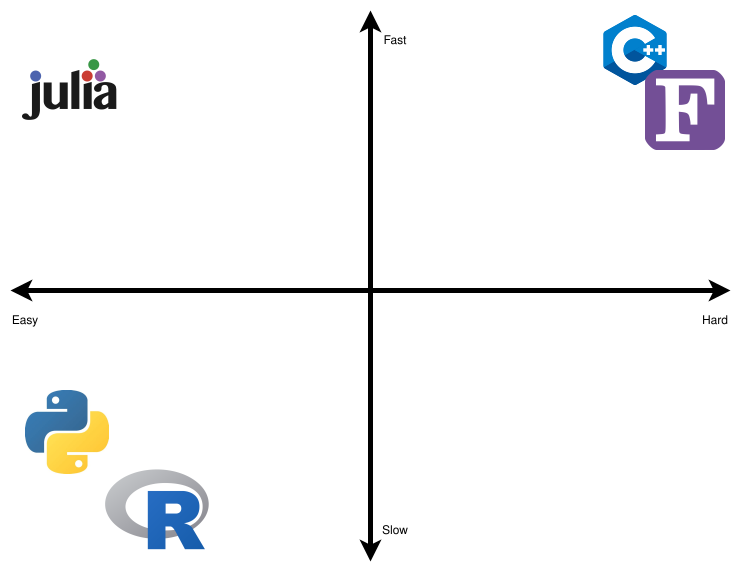
\includegraphics{images/language_comparisons.png}
\caption{Comparações entre linguagens de computação científicas: logos
para FORTRAN, C++, Python, R e Julia.}\label{fig:language_comparison}
}
\end{figure}

\textbf{Julia é rápida! Muito rápida!} Foi desenvolvida para ser veloz
desde o início. E alcança esse objetivo por meio do despacho múltiplo.
Basicamente, a ideia é gerar códigos LLVM\footnote{LLVM significa
  ``Máquina Virtual de Baixo-Nível,'' ou, em inglês, \textbf{L}ow
  \textbf{L}evel \textbf{V}irtual \textbf{M}achine. Você pode encontrar
  mais sobre a LLVM no site: (\url{http://llvm.org}).} muito eficientes.
Códigos LLVM, também conhecidos como instruções LLVM, são de
baixo-nível, ou seja, muito próximos das operações reais que seu
computador está executando. Portanto, em essência, Julia converte o
código que você escreveu --- que é fácil de se ler --- em código de
máquina LLVM, que é muito difícil para humanos lerem, mas muito fácil
para um computador. Por exemplo, se você definir uma função que recebe
um argumento e passar um inteiro para a função, Julia criará um
\passthrough{\lstinline!MethodInstance!} \emph{especializado}. Na
próxima vez que você passar um inteiro como argumento para a função,
Julia buscará o \passthrough{\lstinline!MethodInstance!} criado
anteriormente e redirecionará a execução a ele. Agora, o \textbf{grande}
truque é que você também pode fazer isso dentro de uma função que chama
uma outra função. Por exemplo, se certo tipo de dado é passado dentro da
função \passthrough{\lstinline!f!} e \passthrough{\lstinline!f!} chama a
função \passthrough{\lstinline!g!}, e se os tipos de dados passados para
\passthrough{\lstinline!g!} são conhecidos e sempre os mesmos, então a
função \passthrough{\lstinline!g!} gerada pode ser codificada de forma
pré-definida pelo Julia na função \passthrough{\lstinline!f!}! Isso
significa que Julia não precisa sequer buscar
\passthrough{\lstinline!MethodInstances!} de \passthrough{\lstinline!f!}
para \passthrough{\lstinline!g!}, pois o código consegue rodar de forma
eficiente. A compensação aqui é que existem casos onde as suposições
anteriores sobre a decodificação dos
\passthrough{\lstinline!MethodInstances!} são invalidadas. Então, o
\passthrough{\lstinline!MethodInstance!} precisa ser recriado, o que
leva tempo. Além disso, a desvantagem é que também leva tempo para
inferir o que pode ser codificado de forma pré-definida e o que não
pode. Isso explica por que Julia demora para executar um código pela
primeira vez: ela está otimizando seu código em segundo-plano. A segunda
e subsequentes execuções serão extremamente rápidas.

O compilador, por sua vez, faz o que ele faz de melhor: otimiza o código
de máquina\footnote{se quer saber mais sobre como Julia foi projetada,
  acesse \protect\hyperlink{ref-bezanson2017julia}{Bezanson et al.}
  (\protect\hyperlink{ref-bezanson2017julia}{2017}).}. Você encontra
\href{https://julialang.org/benchmarks/}{benchmarks} para Julia e para
outras linguagens aqui. Figure~\ref{fig:benchmarks} foi retirado da
\href{https://julialang.org/benchmarks/}{seção de Benchmarks do site de
Julia\footnote{observe que os resultados de Julia descritos acima não
  incluem o tempo de compilação.}}. Como você pode perceber, Julia é
\textbf{de fato} rápida.

\begin{figure}
\hypertarget{fig:benchmarks}{%
\centering
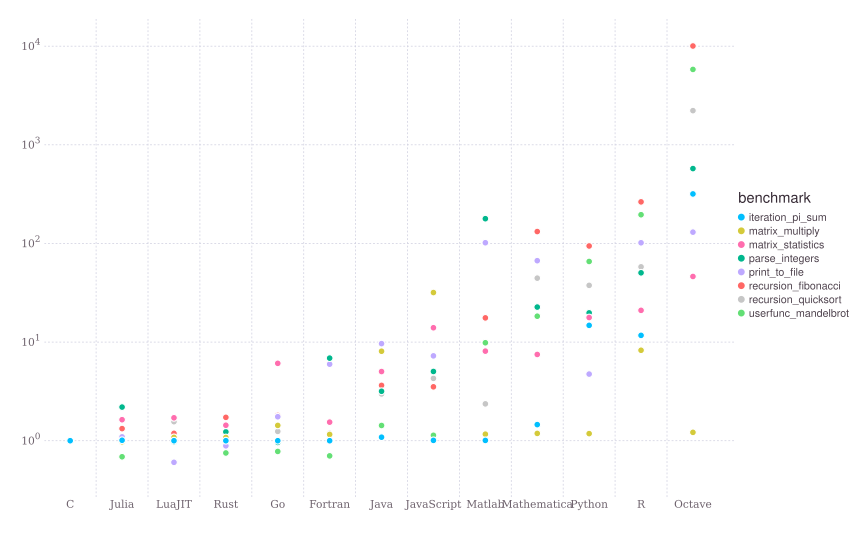
\includegraphics{images/benchmarks.png}
\caption{Julia versus outras linguagens de
programação.}\label{fig:benchmarks}
}
\end{figure}

Nós realmente acreditamos em Julia. Caso contrário, não teríamos escrito
este livro. Nós acreditamos que Julia é \textbf{o futuro da computação
científica e da análise de dados científicos}. Ela permite que o usuário
desenvolva códigos rápidos e poderosos com uma sintaxe simples.
Normalmente, pesquisadores desenvolvem códigos usando linguagens fáceis,
mas muito lentas. Uma vez que o código rode corretamente e cumpra seus
objetivos, aí começa o processo de conversão do código para uma
linguagem rápida, porém difícil. Esse é o ``problema das duas
linguagens'' e discutiremos ele melhor a seguir.

\hypertarget{sec:two_language}{%
\subsection{O Problema das Duas Linguagens}\label{sec:two_language}}

O ``Problema das Duas Linguagens'' é bastante comum na computação
científica, quando um pesquisador concebe um algoritmo, ou quando
desenvolve uma solução para um problema, ou mesmo quando realiza algum
tipo de análise. Em seguida, a solução é prototipada em uma linguagem
fácil de codificar (como Python ou R). Se o protótipo funciona, o
pesquisador codifica em uma linguagem rápida que, em geral, não é fácil
de prototipar (como C++ ou FORTRAN). Assim, temos duas linguagens
envolvidas no processo de desenvolvimento de uma nova solução. Uma que é
fácil de prototipar, mas não é adequada para implementação
(principalmente por ser lenta). E outra que não é tão simples de
codificar e, consequentemente, não é fácil de prototipar, mas adequada
para implementação porque é rápida. Julia evita esse tipo de situação
por ser a \textbf{a mesma linguagem que você prototipa (fácil de usar) e
implementa a solução (rápida)}.

Além disso, Julia permite que você use \textbf{caracteres Unicode como
variáveis ou parâmetros}. Isso significa que não é preciso mais usar
\passthrough{\lstinline!sigma!} ou \passthrough{\lstinline!sigma\_i!}:
ao invés disso use apenas \(σ\) ou \(σᵢ\) como você faria em notação
matemática. Quando você vê o código de um algoritmo ou para uma equação
matemática, você vê quase a mesma notação e expressões idiomáticas.
Chamamos esse recurso poderoso de \textbf{``Relação Um para Um entre
Código e Matemática''}.

Acreditamos que o ``Problema das Duas Linguagens'' e a ``Relação Um para
Um entre Código e Matemática'' são melhor descritos por um dos criadores
de Julia, Alan Edelman, em um \href{https://youtu.be/qGW0GT1rCvs}{TEDx
Talk} (\protect\hyperlink{ref-tedxtalksProgrammingLanguageHeal2020}{TEDx
Talks, 2020}).

\hypertarget{sec:multiple_dispatch}{%
\subsection{Despacho Múltiplo}\label{sec:multiple_dispatch}}

Despacho múltiplo é um recurso poderoso que nos permite estender funções
existentes ou definir comportamento personalizado e complexo para novos
tipos. Suponha que você queira definir dois novos
\passthrough{\lstinline!struct!}s para denotar dois animais diferentes:

\begin{lstlisting}[language=Julia]
abstract type Animal end
struct Fox <: Animal
    weight::Float64
end
struct Chicken <: Animal
    weight::Float64
end
\end{lstlisting}

Basicamente, isso diz ``defina uma raposa, que é um animal'' e ``defina
uma galinha, que é um animal.'' Em seguida, podemos ter uma raposa
chamada Fiona e uma galinha chamada Big Bird.

\begin{lstlisting}[language=Julia]
fiona = Fox(4.2)
big_bird = Chicken(2.9)
\end{lstlisting}

A seguir, queremos saber quanto elas pesam juntas, para o qual podemos
escrever uma função:

\begin{lstlisting}[language=Julia]
combined_weight(A1::Animal, A2::Animal) = A1.weight + A2.weight
\end{lstlisting}

\begin{lstlisting}[language=Output]
combined_weight (generic function with 1 method)
\end{lstlisting}

E queremos saber se elas vão se dar bem. Uma maneira de implementar isso
é usar condicionais:

\begin{lstlisting}[language=Julia]
function naive_trouble(A::Animal, B::Animal)
    if A isa Fox && B isa Chicken
        return true
    elseif A isa Chicken && B isa Fox
        return true
    elseif A isa Chicken && B isa Chicken
        return false
    end
end
\end{lstlisting}

\begin{lstlisting}[language=Output]
naive_trouble (generic function with 1 method)
\end{lstlisting}

Agora, vamos ver se deixar Fiona e Big Bird juntas daria problema:

\begin{lstlisting}[language=Julia]
naive_trouble(fiona, big_bird)
\end{lstlisting}

\begin{lstlisting}[language=Output]
true
\end{lstlisting}

OK, isso parece correto. Escrevendo a função
\passthrough{\lstinline!naive\_trouble!} parece ser o suficiente. No
entanto, usar despacho múltiplo para criar uma nova função
\passthrough{\lstinline!trouble!} pode ser benéfico. Vamos criar novas
funções:

\begin{lstlisting}[language=Julia]
trouble(F::Fox, C::Chicken) = true
trouble(C::Chicken, F::Fox) = true
trouble(C1::Chicken, C2::Chicken) = false
\end{lstlisting}

\begin{lstlisting}[language=Output]
trouble (generic function with 3 methods)
\end{lstlisting}

Depois da definição dos métodos, \passthrough{\lstinline!trouble!}
fornece o mesmo resultado que \passthrough{\lstinline!naive\_trouble!}.
Por exemplo:

\begin{lstlisting}[language=Julia]
trouble(fiona, big_bird)
\end{lstlisting}

\begin{lstlisting}[language=Output]
true
\end{lstlisting}

E deixar Big Bird sozinha com outra galinha chamada Dora também é bom

\begin{lstlisting}[language=Julia]
dora = Chicken(2.2)
trouble(dora, big_bird)
\end{lstlisting}

\begin{lstlisting}[language=Output]
false
\end{lstlisting}

Portanto, neste caso, a vantagem do despacho múltiplo é que você pode
apenas declarar tipos e Julia encontrará o método correto para seus
tipos. Ainda mais, para muitos casos quando o despacho múltiplo é usado
dentro do código, o compilador Julia irá realmente otimizar as chamadas
de função. Por exemplo, poderíamos escrever:

\begin{lstlisting}
function trouble(A::Fox, B::Chicken, C::Chicken)
    return trouble(A, B) || trouble(B, C) || trouble(C, A)
end
\end{lstlisting}

Dependendo do contexto, Julia pode otimizar isso para:

\begin{lstlisting}
function trouble(A::Fox, B::Chicken, C::Chicken)
    return true || false || true
end
\end{lstlisting}

porque o compilador \textbf{sabe} que \passthrough{\lstinline!A!} é a
raposa, \passthrough{\lstinline!B!} é a galinha e então isso pode ser
substituído pelo conteúdo do método
\passthrough{\lstinline!trouble(F::Fox, C::Chicken)!}. O mesmo vale para
\passthrough{\lstinline!trouble(C1::Chicken, C2::Chicken)!}. Em seguida,
o compilador pode otimizar isso para:

\begin{lstlisting}
function trouble(A::Fox, B::Chicken, C::Chicken)
    return true
end
\end{lstlisting}

Outro benefício do despacho múltiplo é que quando outra pessoa chega e
quer comparar os animais existentes com seu animal, uma zebra por
exemplo, é possível. Em seu pacote, eles podem definir um Zebra:

\begin{lstlisting}[language=Julia]
struct Zebra <: Animal
    weight::Float64
end
\end{lstlisting}

e também como as interações com os animais existentes seriam:

\begin{lstlisting}[language=Julia]
trouble(F::Fox, Z::Zebra) = false
trouble(Z::Zebra, F::Fox) = false
trouble(C::Chicken, Z::Zebra) = false
trouble(Z::Zebra, F::Fox) = false
\end{lstlisting}

\begin{lstlisting}[language=Output]
trouble (generic function with 6 methods)
\end{lstlisting}

Agora, podemos ver se Marty (nossa zebra) está a salvo com Big Bird:

\begin{lstlisting}[language=Julia]
marty = Zebra(412)
trouble(big_bird, marty)
\end{lstlisting}

\begin{lstlisting}[language=Output]
false
\end{lstlisting}

Ainda melhor, conseguimos calcular \textbf{o peso combinado de zebras e
outros animais sem definir qualquer função extra}:

\begin{lstlisting}[language=Julia]
combined_weight(big_bird, marty)
\end{lstlisting}

\begin{lstlisting}[language=Output]
414.9
\end{lstlisting}

Então, em resumo, o código que foi escrito pensando apenas para Raposa e
Galinha funciona para tipos que \textbf{ele nunca tinham visto}! Na
prática, isso significa que Julia facilita o reuso do código de outros
projetos.

Se você está tão animado quanto nós com o despacho múltiplo, aqui estão
mais dois exemplos aprofundados. O primeiro é uma
\href{https://storopoli.io/Bayesian-Julia/pages/1_why_Julia/\#example_one-hot_vector}{rápida
e elegante implementação de um vetor one-hot} por
\protect\hyperlink{ref-storopoli2021bayesianjulia}{Storopoli}
(\protect\hyperlink{ref-storopoli2021bayesianjulia}{2021}). O segundo é
uma entrevista com \href{https://www.chrisrackauckas.com/}{Christopher
Rackauckas} no \href{https://youtu.be/moyPIhvw4Nk?t=2107}{canal do
YouTube de Tanmay Bakshi} (assista do minuto 35:07 em diante)
(\protect\hyperlink{ref-tanmaybakshiBakingKnowledgeMachine2021}{tanmay
bakshi, 2021}). Chris explica que, enquanto utilizava o
\href{https://diffeq.sciml.ai/dev/}{\passthrough{\lstinline!DifferentialEquations.jl!}},
um pacote que ele desenvolveu e mantém atualmente, um usuário registrou
um problema que seu solucionador de Equações Diferenciais Ordinais (EDO)
com quaternions baseado em GPU não funcionava. Chris ficou bastante
surpreso com este pedido, já que ele não esperava que alguém combinasse
cálculos da GPU com quaternions e resolvendo EDOs. Ele ficou ainda mais
surpreso quando descobriu que o usuário cometeu um pequeno erro e que
tudo funcionou. A maior parte do mérito é devido ao múltiplo despacho e
alto compartilhamento de código/tipos definidos pelo usuário.

Para concluir, pensamos que o despacho múltiplo é melhor explicado por
um dos criadores de Julia: \href{https://youtu.be/kc9HwsxE1OY}{Stefan
Karpinski na JuliaCon 2019}.

\hypertarget{sec:julia_wild}{%
\section{Julia Por Aí}\label{sec:julia_wild}}

Em Section~\ref{sec:julia_accomplish}, explicamos por que achamos que
Julia é uma linguagem de programação única. Mostramos exemplos simples
sobre os principais recursos de Julia. Se você quiser se aprofundar em
como Julia está sendo usada, temos alguns \textbf{casos de uso
interessantes}:

\begin{enumerate}
\def\labelenumi{\arabic{enumi}.}
\tightlist
\item
  NASA usa Julia em um supercomputador que analisa
  \href{https://exoplanets.nasa.gov/news/1669/seven-rocky-trappist-1-planets-may-be-made-of-similar-stuff/}{``o
  maior lote de planetas do tamanho da Terra já encontrado''} e alcançou
  uma extraordinária otimização que tornou a execução \textbf{1.000x
  mais rápida} para catalogar 188 milhões de objetos astronômicos em 15
  minutos.
\item
  \href{https://clima.caltech.edu/}{A Aliança para a Modelagem Climática
  (Climate Model Alliance - CliMa)} usa Julia para \textbf{modelar o
  clima na GPU e CPU}. Lançado em 2018 em colaboração com pesquisadores
  da Caltech, do NASA Jet Propulsion Laboratory, e da Naval Postgraduate
  School, a CliMA está utilizando o progresso recente da ciência
  computacional para desenvolver um modelo do sistema terrestre que pode
  prever secas, ondas de calor e chuva com precisão e velocidade sem
  precedentes.
\item
  \href{https://youtu.be/19zm1Fn0S9M}{O Departamento de Aviação Federal
  dos Estados Unidos (US Federal Aviation Administration - FAA) está
  desenvolvendo um \textbf{Sistema de Prevenção de Colisões Aéreas
  (Airborne Collision Avoidance System - ACAS-X)} usando Julia}. Esse é
  um bom exemplo do ``Problema das Duas Linguagens'' (see
  Section~\ref{sec:julia_accomplish}). Soluções anteriores usavam Matlab
  para desenvolver os algoritmos e C++ para uma implementação mais
  rápida. Agora, FAA usa uma única linguagem para tudo isso: Julia.
\item
  \href{https://juliacomputing.com/case-studies/pfizer/}{\textbf{Aceleração
  de 175x} para modelos de farmacologia da Pfizer usando GPUs em Julia}.
  Foi apresentado como um
  \href{https://chrisrackauckas.com/assets/Posters/ACoP11_Poster_Abstracts_2020.pdf}{poster}
  na 11ª American Conference of Pharmacometrics (ACoP11) e
  \href{https://web.archive.org/web/20210121164011/https://www.go-acop.org/abstract-awards}{ganhou
  um prêmio de qualidade}.
\item
  \href{https://discourse.julialang.org/t/julia-and-the-satellite-amazonia-1/57541}{O
  Subsistema de Controle de Atitude e Órbita (Attitude and Orbit Control
  Subsystem - AOCS) do satélite brasileiro Amazonia-1 é \textbf{escrito
  100\% em Julia}} por Ronan Arraes Jardim Chagas
  (\url{https://ronanarraes.com/}).
\item
  \href{https://youtu.be/NY0HcGqHj3g}{O Banco Nacional de
  Desenvolvimento Econômico e Social (BNDES) do Brasil abandonou uma
  solução paga e optou pela modelagem em Julia (que é código aberto) e
  teve uma otimização de velocidade de execução em um fator de
  \textbf{10x}.}
\end{enumerate}

Se isso não for suficiente, existem mais estudos de caso em
\href{https://juliacomputing.com/case-studies/}{Julia Computing
website}.

\hypertarget{sec:julia_basics}{%
\chapter{Básico de Julia}\label{sec:julia_basics}}

\begin{quote}
\textbf{\emph{OBSERVAÇÃO:}} Neste capítulo, descreveremos o básico de
Julia como linguagem de programação. Por favor, note que isso não é
\emph{estritamente necessário} para você usar Julia como uma ferramenta
de manipulação e visualização de dados. Ter um conhecimento básico de
Julia definitivamente o tornará mais \emph{eficaz} e \emph{eficiente} no
uso de Julia. No entanto, se você preferir começar imediatamente, pode
pular para Section~\ref{sec:dataframes} e aprender sobre dados tabulares
em \passthrough{\lstinline!DataFrames.jl!}.
\end{quote}

Aqui, vamos trazer uma visão mais geral sobre a linguagem Julia,
\emph{não} algo aprofundado. Se você já está familiarizado e confortável
com outras linguagens de programação, nós encorajamos você a ler a
documentação de Julia (\url{https://docs.julialang.org/}). Os documentos
são um excelente recurso para você se aprofundar em Julia. Eles cobrem
todos os fundamentos e casos extremos, mas podem ser complicados,
especialmente se você não estiver familiarizado com a leitura de
documentação de software.

Cobriremos o básico de Julia. Imagine que Julia é um carro sofisticado
repleto de recursos, como um Tesla novo. Vamos apenas explicar a você
como ``dirigir o carro, estacioná-lo e como navegar no trânsito.'' Se
você quer saber o que ``todos os botões no volante e painel fazem,''
este não é o livro que você está procurando.

\hypertarget{sec:syntax}{%
\section{Sintaxe da linguagem}\label{sec:syntax}}

Julia é uma \textbf{linguagem de tipagem dinâmica} com um compilador
just-in-time. Isso significa que você não precisa compilar seu programa
antes de executá-lo, como precisaria fazer com C++ ou FORTRAN. Em vez
disso, Julia pegará seu código, adivinhará os tipos quando necessário e
compilará partes do código antes de executá-lo. Além disso, você não
precisa especificar explicitamente cada tipo. Julia vai inferir os tipos
para você na hora.

As principais diferenças entre Julia e outras linguagens dinâmicas como
R e Python são: Primeiro, Julia \textbf{permite ao usuário especificar
declarações de tipo}. Você já viu algumas declarações de tipo em
\emph{Por que Julia?} (Section~\ref{sec:why_julia}): eles são aqueles
dois pontos duplos \passthrough{\lstinline!::!} que às vezes vem depois
das variáveis. No entanto, se você não quiser especificar o tipo de suas
variáveis ou funções, Julia terá o prazer de inferir (adivinhar) para
você.

Em segundo lugar, Julia permite que os usuários definam o comportamento
da função de acordo com combinações diversas de tipos de argumento por
meio do despacho múltiplo. Também falamos sobre despacho múltiplo em
Section~\ref{sec:julia_accomplish}. Por meio do despacho múltiplo, nós
definimos um comportamento diferente de uma função para um determinado
tipo quando escrevemos uma nova função com o mesmo nome da função
anterior, mas cuja assinatura contém a especifcação deste tipo em seus
argumentos.

\hypertarget{sec:variable}{%
\subsection{Variáveis}\label{sec:variable}}

As variáveis são valores que você diz ao computador para armazenar com
um nome específico, para que você possa recuperar ou alterar seu valor
posteriormente. Julia tem diversos tipos de variáveis, mas, em ciência
de dados, usamos principalmente:

\begin{itemize}
\tightlist
\item
  Números inteiros: \passthrough{\lstinline!Int64!}
\item
  Números reais: \passthrough{\lstinline!Float64!}
\item
  Booleanas: \passthrough{\lstinline!Bool!}
\item
  Strings: \passthrough{\lstinline!String!}
\end{itemize}

Inteiros e números reais são armazenados usando 64 bits por padrão, é
por isso que eles têm o sufixo \passthrough{\lstinline!64!} no nome do
tipo. Se você precisar de mais ou menos precisão, existem os tipos
\passthrough{\lstinline!Int8!} ou \passthrough{\lstinline!Int128!}, por
exemplo, nos quais um maior número significa uma maior precisão. Na
maioria das vezes, isso não será um problema, então você pode
simplesmente seguir os padrões.

Criamos novas variáveis escrevendo o nome da variável à esquerda e seu
valor à direita, e no meio usamos o operador de atribuição
\passthrough{\lstinline!=!}. Por exemplo:

\begin{lstlisting}[language=Julia]
name = "Julia"
age = 9
\end{lstlisting}

\begin{lstlisting}[language=Output]
9
\end{lstlisting}

Observe que a saída de retorno da última instrução
(\passthrough{\lstinline!idade!}) foi impressa no console. Aqui, estamos
definindo duas novas variáveis: \passthrough{\lstinline!nome!} e
\passthrough{\lstinline!idade!}. Podemos recuperar seus valores
digitando os nomes dados na atribuição:

\begin{lstlisting}[language=Julia]
name
\end{lstlisting}

\begin{lstlisting}[language=Output]
Julia
\end{lstlisting}

Se quiser definir novos valores para uma variável existente, você pode
repetir os passos realizados durante a atribuição. Observe que Julia
agora substituirá o valor anterior pelo novo. Suponho que o aniversário
de Julia já passou e agora fez 10 anos:

\begin{lstlisting}[language=Julia]
age = 10
\end{lstlisting}

\begin{lstlisting}[language=Output]
10
\end{lstlisting}

Podemos fazer o mesmo com \passthrough{\lstinline!name!}. Suponha que
Julia tenha ganho alguns títulos devido à sua velocidade incrível.
Mudaríamos a variável \passthrough{\lstinline!name!} para o novo valor:

\begin{lstlisting}[language=Julia]
name = "Julia Rapidus"
\end{lstlisting}

\begin{lstlisting}[language=Output]
Julia Rapidus
\end{lstlisting}

Também podemos fazer operações em variáveis como adição ou divisão.
Vamos ver quantos anos Julia tem, em meses, multiplicando
\passthrough{\lstinline!age!} por 12:

\begin{lstlisting}[language=Julia]
12 * age
\end{lstlisting}

\begin{lstlisting}[language=Output]
120
\end{lstlisting}

Podemos inspecionar os tipos das variáveis usando a função
\passthrough{\lstinline!typeof!}:

\begin{lstlisting}[language=Julia]
typeof(age)
\end{lstlisting}

\begin{lstlisting}[language=Output]
Int64
\end{lstlisting}

A próxima pergunta então se torna: ``O que mais posso fazer com os
inteiros?'' Há uma função boa e útil,
\passthrough{\lstinline!methodswith!} que expõe todas as funções
disponíveis, junto com sua assinatura, para um certo tipo. Aqui, vamos
restringir a saída às primeiras 5 linhas:

\begin{lstlisting}[language=Julia]
first(methodswith(Int64), 5)
\end{lstlisting}

\begin{lstlisting}[language=Output]
[1] logmvbeta(p::Int64, a::T, b::T) where T<:Real in StatsFuns at /home/runner/.julia/packages/StatsFuns/mQJB7/src/misc.jl:22
[2] logmvbeta(p::Int64, a::Real, b::Real) in StatsFuns at /home/runner/.julia/packages/StatsFuns/mQJB7/src/misc.jl:23
[3] logmvgamma(p::Int64, a::Real) in StatsFuns at /home/runner/.julia/packages/StatsFuns/mQJB7/src/misc.jl:8
[4] read(t::HTTP.ConnectionPool.Transaction, nb::Int64) in HTTP.ConnectionPool at /home/runner/.julia/packages/HTTP/aTjcj/src/ConnectionPool.jl:232
[5] write(ctx::MbedTLS.MD, i::Union{Float16, Float32, Float64, Int128, Int16, Int32, Int64, UInt128, UInt16, UInt32, UInt64}) in MbedTLS at /home/runner/.julia/packages/MbedTLS/lqmet/src/md.jl:140
\end{lstlisting}

\hypertarget{sec:struct}{%
\subsection{Tipos definidos pelo usuário}\label{sec:struct}}

Ter apenas variáveis à disposição, sem qualquer forma de hierarquia ou
relacionamento não é o ideal. Em Julia, podemos definir essa espécie de
dado estruturado com um \passthrough{\lstinline!struct!} (também
conhecido como tipo composto). Dentro de cada
\passthrough{\lstinline!struct!}, você pode especificar um conjunto de
campos \passthrough{\lstinline!field!}s. Eles diferem dos tipos
primitivos (por exemplo, inteiro e flutuantes) que já são definidos por
padrão dentro do núcleo da linguagem Julia. Já que a maioria dos
\passthrough{\lstinline!struct!} são definidos pelo usuário, eles são
conhecidos como tipos definidos pelo usuário.

Por exemplo, vamos criar um \passthrough{\lstinline!struct!} para
representar linguagens de programação científica em código aberto.
Também definiremos um conjunto de campos junto com os tipos
correspondentes dentro do \passthrough{\lstinline!struct!}:

\begin{lstlisting}[language=Julia]
struct Language
    name::String
    title::String
    year_of_birth::Int64
    fast::Bool
end
\end{lstlisting}

Para inspecionar os nomes dos campos, você pode usar o
\passthrough{\lstinline!fieldnames!} e passar o
\passthrough{\lstinline!struct!} desejado como argumento:

\begin{lstlisting}[language=Julia]
fieldnames(Language)
\end{lstlisting}

\begin{lstlisting}[language=Output]
(:name, :title, :year_of_birth, :fast)
\end{lstlisting}

Para usar os \passthrough{\lstinline!struct!}, devemos instanciar
instâncias individuais (ou ``objetos''), cada um com seus próprios
valores específicos para os campos definidos dentro do
\passthrough{\lstinline!struct!}. Vamos instanciar duas instâncias, uma
para Julia e outra para Python:

\begin{lstlisting}[language=Julia]
julia = Language("Julia", "Rapidus", 2012, true)
python = Language("Python", "Letargicus", 1991, false)
\end{lstlisting}

\begin{lstlisting}[language=Output]
Language("Python", "Letargicus", 1991, false)
\end{lstlisting}

Algo importante de se notar com os \passthrough{\lstinline!struct!} é
que não podemos alterar seus valores uma vez que são instanciados.
Podemos resolver isso com \passthrough{\lstinline!mutable struct!}. Além
disso, observe que objetos mutáveis geralmente serão mais lentos e mais
propensos a erros. Sempre que possível, faça com que tudo seja
\emph{imutável}. Vamos criar uma
\passthrough{\lstinline!mutable struct!}.

\begin{lstlisting}[language=Julia]
mutable struct MutableLanguage
    name::String
    title::String
    year_of_birth::Int64
    fast::Bool
end

julia_mutable = MutableLanguage("Julia", "Rapidus", 2012, true)
\end{lstlisting}

\begin{lstlisting}[language=Output]
MutableLanguage("Julia", "Rapidus", 2012, true)
\end{lstlisting}

Suponha que queremos mudar o campo título do objeto
\passthrough{\lstinline!julia\_mutable!}. Agora podemos fazer isso já
que \passthrough{\lstinline!julia\_mutable!} é um
\passthrough{\lstinline!mutable struct!} instanciado:

\begin{lstlisting}[language=Julia]
julia_mutable.title = "Python Obliteratus"

julia_mutable
\end{lstlisting}

\begin{lstlisting}[language=Output]
MutableLanguage("Julia", "Python Obliteratus", 2012, true)
\end{lstlisting}

\hypertarget{operadores-booleanos-e-comparauxe7uxf5es-numuxe9ricas}{%
\subsection{Operadores booleanos e comparações
numéricas}\label{operadores-booleanos-e-comparauxe7uxf5es-numuxe9ricas}}

Agora que cobrimos os tipos, podemos passar para os operadores booleanos
e a comparação numérica.

Nós temos três operadores booleanos em Julia:

\begin{itemize}
\tightlist
\item
  \passthrough{\lstinline"!"}: \textbf{NOT}
\item
  \passthrough{\lstinline!\&\&!}: \textbf{AND}
\item
  \passthrough{\lstinline!||!}: \textbf{OR}
\end{itemize}

Aqui estão exemplos com alguns deles:

\begin{lstlisting}[language=Julia]
!true
\end{lstlisting}

\begin{lstlisting}[language=Output]
false
\end{lstlisting}

\begin{lstlisting}[language=Julia]
(false && true) || (!false)
\end{lstlisting}

\begin{lstlisting}[language=Output]
true
\end{lstlisting}

\begin{lstlisting}[language=Julia]
(6 isa Int64) && (6 isa Real)
\end{lstlisting}

\begin{lstlisting}[language=Output]
true
\end{lstlisting}

Com relação à comparação numérica, Julia tem três tipos principais de
comparações:

\begin{enumerate}
\def\labelenumi{\arabic{enumi}.}
\tightlist
\item
  \textbf{Igualdade}: ou algo é \emph{igual} ou \emph{não igual} em
  relação a outro

  \begin{itemize}
  \tightlist
  \item
    == ``igual''
  \item
    != ou ≠ ``não igual''
  \end{itemize}
\item
  \textbf{Menor que}: ou algo é \emph{menor que} ou \emph{menor ou igual
  a}

  \begin{itemize}
  \tightlist
  \item
    \textless{} ``menor que''
  \item
    \textless= ou ≤ ``menor ou igual a''
  \end{itemize}
\item
  \textbf{Maior que}: ou algo é \emph{maior que} ou \emph{maior ou igual
  a}

  \begin{itemize}
  \tightlist
  \item
    \textgreater{} ``maior que''
  \item
    \textgreater= ou ≥ ``maior ou igual a''
  \end{itemize}
\end{enumerate}

Aqui temos alguns exemplos:

\begin{lstlisting}[language=Julia]
1 == 1
\end{lstlisting}

\begin{lstlisting}[language=Output]
true
\end{lstlisting}

\begin{lstlisting}[language=Julia]
1 >= 10
\end{lstlisting}

\begin{lstlisting}[language=Output]
false
\end{lstlisting}

As comparações funcionam até mesmo entre tipos diferentes:

\begin{lstlisting}[language=Julia]
1 == 1.0
\end{lstlisting}

\begin{lstlisting}[language=Output]
true
\end{lstlisting}

Também podemos misturar e combinar operadores booleanos com comparações
numéricas:

\begin{lstlisting}[language=Julia]
(1 != 10) || (3.14 <= 2.71)
\end{lstlisting}

\begin{lstlisting}[language=Output]
true
\end{lstlisting}

\hypertarget{sec:function}{%
\subsection{Funções}\label{sec:function}}

Agora que já sabemos como definir variáveis e tipos personalizados como
\passthrough{\lstinline!struct!}, vamos voltar nossa atenção para as
\textbf{funções}. Em Julia, uma função \textbf{mapeia os valores de seus
argumentos para um ou mais valores de retorno}. A sintaxe básica é
assim:

\begin{lstlisting}
function function_name(arg1, arg2)
    result = stuff with the arg1 and arg2
    return result
end
\end{lstlisting}

A declaração de funções começa com a palavra-chave
\passthrough{\lstinline!function!} seguida do nome da função. Então,
entre parênteses \passthrough{\lstinline!()!}, nós definimos os
argumentos separados por uma vírgula \passthrough{\lstinline!,!}. Dentro
da função, especificamos o que queremos que Julia faça com os parâmetros
que fornecemos. Todas as variáveis que definimos dentro de uma função
são excluídas após o retorno da função. Isso é bom porque é como se
realizasse uma limpeza automática. Depois que todas as operações no
corpo da função forem concluídas, instruímos Julia a retornar o
resultado com o comando \passthrough{\lstinline!return!}. Por fim,
informamos a Julia que a definição da função terminou com a
palavra-chave \passthrough{\lstinline!end!}.

Existe também a maneira compacta de definição de funções por meio da
\textbf{forma de atribuição}:

\begin{lstlisting}
f_name(arg1, arg2) = stuff with the arg1 and arg2
\end{lstlisting}

É a \textbf{mesma função} que antes, mas definida de uma forma
diferente, mais compacta. Como regra geral, quando seu código pode caber
facilmente em uma linha de até 92 caracteres, a forma compacta é
adequada. Caso contrário, basta usar o formato mais longo com a
palavra-chave \passthrough{\lstinline!function!}. Vamos mergulhar em
alguns exemplos.

\hypertarget{sec:function_example}{%
\subsubsection{Criando novas funções}\label{sec:function_example}}

Vamos criar uma nova função que soma números:

\begin{lstlisting}[language=Julia]
function add_numbers(x, y)
    return x + y
end
\end{lstlisting}

\begin{lstlisting}[language=Output]
add_numbers (generic function with 1 method)
\end{lstlisting}

Agora, podemos usar nossa função \passthrough{\lstinline!add\_numbers!}:

\begin{lstlisting}[language=Julia]
add_numbers(17, 29)
\end{lstlisting}

\begin{lstlisting}[language=Output]
46
\end{lstlisting}

E ela também funciona com números reais (também chamados em programação
de números de ponto-flutuante ou, de forma mais curta, com o jargão
``floats''):

\begin{lstlisting}[language=Julia]
add_numbers(3.14, 2.72)
\end{lstlisting}

\begin{lstlisting}[language=Output]
5.86
\end{lstlisting}

Além disso, podemos definir comportamentos especializados para nossa
função, por meio da especificação de declarações de tipo. Suponha que
queremos ter uma função \passthrough{\lstinline!round\_number!} que se
comporta de maneira diferente se seu argumento for um
\passthrough{\lstinline!Float64!} ou \passthrough{\lstinline!Int64!}:

\begin{lstlisting}[language=Julia]
function round_number(x::Float64)
    return round(x)
end

function round_number(x::Int64)
    return x
end
\end{lstlisting}

\begin{lstlisting}[language=Output]
round_number (generic function with 2 methods)
\end{lstlisting}

Podemos ver que ela é uma função com múltiplos métodos:

\begin{lstlisting}[language=Julia]
methods(round_number)
\end{lstlisting}

\begin{lstlisting}[language=Output]
round_number(x::Float64) in Main at none:1
\end{lstlisting}

\begin{lstlisting}[language=Output]
round_number(x::Int64) in Main at none:5
\end{lstlisting}

Mas há um problema: o que acontece se quisermos arredondar um float de
32 bits, \passthrough{\lstinline!Float32!}? Ou um inteiro de 8 bits,
\passthrough{\lstinline!Int8!}?

Se você quiser que algo funcione em todos os tipos de float e inteiros,
você pode usar um \textbf{tipo abstrato} na assinatura de tipo, como
\passthrough{\lstinline!AbstractFloat!} ou
\passthrough{\lstinline!Integer!}:

\begin{lstlisting}[language=Julia]
function round_number(x::AbstractFloat)
    return round(x)
end
\end{lstlisting}

\begin{lstlisting}[language=Output]
round_number (generic function with 3 methods)
\end{lstlisting}

Agora, funcionará da forma esperada com qualquer tipo de float:

\begin{lstlisting}[language=Julia]
x_32 = Float32(1.1)
round_number(x_32)
\end{lstlisting}

\begin{lstlisting}[language=Output]
1.0
\end{lstlisting}

\begin{quote}
\textbf{\emph{OBSERVAÇÃO:}} Podemos inspecionar tipos com as funções
\passthrough{\lstinline!supertypes!} e
\passthrough{\lstinline!subtypes!}.
\end{quote}

Vamos voltar ao nosso \passthrough{\lstinline!struct!}
\passthrough{\lstinline!Language!} que definimos anteriormente. Será um
exemplo de despacho múltiplo. Vamos estender a função
\passthrough{\lstinline!Base.show!} que imprime a saída de tipos
instanciados e de \passthrough{\lstinline!struct!}.

Por padrão, uma \passthrough{\lstinline!struct!} tem um output básico,
que você pôde observar do caso do \passthrough{\lstinline!python!}.
Podemos definir um novo método \passthrough{\lstinline!Base.show!} para
nosso tipo \passthrough{\lstinline!Language!}, assim temos uma boa
impressão para nossas instâncias de linguagens de programação. Queremos
comunicar claramente os nomes, títulos e idades em anos das linguagens
de programação. A função \passthrough{\lstinline!Base.show!} aceita como
argumentos um tipo \passthrough{\lstinline!IO!} chamado
\passthrough{\lstinline!io!} seguido pelo tipo para o qual você deseja
definir o comportamento personalizado:

\begin{lstlisting}[language=Julia]
Base.show(io::IO, l::Language) = print(
    io, l.name, " ",
    2021 - l.year_of_birth, ", years old, ",
    "has the following titles: ", l.title
)
\end{lstlisting}

Agora, vamos ver como o output de \passthrough{\lstinline!python!} será:

\begin{lstlisting}[language=Julia]
python
\end{lstlisting}

\begin{lstlisting}[language=Output]
Python 30, years old, has the following titles: Letargicus
\end{lstlisting}

\hypertarget{sec:function_multiple}{%
\subsubsection{Múltiplos Valores de
Retorno}\label{sec:function_multiple}}

Uma função também pode retornar dois ou mais valores. Veja a nova função
\passthrough{\lstinline!add\_multiply!} abaixo:

\begin{lstlisting}[language=Julia]
function add_multiply(x, y)
    addition = x + y
    multiplication = x * y
    return addition, multiplication
end
\end{lstlisting}

\begin{lstlisting}[language=Output]
add_multiply (generic function with 1 method)
\end{lstlisting}

Nesse caso, podemos fazer duas coisas:

\begin{enumerate}
\def\labelenumi{\arabic{enumi}.}
\item
  Podemos, analogamente aos valores de retorno, definir duas variáveis
  para conter os valores de retorno da função, uma para cada valor de
  retorno:

  \begin{lstlisting}[language=Julia]
  return_1, return_2 = add_multiply(1, 2)
  return_2
  \end{lstlisting}

  \begin{lstlisting}[language=Output]
  2
  \end{lstlisting}
\item
  Ou podemos definir apenas uma variável para manter os valores de
  retorno da função e acessá-los com \passthrough{\lstinline!first!} ou
  \passthrough{\lstinline!last!}:

  \begin{lstlisting}[language=Julia]
  all_returns = add_multiply(1, 2)
  last(all_returns)
  \end{lstlisting}

  \begin{lstlisting}[language=Output]
  2
  \end{lstlisting}
\end{enumerate}

\hypertarget{sec:function_keyword_arguments}{%
\subsubsection{Argumentos de
Palavra-Chave}\label{sec:function_keyword_arguments}}

Algumas funções podem aceitar argumentos de palavra-chave ao invés de
argumentos posicionais. Esses argumentos são como argumentos comuns,
exceto pelo fato de serem definidos após os argumentos de função
regulares e separados por um ponto e vírgula
\passthrough{\lstinline!;!}. Por exemplo, vamos definir uma função
\passthrough{\lstinline!logarithm!} que por padrão usa base \(e\)
(2.718281828459045) como um argumento de palavra-chave. Perceba que aqui
estamos usando o tipo abstrato \passthrough{\lstinline!Real!} para que
possamos cobrir todos os tipos derivados de
\passthrough{\lstinline!Integer!} e
\passthrough{\lstinline!AbstractFloat!}, dado que ambos são subtipos de
\passthrough{\lstinline!Real!}:

\begin{lstlisting}[language=Julia]
AbstractFloat <: Real && Integer <: Real
\end{lstlisting}

\begin{lstlisting}[language=Output]
true
\end{lstlisting}

\begin{lstlisting}[language=Julia]
function logarithm(x::Real; base::Real=2.7182818284590)
    return log(base, x)
end
\end{lstlisting}

\begin{lstlisting}[language=Output]
logarithm (generic function with 1 method)
\end{lstlisting}

Funciona sem especificar o argumento \passthrough{\lstinline!base!} já
que fornecemos um \textbf{valor de argumento padrão} na declaração da
função:

\begin{lstlisting}[language=Julia]
logarithm(10)
\end{lstlisting}

\begin{lstlisting}[language=Output]
2.3025850929940845
\end{lstlisting}

E também com o argumento de palavra-chave \passthrough{\lstinline!base!}
diferente de seu valor padrão:

\begin{lstlisting}[language=Julia]
logarithm(10; base=2)
\end{lstlisting}

\begin{lstlisting}[language=Output]
3.3219280948873626
\end{lstlisting}

\hypertarget{sec:function_anonymous}{%
\subsubsection{Funções Anônimas}\label{sec:function_anonymous}}

Muitas vezes não nos importamos com o nome da função e queremos criar
uma rapidamente. O que precisamos é das \textbf{funções anônimas}. Elas
são muito usadas no fluxo de trabalho de ciência de dados em Julia. Por
exemplo, quando usamos \passthrough{\lstinline!DataFrames.jl!}
(Section~\ref{sec:dataframes}) ou \passthrough{\lstinline!Makie.jl!}
(Section~\ref{sec:DataVisualizationMakie}), às vezes precisamos de uma
função temporária para filtrar dados ou formatar os rótulos de um
gráfico. É aí que usamos as funções anônimas. Elas são especialmente
úteis quando não queremos criar uma função e uma instrução simples seria
o suficiente.

A sintaxe é simples. Nós usamos o operador \passthrough{\lstinline!->!}.
À esquerda do \passthrough{\lstinline!->!} definimos o nome do
parâmetro. E à direita do \passthrough{\lstinline!->!} definimos quais
operações queremos realizar no parâmetro que definimos à esquerda de
\passthrough{\lstinline!->!}. Segue um exemplo. Suponha que queremos
desfazer a transformação de log usando uma exponenciação:

\begin{lstlisting}[language=Julia]
map(x -> 2.7182818284590^x, logarithm(2))
\end{lstlisting}

\begin{lstlisting}[language=Output]
2.0
\end{lstlisting}

Aqui, estamos usando a função \passthrough{\lstinline!map!} para mapear
convenientemente a função anônima (primeiro argumento) para
\passthrough{\lstinline!logarithm(2)!} (segundo argumento). Como
resultado, obtemos o mesmo número, porque o logaritmo e a exponenciação
são inversos (pelo menos na base que escolhemos -- 2.7182818284590)

\hypertarget{sec:conditionals}{%
\subsection{Condicional If-Else-Elseif}\label{sec:conditionals}}

Na maioria das linguagens de programação, o usuário tem permissão para
controlar o fluxo de execução do computador. Dependendo da situação,
queremos que o computador faça uma coisa ou outra. Em Julia, podemos
controlar o fluxo de execução com as palavras-chave
\passthrough{\lstinline!if!}, \passthrough{\lstinline!elseif!} e
\passthrough{\lstinline!else!}. Estas são conhecidas como declarações
condicionais.

A palavra-chave \passthrough{\lstinline!if!} comanda Julia a avaliar uma
expressão e, dependendo se ela é verdadeira
(\passthrough{\lstinline!true!}) ou falsa
(\passthrough{\lstinline!false!}), a executar certas partes do código.
Podemos combinar várias condições \passthrough{\lstinline!if!} com a
palavra-chave \passthrough{\lstinline!elseif!} para um fluxo de controle
complexo. Assim, podemos definir uma parte alternativa a ser executada
se qualquer coisa dentro de \passthrough{\lstinline!if!}
ou\passthrough{\lstinline!elseif!} for avaliada como
\passthrough{\lstinline!true!}. Esse é o propósito da palavra-chave
\passthrough{\lstinline!else!}. Finalmente, como em todos os operadores
de palavra-chave que vimos anteriormente, devemos informar a Julia
quando a declaração condicional for concluída com a palavra-chave
\passthrough{\lstinline!end!}.

Aqui, temos um exemplo com todas as palavras-chave
\passthrough{\lstinline!if!}-\passthrough{\lstinline!elseif!}-\passthrough{\lstinline!else!}:

\begin{lstlisting}[language=Julia]
a = 1
b = 2

if a < b
    "a is less than b"
elseif a > b
    "a is greater than b"
else
    "a is equal to b"
end
\end{lstlisting}

\begin{lstlisting}[language=Output]
a is less than b
\end{lstlisting}

Podemos até envelopar isso em uma função chamada
\passthrough{\lstinline!compare!}:

\begin{lstlisting}[language=Julia]
function compare(a, b)
    if a < b
        "a is less than b"
    elseif a > b
        "a is greater than b"
    else
        "a is equal to b"
    end
end

compare(3.14, 3.14)
\end{lstlisting}

a is equal to b

\hypertarget{sec:for}{%
\subsection{Laço For}\label{sec:for}}

O clássico laço for em Julia segue uma sintaxe semelhante à das
declarações condicionais. Você começa com a palavra-chave, nessa caso
\passthrough{\lstinline!for!}. Em seguida, você especifica o que Julia
deve iterar sobre (ou, no jargão, ``loopar''), p.~ex., uma sequência.
Além disso, como em tudo mais, você deve terminar com a palavra-chave
\passthrough{\lstinline!end!}.

Então, para fazer Julia imprimir todos os números de 1 a 10, você pode
usar o seguinte laço for:

\begin{lstlisting}[language=Julia]
for i in 1:10
    println(i)
end
\end{lstlisting}

\hypertarget{sec:while}{%
\subsection{Laço While}\label{sec:while}}

O laço while é uma mistura das declarações condicionais anteriores com
os laços for. Aqui, o laço é executado toda vez que a condição é
avaliada como \passthrough{\lstinline!true!}. A sintaxe segue a mesma
forma da anterior. Começamos com a palavra-chave
\passthrough{\lstinline!while!}, seguido por uma declaração que é
avaliada em \passthrough{\lstinline!true!} ou
\passthrough{\lstinline!false!}. Como de costume, devemos terminar com a
palavra-chave \passthrough{\lstinline!end!}.

Segue um exemplo:

\begin{lstlisting}[language=Julia]
n = 0

while n < 3
    global n += 1
end

n
\end{lstlisting}

\begin{lstlisting}[language=Output]
3
\end{lstlisting}

Como pode ver, devemos usar a palavra-chave
\passthrough{\lstinline!global!}. Isso se deve ao \textbf{escopo de
variável}. Variáveis definidas dentro das declarações condicionais,
laços e funções existem apenas dentro delas. Isso é conhecido como o
\emph{escopo} da variável. Aqui, precisamos avisar Julia que o
\passthrough{\lstinline!n!} dentro do laço
\passthrough{\lstinline!while!} está no escopo global por meio do uso da
palavra-chave \passthrough{\lstinline!global!}.

Por fim, também usamos o operador \passthrough{\lstinline!+=!} que é uma
boa abreviatura para \passthrough{\lstinline!n = n + 1!}.

\hypertarget{sec:data_structures}{%
\section{Estruturas Nativas de Dados}\label{sec:data_structures}}

Julia possui diversas estruturas de dados nativas. Elas são abstrações
de dados que representam alguma forma de dado estruturado. Vamos cobrir
os mais usados. Eles contém dados homogêneos ou heterogêneos. Uma vez
que são coleções, podemos iterar sobre eles com os laços
\passthrough{\lstinline!for!}.

Nós cobriremos \passthrough{\lstinline!String!},
\passthrough{\lstinline!Tuple!}, \passthrough{\lstinline!NamedTuple!},
\passthrough{\lstinline!UnitRange!}, \passthrough{\lstinline!Arrays!},
\passthrough{\lstinline!Pair!}, \passthrough{\lstinline!Dict!},
\passthrough{\lstinline!Symbol!}.

Quando você se depara com uma estrutura de dados em Julia, você pode
encontrar métodos que a aceitam como um argumento por meio da função
\passthrough{\lstinline!methodswith!}. Em Julia, a distinção entre
métodos e funções é a seguinte: Cada função pode ter mútiplos métodos,
como mostramos anteriormente. A função
\passthrough{\lstinline!methodswith!} é boa de se ter por perto. Vejamos
o que podemos fazer com uma \passthrough{\lstinline!String!}, por
exemplo:

\begin{lstlisting}[language=Julia]
first(methodswith(String), 5)
\end{lstlisting}

\begin{lstlisting}[language=Output]
[1] write(fp::FilePathsBase.SystemPath, x::Union{String, Vector{UInt8}}) in FilePathsBase at /home/runner/.julia/packages/FilePathsBase/9kSEl/src/system.jl:380
[2] write(fp::FilePathsBase.SystemPath, x::Union{String, Vector{UInt8}}, mode) in FilePathsBase at /home/runner/.julia/packages/FilePathsBase/9kSEl/src/system.jl:380
[3] write(iod::HTTP.DebugRequest.IODebug, x::String) in HTTP.DebugRequest at /home/runner/.julia/packages/HTTP/aTjcj/src/IODebug.jl:38
[4] write(buffer::FilePathsBase.FileBuffer, x::String) in FilePathsBase at /home/runner/.julia/packages/FilePathsBase/9kSEl/src/buffer.jl:85
[5] write(io::IO, s::Union{SubString{String}, String}) in Base at strings/io.jl:244
\end{lstlisting}

\hypertarget{sec:broadcasting}{%
\subsection{Fazendo Broadcasting de Operadores e
Funções}\label{sec:broadcasting}}

Antes de mergulharmos nas estruturas de dados, precisamos conversar
sobre broadcasting (também conhecido como \emph{vetorização}) e o
operador ``dot'' \passthrough{\lstinline!.!}.

Podemos vetorizar operações matemáticas como \passthrough{\lstinline!*!}
(multiplicação) ou \passthrough{\lstinline!+!} (adição) usando o
operador dot. Por exemplo, vetorizar adição implica em mudar
\passthrough{\lstinline!+!} para \passthrough{\lstinline!.+!}:

\begin{lstlisting}[language=Julia]
[1, 2, 3] .+ 1
\end{lstlisting}

\begin{lstlisting}[language=Output]
[2, 3, 4]
\end{lstlisting}

Também funciona automaticamente com funções. (Tecnicamente, as operações
matemáticas, ou operadores infixos, também são funções, mas isso não é
tão importante saber.) Lembra da nossa função
\passthrough{\lstinline!logarithm!}?

\begin{lstlisting}[language=Julia]
logarithm.([1, 2, 3])
\end{lstlisting}

\begin{lstlisting}[language=Output]
[0.0, 0.6931471805599569, 1.0986122886681282]
\end{lstlisting}

\hypertarget{sec:function_bang}{%
\subsubsection{\texorpdfstring{Funções com exclamação
\texttt{!}}{Funções com exclamação !}}\label{sec:function_bang}}

É uma convenção de Julia acrescentar uma exclamação
\passthrough{\lstinline"!"} a nomes de funções que modificam um ou mais
de seus argumentos. Esta convenção avisa o usuário que a função
\textbf{não é pura}, ou seja, que tem \emph{efeitos colaterais}. Uma
função com efeitos colaterais é útil quando você deseja atualizar uma
grande estrutura de dados ou coleção de variáveis sem ter toda a
sobrecarga da criação de uma nova instância.

Por exemplo, podemos criar uma função que adiciona 1 a cada elemento de
um vetor \passthrough{\lstinline!V!}:

\begin{lstlisting}[language=Julia]
function add_one!(V)
    for i in 1:length(V)
        V[i] += 1
    end
    return nothing
end
\end{lstlisting}

\begin{lstlisting}[language=Julia]
my_data = [1, 2, 3]

add_one!(my_data)

my_data
\end{lstlisting}

\begin{lstlisting}[language=Output]
[2, 3, 4]
\end{lstlisting}

\hypertarget{sec:string}{%
\subsection{String}\label{sec:string}}

\textbf{Strings} são representadas delimitadas por aspas duplas:

\begin{lstlisting}[language=Julia]
typeof("This is a string")
\end{lstlisting}

\begin{lstlisting}[language=Output]
String
\end{lstlisting}

Também podemos escrever uma string multilinha:

\begin{lstlisting}[language=Julia]
text = "
This is a big multiline string.
As you can see.
It is still a String to Julia.
"
\end{lstlisting}

\begin{lstlisting}[language=Output]

This is a big multiline string.
As you can see.
It is still a String to Julia.

\end{lstlisting}

Mas, geralmente, é mais claro usar aspas triplas:

\begin{lstlisting}[language=Julia]
s = """
    This is a big multiline string with a nested "quotation".
    As you can see.
    It is still a String to Julia.
    """
\end{lstlisting}

\begin{lstlisting}[language=Output]
This is a big multiline string with a nested "quotation".
As you can see.
It is still a String to Julia.

\end{lstlisting}

Ao usar crases triplas, a tabulação e o marcador de nova linha no início
são ignorados por Julia. Isso melhora a legibilidade do código porque
você pode indentar o bloco em seu código-fonte sem que esses espaços
acabem em sua string.

\hypertarget{sec:string_concatenation}{%
\subsubsection{Concatenação de Strings}\label{sec:string_concatenation}}

Uma operação comum de string é a \textbf{concatenação de string}.
Suponha que você queira construir uma nova string que é a concatenação
de duas ou mais strings. Isso é realizado em Julia com o operador
\passthrough{\lstinline!*!} ou a função \passthrough{\lstinline!join!}.
Este símbolo pode soar como uma escolha estranha e realmente é. Por
enquanto, muitas bases de código em Julia estão usando este símbolo,
então ele permanecerá na linguagem. Se você estiver interessado, pode
ler uma discussão de 2015 sobre isso em
\url{https://github.com/JuliaLang/julia/issues/11030}.

\begin{lstlisting}[language=Julia]
hello = "Hello"
goodbye = "Goodbye"

hello * goodbye
\end{lstlisting}

\begin{lstlisting}[language=Output]
HelloGoodbye
\end{lstlisting}

Como você pode ver, está faltando um espaço entre
\passthrough{\lstinline!hello!} e \passthrough{\lstinline!goodbye!}.
Poderíamos concatenar uma string adicional \passthrough{\lstinline!" "!}
com \passthrough{\lstinline!*!}, mas isso seria complicado para mais de
duas strings. É onde a função \passthrough{\lstinline!join!} vem a
calhar. Nós apenas passamos como argumentos as strings dentro dos
colchetes \passthrough{\lstinline![]!} e, em seguida, o separador:

\begin{lstlisting}[language=Julia]
join([hello, goodbye], " ")
\end{lstlisting}

\begin{lstlisting}[language=Output]
Hello Goodbye
\end{lstlisting}

\hypertarget{sec:string_interpolation}{%
\subsubsection{Interpolação de String}\label{sec:string_interpolation}}

Concatenar strings pode ser complicado. Podemos ser muito mais
expressivos com \textbf{interpolação de string}. Funciona assim: você
especifica o que quer que seja incluído em sua string com o cifrão
\passthrough{\lstinline!$!}. Aqui está o exemplo anterior, mas agora
usando interpolação:

\begin{lstlisting}[language=Julia]
"$hello $goodbye"
\end{lstlisting}

\begin{lstlisting}[language=Output]
Hello Goodbye
\end{lstlisting}

Isso funciona mesmo dentro de funções. Vamos revisitar nossa função
\passthrough{\lstinline!test!} que foi definida em
Section~\ref{sec:conditionals}:

\begin{lstlisting}[language=Julia]
function test_interpolated(a, b)
    if a < b
        "$a is less than $b"
    elseif a > b
        "$a is greater than $b"
    else
        "$a is equal to $b"
    end
end

test_interpolated(3.14, 3.14)
\end{lstlisting}

\begin{lstlisting}[language=Output]
3.14 is equal to 3.14
\end{lstlisting}

\hypertarget{sec:string_manipulations}{%
\subsubsection{Manipulações de Strings}\label{sec:string_manipulations}}

Existem várias funções para manipular strings em Julia. Vamos demonstrar
as mais comuns. Além disso, observe que a maioria dessas funções aceita
uma
\href{https://docs.julialang.org/en/v1/manual/strings/\#Regular-Expressions}{Expressão
Regular (RegEx)} como argumentos. Não cobriremos RegEx neste livro, mas
te encorajamos a aprender sobre elas, especialmente se a maior parte de
seu trabalho usa dados textuais.

Primeiro, vamos definir uma string para brincarmos:

\begin{lstlisting}[language=Julia]
julia_string = "Julia is an amazing opensource programming language"
\end{lstlisting}

\begin{lstlisting}[language=Output]
Julia is an amazing opensource programming language
\end{lstlisting}

\begin{enumerate}
\def\labelenumi{\arabic{enumi}.}
\item
  \passthrough{\lstinline!occursin!},
  \passthrough{\lstinline!startswith!} e
  \passthrough{\lstinline!endswith!}: São condicionais (retornam
  \passthrough{\lstinline!true!} ou \passthrough{\lstinline!false!}) se
  o primeiro argumento é um:

  \begin{itemize}
  \item
    \textbf{substring} do segundo argumento

    \begin{lstlisting}[language=Julia]
    occursin("Julia", julia_string)
    \end{lstlisting}

    \begin{lstlisting}[language=Output]
    true
    \end{lstlisting}
  \item
    \textbf{prefixo} do segundo argumento

    \begin{lstlisting}[language=Julia]
    startswith("Julia", julia_string)
    \end{lstlisting}

    \begin{lstlisting}[language=Output]
    false
    \end{lstlisting}
  \item
    \textbf{sufixo} do segundo argumento

    \begin{lstlisting}[language=Julia]
    endswith("Julia", julia_string)
    \end{lstlisting}

    \begin{lstlisting}[language=Output]
    false
    \end{lstlisting}
  \end{itemize}
\item
  \passthrough{\lstinline!lowercase!},
  \passthrough{\lstinline!uppercase!},
  \passthrough{\lstinline!titlecase!} e
  \passthrough{\lstinline!lowercasefirst!}:

  \begin{lstlisting}[language=Julia]
  lowercase(julia_string)
  \end{lstlisting}

  \begin{lstlisting}[language=Output]
  julia is an amazing opensource programming language
  \end{lstlisting}

  \begin{lstlisting}[language=Julia]
  uppercase(julia_string)
  \end{lstlisting}

  \begin{lstlisting}[language=Output]
  JULIA IS AN AMAZING OPENSOURCE PROGRAMMING LANGUAGE
  \end{lstlisting}

  \begin{lstlisting}[language=Julia]
  titlecase(julia_string)
  \end{lstlisting}

  \begin{lstlisting}[language=Output]
  Julia Is An Amazing Opensource Programming Language
  \end{lstlisting}

  \begin{lstlisting}[language=Julia]
  lowercasefirst(julia_string)
  \end{lstlisting}

  \begin{lstlisting}[language=Output]
  julia is an amazing opensource programming language
  \end{lstlisting}
\item
  \passthrough{\lstinline!replace!}: introduz uma nova sintaxe, chamada
  de \passthrough{\lstinline!Pair!}

  \begin{lstlisting}[language=Julia]
  replace(julia_string, "amazing" => "awesome")
  \end{lstlisting}

  \begin{lstlisting}[language=Output]
  Julia is an awesome opensource programming language
  \end{lstlisting}
\item
  \passthrough{\lstinline!split!}: fatia uma string por um delimitador:

  \begin{lstlisting}[language=Julia]
  split(julia_string, " ")
  \end{lstlisting}

  \begin{lstlisting}[language=Output]
  SubString{String}["Julia", "is", "an", "amazing", "opensource", "programming", "language"]
  \end{lstlisting}
\end{enumerate}

\hypertarget{sec:string_conversions}{%
\subsubsection{Convertendo em/parseando
Strings}\label{sec:string_conversions}}

Muitas vezes, precisamos \textbf{converter} tipos de variáveis em Julia.
Para converter um número em uma string, podemos usar a função
\passthrough{\lstinline!string!}:

\begin{lstlisting}[language=Julia]
my_number = 123
typeof(string(my_number))
\end{lstlisting}

\begin{lstlisting}[language=Output]
String
\end{lstlisting}

Às vezes, queremos o oposto: converter uma string em um número (ou, como
se diz no jargão, parsear essa string). Julia tem uma função útil para
isso: \passthrough{\lstinline!parse!}.

\begin{lstlisting}[language=Julia]
typeof(parse(Int64, "123"))
\end{lstlisting}

\begin{lstlisting}[language=Output]
Int64
\end{lstlisting}

Às vezes, queremos jogar pelo seguro com essas conversões. É aí que
entra a função \passthrough{\lstinline!tryparse!}. Tem a mesma
funcionalidade que \passthrough{\lstinline!parse!} mas retorna um valor
do tipo solicitado ou \passthrough{\lstinline!nothing!}. Isso faz com
que a \passthrough{\lstinline!tryparse!} seja útil quando buscamos
evitar erros. Claro, você precisará lidar com todos aqueles valores
\passthrough{\lstinline!nothing!} depois.

\begin{lstlisting}[language=Julia]
tryparse(Int64, "A very non-numeric string")
\end{lstlisting}

\begin{lstlisting}[language=Output]
nothing
\end{lstlisting}

\hypertarget{sec:tuple}{%
\subsection{Tupla}\label{sec:tuple}}

Julia tem uma estrutura de dados chamada \textbf{tupla}. Ela é muito
\emph{especial} em Julia porque ela é frequentemente usada em relação às
funções. Uma vez que as funções são um recurso importante em Julia, todo
usuário precisa saber o básico das tuplas.

Uma tupla é um \textbf{contâiner de tamanho fixo que pode conter vários
tipos diferentes}. Uma tupla é um \textbf{objeto imutável}, o que
significa que não pode ser modificado após a instanciação. Para
construir uma tupla, use parênteses \passthrough{\lstinline!()!} para
delimitar o início e o fim, junto com vírgulas
\passthrough{\lstinline!,!} como delimitadores entre valores:

\begin{lstlisting}[language=Julia]
my_tuple = (1, 3.14, "Julia")
\end{lstlisting}

\begin{lstlisting}[language=Output]
(1, 3.14, "Julia")
\end{lstlisting}

Aqui, estamos criando uma tupla com três valores. Cada um dos valores é
um tipo diferente. Podemos acessá-los por meio de indexação. Assim:

\begin{lstlisting}[language=Julia]
my_tuple[2]
\end{lstlisting}

\begin{lstlisting}[language=Output]
3.14
\end{lstlisting}

Também podemos iterar sobre tuplas com a palavra-chave
\passthrough{\lstinline!for!}. E até mesmo aplicar funções sobre tuplas.
Mas nós nunca podemos \textbf{mudar qualquer valor de uma tupla} já que
elas são \textbf{imutáveis}.

Você se lembra funções que retornam vários valores em
Section~\ref{sec:function_multiple}? Vamos inspecionar o que nossa
função \passthrough{\lstinline!add\_multiply!} retorna:

\begin{lstlisting}[language=Julia]
return_multiple = add_multiply(1, 2)
typeof(return_multiple)
\end{lstlisting}

\begin{lstlisting}[language=Output]
Tuple{Int64, Int64}
\end{lstlisting}

Isso ocorre porque \passthrough{\lstinline!return a, b!} é o mesmo que
\passthrough{\lstinline!return (a, b)!}:

\begin{lstlisting}[language=Julia]
1, 2
\end{lstlisting}

\begin{lstlisting}[language=Output]
(1, 2)
\end{lstlisting}

Agora você pode ver porque tuplas e funções são frequentemente
relacionadas.

Mais uma coisa para pensarmos sobre as tuplas. \textbf{Quando você
deseja passar mais de uma variável para uma função anônima, adivinhe o
que você precisa usar? Tuplas!}

\begin{lstlisting}[language=Julia]
map((x, y) -> x^y, 2, 3)
\end{lstlisting}

\begin{lstlisting}[language=Output]
8
\end{lstlisting}

Ou ainda, mais do que dois argumentos:

\begin{lstlisting}[language=Julia]
map((x, y, z) -> x^y + z, 2, 3, 1)
\end{lstlisting}

\begin{lstlisting}[language=Output]
9
\end{lstlisting}

\hypertarget{sec:namedtuple}{%
\subsection{Tupla Nomeada}\label{sec:namedtuple}}

Às vezes, você deseja nomear os valores contidos nas tuplas. É aí que
entram as \textbf{tuplas nomeadas}. Sua funcionalidade é praticamente a
mesma das tuplas: são \textbf{imutáveis} e podem conter \textbf{todo
tipo de valor}.

A construção das tuplas nomeadas é ligeiramente diferente das tuplas.
Você tem os familiares parênteses \passthrough{\lstinline!()!} e a
vírgula \passthrough{\lstinline!,!} separadora de valor. Mas agora, você
\textbf{nomeia os valores}:

\begin{lstlisting}[language=Julia]
my_namedtuple = (i=1, f=3.14, s="Julia")
\end{lstlisting}

\begin{lstlisting}[language=Output]
(i = 1, f = 3.14, s = "Julia")
\end{lstlisting}

Podemos acessar os valores de uma tupla nomeada por meio da indexação
como em tuplas regulares ou, alternativamente, \textbf{acessá-los por
seus nomes} com o \passthrough{\lstinline!.!}:

\begin{lstlisting}[language=Julia]
my_namedtuple.s
\end{lstlisting}

\begin{lstlisting}[language=Output]
Julia
\end{lstlisting}

Encerrando nossa discussão sobre tuplas nomeadas, há uma sintaxe
\emph{rápida} importante que você verá muito no código de Julia.
Frequentemente, os usuários de Julia criam uma tupla nomeada usando o
parêntese familiar \passthrough{\lstinline!()!} e vírgulas
\passthrough{\lstinline!,!}, mas sem nomear os valores. Para fazer isso,
\textbf{comece a construção da tupla nomeada especificando primeiro um
ponto e vírgula \passthrough{\lstinline!;!} antes dos valores}. Isto é
especialmente útil quando os valores que iriam compor a tupla nomeada já
estão definidos em variáveis ou quando você deseja evitar linhas longas:

\begin{lstlisting}[language=Julia]
i = 1
f = 3.14
s = "Julia"

my_quick_namedtuple = (; i, f, s)
\end{lstlisting}

\begin{lstlisting}[language=Output]
(i = 1, f = 3.14, s = "Julia")
\end{lstlisting}

\hypertarget{sec:ranges}{%
\subsection{Ranges}\label{sec:ranges}}

Uma \textbf{range} em Julia representa um intervalo entre os limites de
início e parada. A sintaxe é \passthrough{\lstinline!start:stop!}:

\begin{lstlisting}[language=Julia]
1:10
\end{lstlisting}

\begin{lstlisting}[language=Output]
1:10
\end{lstlisting}

Como você pode ver, nosso range instanciado é do tipo
\passthrough{\lstinline!UnitRange\{T\}!} onde
\passthrough{\lstinline!T!} é o tipo de dados contido dentro de
\passthrough{\lstinline!UnitRange!}:

\begin{lstlisting}[language=Julia]
typeof(1:10)
\end{lstlisting}

\begin{lstlisting}[language=Output]
UnitRange{Int64}
\end{lstlisting}

E, se recolhermos todos os valores, temos:

\begin{lstlisting}[language=Julia]
[x for x in 1:10]
\end{lstlisting}

\begin{lstlisting}[language=Output]
[1, 2, 3, 4, 5, 6, 7, 8, 9, 10]
\end{lstlisting}

Também podemos construir ranges para outros tipos:

\begin{lstlisting}[language=Julia]
typeof(1.0:10.0)
\end{lstlisting}

\begin{lstlisting}[language=Output]
StepRangeLen{Float64, Base.TwicePrecision{Float64}, Base.TwicePrecision{Float64}, Int64}
\end{lstlisting}

Às vezes, queremos mudar o comportamento padrão do incremento do
intervalo. Podemos fazer isso adicionando um incremento específico por
meio da sintaxe da range \passthrough{\lstinline!start:step:stop!}. Por
exemplo, suponha que queremos um range de
\passthrough{\lstinline!Float64!} que vá de 0 a 1 com passos do tamanho
de 0.2:

\begin{lstlisting}[language=Julia]
0.0:0.2:1.0
\end{lstlisting}

\begin{lstlisting}[language=Output]
0.0:0.2:1.0
\end{lstlisting}

Se você quer ``materializar'' a range, transformando-a em uma coleção,
você pode usar a função \passthrough{\lstinline!collect!}:

\begin{lstlisting}[language=Julia]
collect(1:10)
\end{lstlisting}

\begin{lstlisting}[language=Output]
[1, 2, 3, 4, 5, 6, 7, 8, 9, 10]
\end{lstlisting}

Assim, temos uma array do tipo especificado no range entre os limites
que definimos. Já que estamos falando de arrays, vamos conversar sobre
eles.

\hypertarget{sec:array}{%
\subsection{Array}\label{sec:array}}

Na sua forma mais básica, \textbf{arrays} contém múltiplos objetos. Por
exemplo, elas podem armazenar múltiplos números em uma dimensão:

\begin{lstlisting}[language=Julia]
myarray = [1, 2, 3]
\end{lstlisting}

\begin{lstlisting}[language=Output]
[1, 2, 3]
\end{lstlisting}

Na maioria das vezes você quer ter \textbf{arrays de tipo único para
evitar problemas de performance}, mas observe que elas também podem
conter objetos de diferentes tipos:

\begin{lstlisting}[language=Julia]
myarray = ["text", 1, :symbol]
\end{lstlisting}

\begin{lstlisting}[language=Output]
Any["text", 1, :symbol]
\end{lstlisting}

Elas são o ``pão com manteiga'' da ciência de dados, porque as arrays
são o que está por trás da maior parte do fluxo de trabalho em
\textbf{manipulação de dados} e \textbf{visualização de dados}.

Portanto, \textbf{arrays são uma estrutura de dados essencial}.

\hypertarget{sec:array_types}{%
\subsubsection{Tipos de array}\label{sec:array_types}}

Vamos começar com os \textbf{tipos de arrays}. Existem vários, mas vamos
nos concentrar nos dois mais usados em ciência de dados:

\begin{itemize}
\tightlist
\item
  \passthrough{\lstinline!Vector\{T\}!}: array \textbf{unidimensional}.
  Escrita alternativa para \passthrough{\lstinline!Array\{T, 1\}!}.
\item
  \passthrough{\lstinline!Matrix\{T\}!}: array\textbf{bidimensional}.
  Escrita alternativa para \passthrough{\lstinline!Array\{T, 2\}!}.
\end{itemize}

Observe aqui que \passthrough{\lstinline!T!} é o tipo da array
subjacente. Então, por exemplo,
\passthrough{\lstinline!Vector\{Int64\}!} é um
\passthrough{\lstinline!Vector!} no qual todos os elementos são
\passthrough{\lstinline!Int64!}, e
\passthrough{\lstinline!Matrix\{AbstractFloat\}!} é uma
\passthrough{\lstinline!Matrix!} em que todos os elementos são subtipos
de \passthrough{\lstinline!AbstractFloat!}.

Na maioria das vezes, especialmente ao lidar com dados tabulares,
estamos usando arrays unidimensionais ou bidimensionais. Ambos são tipos
\passthrough{\lstinline!Array!} para Julia. Mas, podemos usar os
apelidos úteis \passthrough{\lstinline!Vector!} e
\passthrough{\lstinline!Matrix!} para uma sintaxe clara e concisa.

\hypertarget{sec:array_construction}{%
\subsubsection{Construção de Array}\label{sec:array_construction}}

Como \textbf{construímos} uma array? Nesta seção, começamos construindo
arrays de uma forma mais baixo-nível. Isso pode ser necessário para
escrever código de alto desempenho em algumas situações. No entanto,
isso não é necessário na maioria das situações, e podemos, com
segurança, usar métodos mais convenientes para criar arrays. Esses
métodos mais convenientes serão descritos posteriormente nesta seção.

O construtor de baixo nível para arrays em Julia é o \textbf{construtor
padrão}. Ele aceita o tipo de elemento como o parâmetro de tipo dentro
dos colchetes \passthrough{\lstinline!\{\}!} e dentro do construtor você
passará o tipo de elemento seguido pelas dimensões desejadas. É comum
inicializar vetores e matrizes com elementos indefinidos usando o
argumento para tipo \passthrough{\lstinline!undef!}. Um vetor de 10
elementos \passthrough{\lstinline!undef!}
\passthrough{\lstinline!Float64!} pode ser construído como:

\begin{lstlisting}[language=Julia]
my_vector = Vector{Float64}(undef, 10)
\end{lstlisting}

\begin{lstlisting}[language=Output]
[0.0, 6.9165829189171e-310, 6.9165829102698e-310, 0.0, 6.9165829189171e-310, 6.9165829102698e-310, 0.0, 6.9165829189171e-310, 6.9165829102698e-310, 0.0]
\end{lstlisting}

Para matrizes, uma vez que estamos lidando com objetos bidimensionais,
precisamos passar dois argumentos de dimensão dentro do construtor: um
para \textbf{linhas} e outro para \textbf{colunas}. Por exemplo, uma
matriz com 10 linhas e 2 colunas de elementos indefinidos
\passthrough{\lstinline!undef!} pode ser instanciada como:

\begin{lstlisting}[language=Julia]
my_matrix = Matrix{Float64}(undef, 10, 2)
\end{lstlisting}

\begin{lstlisting}[language=Output]
10×2 Matrix{Float64}:
 6.91659e-310  6.91659e-310
 6.91659e-310  6.91659e-310
 6.91659e-310  6.91659e-310
 6.91659e-310  6.91659e-310
 6.91659e-310  6.91659e-310
 6.91659e-310  6.91659e-310
 6.91659e-310  6.91659e-310
 6.91659e-310  6.91659e-310
 6.91659e-310  6.91659e-310
 6.91659e-310  6.91659e-310
\end{lstlisting}

Nós também temos algumas \textbf{apelidos sintáticos} para os elementos
mais comuns na construção de arrays:

\begin{itemize}
\item
  \passthrough{\lstinline!zeros!} para todos os elementos inicializados
  em zero. Observe que o tipo padrão é \passthrough{\lstinline!Float64!}
  que pode ser alterado se necessário:

  \begin{lstlisting}[language=Julia]
  my_vector_zeros = zeros(10)
  \end{lstlisting}

  \begin{lstlisting}[language=Output]
  [0.0, 0.0, 0.0, 0.0, 0.0, 0.0, 0.0, 0.0, 0.0, 0.0]
  \end{lstlisting}

  \begin{lstlisting}[language=Julia]
  my_matrix_zeros = zeros(Int64, 10, 2)
  \end{lstlisting}

  \begin{lstlisting}[language=Output]
  10×2 Matrix{Int64}:
   0  0
   0  0
   0  0
   0  0
   0  0
   0  0
   0  0
   0  0
   0  0
   0  0
  \end{lstlisting}
\item
  \passthrough{\lstinline!ones!} para todos os elementos inicializados
  em um:

  \begin{lstlisting}[language=Julia]
  my_vector_ones = ones(Int64, 10)
  \end{lstlisting}

  \begin{lstlisting}[language=Output]
  [1, 1, 1, 1, 1, 1, 1, 1, 1, 1]
  \end{lstlisting}

  \begin{lstlisting}[language=Julia]
  my_matrix_ones = ones(10, 2)
  \end{lstlisting}

  \begin{lstlisting}[language=Output]
  10×2 Matrix{Float64}:
   1.0  1.0
   1.0  1.0
   1.0  1.0
   1.0  1.0
   1.0  1.0
   1.0  1.0
   1.0  1.0
   1.0  1.0
   1.0  1.0
   1.0  1.0
  \end{lstlisting}
\end{itemize}

Para outros elementos, podemos primeiro instanciar uma array com
elementos \passthrough{\lstinline!undef!} e usar a função
\passthrough{\lstinline"fill!"} para preencher todos os elementos de uma
array com o elemento desejado. Segue um exemplo com
\passthrough{\lstinline!3.14!} (\(\pi\)):

\begin{lstlisting}[language=Julia]
my_matrix_π = Matrix{Float64}(undef, 2, 2)
fill!(my_matrix_π, 3.14)
\end{lstlisting}

\begin{lstlisting}[language=Output]
2×2 Matrix{Float64}:
 3.14  3.14
 3.14  3.14
\end{lstlisting}

Também podemos criar arrays com \textbf{literais de array}. Por exemplo,
segue uma matriz 2x2 de inteiros:

\begin{lstlisting}[language=Julia]
[[1 2]
 [3 4]]
\end{lstlisting}

\begin{lstlisting}[language=Output]
2×2 Matrix{Int64}:
 1  2
 3  4
\end{lstlisting}

Literais de array também aceitam uma especificação de tipo antes dos
colchetes \passthrough{\lstinline![]!}. Então, se quisermos a mesma
array 2x2 de antes mas agora como floats, podemos:

\begin{lstlisting}[language=Julia]
Float64[[1 2]
        [3 4]]
\end{lstlisting}

\begin{lstlisting}[language=Output]
2×2 Matrix{Float64}:
 1.0  2.0
 3.0  4.0
\end{lstlisting}

Também funciona para vetores:

\begin{lstlisting}[language=Julia]
Bool[0, 1, 0, 1]
\end{lstlisting}

\begin{lstlisting}[language=Output]
Bool[0, 1, 0, 1]
\end{lstlisting}

Você pode até \textbf{misturar e combinar} literais de array com os
construtores:

\begin{lstlisting}[language=Julia]
[ones(Int, 2, 2) zeros(Int, 2, 2)]
\end{lstlisting}

\begin{lstlisting}[language=Output]
2×4 Matrix{Int64}:
 1  1  0  0
 1  1  0  0
\end{lstlisting}

\begin{lstlisting}[language=Julia]
[zeros(Int, 2, 2)
 ones(Int, 2, 2)]
\end{lstlisting}

\begin{lstlisting}[language=Output]
4×2 Matrix{Int64}:
 0  0
 0  0
 1  1
 1  1
\end{lstlisting}

\begin{lstlisting}[language=Julia]
[ones(Int, 2, 2) [1; 2]
 [3 4]            5]
\end{lstlisting}

\begin{lstlisting}[language=Output]
3×3 Matrix{Int64}:
 1  1  1
 1  1  2
 3  4  5
\end{lstlisting}

Outra maneira poderosa de criar uma array é escrever uma
\textbf{compreensão de array}. Esta maneira de criar arrays é melhor na
maioria dos casos: evita loops, indexação e outras operações sujeitas a
erros. Você especifica o que deseja fazer dentro dos colchetes
\passthrough{\lstinline![]!}. Por exemplo, digamos que queremos criar um
vetor de quadrados de 1 a 10:

\begin{lstlisting}[language=Julia]
[x^2 for x in 1:10]
\end{lstlisting}

\begin{lstlisting}[language=Output]
[1, 4, 9, 16, 25, 36, 49, 64, 81, 100]
\end{lstlisting}

Eles também suportam múltiplas entradas:

\begin{lstlisting}[language=Julia]
[x*y for x in 1:10 for y in 1:2]
\end{lstlisting}

\begin{lstlisting}[language=Output]
[1, 2, 2, 4, 3, 6, 4, 8, 5, 10, 6, 12, 7, 14, 8, 16, 9, 18, 10, 20]
\end{lstlisting}

E condicionais:

\begin{lstlisting}[language=Julia]
[x^2 for x in 1:10 if isodd(x)]
\end{lstlisting}

\begin{lstlisting}[language=Output]
[1, 9, 25, 49, 81]
\end{lstlisting}

Tal como acontece com literais de array, você pode especificar o tipo
desejado antes dos colchetes \passthrough{\lstinline![]!}:

\begin{lstlisting}[language=Julia]
Float64[x^2 for x in 1:10 if isodd(x)]
\end{lstlisting}

\begin{lstlisting}[language=Output]
[1.0, 9.0, 25.0, 49.0, 81.0]
\end{lstlisting}

Finalmente, também podemos criar arrays com \textbf{funções de
concatenação}. Concatenação é um termo padrão em programação e significa
``acorrentar juntos.'' Por exemplo, podemos concatenar strings com
``aa'' e ``bb'' para conseguir ``aabb'':

\begin{lstlisting}[language=Julia]
"aa" * "bb"
\end{lstlisting}

aabb

E podemos concatenar arrays para criar novas arrays:

\begin{itemize}
\item
  \passthrough{\lstinline!cat!}: concatenar arrays de entrada ao longo
  de uma dimensão específica \passthrough{\lstinline!dims!}

  \begin{lstlisting}[language=Julia]
  cat(ones(2), zeros(2), dims=1)
  \end{lstlisting}

  \begin{lstlisting}[language=Output]
  [1.0, 1.0, 0.0, 0.0]
  \end{lstlisting}

  \begin{lstlisting}[language=Julia]
  cat(ones(2), zeros(2), dims=2)
  \end{lstlisting}

  \begin{lstlisting}[language=Output]
  2×2 Matrix{Float64}:
   1.0  0.0
   1.0  0.0
  \end{lstlisting}
\item
  \passthrough{\lstinline!vcat!}: concatenação vertical, uma abreviatura
  para \passthrough{\lstinline!cat(...; dims=1)!}

  \begin{lstlisting}[language=Julia]
  vcat(ones(2), zeros(2))
  \end{lstlisting}

  \begin{lstlisting}[language=Output]
  [1.0, 1.0, 0.0, 0.0]
  \end{lstlisting}
\item
  \passthrough{\lstinline!hcat!}: concatenação horizontal, uma
  abreviatura para \passthrough{\lstinline!cat(...; dims=2)!}

  \begin{lstlisting}[language=Julia]
  hcat(ones(2), zeros(2))
  \end{lstlisting}

  \begin{lstlisting}[language=Output]
  2×2 Matrix{Float64}:
   1.0  0.0
   1.0  0.0
  \end{lstlisting}
\end{itemize}

\hypertarget{sec:array_inspection}{%
\subsubsection{Inspeção de Arrays}\label{sec:array_inspection}}

Assim que tivermos arrays, o próximo passo lógico seria
\textbf{inspeciona-las}. Existem várias funções úteis que permitem ao
usuário ter uma visão de qualquer array.

É muito útil saber que \textbf{tipo de elementos} existem dentro de uma
array. Fazemos isso com \passthrough{\lstinline!eltype!}:

\begin{lstlisting}[language=Julia]
eltype(my_matrix_π)
\end{lstlisting}

\begin{lstlisting}[language=Output]
Float64
\end{lstlisting}

Depois de conhecer seus tipos, alguém pode se interessar nas
\textbf{dimensões da array}. Julia tem várias funções para inspecionar
as dimensões da array:

\begin{itemize}
\item
  \passthrough{\lstinline!length!}: número total de elementos

  \begin{lstlisting}[language=Julia]
  length(my_matrix_π)
  \end{lstlisting}

  \begin{lstlisting}[language=Output]
  4
  \end{lstlisting}
\item
  \passthrough{\lstinline!ndims!}: número de dimensões

  \begin{lstlisting}[language=Julia]
  ndims(my_matrix_π)
  \end{lstlisting}

  \begin{lstlisting}[language=Output]
  2
  \end{lstlisting}
\item
  \passthrough{\lstinline!size!}: esse é um pouco complicado. Por
  padrão, ele retornará uma tupla contendo as dimensões da array.

  \begin{lstlisting}[language=Julia]
  size(my_matrix_π)
  \end{lstlisting}

  \begin{lstlisting}[language=Output]
  (2, 2)
  \end{lstlisting}

  Você pode obter uma dimensão específica com um segundo argumento para
  \passthrough{\lstinline!size!}. Aqui, o segundo eixo são as colunas

  \begin{lstlisting}[language=Julia]
  size(my_matrix_π, 2)
  \end{lstlisting}

  \begin{lstlisting}[language=Output]
  2
  \end{lstlisting}
\end{itemize}

\hypertarget{sec:array_indexing}{%
\subsubsection{Indexação e Fatiamento de
Array}\label{sec:array_indexing}}

Às vezes, queremos inspecionar apenas certas partes de uma array.
Chamamos isso de \textbf{indexação} e \textbf{fatiamento}. Se você
quiser uma observação particular de um vetor, ou uma linha ou coluna de
uma matriz, você provavelmente precisará \textbf{indexar uma array}.

Primeiro, vou criar um vetor e uma matriz de exemplo para brincar:

\begin{lstlisting}[language=Julia]
my_example_vector = [1, 2, 3, 4, 5]

my_example_matrix = [[1 2 3]
                     [4 5 6]
                     [7 8 9]]
\end{lstlisting}

Vamos começar com vetores. Supondo que você queira o segundo elemento de
um vetor. Você usa colchetes \passthrough{\lstinline![]!} com o
\textbf{índice} desejado dentro:

\begin{lstlisting}[language=Julia]
my_example_vector[2]
\end{lstlisting}

\begin{lstlisting}[language=Output]
2
\end{lstlisting}

A mesma sintaxe segue com as matrizes. Mas, como as matrizes são arrays
bidimensionais, temos que especificar \emph{ambas} linhas e colunas.
Vamos recuperar o elemento da segunda linha (primeira dimensão) e
primeira coluna (segunda dimensão):

\begin{lstlisting}[language=Julia]
my_example_matrix[2, 1]
\end{lstlisting}

\begin{lstlisting}[language=Output]
4
\end{lstlisting}

Júlia também possui palavras-chave convencionais para o
\textbf{primeiro} e \textbf{último} elementos de uma array:
\passthrough{\lstinline!begin!} e \passthrough{\lstinline!end!}. Por
exemplo, o penúltimo elemento de um vetor pode ser recuperado como:

\begin{lstlisting}[language=Julia]
my_example_vector[end-1]
\end{lstlisting}

\begin{lstlisting}[language=Output]
4
\end{lstlisting}

Isso também funciona para matrizes. Vamos recuperar o elemento da última
linha e segunda coluna:

\begin{lstlisting}[language=Julia]
my_example_matrix[end, begin+1]
\end{lstlisting}

\begin{lstlisting}[language=Output]
8
\end{lstlisting}

Muitas vezes, não estamos só interessados em apenas um elemento da
array, mas em todo um \textbf{subconjunto de elementos da array}.
Podemos fazer isso \textbf{fatiando} uma array. Usamos a mesma sintaxe
de índice, mas adicionando dois pontos \passthrough{\lstinline!:!} para
denotar os limites a partir dos quais estamos fatiando a array. Por
exemplo, suponha que queremos obter do 2º ao 4º elemento de um vetor:

\begin{lstlisting}[language=Julia]
my_example_vector[2:4]
\end{lstlisting}

\begin{lstlisting}[language=Output]
[2, 3, 4]
\end{lstlisting}

Poderíamos fazer o mesmo com matrizes. Particularmente com matrizes, se
quisermos selecionar \textbf{todos os elementos} em uma dimensão
seguinte, podemos fazer isso com apenas dois pontos
\passthrough{\lstinline!:!}. Por exemplo, para obter todos os elementos
da segunda linha:

\begin{lstlisting}[language=Julia]
my_example_matrix[2, :]
\end{lstlisting}

\begin{lstlisting}[language=Output]
[4, 5, 6]
\end{lstlisting}

Você pode interpretar isso com algo como ``pegue a 2ª linha e todas as
colunas.''

Também suporta \passthrough{\lstinline!begin!} e
\passthrough{\lstinline!end!}:

\begin{lstlisting}[language=Julia]
my_example_matrix[begin+1:end, end]
\end{lstlisting}

\begin{lstlisting}[language=Output]
[6, 9]
\end{lstlisting}

\hypertarget{sec:array_manipulation}{%
\subsubsection{Manipulações de Array}\label{sec:array_manipulation}}

Existem várias formas para \textbf{manipular} uma array. O primeiro
seria manipular um \textbf{único elemento da array}. Nós apenas
indexamos a array pelo elemento desejado e procedemos com uma atribuição
\passthrough{\lstinline!=!}:

\begin{lstlisting}[language=Julia]
my_example_matrix[2, 2] = 42
my_example_matrix
\end{lstlisting}

\begin{lstlisting}[language=Output]
3×3 Matrix{Int64}:
 1   2  3
 4  42  6
 7   8  9
\end{lstlisting}

Ou, você pode manipular um determinado \textbf{subconjunto de elementos
da array}. Nesse caso, precisamos fatiar a array e, em seguida, atribuir
com \passthrough{\lstinline!=!}:

\begin{lstlisting}[language=Julia]
my_example_matrix[3, :] = [17, 16, 15]
my_example_matrix
\end{lstlisting}

\begin{lstlisting}[language=Output]
3×3 Matrix{Int64}:
  1   2   3
  4  42   6
 17  16  15
\end{lstlisting}

Observe que tivemos que atribuir um vetor porque nossa array fatiada é
do tipo \passthrough{\lstinline!Vector!}:

\begin{lstlisting}[language=Julia]
typeof(my_example_matrix[3, :])
\end{lstlisting}

\begin{lstlisting}[language=Output]
Vector{Int64} (alias for Array{Int64, 1})
\end{lstlisting}

A segunda maneira de manipular uma array é \textbf{alterando suas
dimensões}. Suponha que você tenha um vetor de 6 elementos e deseja
torná-lo uma matriz 3x2. Você pode fazer isso com
\passthrough{\lstinline!reshape!}, usando a array como o primeiro
argumento e uma tupla de dimensões como segundo argumento:

\begin{lstlisting}[language=Julia]
six_vector = [1, 2, 3, 4, 5, 6]
tree_two_matrix = reshape(six_vector, (3, 2))
tree_two_matrix
\end{lstlisting}

\begin{lstlisting}[language=Output]
3×2 Matrix{Int64}:
 1  4
 2  5
 3  6
\end{lstlisting}

Você pode convertê-la de volta em um vetor especificando uma tupla com
apenas uma dimensão como o segundo argumento:

\begin{lstlisting}[language=Julia]
reshape(tree_two_matrix, (6, ))
\end{lstlisting}

\begin{lstlisting}[language=Output]
[1, 2, 3, 4, 5, 6]
\end{lstlisting}

A terceira forma pela qual podemos manipular uma array é
\textbf{aplicando uma função sobre cada elemento da array}. Aqui é onde
o operador ``dot'' \passthrough{\lstinline!.!}, também conhecido como
\emph{broadcasting}, entra.

\begin{lstlisting}[language=Julia]
logarithm.(my_example_matrix)
\end{lstlisting}

\begin{lstlisting}[language=Output]
3×3 Matrix{Float64}:
 0.0      0.693147  1.09861
 1.38629  3.73767   1.79176
 2.83321  2.77259   2.70805
\end{lstlisting}

O operador dot em Julia é extremamente versátil. Você pode até mesmo
usá-lo para vetorizar operadores infixos:

\begin{lstlisting}[language=Julia]
my_example_matrix .+ 100
\end{lstlisting}

\begin{lstlisting}[language=Output]
3×3 Matrix{Int64}:
 101  102  103
 104  142  106
 117  116  115
\end{lstlisting}

Uma alternativa para fazer o broadcasting de função sobre um vetor é
usar \passthrough{\lstinline!map!}:

\begin{lstlisting}[language=Julia]
map(logarithm, my_example_matrix)
\end{lstlisting}

\begin{lstlisting}[language=Output]
3×3 Matrix{Float64}:
 0.0      0.693147  1.09861
 1.38629  3.73767   1.79176
 2.83321  2.77259   2.70805
\end{lstlisting}

Para funções anônimas, \passthrough{\lstinline!map!} geralmente é mais
legível. Por exemplo,

\begin{lstlisting}[language=Julia]
map(x -> 3x, my_example_matrix)
\end{lstlisting}

\begin{lstlisting}[language=Output]
3×3 Matrix{Int64}:
  3    6   9
 12  126  18
 51   48  45
\end{lstlisting}

é bastante claro. No entanto, a mesma operação utilizando o operador de
broadcast fica da seguinte forma:

\begin{lstlisting}[language=Julia]
(x -> 3x).(my_example_matrix)
\end{lstlisting}

\begin{lstlisting}[language=Output]
3×3 Matrix{Int64}:
  3    6   9
 12  126  18
 51   48  45
\end{lstlisting}

Além disso, \passthrough{\lstinline!map!} funciona com fatiamento:

\begin{lstlisting}[language=Julia]
map(x -> x + 100, my_example_matrix[:, 3])
\end{lstlisting}

\begin{lstlisting}[language=Output]
[103, 106, 115]
\end{lstlisting}

Finalmente, às vezes, e especialmente ao lidar com dados tabulares,
queremos aplicar uma \textbf{função sobre todos os elementos em uma
dimensão específica de uma array}. Isso pode ser feito com a função
\passthrough{\lstinline!mapslices!}. Parecido com
\passthrough{\lstinline!map!}, o primeiro argumento é a função e o
segundo argumento é a array. A única mudança é que precisamos
especificar o argumento \passthrough{\lstinline!dims!} para sinalizar em
qual dimensão queremos transformar os elementos.

Por exemplo, vamos usar \passthrough{\lstinline!mapslice!} com a função
\passthrough{\lstinline!sum!} em ambas as linhas
(\passthrough{\lstinline!dims=1!}) e colunas
(\passthrough{\lstinline!dims=2!}):

\begin{lstlisting}[language=Julia]
# rows
mapslices(sum, my_example_matrix; dims=1)
\end{lstlisting}

\begin{lstlisting}[language=Output]
1×3 Matrix{Int64}:
 22  60  24
\end{lstlisting}

\begin{lstlisting}[language=Julia]
# columns
mapslices(sum, my_example_matrix; dims=2)
\end{lstlisting}

\begin{lstlisting}[language=Output]
3×1 Matrix{Int64}:
  6
 52
 48
\end{lstlisting}

\hypertarget{sec:array_iteration}{%
\subsubsection{Iteração de array}\label{sec:array_iteration}}

Uma operação comum é \textbf{iterar sobre uma array com um laço
\passthrough{\lstinline!for!}}. O \textbf{laço
\passthrough{\lstinline!for!} regular, quando aplicado sobre uma array
retorna cada elemento}.

O exemplo mais simples é com um vetor.

\begin{lstlisting}[language=Julia]
simple_vector = [1, 2, 3]

empty_vector = Int64[]

for i in simple_vector
    push!(empty_vector, i + 1)
end

empty_vector
\end{lstlisting}

\begin{lstlisting}[language=Output]
[2, 3, 4]
\end{lstlisting}

Às vezes, você não quer iterar sobre cada elemento, mas sim sobre cada
índice da array. \textbf{Podemos usar a função
\passthrough{\lstinline!eachindex!} combinada com um loop
\passthrough{\lstinline!for!} para iterar sobre cada índice de array}.

Novamente, vamos mostrar um exemplo com um vetor:

\begin{lstlisting}[language=Julia]
forty_twos = [42, 42, 42]

empty_vector = Int64[]

for i in eachindex(forty_twos)
    push!(empty_vector, i)
end

empty_vector
\end{lstlisting}

\begin{lstlisting}[language=Output]
[1, 2, 3]
\end{lstlisting}

Nesse exemplo, o \passthrough{\lstinline!eachindex(forty\_twos)!}
retorna os índices de \passthrough{\lstinline!forty\_twos!},
nomeadamente \passthrough{\lstinline![1, 2, 3]!}.

Da mesma forma, podemos iterar sobre matrizes. O laço
\passthrough{\lstinline!for!} padrão itera primeiro sobre as colunas e
depois sobre as linhas. Ele irá primeiro percorrer todos os elementos na
coluna 1, da primeira à última linha, em seguida, ele se moverá para a
coluna 2 de maneira semelhante até cobrir todas as colunas.

Para aqueles familiarizados com outras linguagens de programação: Julia,
como a maioria das linguagens de programação científica, é ``colunar.''
Colunar significa que os elementos da coluna são armazenados lado a lado
na memória\footnote{ou, que os ponteiros de endereço de memória para os
  elementos na coluna são armazenados um ao lado do outro.}. Isso também
significa que iterar sobre os elementos em uma coluna é muito mais
rápido do que sobre os elementos em uma linha.

Ok, vamos mostrar isso em um exemplo:

\begin{lstlisting}[language=Julia]
column_major = [[1 3]
                [2 4]]

row_major = [[1 2]
             [3 4]]
\end{lstlisting}

Se fizermos um loop sobre o vetor armazenado de forma ordenada para as
colunas, então o resultado também é ordenado:

\begin{lstlisting}[language=Julia]
indexes = Int64[]

for i in column_major
    push!(indexes, i)
end

indexes
\end{lstlisting}

\begin{lstlisting}[language=Output]
[1, 2, 3, 4]
\end{lstlisting}

No entanto, o resultado não fica ordenado ao interarmos sobre a outra
matriz:

\begin{lstlisting}[language=Julia]
indexes = Int64[]

for i in row_major
    push!(indexes, i)
end

indexes
\end{lstlisting}

\begin{lstlisting}[language=Output]
[1, 3, 2, 4]
\end{lstlisting}

Muitas vezes é melhor usar funções especializadas para esses loops:

\begin{itemize}
\item
  \passthrough{\lstinline!eachcol!}: itera sobre uma array coluna a
  coluna

  \begin{lstlisting}[language=Julia]
  first(eachcol(column_major))
  \end{lstlisting}

  \begin{lstlisting}[language=Output]
  [1, 2]
  \end{lstlisting}
\item
  \passthrough{\lstinline!eachrow!}: itera sobre uma array linha a linha

  \begin{lstlisting}[language=Julia]
  first(eachrow(column_major))
  \end{lstlisting}

  \begin{lstlisting}[language=Output]
  [1, 3]
  \end{lstlisting}
\end{itemize}

\hypertarget{sec:pair}{%
\subsection{Par}\label{sec:pair}}

Em comparação com a enorme seção sobre arrays, esta seção sobre pares
será breve. \textbf{\passthrough{\lstinline!Par!} é uma estrutura de
dados que contém dois objetos} (que em geral estão relacionados um ao
outro). Construímos um par em Julia usando a seguinte sintaxe:

\begin{lstlisting}[language=Julia]
my_pair = "Julia" => 42
\end{lstlisting}

\begin{lstlisting}[language=Output]
"Julia" => 42
\end{lstlisting}

Os elementos são armazenados nos campos \passthrough{\lstinline!first!}
e \passthrough{\lstinline!second!}.

\begin{lstlisting}[language=Julia]
my_pair.first
\end{lstlisting}

\begin{lstlisting}[language=Output]
Julia
\end{lstlisting}

\begin{lstlisting}[language=Julia]
my_pair.second
\end{lstlisting}

\begin{lstlisting}[language=Output]
42
\end{lstlisting}

Mas, na maioria dos casos, é mais fácil usar
\passthrough{\lstinline!first!} e
\passthrough{\lstinline!last!}\footnote{é mais fácil porque
  \passthrough{\lstinline!first!} e \passthrough{\lstinline!last!}
  também funcionam em muitas outras coleções, então você não precisa se
  lembrar de tanta coisa.}:

\begin{lstlisting}[language=Julia]
first(my_pair)
\end{lstlisting}

\begin{lstlisting}[language=Output]
Julia
\end{lstlisting}

\begin{lstlisting}[language=Julia]
last(my_pair)
\end{lstlisting}

\begin{lstlisting}[language=Output]
42
\end{lstlisting}

Os pares serão muito usados na manipulação e visualização de dados, uma
vez que ambos \passthrough{\lstinline!DataFrames.jl!}
(Section~\ref{sec:dataframes}) e \passthrough{\lstinline!Makie.jl!}
(Section~\ref{sec:DataVisualizationMakie}) aceitam objetos do tipo
\passthrough{\lstinline!Pair!} em suas funções principais. Por exemplo,
com \passthrough{\lstinline!DataFrames.jl!} veremos que
\passthrough{\lstinline!:a => :b!} pode ser usado para renomear a coluna
\passthrough{\lstinline!:a!} para \passthrough{\lstinline!:b!}.

\hypertarget{sec:dict}{%
\subsection{Dict}\label{sec:dict}}

Se você entendeu o que é um \passthrough{\lstinline!Pair!}, então
\passthrough{\lstinline!Dict!} não será um problema. Para todos os
propósitos práticos, \textbf{\passthrough{\lstinline!Dict!}s são
mapeamentos de chaves para valores}. Por mapeamento, queremos dizer que
se você der alguma chave a um \passthrough{\lstinline!Dict!}, então o
\passthrough{\lstinline!Dict!} poderá lhe dizer qual valor pertence
àquela chave. Chaves (\passthrough{\lstinline!key!}s) e valores
(\passthrough{\lstinline!value!}s) podem ser de qualquer tipo, mas
normalmente \passthrough{\lstinline!key!}s são strings.

Existem duas maneiras de construir \passthrough{\lstinline!Dict!}s em
Julia. A primeira é passando um vetor de tuplas como
\passthrough{\lstinline!(key, value)!} para o construtor
\passthrough{\lstinline!Dict!}:

\begin{lstlisting}[language=Julia]
name2number_map = Dict([("one", 1), ("two", 2)])
\end{lstlisting}

\begin{lstlisting}[language=Output]
Dict{String, Int64} with 2 entries:
  "two" => 2
  "one" => 1
\end{lstlisting}

Existe uma sintaxe mais legível com base no tipo
\passthrough{\lstinline!Pair!} descrito acima. Você também pode passar
\passthrough{\lstinline!Pair!}s de
\passthrough{\lstinline!key => value!}s para o construtor
\passthrough{\lstinline!Dict!}:

\begin{lstlisting}[language=Julia]
name2number_map = Dict("one" => 1, "two" => 2)
\end{lstlisting}

\begin{lstlisting}[language=Output]
Dict{String, Int64} with 2 entries:
  "two" => 2
  "one" => 1
\end{lstlisting}

Você pode recuperar um \passthrough{\lstinline!value!} de um
\passthrough{\lstinline!Dict!}s ao indexá-lo pela
\passthrough{\lstinline!key!} correspondente:

\begin{lstlisting}[language=Julia]
name2number_map["one"]
\end{lstlisting}

\begin{lstlisting}[language=Output]
1
\end{lstlisting}

Para adicionar uma nova entrada, você indexa o
\passthrough{\lstinline!Dict!} pela \passthrough{\lstinline!key!}
desejada e atribui um \passthrough{\lstinline!value!} com o operador de
atribuição \passthrough{\lstinline!=!}:

\begin{lstlisting}[language=Julia]
name2number_map["three"] = 3
\end{lstlisting}

\begin{lstlisting}[language=Output]
3
\end{lstlisting}

Se você quer checar se um \passthrough{\lstinline!Dict!} tem uma certa
\passthrough{\lstinline!key!} você pode usar
\passthrough{\lstinline!keys!} e \passthrough{\lstinline!in!}:

\begin{lstlisting}[language=Julia]
"two" in keys(name2number_map)
\end{lstlisting}

\begin{lstlisting}[language=Output]
true
\end{lstlisting}

Para deletar uma \passthrough{\lstinline!key!} você pode usar a função
\passthrough{\lstinline"delete!"}:

\begin{lstlisting}[language=Julia]
delete!(name2number_map, "three")
\end{lstlisting}

\begin{lstlisting}[language=Output]
Dict{String, Int64} with 2 entries:
  "two" => 2
  "one" => 1
\end{lstlisting}

Ou, para excluir uma chave enquanto retorna seu valor, você pode usar
\passthrough{\lstinline"pop!"}:

\begin{lstlisting}[language=Julia]
popped_value = pop!(name2number_map, "two")
\end{lstlisting}

\begin{lstlisting}[language=Output]
2
\end{lstlisting}

Agora, nosso \passthrough{\lstinline!name2number\_map!} tem apenas uma
\passthrough{\lstinline!key!}:

\begin{lstlisting}[language=Julia]
name2number_map
\end{lstlisting}

\begin{lstlisting}[language=Output]
Dict{String, Int64} with 1 entry:
  "one" => 1
\end{lstlisting}

\passthrough{\lstinline!Dict!}s também são usados para manipulação de
dados por \passthrough{\lstinline!DataFrames.jl!}
(Section~\ref{sec:dataframes}) e para visualização de dados por
\passthrough{\lstinline!Makie.jl!}
(Section~\ref{sec:DataVisualizationMakie}). Logo, é importante conhecer
suas funcionalidades básicas.

Existe outra maneira útil de construir \passthrough{\lstinline!Dict!}s.
Suponha que você tenha dois vetores e deseja construir um
\passthrough{\lstinline!Dict!} com um deles como se fosse
\passthrough{\lstinline!key!}s e outro como se fosse
\passthrough{\lstinline!value!}s. Você pode fazer isso com uma função
\passthrough{\lstinline!zip!} que ``junta'' dois objetos (como um
zíper):

\begin{lstlisting}[language=Julia]
A = ["one", "two", "three"]
B = [1, 2, 3]

name2number_map = Dict(zip(A, B))
\end{lstlisting}

\begin{lstlisting}[language=Output]
Dict{String, Int64} with 3 entries:
  "two" => 2
  "one" => 1
  "three" => 3
\end{lstlisting}

Por exemplo, agora podemos obter o número 3 via:

\begin{lstlisting}[language=Julia]
name2number_map["three"]
\end{lstlisting}

\begin{lstlisting}[language=Output]
3
\end{lstlisting}

\hypertarget{sec:symbol}{%
\subsection{Símbolo}\label{sec:symbol}}

\passthrough{\lstinline!Symbol!} na verdade \emph{não} é uma estrutura
de dados. É um tipo e se comporta de modo muito parecido com uma string.
Em vez de colocar o texto entre aspas, um símbolo começa com dois pontos
(:) e pode conter sublinhados:

\begin{lstlisting}[language=Julia]
sym = :some_text
\end{lstlisting}

\begin{lstlisting}[language=Output]
:some_text
\end{lstlisting}

Podemos facilmente converter um símbolo em string e vice-versa:

\begin{lstlisting}[language=Julia]
s = string(sym)
\end{lstlisting}

\begin{lstlisting}[language=Output]
some_text
\end{lstlisting}

\begin{lstlisting}[language=Julia]
sym = Symbol(s)
\end{lstlisting}

\begin{lstlisting}[language=Output]
:some_text
\end{lstlisting}

Um benefício simples dos símbolos é que você digita um caractere a
menos, ou seja, \passthrough{\lstinline!:some\_text!} versus
\passthrough{\lstinline!"some text"!}. Usamos muito
\passthrough{\lstinline!Symbol!}s na manipulação de dados com o package
\passthrough{\lstinline!DataFrames.jl!} (Section~\ref{sec:dataframes}) e
em visualização de dados com o package
\passthrough{\lstinline!Makie.jl!}
(Section~\ref{sec:DataVisualizationMakie}).

\hypertarget{sec:splat}{%
\subsection{Operador Splat}\label{sec:splat}}

Em Julia, temos o operador ``splat'' \passthrough{\lstinline!...!} que é
usado em chamadas de função como uma \textbf{sequência de argumentos}.
Ocasionalmente, usaremos o splat em algumas chamadas de função nos
capítulos sobre \textbf{manipulação de dados} e \textbf{visualização de
dados}.

A maneira mais intuitiva de aprender sobre o splat é com um exemplo. A
função \passthrough{\lstinline!add\_elements!} abaixo leva três
argumentos para serem somados:

\begin{lstlisting}[language=Julia]
add_elements(a, b, c) = a + b + c
\end{lstlisting}

\begin{lstlisting}[language=Output]
add_elements (generic function with 1 method)
\end{lstlisting}

Agora, suponha que temos uma coleção com três elementos. A maneira
ingênua de fazer isso seria fornecer à função todos os três elementos
como argumentos de função:

\begin{lstlisting}[language=Julia]
my_collection = [1, 2, 3]

add_elements(my_collection[1], my_collection[2], my_collection[3])
\end{lstlisting}

\begin{lstlisting}[language=Output]
6
\end{lstlisting}

Aqui é que usamos o operador ``splat'' \passthrough{\lstinline!...!} que
pega uma coleção (geralmente uma array, vetor, tupla ou range) e a
converte em uma sequência de argumentos:

\begin{lstlisting}[language=Julia]
add_elements(my_collection...)
\end{lstlisting}

\begin{lstlisting}[language=Output]
6
\end{lstlisting}

O \passthrough{\lstinline!...!} deve ser incluído após a coleção que
queremos espalhar ou ``splat'' em uma sequência de argumentos. Ambos os
exemplos apresentados acima têm o mesmo resultado:

\begin{lstlisting}[language=Julia]
add_elements(my_collection...) == add_elements(my_collection[1], my_collection[2], my_collection[3])
\end{lstlisting}

\begin{lstlisting}[language=Output]
true
\end{lstlisting}

Sempre que Julia vê um operador splat dentro de uma chamada de função,
ele será convertido em uma sequência de argumentos para todos os
elementos da coleção separados por vírgulas.

Também funciona para ranges:

\begin{lstlisting}[language=Julia]
add_elements(1:3...)
\end{lstlisting}

\begin{lstlisting}[language=Output]
6
\end{lstlisting}

\hypertarget{sec:filesystem}{%
\section{Sistema de Arquivos}\label{sec:filesystem}}

Em ciência de dados, a maioria dos projetos é realizada em um esforço
colaborativo. Compartilhamos código, dados, tabelas, figuras e assim por
diante. Por trás de tudo, está o \textbf{sistema de arquivos do sistema
operacional (SO)}. Em um mundo perfeito, o mesmo programa daria a
\textbf{mesma} saída quando executado em sistemas operacionais
\textbf{diferentes}. Infelizmente, nem sempre é esse o caso. Um exemplo
disso é a diferença entre os caminhos do Windows, tal como
\passthrough{\lstinline!C:\\\\user\\john\\!}, e do Linux, como
\passthrough{\lstinline!/home/john!}. Por isso é importante discutir as
\textbf{melhores práticas em sistema de arquivos}.

Julia tem recursos de sistema de arquivos nativos que \textbf{lidam com
as diferenças entre os sistemas operacionais}. Eles estão localizados no
módulo
\href{https://docs.julialang.org/en/v1/base/file/}{\passthrough{\lstinline!Filesystem!}}
da biblioteca central \passthrough{\lstinline!Base!} de Julia.

Sempre que você estiver lidando com arquivos como CSV, Excel ou qualquer
outro script de Julia, certifique-se de que seu código \textbf{funciona
em sistemas de arquivos de SOs diferentes}. Isso é facilmente realizado
com as funções \passthrough{\lstinline!joinpath!},
\passthrough{\lstinline!@\_\_FILE\_\_!} e
\passthrough{\lstinline!pkgdir!}.

Se você escrever seu código em um pacote, você pode usar
\passthrough{\lstinline!pkgdir!} para obter o diretório raiz do pacote.
Por exemplo, para o pacote de Julia Data Science (JDS) que usamos para
produzir este livro:

/home/runner/work/JuliaDataScience-PT/JuliaDataScience-PT

como você pode ver, o código para produzir este livro foi executado em
um computador Linux. Se você está usando um script, você pode obter a
localização do arquivo de script via

\begin{lstlisting}
root = dirname(@__FILE__)
\end{lstlisting}

O bom desses dois comandos é que eles são independentes de como o
usuário iniciou o Julia. Em outras palavras, não importa se o usuário
iniciou o programa com \passthrough{\lstinline!julia scripts/script.jl!}
ou \passthrough{\lstinline!julia script.jl!}, em ambos os casos os
caminhos são os mesmos.

A próxima etapa seria incluir o caminho relativo a partir de
\passthrough{\lstinline!root!} para o nosso arquivo desejado. Uma vez
que diferentes sistemas operacionais têm maneiras diferentes de
construir caminhos relativos com subpastas (alguns usam barras
\passthrough{\lstinline!/!} enquanto outros podem usar barras invertidas
\passthrough{\lstinline!\\!}), não podemos simplesmente concatenar o
caminho relativo do arquivo com a string \passthrough{\lstinline!root!}.
Para isso, temos a função \passthrough{\lstinline!joinpath!}, que unirá
diferentes caminhos relativos e nomes de arquivos de acordo com a
implementação específica do sistema de arquivos do seu sistema
operacional.

Supondo que você tenha um script chamado
\passthrough{\lstinline!my\_script.jl!} dentro do diretório do seu
projeto. Você pode ter uma representação robusta do caminho do arquivo
para \passthrough{\lstinline!my\_script.jl!} como:

\begin{lstlisting}[language=Julia]
joinpath(root, "my_script.jl")
\end{lstlisting}

\begin{lstlisting}[language=Output]
/home/runner/work/JuliaDataScience-PT/JuliaDataScience-PT/my_script.jl
\end{lstlisting}

\passthrough{\lstinline!joinpath!} também lida com \textbf{subfolders}.
Agora vamos imaginar uma situação comum em que você tem uma pasta
chamada \passthrough{\lstinline!data/!} no diretório do seu projeto.
Dentro desta pasta, há um arquivo CSV chamado
\passthrough{\lstinline!my\_data.csv!}. Você pode ter a mesma
representação robusta do caminho do arquivo para
\passthrough{\lstinline!my\_data.csv!} como:

\begin{lstlisting}[language=Julia]
joinpath(root, "data", "my_data.csv")
\end{lstlisting}

\begin{lstlisting}[language=Output]
/home/runner/work/JuliaDataScience-PT/JuliaDataScience-PT/data/my_data.csv
\end{lstlisting}

É um bom hábito de adquirir, porque é muito provável que evite problemas
para você ou outras pessoas mais tarde.

\hypertarget{sec:standardlibrary}{%
\section{Biblioteca Padrão de Julia}\label{sec:standardlibrary}}

Julia tem uma \textbf{biblioteca padrão rica} que está disponível em
\emph{toda} instalação de Julia. Ao contrário de tudo o que vimos até
agora, por exemplo, tipos, estruturas de dados e sistema de arquivos;
você \textbf{deve carregar módulos de biblioteca padrão em seu ambiente}
para usar um módulo ou função particular.

Isso é feito via \passthrough{\lstinline!using!} ou
\passthrough{\lstinline!import!}. Neste livro, carregaremos o código via
\passthrough{\lstinline!using!}:

\begin{lstlisting}
using ModuleName
\end{lstlisting}

Depois de fazer isso, você pode acessar todas as funções e tipos dentro
do módulo chamado \passthrough{\lstinline!ModuleName!}.

\hypertarget{sec:dates}{%
\subsection{Datas}\label{sec:dates}}

Saber como lidar com datas e timestamps é importante na ciência de
dados. Como dissemos na seção \emph{Por que Julia?}
(Section~\ref{sec:why_julia}), o \passthrough{\lstinline!pandas!} do
Python usa seu próprio tipo de \passthrough{\lstinline!datetime!} para
lidar com datas. O mesmo é verdade no tidyverse de R, no pacote
\passthrough{\lstinline!lubridate!}, que também define o seu próprio
tipo de \passthrough{\lstinline!datetime!} para lidar com datas. Em
Julia, os pacotes não precisam escrever sua própria lógica de datas,
porque Julia tem um módulo de datas em sua biblioteca padrão chamado
\passthrough{\lstinline!Dates!}.

Para começar, vamos carregar o módulo \passthrough{\lstinline!Dates!}:

\begin{lstlisting}
using Dates
\end{lstlisting}

\hypertarget{sec:dates_types}{%
\subsubsection{\texorpdfstring{Tipos \texttt{Date} e
\texttt{DateTime}}{Tipos Date e DateTime}}\label{sec:dates_types}}

O módulo de biblioteca padrão \passthrough{\lstinline!Dates!} tem
\textbf{dois tipos para trabalhar com datas}:

\begin{enumerate}
\def\labelenumi{\arabic{enumi}.}
\tightlist
\item
  \passthrough{\lstinline!Date!}: representando o tempo em dias e
\item
  \passthrough{\lstinline!DateTime!}: representando o tempo com precisão
  de milisegundos.
\end{enumerate}

Nós podemos construir \passthrough{\lstinline!Date!} e
\passthrough{\lstinline!DateTime!} com o construtor padrão especificando
um número inteiro para representar ano, mês, dia, horas e assim por
diante:

\begin{lstlisting}[language=Julia]
Date(1987) # year
\end{lstlisting}

\begin{lstlisting}[language=Output]
1987-01-01
\end{lstlisting}

\begin{lstlisting}[language=Julia]
Date(1987, 9) # year, month
\end{lstlisting}

\begin{lstlisting}[language=Output]
1987-09-01
\end{lstlisting}

\begin{lstlisting}[language=Julia]
Date(1987, 9, 13) # year, month, day
\end{lstlisting}

\begin{lstlisting}[language=Output]
1987-09-13
\end{lstlisting}

\begin{lstlisting}[language=Julia]
DateTime(1987, 9, 13, 21) # year, month, day, hour
\end{lstlisting}

\begin{lstlisting}[language=Output]
1987-09-13T21:00:00
\end{lstlisting}

\begin{lstlisting}[language=Julia]
DateTime(1987, 9, 13, 21, 21) # year, month, day, hour, minute
\end{lstlisting}

\begin{lstlisting}[language=Output]
1987-09-13T21:21:00
\end{lstlisting}

Para os curiosos, 13 de setembro de 1987, 21:21 é a hora oficial do
nascimento do primeiro autor, José.

Nós também podemos passar tipos ``período'' ou
\passthrough{\lstinline!Period!} para o construtor padrão. \textbf{Tipos
\passthrough{\lstinline!Period!} são o equivalente-humano para a
representação do tempo} para o computador.
\passthrough{\lstinline!Dates!} em Julia têm os seguintes subtipos
abstratos de \passthrough{\lstinline!Period!}:

\begin{lstlisting}[language=Julia]
subtypes(Period)
\end{lstlisting}

\begin{lstlisting}[language=Output]
DatePeriod
\end{lstlisting}

\begin{lstlisting}[language=Output]
TimePeriod
\end{lstlisting}

que se dividem nos seguintes tipos concretos, e eles são bastante
autoexplicativos:

\begin{lstlisting}[language=Julia]
subtypes(DatePeriod)
\end{lstlisting}

\begin{lstlisting}[language=Output]
Day
\end{lstlisting}

\begin{lstlisting}[language=Output]
Month
\end{lstlisting}

\begin{lstlisting}[language=Output]
Quarter
\end{lstlisting}

\begin{lstlisting}[language=Output]
Week
\end{lstlisting}

\begin{lstlisting}[language=Output]
Year
\end{lstlisting}

\begin{lstlisting}[language=Julia]
subtypes(TimePeriod)
\end{lstlisting}

\begin{lstlisting}[language=Output]
Hour
\end{lstlisting}

\begin{lstlisting}[language=Output]
Microsecond
\end{lstlisting}

\begin{lstlisting}[language=Output]
Millisecond
\end{lstlisting}

\begin{lstlisting}[language=Output]
Minute
\end{lstlisting}

\begin{lstlisting}[language=Output]
Nanosecond
\end{lstlisting}

\begin{lstlisting}[language=Output]
Second
\end{lstlisting}

Assim, poderíamos, alternativamente, construir a hora oficial de
nascimento de José como:

\begin{lstlisting}[language=Julia]
DateTime(Year(1987), Month(9), Day(13), Hour(21), Minute(21))
\end{lstlisting}

\begin{lstlisting}[language=Output]
1987-09-13T21:21:00
\end{lstlisting}

\hypertarget{sec:dates_parsing}{%
\subsubsection{Parseando Datas}\label{sec:dates_parsing}}

Na maioria das vezes, não construiremos instâncias
\passthrough{\lstinline!Date!} ou \passthrough{\lstinline!DateTime!} do
zero. Na verdade, nós provavelmente \textbf{parsearemos strings para
transformá-las em tipos \passthrough{\lstinline!Date!} ou
\passthrough{\lstinline!DateTime!}}.

Os construtores \passthrough{\lstinline!Date!} e
\passthrough{\lstinline!DateTime!} podem ser alimentados com uma string
e uma string de formato de data. Por exemplo, a string
\passthrough{\lstinline!"19870913"!} representando 13 de setembro de
1987 pode ser parseada com:

\begin{lstlisting}[language=Julia]
Date("19870913", "yyyymmdd")
\end{lstlisting}

\begin{lstlisting}[language=Output]
1987-09-13
\end{lstlisting}

Observe que o segundo argumento é uma representação em string do
formato. Temos os primeiros quatro dígitos que representam o ano
\passthrough{\lstinline!y!}, seguido por dois dígitos para o mês
\passthrough{\lstinline!m!} e finalmente dois dígitos para dia
\passthrough{\lstinline!d!}.

Também funciona para timestamps com \passthrough{\lstinline!DateTime!}:

\begin{lstlisting}[language=Julia]
DateTime("1987-09-13T21:21:00", "yyyy-mm-ddTHH:MM:SS")
\end{lstlisting}

\begin{lstlisting}[language=Output]
1987-09-13T21:21:00
\end{lstlisting}

Você pode encontrar mais informações sobre como especificar diferentes
formatos de data na
\href{https://docs.julialang.org/en/v1/stdlib/Dates/\#Dates.DateFormat}{documentação
\passthrough{\lstinline!Dates!}' de Julia}. Não se preocupe se você
tiver que revisitá-lo o tempo todo, nós mesmos fazemos isso ao trabalhar
com datas e timestamps.

De acordo com a
\href{https://docs.julialang.org/en/v1/stdlib/Dates/\#Constructors}{documentação
\passthrough{\lstinline!Dates!}' de Julia}, usar o método
\passthrough{\lstinline!Date(date\_string, format\_string)!} é
satisfatório se ele for chamado apenas algumas vezes. Se houver muitas
strings de data formatadas de forma semelhante para analisar, no
entanto, é muito mais eficiente criar primeiro um tipo
\passthrough{\lstinline!DateFormat!}, e, em seguida, o passar em vez de
uma string de formato bruto. Então, nosso exemplo anterior se torna:

\begin{lstlisting}[language=Julia]
format = DateFormat("yyyymmdd")
Date("19870913", format)
\end{lstlisting}

\begin{lstlisting}[language=Output]
1987-09-13
\end{lstlisting}

Como alternativa, sem perda de desempenho, você pode usar o prefixo de
string literal \passthrough{\lstinline!dateformat"..."!}:

\begin{lstlisting}[language=Julia]
Date("19870913", dateformat"yyyymmdd")
\end{lstlisting}

\begin{lstlisting}[language=Output]
1987-09-13
\end{lstlisting}

\hypertarget{sec:dates_information}{%
\subsubsection{Extraindo Informações de
Data}\label{sec:dates_information}}

É fácil \textbf{extrair as informações desejadas dos objetos
\passthrough{\lstinline!Date!} e\passthrough{\lstinline!DateTime!}}.
Primeiro, vamos criar uma instância de uma data muito especial:

\begin{lstlisting}[language=Julia]
my_birthday = Date("1987-09-13")
\end{lstlisting}

\begin{lstlisting}[language=Output]
1987-09-13
\end{lstlisting}

Podemos extrair tudo o que quisermos de
\passthrough{\lstinline!my\_birthday!}:

\begin{lstlisting}[language=Julia]
year(my_birthday)
\end{lstlisting}

\begin{lstlisting}[language=Output]
1987
\end{lstlisting}

\begin{lstlisting}[language=Julia]
month(my_birthday)
\end{lstlisting}

\begin{lstlisting}[language=Output]
9
\end{lstlisting}

\begin{lstlisting}[language=Julia]
day(my_birthday)
\end{lstlisting}

\begin{lstlisting}[language=Output]
13
\end{lstlisting}

O módulo \passthrough{\lstinline!Dates!} de Julia também tem
\textbf{funções compostas que retornam uma tupla de valores}:

\begin{lstlisting}[language=Julia]
yearmonth(my_birthday)
\end{lstlisting}

\begin{lstlisting}[language=Output]
(1987, 9)
\end{lstlisting}

\begin{lstlisting}[language=Julia]
monthday(my_birthday)
\end{lstlisting}

\begin{lstlisting}[language=Output]
(9, 13)
\end{lstlisting}

\begin{lstlisting}[language=Julia]
yearmonthday(my_birthday)
\end{lstlisting}

\begin{lstlisting}[language=Output]
(1987, 9, 13)
\end{lstlisting}

Também podemos ver o dia da semana e outras coisas úteis:

\begin{lstlisting}[language=Julia]
dayofweek(my_birthday)
\end{lstlisting}

\begin{lstlisting}[language=Output]
7
\end{lstlisting}

\begin{lstlisting}[language=Julia]
dayname(my_birthday)
\end{lstlisting}

\begin{lstlisting}[language=Output]
Sunday
\end{lstlisting}

\begin{lstlisting}[language=Julia]
dayofweekofmonth(my_birthday)
\end{lstlisting}

\begin{lstlisting}[language=Output]
2
\end{lstlisting}

Sim, José nasceu no segundo domingo de setembro.

\begin{quote}
\textbf{\emph{OBSERVAÇÃO:}} Aqui está uma dica útil para recuperar
apenas os dias de semana de instâncias de
\passthrough{\lstinline!Dates!}. Use o \passthrough{\lstinline!filter!}
no \passthrough{\lstinline!dayofweek(your\_date) <= 5!}. Para o dia
útil, você pode verificar o pacote
\href{https://github.com/JuliaFinance/BusinessDays.jl}{\passthrough{\lstinline!BusinessDays.jl!}}.
\end{quote}

\hypertarget{sec:dates_operations}{%
\subsubsection{Operações de Data}\label{sec:dates_operations}}

Podemos realizar \textbf{operações} em instâncias de
\passthrough{\lstinline!Dates!}. Por exemplo, podemos adicionar dias a
uma instância \passthrough{\lstinline!Date!} ou
\passthrough{\lstinline!DateTime!}. Note que as
\passthrough{\lstinline!Dates!} em Julia executará automaticamente os
ajustes necessários para anos bissextos, e por meses com 30 ou 31 dias
(isso é conhecido como aritmética \emph{calendárica}.

\begin{lstlisting}[language=Julia]
my_birthday + Day(90)
\end{lstlisting}

\begin{lstlisting}[language=Output]
1987-12-12
\end{lstlisting}

Podemos adicionar quantas quisermos:

\begin{lstlisting}[language=Julia]
my_birthday + Day(90) + Month(2) + Year(1)
\end{lstlisting}

\begin{lstlisting}[language=Output]
1989-02-11
\end{lstlisting}

Caso você esteja se perguntando: ``O que posso fazer com datas mesmo? O
que está disponível?'' então você pode usar
\passthrough{\lstinline!methodswith!} para verificar. Mostramos apenas
os primeiros 20 resultados aqui:

\begin{lstlisting}[language=Julia]
first(methodswith(Date), 20)
\end{lstlisting}

\begin{lstlisting}[language=Output]
[1] show(io::IO, dt::Date) in Dates at /opt/hostedtoolcache/julia/1.7.3/x64/share/julia/stdlib/v1.7/Dates/src/io.jl:736
[2] show(io::IO, ::MIME{Symbol("text/plain")}, dt::Date) in Dates at /opt/hostedtoolcache/julia/1.7.3/x64/share/julia/stdlib/v1.7/Dates/src/io.jl:734
[3] DateTime(dt::Date, t::Time) in Dates at /opt/hostedtoolcache/julia/1.7.3/x64/share/julia/stdlib/v1.7/Dates/src/types.jl:403
[4] Day(dt::Date) in Dates at /opt/hostedtoolcache/julia/1.7.3/x64/share/julia/stdlib/v1.7/Dates/src/periods.jl:36
[5] Month(dt::Date) in Dates at /opt/hostedtoolcache/julia/1.7.3/x64/share/julia/stdlib/v1.7/Dates/src/periods.jl:36
[6] Quarter(dt::Date) in Dates at /opt/hostedtoolcache/julia/1.7.3/x64/share/julia/stdlib/v1.7/Dates/src/periods.jl:36
[7] Week(dt::Date) in Dates at /opt/hostedtoolcache/julia/1.7.3/x64/share/julia/stdlib/v1.7/Dates/src/periods.jl:36
[8] Year(dt::Date) in Dates at /opt/hostedtoolcache/julia/1.7.3/x64/share/julia/stdlib/v1.7/Dates/src/periods.jl:36
[9] firstdayofmonth(dt::Date) in Dates at /opt/hostedtoolcache/julia/1.7.3/x64/share/julia/stdlib/v1.7/Dates/src/adjusters.jl:84
[10] firstdayofquarter(dt::Date) in Dates at /opt/hostedtoolcache/julia/1.7.3/x64/share/julia/stdlib/v1.7/Dates/src/adjusters.jl:157
[11] firstdayofweek(dt::Date) in Dates at /opt/hostedtoolcache/julia/1.7.3/x64/share/julia/stdlib/v1.7/Dates/src/adjusters.jl:52
[12] firstdayofyear(dt::Date) in Dates at /opt/hostedtoolcache/julia/1.7.3/x64/share/julia/stdlib/v1.7/Dates/src/adjusters.jl:119
[13] lastdayofmonth(dt::Date) in Dates at /opt/hostedtoolcache/julia/1.7.3/x64/share/julia/stdlib/v1.7/Dates/src/adjusters.jl:100
[14] lastdayofquarter(dt::Date) in Dates at /opt/hostedtoolcache/julia/1.7.3/x64/share/julia/stdlib/v1.7/Dates/src/adjusters.jl:180
[15] lastdayofweek(dt::Date) in Dates at /opt/hostedtoolcache/julia/1.7.3/x64/share/julia/stdlib/v1.7/Dates/src/adjusters.jl:68
[16] lastdayofyear(dt::Date) in Dates at /opt/hostedtoolcache/julia/1.7.3/x64/share/julia/stdlib/v1.7/Dates/src/adjusters.jl:135
[17] +(dt::Date, t::Time) in Dates at /opt/hostedtoolcache/julia/1.7.3/x64/share/julia/stdlib/v1.7/Dates/src/arithmetic.jl:19
[18] +(dt::Date, y::Year) in Dates at /opt/hostedtoolcache/julia/1.7.3/x64/share/julia/stdlib/v1.7/Dates/src/arithmetic.jl:27
[19] +(dt::Date, z::Month) in Dates at /opt/hostedtoolcache/julia/1.7.3/x64/share/julia/stdlib/v1.7/Dates/src/arithmetic.jl:54
[20] +(x::Date, y::Quarter) in Dates at /opt/hostedtoolcache/julia/1.7.3/x64/share/julia/stdlib/v1.7/Dates/src/arithmetic.jl:73
\end{lstlisting}

A partir disso, podemos concluir que também podemos usar o operador de
sinal de mais \passthrough{\lstinline!+!} e menos
\passthrough{\lstinline!-!}. Vamos ver quantos anos o José tem, em dias:

\begin{lstlisting}[language=Julia]
today() - my_birthday
\end{lstlisting}

\begin{lstlisting}[language=Output]
12873 days
\end{lstlisting}

A \textbf{duração padrão} de tipos de \passthrough{\lstinline!Date!} é
uma instância de \passthrough{\lstinline!Day!}. Para o
\passthrough{\lstinline!DateTime!}, a duração padrão é uma instância de
\passthrough{\lstinline!Millisecond!}:

\begin{lstlisting}[language=Julia]
DateTime(today()) - DateTime(my_birthday)
\end{lstlisting}

\begin{lstlisting}[language=Output]
1112227200000 milliseconds
\end{lstlisting}

\hypertarget{sec:dates_intervals}{%
\subsubsection{Intervalos de Data}\label{sec:dates_intervals}}

Uma coisa boa sobre o módulo \passthrough{\lstinline!Dates!} é que
também podemos construir facilmente \textbf{intervalos de data e hora}.
Julia é inteligente o suficiente para não ter que definir todos os tipos
de intervalo e operações que abordamos em Section~\ref{sec:ranges}. Ela
apenas estende as funções e operações definidas para range para os tipos
\passthrough{\lstinline!Date!}. Isso é conhecido como despacho múltiplo
e já abordamos isso em \emph{Por que Julia?}
(Section~\ref{sec:why_julia}).

Por exemplo, suponha que você deseja criar um intervalo de tipo
\passthrough{\lstinline!Day!}. Isso é fácil de fazer com o operador
dois-pontos \passthrough{\lstinline!:!}:

\begin{lstlisting}[language=Julia]
Date("2021-01-01"):Day(1):Date("2021-01-07")
\end{lstlisting}

\begin{lstlisting}[language=Output]
2021-01-01
\end{lstlisting}

\begin{lstlisting}[language=Output]
2021-01-02
\end{lstlisting}

\begin{lstlisting}[language=Output]
2021-01-03
\end{lstlisting}

\begin{lstlisting}[language=Output]
2021-01-04
\end{lstlisting}

\begin{lstlisting}[language=Output]
2021-01-05
\end{lstlisting}

\begin{lstlisting}[language=Output]
2021-01-06
\end{lstlisting}

\begin{lstlisting}[language=Output]
2021-01-07
\end{lstlisting}

Não há nada de especial em usar \passthrough{\lstinline!Day(1)!} como o
intervalo, podemos \textbf{usar qualquer tipo
\passthrough{\lstinline!Period!}} como intervalo. Por exemplo, usando 3
dias como intervalo:

\begin{lstlisting}[language=Julia]
Date("2021-01-01"):Day(3):Date("2021-01-07")
\end{lstlisting}

\begin{lstlisting}[language=Output]
2021-01-01
\end{lstlisting}

\begin{lstlisting}[language=Output]
2021-01-04
\end{lstlisting}

\begin{lstlisting}[language=Output]
2021-01-07
\end{lstlisting}

Ou mesmo meses:

\begin{lstlisting}[language=Julia]
Date("2021-01-01"):Month(1):Date("2021-03-01")
\end{lstlisting}

\begin{lstlisting}[language=Output]
2021-01-01
\end{lstlisting}

\begin{lstlisting}[language=Output]
2021-02-01
\end{lstlisting}

\begin{lstlisting}[language=Output]
2021-03-01
\end{lstlisting}

Perceba que o \textbf{tipo deste intervalo é um
\passthrough{\lstinline!StepRange!} com o \passthrough{\lstinline!Date!}
e um tipo concreto \passthrough{\lstinline!Period!}} que usamos como
intervalo dentro do operador \passthrough{\lstinline!:!}:

\begin{lstlisting}[language=Julia]
date_interval = Date("2021-01-01"):Month(1):Date("2021-03-01")
typeof(date_interval)
\end{lstlisting}

\begin{lstlisting}[language=Output]
StepRange{Date, Month}
\end{lstlisting}

Podemos converter isso para um \textbf{vetor} com a função
\passthrough{\lstinline!collect!}:

\begin{lstlisting}[language=Julia]
collected_date_interval = collect(date_interval)
\end{lstlisting}

\begin{lstlisting}[language=Output]
2021-01-01
\end{lstlisting}

\begin{lstlisting}[language=Output]
2021-02-01
\end{lstlisting}

\begin{lstlisting}[language=Output]
2021-03-01
\end{lstlisting}

E teremos todas as \textbf{funcionalidades de array disponíveis}, como,
por exemplo, indexação:

\begin{lstlisting}[language=Julia]
collected_date_interval[end]
\end{lstlisting}

\begin{lstlisting}[language=Output]
2021-03-01
\end{lstlisting}

Também podemos fazer \textbf{broadcast de operações de data} em um vetor
de \passthrough{\lstinline!Date!}s:

\begin{lstlisting}[language=Julia]
collected_date_interval .+ Day(10)
\end{lstlisting}

\begin{lstlisting}[language=Output]
2021-01-11
\end{lstlisting}

\begin{lstlisting}[language=Output]
2021-02-11
\end{lstlisting}

\begin{lstlisting}[language=Output]
2021-03-11
\end{lstlisting}

Da mesma forma, esses exemplos funcionam para tipos
\passthrough{\lstinline!DateTime!} também.

\hypertarget{sec:random}{%
\subsection{Números Aleatórios}\label{sec:random}}

Outro módulo importante na biblioteca padrão de Julia é o módulo
\passthrough{\lstinline!Random!}. Este módulo lida com \textbf{geração
de números aleatórios}. \passthrough{\lstinline!Random!} é uma
biblioteca rica e, se você está interessado, deve consultar a
\href{https://docs.julialang.org/en/v1/stdlib/Random/}{documentação
\passthrough{\lstinline!Random!} de Julia}. Vamos cobrir \emph{somente}
três funções: \passthrough{\lstinline!rand!},
\passthrough{\lstinline!randn!} e \passthrough{\lstinline"seed!"}.

Para começar, primeiro carregamos o módulo
\passthrough{\lstinline!Random!}. Como sabemos exatamente o que queremos
carregar, podemos também carregar explicitamente os métodos que queremos
usar:

\begin{lstlisting}
using Random: rand, randn, seed!
\end{lstlisting}

Nós temos \textbf{duas funções principais que geram números aleatórios}:

\begin{itemize}
\tightlist
\item
  \passthrough{\lstinline!rand!}: faz a amostragem de um
  \textbf{elemento aleatório} de uma estrutura ou tipo de dados.
\item
  \passthrough{\lstinline!randn!}: gera um número aleatório que segue
  uma \textbf{distribuição normal padrão} (média 0 e desvio padrão 1) de
  um tipo específico.
\end{itemize}

\begin{quote}
\textbf{\emph{OBSERVAÇÃO:}} Observe que essas duas funções já estão no
módulo \passthrough{\lstinline!Base!} de Julia. Então, você não precisa
importar \passthrough{\lstinline!Random!} se estiver planejando usá-los.
\end{quote}

\hypertarget{sec:random_rand}{%
\subsubsection{\texorpdfstring{\texttt{rand}}{rand}}\label{sec:random_rand}}

Por padrão, se você chamar \passthrough{\lstinline!rand!} sem
argumentos, ele retornará um \passthrough{\lstinline!Float64!} no
intervalo \([0, 1)\), o que significa no intervalo compreendido entre os
limites 0 inclusivo e 1 exclusivo:

\begin{lstlisting}[language=Julia]
rand()
\end{lstlisting}

\begin{lstlisting}[language=Output]
0.8830643295421374
\end{lstlisting}

Você pode modificar argumentos \passthrough{\lstinline!rand!} de várias
maneiras. Por exemplo, suponha que você queira mais de 1 número
aleatório:

\begin{lstlisting}[language=Julia]
rand(3)
\end{lstlisting}

\begin{lstlisting}[language=Output]
[0.7253840756214206, 0.17373996677252268, 0.05524107416544999]
\end{lstlisting}

Ou você quer um intervalo diferente:

\begin{lstlisting}[language=Julia]
rand(1.0:10.0)
\end{lstlisting}

\begin{lstlisting}[language=Output]
9.0
\end{lstlisting}

Você também pode especificar um tamanho de incremento diferente dentro
do intervalo e um tipo diferente. Aqui estamos usando números sem ponto
\passthrough{\lstinline!.!} então Julia irá interpretá-los como
\passthrough{\lstinline!Int64!}:

\begin{lstlisting}[language=Julia]
rand(2:2:20)
\end{lstlisting}

\begin{lstlisting}[language=Output]
8
\end{lstlisting}

Você também pode misturar e combinar argumentos:

\begin{lstlisting}[language=Julia]
rand(2:2:20, 3)
\end{lstlisting}

\begin{lstlisting}[language=Output]
[16, 20, 16]
\end{lstlisting}

\passthrough{\lstinline!rand!} também aceita uma coleção de elementos
como, por exemplo, uma tupla:

\begin{lstlisting}[language=Julia]
rand((42, "Julia", 3.14))
\end{lstlisting}

\begin{lstlisting}[language=Output]
42
\end{lstlisting}

E também arrays:

\begin{lstlisting}[language=Julia]
rand([1, 2, 3])
\end{lstlisting}

\begin{lstlisting}[language=Output]
3
\end{lstlisting}

\passthrough{\lstinline!Dict!}s:

\begin{lstlisting}[language=Julia]
rand(Dict(:one => 1, :two => 2))
\end{lstlisting}

\begin{lstlisting}[language=Output]
:one => 1
\end{lstlisting}

Para terminar todas as opções de argumentos
\passthrough{\lstinline!rand!}, você pode especificar as dimensões de
número aleatório desejadas em uma tupla. Se você fizer isso, o tipo
retornado será uma array. Por exemplo, aqui uma matriz 2x2 de números
\passthrough{\lstinline!Float64!} entre 1.0 e 3.0:

\begin{lstlisting}[language=Julia]
rand(1.0:3.0, (2, 2))
\end{lstlisting}

\begin{lstlisting}[language=Output]
2×2 Matrix{Float64}:
 2.0  3.0
 2.0  1.0
\end{lstlisting}

\hypertarget{sec:random_randn}{%
\subsubsection{\texorpdfstring{\texttt{randn}}{randn}}\label{sec:random_randn}}

\passthrough{\lstinline!randn!} segue o mesmo princípio geral de
\passthrough{\lstinline!rand!}, mas agora ele só retorna números gerados
a partir da \textbf{distribuição normal padrão}. A distribuição normal
padrão é a distribuição normal com média 0 e desvio padrão 1. O tipo
padrão é \passthrough{\lstinline!Float64!} e só permite subtipos de
\passthrough{\lstinline!AbstractFloat!} ou
\passthrough{\lstinline!Complex!}:

\begin{lstlisting}[language=Julia]
randn()
\end{lstlisting}

\begin{lstlisting}[language=Output]
0.32732815366588475
\end{lstlisting}

Só podemos especificar o tamanho:

\begin{lstlisting}[language=Julia]
randn((2, 2))
\end{lstlisting}

\begin{lstlisting}[language=Output]
2×2 Matrix{Float64}:
  1.04702    0.517787
 -0.572624  -0.760324
\end{lstlisting}

\hypertarget{sec:random_seed}{%
\subsubsection{\texorpdfstring{\texttt{seed!}}{seed!}}\label{sec:random_seed}}

Para terminar a visão geral de \passthrough{\lstinline!Random!}, vamos
falar sobre \textbf{reprodutibilidade}. Muitas vezes, queremos fazer
algo \textbf{replicável}. Ou seja, queremos que o gerador de números
aleatórios gere a \textbf{mesma sequência aleatória de números}. Podemos
fazer isso com a função \passthrough{\lstinline"seed!"}:

\begin{lstlisting}[language=Julia]
seed!(123)
rand(3)
\end{lstlisting}

\begin{lstlisting}[language=Output]
[0.521213795535383, 0.5868067574533484, 0.8908786980927811]
\end{lstlisting}

\begin{lstlisting}[language=Julia]
seed!(123)
rand(3)
\end{lstlisting}

\begin{lstlisting}[language=Output]
[0.521213795535383, 0.5868067574533484, 0.8908786980927811]
\end{lstlisting}

A fim de evitar a repetição tediosa e ineficiente de
\passthrough{\lstinline"seed!"} em todo lugar, podemos definir uma
instância de \passthrough{\lstinline"seed!"} e passá-la como o primeiro
argumento de \textbf{\passthrough{\lstinline!rand!} ou
\passthrough{\lstinline!randn!}}.

\begin{lstlisting}[language=Julia]
my_seed = seed!(123)
\end{lstlisting}

\begin{lstlisting}[language=Output]
Random.TaskLocalRNG()
\end{lstlisting}

\begin{lstlisting}[language=Julia]
rand(my_seed, 3)
\end{lstlisting}

\begin{lstlisting}[language=Output]
[0.19090669902576285, 0.5256623915420473, 0.3905882754313441]
\end{lstlisting}

\begin{lstlisting}[language=Julia]
rand(my_seed, 3)
\end{lstlisting}

\begin{lstlisting}[language=Output]
[0.19090669902576285, 0.5256623915420473, 0.3905882754313441]
\end{lstlisting}

\begin{quote}
\textbf{\emph{OBSERVAÇÃO:}} Se você quiser que seu código seja
reproduzível, basta chamar \passthrough{\lstinline"seed!"} no começo do
seu script. Isso cuidará da reprodutibilidade sequencial das operações
\passthrough{\lstinline!Random!}. Não há necessidade de usá-la dentro de
todo \passthrough{\lstinline!rand!} e \passthrough{\lstinline!randn!}.
\end{quote}

\hypertarget{sec:downloads}{%
\subsection{Downloads}\label{sec:downloads}}

Uma última coisa da biblioteca padrão de Julia para cobrirmos é o
\textbf{módulo \passthrough{\lstinline!Download!}}. Será muito breve
porque iremos cobrir apenas uma única função chamada
\passthrough{\lstinline!download!}.

Suponha que você queira \textbf{fazer o download de um arquivo da
internet para o seu armazenamento local}. Você pode fazer isso com a
função \passthrough{\lstinline!download!}. O primeiro e único argumento
obrigatório é o url do arquivo. Você também pode especificar como um
segundo argumento o caminho de saída desejado para o arquivo baixado
(não se esqueça das práticas recomendadas do sistema de arquivos!). Se
você não especificar um segundo argumento, Julia irá, por padrão, criar
um arquivo temporário com a função \passthrough{\lstinline!tempfile!}.

Vamos carregar o método \passthrough{\lstinline!download!}:

\begin{lstlisting}
using Download: download
\end{lstlisting}

Por exemplo, vamos baixar nosso arquivo
\passthrough{\lstinline!Project.toml!} do
\href{https://github.com/JuliaDataScience/JuliaDataScience}{repositório
GitHub \passthrough{\lstinline!JuliaDataScience!}}. Observe que a função
\passthrough{\lstinline!download!} não é exportada pelo módulo
\passthrough{\lstinline!Downloads!}, então temos que usar a sintaxe
\passthrough{\lstinline!Module.function!}. Por padrão, ele retorna uma
string que contém o caminho do arquivo para o arquivo baixado:

\begin{lstlisting}[language=Julia]
url = "https://raw.githubusercontent.com/JuliaDataScience/JuliaDataScience/main/Project.toml"

my_file = Downloads.download(url) # tempfile() being created
\end{lstlisting}

\begin{lstlisting}[language=Output]
/tmp/jl_gSRXHJ
\end{lstlisting}

Com \passthrough{\lstinline!readlines!}, nós podemos observar as
primeiras 4 linhas do arquivo que baixamos:

\begin{lstlisting}[language=Julia]
readlines(my_file)[1:4]
\end{lstlisting}

\begin{lstlisting}[language=Output]
4-element Vector{String}:
 "name = \"JDS\""
 "uuid = \"6c596d62-2771-44f8-8373-3ec4b616ee9d\""
 "authors = [\"Jose Storopoli\", \"Rik Huijzer\", \"Lazaro Alonso\"]"
 ""
\end{lstlisting}

\begin{quote}
\textbf{\emph{OBSERVAÇÃO:}} Para interações HTTP mais complexas, como
interação com APIs da web, consulte o pacote
\href{https://github.com/JuliaWeb/HTTP.jl}{\passthrough{\lstinline!HTTP.jl!}}.
\end{quote}

\hypertarget{sec:dataframes}{%
\chapter{DataFrames.jl}\label{sec:dataframes}}

Em geral, os dados vêm em formato tabular. Por tabular, queremos dizer
que os dados consistem em uma tabela que contém linhas e colunas. As
colunas normalmente contêm o mesmo tipo de dados, enquanto as linhas são
de tipos diferentes. As linhas, na prática, denotam observações enquanto
as colunas indicam variáveis. Por exemplo, podemos ter uma tabela de
programas de TV contendo o país em que cada um foi produzido e nossa
classificação pessoal, acesse Table~\ref{tbl:TV_shows}.

\hypertarget{tbl:TV_shows}{}
\begin{longtable}[]{@{}rrr@{}}
\caption{\label{tbl:TV_shows}TV shows.}\tabularnewline
\toprule
name & country & rating \\
\midrule
\endfirsthead
\toprule
name & country & rating \\
\midrule
\endhead
Game of Thrones & United States & 8.2 \\
The Crown & England & 7.3 \\
Friends & United States & 7.8 \\
\ldots{} & \ldots{} & \ldots{} \\
\bottomrule
\end{longtable}

Aqui, as reticências significam que esta pode ser uma tabela muito longa
e mostramos apenas algumas linhas. Ao analisar dados, muitas vezes
levantamos questões interessantes sobre eles, também chamadas de
\emph{queries} (ou consultas) de dados. Para tabelas grandes, os
computadores são capazes de responder a perguntas desse tipo muito mais
rápido do que você faria manualmente. Alguns exemplos de questões para
os dados seriam:

\begin{itemize}
\tightlist
\item
  Qual programa de TV recebeu a nota mais alta?
\item
  Quais programas de TV foram produzidos nos Estados Unidos?
\item
  Quais programas de TV foram produzidos no mesmo país?
\end{itemize}

Mas, como pesquisador, você verá que a ciência real muitas vezes começa
com várias tabelas ou fontes de dados. Por exemplo, se também tivéssemos
dados das classificações de outra pessoa para os programas de TV
(Table~\ref{tbl:ratings}):

\hypertarget{tbl:ratings}{}
\begin{longtable}[]{@{}rr@{}}
\caption{\label{tbl:ratings}Ratings.}\tabularnewline
\toprule
name & rating \\
\midrule
\endfirsthead
\toprule
name & rating \\
\midrule
\endhead
Game of Thrones & 7 \\
Friends & 6.4 \\
\ldots{} & \ldots{} \\
\bottomrule
\end{longtable}

Agora, poderíamos fazer as seguintes perguntas:

\begin{itemize}
\tightlist
\item
  Qual é a avaliação média de Game of Thrones?
\item
  Quem deu a classificação mais alta para Friends?
\item
  Quais programas de TV foram avaliados por você, mas não pela outra
  pessoa?
\end{itemize}

Ao longo deste capítulo, mostraremos como você pode responder facilmente
a essas perguntas em Julia. Para fazer isso, primeiro mostramos porque
precisamos de um pacote Julia chamado
\passthrough{\lstinline!DataFrames.jl!}. Nas próximas seções,
mostraremos como você pode usar este pacote e também como escrever
transformações de dados (Section~\ref{sec:df_performance}).

Vejamos uma tabela de notas escolares como a
Table~\ref{tbl:grades_for_2020}:

\hypertarget{tbl:grades_for_2020}{}
\begin{longtable}[]{@{}rrr@{}}
\caption{\label{tbl:grades_for_2020}Grades for 2020.}\tabularnewline
\toprule
name & age & grade\_2020 \\
\midrule
\endfirsthead
\toprule
name & age & grade\_2020 \\
\midrule
\endhead
Bob & 17 & 5.0 \\
Sally & 18 & 1.0 \\
Alice & 20 & 8.5 \\
Hank & 19 & 4.0 \\
\bottomrule
\end{longtable}

Aqui, o nome da coluna tem um tipo \passthrough{\lstinline!string!},
idade tem um tipo \passthrough{\lstinline!integer!} e nota um tipo
\passthrough{\lstinline!float!}.

Até agora, este livro tratou apenas do básico de Julia. Esse básico é
bom para muitas coisas, mas não para tabelas. Para mostrar que
precisamos de mais, vamos tentar armazenar os dados tabulares em arrays:

\begin{lstlisting}[language=Julia]
function grades_array()
    name = ["Bob", "Sally", "Alice", "Hank"]
    age = [17, 18, 20, 19]
    grade_2020 = [5.0, 1.0, 8.5, 4.0]
    (; name, age, grade_2020)
end
\end{lstlisting}

Agora, os dados são armazenados na chamada forma colunar, o que é
complicado quando queremos obter dados de uma linha:

\begin{lstlisting}[language=Julia]
function second_row()
    name, age, grade_2020 = grades_array()
    i = 2
    row = (name[i], age[i], grade_2020[i])
end
second_row()
\end{lstlisting}

\begin{lstlisting}[language=Output]
("Sally", 18, 1.0)
\end{lstlisting}

Ou ainda, se você quiser ver a nota de Alice, primeiro você precisa
descobrir em que linha Alice está:

\begin{lstlisting}[language=Julia]
function row_alice()
    names = grades_array().name
    i = findfirst(names .== "Alice")
end
row_alice()
\end{lstlisting}

\begin{lstlisting}[language=Output]
3
\end{lstlisting}

e então podemos obter o valor:

\begin{lstlisting}[language=Julia]
function value_alice()
    grades = grades_array().grade_2020
    i = row_alice()
    grades[i]
end
value_alice()
\end{lstlisting}

\begin{lstlisting}[language=Output]
8.5
\end{lstlisting}

\passthrough{\lstinline!DataFrames.jl!} é capaz de resolver esse tipo de
problemas com facilidade. Você pode começar carregando
\passthrough{\lstinline!DataFrames.jl!} com
\passthrough{\lstinline!using!}:

\begin{lstlisting}
using DataFrames
\end{lstlisting}

Com \passthrough{\lstinline!DataFrames.jl!}, podemos definir uma
\passthrough{\lstinline!DataFrame!} para armazenar nossos dados
tabulares:

\begin{lstlisting}[language=Julia]
names = ["Sally", "Bob", "Alice", "Hank"]
grades = [1, 5, 8.5, 4]
df = DataFrame(; name=names, grade_2020=grades)
\end{lstlisting}

\begin{longtable}[]{@{}rr@{}}
\toprule
name & grade\_2020 \\
\midrule
\endhead
Sally & 1.0 \\
Bob & 5.0 \\
Alice & 8.5 \\
Hank & 4.0 \\
\bottomrule
\end{longtable}

o que nos dá uma variável \passthrough{\lstinline!df!} que contém nossos
dados em formato de tabela.

\begin{quote}
\textbf{\emph{OBSERVAÇÃO:}} Isso funciona, mas há uma coisa que
precisamos mudar imediatamente. Neste exemplo, definimos as variáveis
\passthrough{\lstinline!name!}, \passthrough{\lstinline!grade\_2020!} e
\passthrough{\lstinline!df!} em escopo global. Isso significa que essas
variáveis podem ser acessadas e editadas de qualquer lugar. Se
continuássemos escrevendo o livro assim, teríamos algumas centenas de
variáveis no final do livro, embora os dados que colocamos na variável
\passthrough{\lstinline!name!} só deveriam ser acessados via
\passthrough{\lstinline!DataFrame!}! As variáveis
\passthrough{\lstinline!name!} e \passthrough{\lstinline!grade\_2020!}
não foram feitas para serem mantidas por muito tempo! Agora, imagine se
mudássemos o conteúdo de \passthrough{\lstinline!grade\_2020!} algumas
vezes nesse livro. Dado apenas o livro como PDF, seria quase impossível
descobrir o conteúdo da variável ao final.

Podemos resolver isso facilmente usando funções.
\end{quote}

Vamos fazer a mesma coisa de antes, mas agora em uma função:

\begin{lstlisting}[language=Julia]
function grades_2020()
    name = ["Sally", "Bob", "Alice", "Hank"]
    grade_2020 = [1, 5, 8.5, 4]
    DataFrame(; name, grade_2020)
end
grades_2020()
\end{lstlisting}

\hypertarget{tbl:grades_2020}{}
\begin{longtable}[]{@{}rr@{}}
\caption{\label{tbl:grades_2020}Grades 2020.}\tabularnewline
\toprule
name & grade\_2020 \\
\midrule
\endfirsthead
\toprule
name & grade\_2020 \\
\midrule
\endhead
Sally & 1.0 \\
Bob & 5.0 \\
Alice & 8.5 \\
Hank & 4.0 \\
\bottomrule
\end{longtable}

Note que \passthrough{\lstinline!name!} e
\passthrough{\lstinline!grade\_2020!} são destruídas depois que a função
retorna, ou seja, só estão disponíveis na função. Existem dois outros
benefícios ao fazer isso. Primeiro, agora está claro para o leitor onde
\passthrough{\lstinline!name!} e \passthrough{\lstinline!grade\_2020!}
pertencem: eles pertencem às notas de 2020. Em segundo lugar, é fácil
determinar qual seria a saída de
\passthrough{\lstinline!grades\_2020()!} em qualquer ponto do livro. Por
exemplo, agora podemos atribuir os dados a uma variável
\passthrough{\lstinline!df!}:

\begin{lstlisting}[language=Julia]
df = grades_2020()
\end{lstlisting}

\begin{longtable}[]{@{}rr@{}}
\toprule
name & grade\_2020 \\
\midrule
\endhead
Sally & 1.0 \\
Bob & 5.0 \\
Alice & 8.5 \\
Hank & 4.0 \\
\bottomrule
\end{longtable}

Podemos também mudar os conteúdos de \passthrough{\lstinline!df!}:

\begin{lstlisting}[language=Julia]
df = DataFrame(name = ["Malice"], grade_2020 = ["10"])
\end{lstlisting}

\begin{longtable}[]{@{}rr@{}}
\toprule
name & grade\_2020 \\
\midrule
\endhead
Malice & 10 \\
\bottomrule
\end{longtable}

E ainda assim recuperar os dados originais de volta sem nenhum problema:

\begin{lstlisting}[language=Julia]
df = grades_2020()
\end{lstlisting}

\begin{longtable}[]{@{}rr@{}}
\toprule
name & grade\_2020 \\
\midrule
\endhead
Sally & 1.0 \\
Bob & 5.0 \\
Alice & 8.5 \\
Hank & 4.0 \\
\bottomrule
\end{longtable}

Claro, pressupondo que a função não seja redefinida. Prometemos não
fazer isso neste livro, porque é uma má ideia exatamente por este
motivo. Ao invés de ``mudarmos'' a função, vamos fazer uma nova e lhe
daremos um nome claro.

Portanto, retornemos ao construtor \passthrough{\lstinline!DataFrames!}.
Como você deve ter visto, a maneira de criar um é simplesmente passar
vetores como argumentos para o construtor
\passthrough{\lstinline!DataFrame!}. Você pode aparecer com qualquer
vetor de Julia válido e ele funcionará \textbf{contanto que os vetores
tenham o mesmo comprimento}. Valores duplicados, símbolos Unicode e
qualquer tipo de número são aceitos:

\begin{lstlisting}[language=Julia]
DataFrame(σ = ["a", "a", "a"], δ = [π, π/2, π/3])
\end{lstlisting}

\begin{longtable}[]{@{}rr@{}}
\toprule
σ & δ \\
\midrule
\endhead
a & 3.141592653589793 \\
a & 1.5707963267948966 \\
a & 1.0471975511965976 \\
\bottomrule
\end{longtable}

Normalmente, em seu código, você criaria uma função que envelopa uma ou
mais funções \passthrough{\lstinline!DataFrame!}s. Por exemplo, podemos
fazer uma função para obter as notas de um ou mais
\passthrough{\lstinline!names!}:

\begin{lstlisting}[language=Julia]
function grades_2020(names::Vector{Int})
    df = grades_2020()
    df[names, :]
end
grades_2020([3, 4])
\end{lstlisting}

\begin{longtable}[]{@{}rr@{}}
\toprule
name & grade\_2020 \\
\midrule
\endhead
Alice & 8.5 \\
Hank & 4.0 \\
\bottomrule
\end{longtable}

Esta forma de usar funções para envelopar funcionalidades básicas em
linguagens de programação e pacotes é bastante comum. Basicamente, você
pode pensar em Julia e \passthrough{\lstinline!DataFrames.jl!} como
peças de Lego. Eles fornecem peças muito \textbf{genéricas} que permitem
que você crie coisas para seu caso de uso \textbf{específico} como neste
exemplo de notas. Usando essas peças, você pode fazer um script de
análise de dados, controlar um robô ou o que você quiser construir.

Até agora, os exemplos eram bastante complicados, porque tínhamos que
usar índices. Nas próximas seções, mostraremos como carregar e salvar
dados, e muitas outras peças de Lego poderosas fornecidas por
\passthrough{\lstinline!DataFrames.jl!}.

\hypertarget{sec:load_save}{%
\section{Carregar e salvar arquivos}\label{sec:load_save}}

Ter os dados apenas dentro dos programas Julia e não ser capaz de
carregá-los ou salvá-los seria muito limitante. Portanto, começamos
mencionando como armazenar e carregar arquivos do HD. Focamos em
formatos de arquivo CSV, veja Section~\ref{sec:csv}, e Excel, veja
Section~\ref{sec:excel}, uma vez que esses são os formatos de
armazenamento de dados mais comuns para dados tabulares.

\hypertarget{sec:csv}{%
\subsection{CSV}\label{sec:csv}}

Arquivos \textbf{C}omma-\textbf{s}eparated \textbf{v}alues (CSV, valores
separados por vírgula) são eficazes no armazenamento de tabelas. Os
arquivos CSV têm duas vantagens sobre outros arquivos de armazenamento
de dados. Primeiro, eles fazem exatamente o que o nome indica que fazem,
ou seja, armazenam valores, separando-os por vírgulas
\passthrough{\lstinline!,!} (ou, em sistemas operacionais ambientados no
Brasil, separados por ponto-e-vírgula, pois a vírgula é utilizada como
separador decimal). Este acrônimo também é usado como extensão de
arquivo. Portanto, certifique-se de salvar seus arquivos usando a
extensão ``.csv'' tal como ``myfile.csv.'' Para demonstrar a aparência
de um arquivo CSV, podemos instalar o pacote
\href{http://csv.juliadata.org/latest/}{\passthrough{\lstinline!CSV.jl!}}:

\begin{lstlisting}
julia> ]

pkg> add CSV
\end{lstlisting}

e carregá-lo via:

\begin{lstlisting}
using CSV
\end{lstlisting}

Agora podemos usar nossos dados anteriores:

\begin{lstlisting}[language=Julia]
grades_2020()
\end{lstlisting}

\begin{longtable}[]{@{}rr@{}}
\toprule
name & grade\_2020 \\
\midrule
\endhead
Sally & 1.0 \\
Bob & 5.0 \\
Alice & 8.5 \\
Hank & 4.0 \\
\bottomrule
\end{longtable}

e escrevê-los em um arquivo, para em seguida lê-los novamente:

\begin{lstlisting}[language=Julia]
function write_grades_csv()
    path = "grades.csv"
    CSV.write(path, grades_2020())
end
\end{lstlisting}

\begin{lstlisting}[language=Julia]
path = write_grades_csv()
read(path, String)
\end{lstlisting}

\begin{lstlisting}[language=Output]
name,grade_2020
Sally,1.0
Bob,5.0
Alice,8.5
Hank,4.0

\end{lstlisting}

Aqui, também vemos o segundo benefício do formato de dados CSV: os dados
podem ser lidos usando um editor de texto simples. Isso difere de muitos
formatos de dados alternativos que requerem software proprietário, por
exemplo, Excel.

Isso funciona muito bem, mas e se nossos dados \textbf{contiverem
vírgulas \passthrough{\lstinline!,!}} como valores? Se tivéssemos de
escrever ingenuamente os dados com vírgulas, isso tornaria os arquivos
muito difíceis de se converter de volta para uma tabela. Por sorte,
\passthrough{\lstinline!CSV.jl!} resolve esse problema para nós de forma
automática. Considere os seguintes dados com vírgulas
\passthrough{\lstinline!,!}:

\begin{lstlisting}[language=Julia]
function grades_with_commas()
    df = grades_2020()
    df[3, :name] = "Alice,"
    df
end
grades_with_commas()
\end{lstlisting}

\hypertarget{tbl:grades_with_commas}{}
\begin{longtable}[]{@{}rr@{}}
\caption{\label{tbl:grades_with_commas}Grades with
commas.}\tabularnewline
\toprule
name & grade\_2020 \\
\midrule
\endfirsthead
\toprule
name & grade\_2020 \\
\midrule
\endhead
Sally & 1.0 \\
Bob & 5.0 \\
Alice, & 8.5 \\
Hank & 4.0 \\
\bottomrule
\end{longtable}

Se escrevermos isso, teremos:

\begin{lstlisting}[language=Julia]
function write_comma_csv()
    path = "grades-commas.csv"
    CSV.write(path, grades_with_commas())
end
path = write_comma_csv()
read(path, String)
\end{lstlisting}

\begin{lstlisting}[language=Output]
name,grade_2020
Sally,1.0
Bob,5.0
"Alice,",8.5
Hank,4.0

\end{lstlisting}

Logo, \passthrough{\lstinline!CSV.jl!} adiciona aspas
\passthrough{\lstinline!"!} em torno dos valores contendo vírgulas.
Outra maneira comum de resolver esse problema é gravar os dados em um
formato de arquivo \textbf{t}ab-\textbf{s}eparated \textbf{v}alues (TSV,
valores separados por tabulações). Isso pressupõe que os dados não
contêm tabulações, o que é válido na maioria dos casos.

Além disso, observe que os arquivos TSV também podem ser lidos usando um
editor de texto simples e esses arquivos usam a extensão ``.tsv.''

\begin{lstlisting}[language=Julia]
function write_comma_tsv()
    path = "grades-comma.tsv"
    CSV.write(path, grades_with_commas(); delim='\t')
end
read(write_comma_tsv(), String)
\end{lstlisting}

\begin{lstlisting}[language=Output]
name    grade_2020
Sally   1.0
Bob 5.0
Alice,  8.5
Hank    4.0

\end{lstlisting}

Também é possível encontrar formatos de arquivo de texto, como arquivos
CSV e TSV, que usam outros delimitadores, como ponto-e-vírgula ``;''
espaços ``~,'' ou mesmo algo tão incomum como ``π.''

\begin{lstlisting}[language=Julia]
function write_space_separated()
    path = "grades-space-separated.csv"
    CSV.write(path, grades_2020(); delim=' ')
end
read(write_space_separated(), String)
\end{lstlisting}

\begin{lstlisting}[language=Output]
name grade_2020
Sally 1.0
Bob 5.0
Alice 8.5
Hank 4.0

\end{lstlisting}

Por convenção, ainda assim é melhor dar a extensão ``.csv'' a arquivos
com delimitadores especiais, como ``;''

O carregamento de arquivos CSV usando \passthrough{\lstinline!CSV.jl!} é
feito de maneira semelhante. Você pode usar
\passthrough{\lstinline!CSV.read!} e especificar qual o formato do
retorno da função. Nós especificamos um
\passthrough{\lstinline!DataFrame!}.

\begin{lstlisting}[language=Julia]
path = write_grades_csv()
CSV.read(path, DataFrame)
\end{lstlisting}

\begin{longtable}[]{@{}rr@{}}
\toprule
name & grade\_2020 \\
\midrule
\endhead
Sally & 1.0 \\
Bob & 5.0 \\
Alice & 8.5 \\
Hank & 4.0 \\
\bottomrule
\end{longtable}

Convenientemente, \passthrough{\lstinline!CSV.jl!} irá inferir
automaticamente os tipos de dados das colunas para nós:

\begin{lstlisting}[language=Julia]
path = write_grades_csv()
df = CSV.read(path, DataFrame)
\end{lstlisting}

\begin{lstlisting}[language=Output]
4×2 DataFrame
 Row │ name     grade_2020
     │ String7  Float64
─────┼─────────────────────
   1 │ Sally           1.0
   2 │ Bob             5.0
   3 │ Alice           8.5
   4 │ Hank            4.0
\end{lstlisting}

Funciona mesmo com dados muito mais complexos:

\begin{lstlisting}[language=Julia]
my_data = """
    a,b,c,d,e
    Kim,2018-02-03,3,4.0,2018-02-03T10:00
    """
path = "my_data.csv"
write(path, my_data)
df = CSV.read(path, DataFrame)
\end{lstlisting}

\begin{lstlisting}[language=Output]
1×5 DataFrame
 Row │ a        b           c      d        e
     │ String3  Date        Int64  Float64  DateTime
─────┼──────────────────────────────────────────────────────────
   1 │ Kim      2018-02-03      3      4.0  2018-02-03T10:00:00
\end{lstlisting}

Essas noções básicas de CSV devem abranger a maioria dos casos de uso.
Para obter mais informações, consulte a
\href{https://csv.juliadata.org/stable}{documentação do
\passthrough{\lstinline!CSV.jl!}} e, especialmente, o
\href{https://csv.juliadata.org/stable/\#CSV.File}{docstring do
construtor \passthrough{\lstinline!CSV.File!}}.

\hypertarget{sec:excel}{%
\subsection{Excel}\label{sec:excel}}

Existem vários pacotes Julia para ler arquivos Excel. Neste livro, nós
vamos cobrir apenas o
\href{https://github.com/felipenoris/XLSX.jl}{\passthrough{\lstinline!XLSX.jl!}},
porque é o pacote mais ativamente mantido no ecossistema Julia que lida
com dados do Excel. Como um segundo benefício,
\passthrough{\lstinline!XLSX.jl!} é escrito em Julia puro, o que torna
mais fácil para nós inspecionarmos e entendermos o que está acontecendo
nos bastidores.

Carregue \passthrough{\lstinline!XLSX.jl!} via

\begin{lstlisting}
using XLSX:
    eachtablerow,
    readxlsx,
    writetable
\end{lstlisting}

Para escrever arquivos, definimos uma pequena função auxiliar para dados
e nomes de colunas:

\begin{lstlisting}[language=Julia]
function write_xlsx(name, df::DataFrame)
    path = "$name.xlsx"
    data = collect(eachcol(df))
    cols = names(df)
    writetable(path, data, cols)
end
\end{lstlisting}

Agora, podemos escrever facilmente os dados das notas escolares em um
arquivo Excel:

\begin{lstlisting}[language=Julia]
function write_grades_xlsx()
    path = "grades"
    write_xlsx(path, grades_2020())
    "$path.xlsx"
end
\end{lstlisting}

Ao ler de volta, veremos que \passthrough{\lstinline!XLSX.jl!} coloca os
dados em um tipo \passthrough{\lstinline!XLSXFile!} e podemos acessar a
\passthrough{\lstinline!aba!} desejada como um
\passthrough{\lstinline!Dict!}:

\begin{lstlisting}[language=Julia]
path = write_grades_xlsx()
xf = readxlsx(path)
\end{lstlisting}

\begin{lstlisting}[language=Output]
XLSXFile("grades.xlsx") containing 1 Worksheet
            sheetname size          range        
-------------------------------------------------
               Sheet1 5x2           A1:B5        

\end{lstlisting}

\begin{lstlisting}[language=Julia]
xf = readxlsx(write_grades_xlsx())
sheet = xf["Sheet1"]
eachtablerow(sheet) |> DataFrame
\end{lstlisting}

\begin{longtable}[]{@{}rr@{}}
\toprule
name & grade\_2020 \\
\midrule
\endhead
Sally & 1.0 \\
Bob & 5.0 \\
Alice & 8.5 \\
Hank & 4.0 \\
\bottomrule
\end{longtable}

Observe que cobrimos apenas o básico de
\passthrough{\lstinline!XLSX.jl!} mas usos mais poderosos e
customizações estão disponíveis. Para obter mais informações e opções,
consulte a
\href{https://felipenoris.github.io/XLSX.jl/stable/}{documentação do
módulo \passthrough{\lstinline!XLSX.jl!}}.

\hypertarget{indexauxe7uxe3o-e-sumarizauxe7uxe3o}{%
\section{Indexação e
Sumarização}\label{indexauxe7uxe3o-e-sumarizauxe7uxe3o}}

Vamos voltar para o exemplo dos dados
\passthrough{\lstinline!grades\_2020()!} definidos antes:

\begin{lstlisting}[language=Julia]
grades_2020()
\end{lstlisting}

\begin{longtable}[]{@{}rr@{}}
\toprule
name & grade\_2020 \\
\midrule
\endhead
Sally & 1.0 \\
Bob & 5.0 \\
Alice & 8.5 \\
Hank & 4.0 \\
\bottomrule
\end{longtable}

Para recuperar um \textbf{vetor} para \passthrough{\lstinline!name!},
podemos acessar o \passthrough{\lstinline!DataFrame!} com o
\passthrough{\lstinline!.!}, como fizemos anteriormente com
\passthrough{\lstinline!struct!}s em Section~\ref{sec:julia_basics}:

\begin{lstlisting}[language=Julia]
function names_grades1()
    df = grades_2020()
    df.name
end
names_grades1()
\end{lstlisting}

\begin{lstlisting}[language=Output]
["Sally", "Bob", "Alice", "Hank"]
\end{lstlisting}

ou podemos indexar um \passthrough{\lstinline!DataFrame!} de modo muito
parecido com uma \passthrough{\lstinline!Array!} utilizando símbolos e
caracteres especiais. O \textbf{segundo índice é a indexação da coluna}:

\begin{lstlisting}[language=Julia]
function names_grades2()
    df = grades_2020()
    df[!, :name]
end
names_grades2()
\end{lstlisting}

\begin{lstlisting}[language=Output]
["Sally", "Bob", "Alice", "Hank"]
\end{lstlisting}

Perceba que \passthrough{\lstinline!df.name!} é exatamente o mesmo que o
comando \passthrough{\lstinline"df[!, :name]"}, o que você pode
verificar fazendo:

\begin{lstlisting}
julia> df = DataFrame(id=[1]);

julia> @edit df.name
\end{lstlisting}

Em ambos os casos, ele dará a coluna \passthrough{\lstinline!:name!}.
Também existe o comando \passthrough{\lstinline!df[:, :name]!} que copia
a coluna \passthrough{\lstinline!:name!}. Na maioria dos casos,
\passthrough{\lstinline"df[!, :name]"} é a melhor aposta, pois é mais
versátil e faz uma modificação no local.

Para qualquer \textbf{linha}, digamos a segunda linha, podemos usar o
\textbf{primeiro índice como indexação de linha}:

\begin{lstlisting}[language=Julia]
df = grades_2020()
df[2, :]
\end{lstlisting}

\begin{longtable}[]{@{}rr@{}}
\toprule
name & grade\_2020 \\
\midrule
\endhead
Bob & 5.0 \\
\bottomrule
\end{longtable}

ou criar uma função para nos dar qualquer linha
\passthrough{\lstinline!i!} que quisermos:

\begin{lstlisting}[language=Julia]
function grade_2020(i::Int)
    df = grades_2020()
    df[i, :]
end
grade_2020(2)
\end{lstlisting}

\begin{longtable}[]{@{}rr@{}}
\toprule
name & grade\_2020 \\
\midrule
\endhead
Bob & 5.0 \\
\bottomrule
\end{longtable}

Podemos também obter apenas a coluna \passthrough{\lstinline!names!}
para as 2 primeiras linhas usando \textbf{fatiamento} (novamente, de
modo similar a um \passthrough{\lstinline!Array!}):

\begin{lstlisting}[language=Julia]
grades_indexing(df) = df[1:2, :name]
grades_indexing(grades_2020())
\end{lstlisting}

\begin{lstlisting}[language=Output]
["Sally", "Bob"]
\end{lstlisting}

Se assumirmos que todos os nomes na tabela são únicos, também podemos
escrever uma função para obter a nota de uma pessoa por meio de seu
\passthrough{\lstinline!name!}. Para fazer isso, convertemos a tabela de
volta para uma das estruturas de dados básicas de Julia (veja
Section~\ref{sec:data_structures}) que é capaz de criar mapeamentos, a
saber \passthrough{\lstinline!Dict!}s:

\begin{lstlisting}[language=Julia]
function grade_2020(name::String)
    df = grades_2020()
    dic = Dict(zip(df.name, df.grade_2020))
    dic[name]
end
grade_2020("Bob")
\end{lstlisting}

\begin{lstlisting}[language=Output]
5.0
\end{lstlisting}

que funciona porque \passthrough{\lstinline!zip!} itera pelo
\passthrough{\lstinline!df.name!} e
\passthrough{\lstinline!df.grade\_2020!} ao mesmo tempo como um
``zipper'':

\begin{lstlisting}[language=Julia]
df = grades_2020()
collect(zip(df.name, df.grade_2020))
\end{lstlisting}

\begin{lstlisting}[language=Output]
("Sally", 1.0)
\end{lstlisting}

\begin{lstlisting}[language=Output]
("Bob", 5.0)
\end{lstlisting}

\begin{lstlisting}[language=Output]
("Alice", 8.5)
\end{lstlisting}

\begin{lstlisting}[language=Output]
("Hank", 4.0)
\end{lstlisting}

Entretanto, converter um \passthrough{\lstinline!DataFrame!} para
\passthrough{\lstinline!Dict!} só é útil quando os elementos são únicos.
Geralmente esse não é o caso e é por isso que precisamos aprender como
\passthrough{\lstinline!filter!} (filtrar) um
\passthrough{\lstinline!DataFrame!}.

\hypertarget{sec:filter_subset}{%
\section{Filtro e Subconjunto}\label{sec:filter_subset}}

Existem duas maneiras de remover linhas de um
\passthrough{\lstinline!DataFrame!}, uma é
\passthrough{\lstinline!filter!} (Section~\ref{sec:filter}) e outra é
\passthrough{\lstinline!subset!} (Section~\ref{sec:subset}).
\passthrough{\lstinline!filter!} foi adicionado à biblioteca
\passthrough{\lstinline!DataFrames.jl!} anteriormente, é mais poderoso e
também tem uma sintaxe mais coerente em relação às bibliotecas básicas
de Julia. É por isso que vamos iniciar essa seção discutindo
\passthrough{\lstinline!filter!} primeiro.
\passthrough{\lstinline!subset!} é mais recente e, comumente, é mais
conveniente de usar.

\hypertarget{sec:filter}{%
\subsection{Filtro}\label{sec:filter}}

A partir de agora, nós começaremos a adentrar funcionalidades mais
robustas da biblioteca \passthrough{\lstinline!DataFrames.jl!}. Para
fazer isso, precisaremos aprender sobre algumas funções, como
\passthrough{\lstinline!select!} e \passthrough{\lstinline!filter!}. Mas
não se preocupe! Pode ser um alívio saber que o \textbf{objetivo geral
do design de \passthrough{\lstinline!DataFrames.jl!} é manter o número
de funções que um usuário deve aprender em um mínimo\footnote{De acordo
  com Bogumił Kamiński (desenvolvedor e mantenedor líder do
  \passthrough{\lstinline!DataFrames.jl!}) no Discourse
  (\url{https://discourse.julialang.org/t/pull-dataframes-columns-to-the-front/60327/5}).}}.

Como antes, retomamos a partir de
\passthrough{\lstinline!grades\_2020!}:

\begin{lstlisting}[language=Julia]
grades_2020()
\end{lstlisting}

\begin{longtable}[]{@{}rr@{}}
\toprule
name & grade\_2020 \\
\midrule
\endhead
Sally & 1.0 \\
Bob & 5.0 \\
Alice & 8.5 \\
Hank & 4.0 \\
\bottomrule
\end{longtable}

Podemos filtrar linhas usando
\passthrough{\lstinline!filter(source => f::Function, df)!}. Perceba
como essa função é similar à função
\passthrough{\lstinline!filter(f::Function, V::Vector)!} do módulo
\passthrough{\lstinline!Base!} de Julia. Isso ocorre porque
\passthrough{\lstinline!DataFrames.jl!} usa \textbf{despacho múltiplo}
(see Section~\ref{sec:multiple_dispatch}) para definir um novo método de
\passthrough{\lstinline!filter!} que aceita
\passthrough{\lstinline!DataFrame!} como argumento.

À primeira vista, definir e trabalhar com uma função
\passthrough{\lstinline!f!} para filtrar pode ser um pouco difícil de se
usar na prática. Aguente firme, esse esforço é bem pago, uma vez que
\textbf{é uma forma muito poderosa de filtrar dados}. Como um exemplo
simples, podemos criar uma função
\passthrough{\lstinline!equals\_alice!} que verifica se sua entrada é
igual ``Alice'':

\begin{lstlisting}[language=Julia]
equals_alice(name::String) = name == "Alice"
equals_alice("Bob")
\end{lstlisting}

\begin{lstlisting}[language=Output]
false
\end{lstlisting}

\begin{lstlisting}[language=Julia]
equals_alice("Alice")
\end{lstlisting}

\begin{lstlisting}[language=Output]
true
\end{lstlisting}

Equipados com essa função, podemos usá-la como nossa função
\passthrough{\lstinline!f!} para filtrar todas as linhas para as quais
\passthrough{\lstinline!name!} equivale a ``Alice'':

\begin{lstlisting}[language=Julia]
filter(:name => equals_alice, grades_2020())
\end{lstlisting}

\begin{longtable}[]{@{}rr@{}}
\toprule
name & grade\_2020 \\
\midrule
\endhead
Alice & 8.5 \\
\bottomrule
\end{longtable}

Observe que isso não funciona apenas para
\passthrough{\lstinline!DataFrame!}, mas também para vetores:

\begin{lstlisting}[language=Julia]
filter(equals_alice, ["Alice", "Bob", "Dave"])
\end{lstlisting}

\begin{lstlisting}[language=Output]
["Alice"]
\end{lstlisting}

Podemos torná-lo um pouco menos prolixo usando uma \textbf{função
anônima} (veja Section~\ref{sec:function_anonymous}):

\begin{lstlisting}[language=Julia]
filter(n -> n == "Alice", ["Alice", "Bob", "Dave"])
\end{lstlisting}

\begin{lstlisting}[language=Output]
["Alice"]
\end{lstlisting}

que também podemos usar em \passthrough{\lstinline!grades\_2020!}:

\begin{lstlisting}[language=Julia]
filter(:name => n -> n == "Alice", grades_2020())
\end{lstlisting}

\begin{longtable}[]{@{}rr@{}}
\toprule
name & grade\_2020 \\
\midrule
\endhead
Alice & 8.5 \\
\bottomrule
\end{longtable}

Recapitulando, esta chamada de função pode ser lida como ``para cada
elemento na linha \passthrough{\lstinline!:name!}, vamos chamar o
elemento \passthrough{\lstinline!n!}, e checar se
\passthrough{\lstinline!n!} se iguala a Alice.'' Para algumas pessoas,
isso ainda é muito prolixo. Por sorte, Julia adicionou uma
\emph{aplicação de função parcial} de \passthrough{\lstinline!==!}. Os
detalhes não são importantes -- apenas saiba que você pode usá-la como
qualquer outra função:

\begin{lstlisting}[language=Julia]
filter(:name => ==("Alice"), grades_2020())
\end{lstlisting}

\begin{longtable}[]{@{}rr@{}}
\toprule
name & grade\_2020 \\
\midrule
\endhead
Alice & 8.5 \\
\bottomrule
\end{longtable}

Para obter todas as linhas que \emph{não} são Alice,
\passthrough{\lstinline!==!} (igualdade) pode ser substituído por
\passthrough{\lstinline"!="} (desigualdade) em todos os exemplos
anteriores:

\begin{lstlisting}[language=Julia]
filter(:name => !=("Alice"), grades_2020())
\end{lstlisting}

\begin{longtable}[]{@{}rr@{}}
\toprule
name & grade\_2020 \\
\midrule
\endhead
Sally & 1.0 \\
Bob & 5.0 \\
Hank & 4.0 \\
\bottomrule
\end{longtable}

Agora, para mostrar \textbf{porque funções anônimas são tão poderosas},
podemos criar um filtro um pouco mais complexo. Neste filtro, queremos
as pessoas cujos nomes comecem com A ou B \textbf{e} tenham uma nota
acima de 6:

\begin{lstlisting}[language=Julia]
function complex_filter(name, grade)::Bool
    interesting_name = startswith(name, 'A') || startswith(name, 'B')
    interesting_grade = 6 < grade
    interesting_name && interesting_grade
end
\end{lstlisting}

\begin{lstlisting}[language=Julia]
filter([:name, :grade_2020] => complex_filter, grades_2020())
\end{lstlisting}

\begin{longtable}[]{@{}rr@{}}
\toprule
name & grade\_2020 \\
\midrule
\endhead
Alice & 8.5 \\
\bottomrule
\end{longtable}

\hypertarget{sec:subset}{%
\subsection{Subconjunto}\label{sec:subset}}

A função \passthrough{\lstinline!subset!} foi adicionada para tornar
mais fácil trabalhar com valores ausentes
(Section~\ref{sec:missing_data}). Em contraste com
\passthrough{\lstinline!filter!}, \passthrough{\lstinline!subset!}
funciona em colunas completas ao invés de linhas ou valores únicos. Se
quisermos usar nossas funções definidas anteriormente, devemos
envolvê-las dentro de \passthrough{\lstinline!ByRow!}:

\begin{lstlisting}[language=Julia]
subset(grades_2020(), :name => ByRow(equals_alice))
\end{lstlisting}

\begin{longtable}[]{@{}rr@{}}
\toprule
name & grade\_2020 \\
\midrule
\endhead
Alice & 8.5 \\
\bottomrule
\end{longtable}

Também perceba que \passthrough{\lstinline!DataFrame!} é agora o
primeiro argumento \passthrough{\lstinline!subset(df, args...)!},
enquanto que em \passthrough{\lstinline!filter!} foi o segundo
\passthrough{\lstinline!filter(f, df)!}. A razão para isso é que Julia
define filtro como \passthrough{\lstinline!filter(f, V::Vector)!} e
\passthrough{\lstinline!DataFrames.jl!} optou por manter a consistência
com as funções Julia existentes que foram estendidas para tipos de
\passthrough{\lstinline!DataFrame!}s de despacho múltiplo.

\begin{quote}
\textbf{\emph{OBSERVAÇÃO:}} A maioria das funções nativas de
\passthrough{\lstinline!DataFrames.jl!}, as quais
\passthrough{\lstinline!subset!} pertence, tem uma \textbf{assinatura de
função consistente que sempre recebe um
\passthrough{\lstinline!DataFrame!} como primeiro argumento}.
\end{quote}

Assim como com \passthrough{\lstinline!filter!}, também podemos usar
funções anônimas dentro de \passthrough{\lstinline!subset!}:

\begin{lstlisting}[language=Julia]
subset(grades_2020(), :name => ByRow(name -> name == "Alice"))
\end{lstlisting}

\begin{longtable}[]{@{}rr@{}}
\toprule
name & grade\_2020 \\
\midrule
\endhead
Alice & 8.5 \\
\bottomrule
\end{longtable}

Ou, a aplicação de função parcial para \passthrough{\lstinline!==!}:

\begin{lstlisting}[language=Julia]
subset(grades_2020(), :name => ByRow(==("Alice")))
\end{lstlisting}

\begin{longtable}[]{@{}rr@{}}
\toprule
name & grade\_2020 \\
\midrule
\endhead
Alice & 8.5 \\
\bottomrule
\end{longtable}

Em última análise, vamos mostrar o verdadeiro poder de
\passthrough{\lstinline!subset!}. Primeiro, criamos um dataset com
alguns valores ausentes:

\begin{lstlisting}[language=Julia]
function salaries()
    names = ["John", "Hank", "Karen", "Zed"]
    salary = [1_900, 2_800, 2_800, missing]
    DataFrame(; names, salary)
end
salaries()
\end{lstlisting}

\hypertarget{tbl:salaries}{}
\begin{longtable}[]{@{}rr@{}}
\caption{\label{tbl:salaries}Salaries.}\tabularnewline
\toprule
names & salary \\
\midrule
\endfirsthead
\toprule
names & salary \\
\midrule
\endhead
John & 1900 \\
Hank & 2800 \\
Karen & 2800 \\
Zed & missing \\
\bottomrule
\end{longtable}

Esses dados são sobre uma situação plausível em que você deseja
descobrir os salários de seus colegas e ainda não descobriu o do Zed.
Embora não queiramos incentivar essas práticas, suspeitamos que seja um
exemplo interessante. Suponha que queremos saber quem ganha mais de
2.000. Se usarmos \passthrough{\lstinline!filter!}, sem levar em
consideração os valores `faltantes,' ele falhará:

\begin{lstlisting}[language=Julia]
filter(:salary => >(2_000), salaries())
\end{lstlisting}

\begin{lstlisting}[language=Output]
TypeError: non-boolean (Missing) used in boolean context
Stacktrace:
  [1] (::DataFrames.var"#99#100"{Base.Fix2{typeof(>), Int64}})(x::Missing)
    @ DataFrames ~/.julia/packages/DataFrames/dgZn3/src/abstractdataframe/abstractdataframe.jl:1178
  ...
\end{lstlisting}

\passthrough{\lstinline!subset!} também falhará, mas felizmente nos
apontará para uma solução fácil:

\begin{lstlisting}[language=Julia]
subset(salaries(), :salary => ByRow(>(2_000)))
\end{lstlisting}

\begin{lstlisting}[language=Output]
ArgumentError: missing was returned in condition number 1 but only true or false are allowed; pass skipmissing=true to skip missing values
Stacktrace:
  [1] _and(x::Missing)
    @ DataFrames ~/.julia/packages/DataFrames/dgZn3/src/abstractdataframe/subset.jl:11
  ...
\end{lstlisting}

Então, só precisamos passar o argumento de palavra-chave
\passthrough{\lstinline!skipmissing=true!}:

\begin{lstlisting}[language=Julia]
subset(salaries(), :salary => ByRow(>(2_000)); skipmissing=true)
\end{lstlisting}

\begin{longtable}[]{@{}rr@{}}
\toprule
names & salary \\
\midrule
\endhead
Hank & 2800 \\
Karen & 2800 \\
\bottomrule
\end{longtable}

\hypertarget{sec:select}{%
\section{Select}\label{sec:select}}

Enquanto \textbf{\passthrough{\lstinline!filter!} remove linhas},
\textbf{\passthrough{\lstinline!select!} remove colunas}. Entretanto,
\passthrough{\lstinline!select!} é muito mais versátil do que apenas
remover colunas, como discutiremos nesta seção. Primeiro, vamos criar um
dataset com múltiplas colunas:

\begin{lstlisting}[language=Julia]
function responses()
    id = [1, 2]
    q1 = [28, 61]
    q2 = [:us, :fr]
    q3 = ["F", "B"]
    q4 = ["B", "C"]
    q5 = ["A", "E"]
    DataFrame(; id, q1, q2, q3, q4, q5)
end
responses()
\end{lstlisting}

\hypertarget{tbl:responses}{}
\begin{longtable}[]{@{}rrrrrr@{}}
\caption{\label{tbl:responses}Responses.}\tabularnewline
\toprule
id & q1 & q2 & q3 & q4 & q5 \\
\midrule
\endfirsthead
\toprule
id & q1 & q2 & q3 & q4 & q5 \\
\midrule
\endhead
1 & 28 & us & F & B & A \\
2 & 61 & fr & B & C & E \\
\bottomrule
\end{longtable}

Aqui, os dados representam respostas para cinco perguntas
(\passthrough{\lstinline!q1!}, \passthrough{\lstinline!q2!}, \ldots,
\passthrough{\lstinline!q5!}) em um determinado questionário.
Começaremos ``selecionando'' algumas colunas deste dataset. Como de
costume, usamos símbolos para especificar colunas:

\begin{lstlisting}[language=Julia]
select(responses(), :id, :q1)
\end{lstlisting}

\begin{longtable}[]{@{}rr@{}}
\toprule
id & q1 \\
\midrule
\endhead
1 & 28 \\
2 & 61 \\
\bottomrule
\end{longtable}

Também podemos usar strings se quisermos:

\begin{lstlisting}[language=Julia]
select(responses(), "id", "q1", "q2")
\end{lstlisting}

\begin{longtable}[]{@{}rrr@{}}
\toprule
id & q1 & q2 \\
\midrule
\endhead
1 & 28 & us \\
2 & 61 & fr \\
\bottomrule
\end{longtable}

Para selecionar tudo \emph{menos} uma ou mais colunas, use
\passthrough{\lstinline!Not!} com a coluna que não se deseja selecionar:

\begin{lstlisting}[language=Julia]
select(responses(), Not(:q5))
\end{lstlisting}

\begin{longtable}[]{@{}rrrrr@{}}
\toprule
id & q1 & q2 & q3 & q4 \\
\midrule
\endhead
1 & 28 & us & F & B \\
2 & 61 & fr & B & C \\
\bottomrule
\end{longtable}

Ou, com múltiplas colunas:

\begin{lstlisting}[language=Julia]
select(responses(), Not([:q4, :q5]))
\end{lstlisting}

\begin{longtable}[]{@{}rrrr@{}}
\toprule
id & q1 & q2 & q3 \\
\midrule
\endhead
1 & 28 & us & F \\
2 & 61 & fr & B \\
\bottomrule
\end{longtable}

É possível também misturar e combinar colunas que queremos preservar com
colunas que não (ou \passthrough{\lstinline!Not!}) queremos selecionar:

\begin{lstlisting}[language=Julia]
select(responses(), :q5, Not(:id))
\end{lstlisting}

\begin{longtable}[]{@{}rrrrr@{}}
\toprule
q5 & q1 & q2 & q3 & q4 \\
\midrule
\endhead
A & 28 & us & F & B \\
E & 61 & fr & B & C \\
\bottomrule
\end{longtable}

Perceba como \passthrough{\lstinline!q5!} agora é a primeira coluna no
\passthrough{\lstinline!DataFrame!} retornado por
\passthrough{\lstinline!select!}. Existe uma maneira mais inteligente de
conseguir o mesmo usando \passthrough{\lstinline!:!}. O caractere de
dois pontos \passthrough{\lstinline!:!} pode ser pensado como ``todas as
colunas que ainda não incluímos.'' Por exemplo:

\begin{lstlisting}[language=Julia]
select(responses(), :q5, :)
\end{lstlisting}

\begin{longtable}[]{@{}rrrrrr@{}}
\toprule
q5 & id & q1 & q2 & q3 & q4 \\
\midrule
\endhead
A & 1 & 28 & us & F & B \\
E & 2 & 61 & fr & B & C \\
\bottomrule
\end{longtable}

Ou, para colocar \passthrough{\lstinline!q5!} na segunda
posição\footnote{obrigado ao Sudete pela sugestão no Discourse
  (\url{https://discourse.julialang.org/t/pull-dataframes-columns-to-the-front/60327/4}).}:

\begin{lstlisting}[language=Julia]
select(responses(), 1, :q5, :)
\end{lstlisting}

\begin{longtable}[]{@{}rrrrrr@{}}
\toprule
id & q5 & q1 & q2 & q3 & q4 \\
\midrule
\endhead
1 & A & 28 & us & F & B \\
2 & E & 61 & fr & B & C \\
\bottomrule
\end{longtable}

\begin{quote}
\textbf{\emph{OBSERVAÇÃO:}} Como você deve ter observado, existem várias
maneiras de selecionar uma coluna. Elas são conhecidas como
\href{https://bkamins.github.io/julialang/2021/02/06/colsel.html}{\emph{seletores
de coluna}}.

Podemos usar:

\begin{itemize}
\item
  \passthrough{\lstinline!Symbol!}:
  \passthrough{\lstinline!select(df, :col)!}
\item
  \passthrough{\lstinline!String!}:
  \passthrough{\lstinline!select(df, "col")!}
\item
  \passthrough{\lstinline!Integer!}:
  \passthrough{\lstinline!select(df, 1)!}
\end{itemize}
\end{quote}

Até mesmo renomear colunas é possível via
\passthrough{\lstinline!select!} usando a sintaxe de par
\passthrough{\lstinline!origem => destino!}:

\begin{lstlisting}[language=Julia]
select(responses(), 1 => "participant", :q1 => "age", :q2 => "nationality")
\end{lstlisting}

\begin{longtable}[]{@{}rrr@{}}
\toprule
participant & age & nationality \\
\midrule
\endhead
1 & 28 & us \\
2 & 61 & fr \\
\bottomrule
\end{longtable}

Além disso, graças ao operador ``splat'' \passthrough{\lstinline!...!}
(see Section~\ref{sec:splat}), também podemos escrever:

\begin{lstlisting}[language=Julia]
renames = (1 => "participant", :q1 => "age", :q2 => "nationality")
select(responses(), renames...)
\end{lstlisting}

\begin{longtable}[]{@{}rrr@{}}
\toprule
participant & age & nationality \\
\midrule
\endhead
1 & 28 & us \\
2 & 61 & fr \\
\bottomrule
\end{longtable}

\hypertarget{sec:missing_data}{%
\section{Tipos de Dados e Dados Faltantes}\label{sec:missing_data}}

Como discutido em Section~\ref{sec:load_save},
\passthrough{\lstinline!CSV.jl!} fará o seu melhor para adivinhar os
tipo de dados das colunas de sua tabela. No entanto, isso nem sempre
funcionará perfeitamente. Nesta seção, mostramos porque os tipos
adequados são importantes e corrigimos os tipos de dados incorretos.
Para ser mais claro sobre os tipos, mostramos a saída de texto para
\passthrough{\lstinline!DataFrame!}s ao invés de uma tabela bem
formatada. Nesta seção, trabalharemos com o seguinte dataset:

\begin{lstlisting}[language=Julia]
function wrong_types()
    id = 1:4
    date = ["28-01-2018", "03-04-2019", "01-08-2018", "22-11-2020"]
    age = ["adolescent", "adult", "infant", "adult"]
    DataFrame(; id, date, age)
end
wrong_types()
\end{lstlisting}

\begin{lstlisting}[language=Output]
4×3 DataFrame
 Row │ id     date        age
     │ Int64  String      String
─────┼───────────────────────────────
   1 │     1  28-01-2018  adolescent
   2 │     2  03-04-2019  adult
   3 │     3  01-08-2018  infant
   4 │     4  22-11-2020  adult
\end{lstlisting}

Como a coluna de data tem o tipo incorreto, a ordenação dessa coluna não
funcionará corretamente:

\begin{lstlisting}[language=Julia]
sort(wrong_types(), :date)
\end{lstlisting}

\begin{lstlisting}[language=Output]
4×3 DataFrame
 Row │ id     date        age
     │ Int64  String      String
─────┼───────────────────────────────
   1 │     3  01-08-2018  infant
   2 │     2  03-04-2019  adult
   3 │     4  22-11-2020  adult
   4 │     1  28-01-2018  adolescent
\end{lstlisting}

Para corrigir a ordenação, podemos usar o módulo
\passthrough{\lstinline!Date!} da biblioteca padrão de Julia, conforme
descrito em Section~\ref{sec:dates}:

\begin{lstlisting}[language=Julia]
function fix_date_column(df::DataFrame)
    strings2dates(dates::Vector) = Date.(dates, dateformat"dd-mm-yyyy")
    dates = strings2dates(df[!, :date])
    df[!, :date] = dates
    df
end
fix_date_column(wrong_types())
\end{lstlisting}

\begin{lstlisting}[language=Output]
4×3 DataFrame
 Row │ id     date        age
     │ Int64  Date        String
─────┼───────────────────────────────
   1 │     1  2018-01-28  adolescent
   2 │     2  2019-04-03  adult
   3 │     3  2018-08-01  infant
   4 │     4  2020-11-22  adult
\end{lstlisting}

Agora, a ordenação funcionará conforme o planejado:

\begin{lstlisting}[language=Julia]
df = fix_date_column(wrong_types())
sort(df, :date)
\end{lstlisting}

\begin{lstlisting}[language=Output]
4×3 DataFrame
 Row │ id     date        age
     │ Int64  Date        String
─────┼───────────────────────────────
   1 │     1  2018-01-28  adolescent
   2 │     3  2018-08-01  infant
   3 │     2  2019-04-03  adult
   4 │     4  2020-11-22  adult
\end{lstlisting}

Para a coluna \passthrough{\lstinline!age!} (idade), temos um problema
semelhante:

\begin{lstlisting}[language=Julia]
sort(wrong_types(), :age)
\end{lstlisting}

\begin{lstlisting}[language=Output]
4×3 DataFrame
 Row │ id     date        age
     │ Int64  String      String
─────┼───────────────────────────────
   1 │     1  28-01-2018  adolescent
   2 │     2  03-04-2019  adult
   3 │     4  22-11-2020  adult
   4 │     3  01-08-2018  infant
\end{lstlisting}

Isso não está certo, porque uma criança é mais jovem do que adultos e
adolescentes. A solução para este problema e para qualquer tipo de dado
categórico é usar \passthrough{\lstinline!CategoricalArrays.jl!}:

\begin{lstlisting}
using CategoricalArrays
\end{lstlisting}

Com o pacote \passthrough{\lstinline!CategoricalArrays.jl!}, podemos
adicionar níveis que representam a ordem da variável categórica em
questão para nossos dados:

\begin{lstlisting}[language=Julia]
function fix_age_column(df)
    levels = ["infant", "adolescent", "adult"]
    ages = categorical(df[!, :age]; levels, ordered=true)
    df[!, :age] = ages
    df
end
fix_age_column(wrong_types())
\end{lstlisting}

\begin{lstlisting}[language=Output]
4×3 DataFrame
 Row │ id     date        age
     │ Int64  String      Cat…
─────┼───────────────────────────────
   1 │     1  28-01-2018  adolescent
   2 │     2  03-04-2019  adult
   3 │     3  01-08-2018  infant
   4 │     4  22-11-2020  adult
\end{lstlisting}

\begin{quote}
\textbf{\emph{OBESERVAÇÃO:}} Observe também que estamos passando o
argumento \passthrough{\lstinline!ordered=true!} que diz para a função
\passthrough{\lstinline!categorical!} do módulo
\passthrough{\lstinline!CategoricalArrays.jl!} que nossos dados
categóricos são ``ordenados.'' Sem isso, qualquer tipo de ordenação ou
de comparações do tipo maior/menor não seria possível.
\end{quote}

Agora, podemos classificar os dados corretamente na coluna
\passthrough{\lstinline!age!} (idade):

\begin{lstlisting}[language=Julia]
df = fix_age_column(wrong_types())
sort(df, :age)
\end{lstlisting}

\begin{lstlisting}[language=Output]
4×3 DataFrame
 Row │ id     date        age
     │ Int64  String      Cat…
─────┼───────────────────────────────
   1 │     3  01-08-2018  infant
   2 │     1  28-01-2018  adolescent
   3 │     2  03-04-2019  adult
   4 │     4  22-11-2020  adult
\end{lstlisting}

Como definimos funções convenientes, agora podemos definir nossos dados
fixos apenas executando as chamadas de função:

\begin{lstlisting}[language=Julia]
function correct_types()
    df = wrong_types()
    df = fix_date_column(df)
    df = fix_age_column(df)
end
correct_types()
\end{lstlisting}

\begin{lstlisting}[language=Output]
4×3 DataFrame
 Row │ id     date        age
     │ Int64  Date        Cat…
─────┼───────────────────────────────
   1 │     1  2018-01-28  adolescent
   2 │     2  2019-04-03  adult
   3 │     3  2018-08-01  infant
   4 │     4  2020-11-22  adult
\end{lstlisting}

Já que a variável \passthrough{\lstinline!age!} (idade) em nossos dados
é ordinal (\passthrough{\lstinline!ordered=true!}), podemos comparar
adequadamente as categorias de idade:

\begin{lstlisting}[language=Julia]
df = correct_types()
a = df[1, :age]
b = df[2, :age]
a < b
\end{lstlisting}

\begin{lstlisting}[language=Output]
true
\end{lstlisting}

o que daria comparações erradas se o tipo de elemento fosse strings:

\begin{lstlisting}[language=Julia]
"infant" < "adult"
\end{lstlisting}

\begin{lstlisting}[language=Output]
false
\end{lstlisting}

\hypertarget{sec:join}{%
\section{Join}\label{sec:join}}

No início deste capítulo, mostramos várias tabelas e levantamos questões
também relacionadas às várias tabelas. No entanto, não falamos sobre
como combinar de tabelas ainda, o que faremos nesta seção. Em
\passthrough{\lstinline!DataFrames.jl!}, a combinação de várias tabelas
é feita via \emph{joins}. Os joins são extremamente poderosos, mas pode
demorar um pouco para você entendê-los. Não é necessário saber os joins
abaixo de cor, porque a
\href{https://DataFrames.juliadata.org/stable/man/joins/}{documentação
\passthrough{\lstinline!DataFrames.jl!}}, juntamente com este livro,
listará-los para você. Mas, é essencial saber que os joins existem. Se
você alguma vez se pegar dando voltas sobre as linhas de um
\passthrough{\lstinline!DataFrame!} e comparando-o com outros dados,
então você provavelmente precisará de um dos joins abaixo.

No Section~\ref{sec:dataframes}, introduzimos as notas escolares para o
ano de 2020 com \passthrough{\lstinline!grades\_2020!}:

\begin{lstlisting}[language=Julia]
grades_2020()
\end{lstlisting}

\begin{longtable}[]{@{}rr@{}}
\toprule
name & grade\_2020 \\
\midrule
\endhead
Sally & 1.0 \\
Bob & 5.0 \\
Alice & 8.5 \\
Hank & 4.0 \\
\bottomrule
\end{longtable}

Agora, vamos combinar \passthrough{\lstinline!grades\_2020!} com as
notas de 2021:

\begin{lstlisting}[language=Julia]
grades_2021()
\end{lstlisting}

\begin{longtable}[]{@{}rr@{}}
\toprule
name & grade\_2021 \\
\midrule
\endhead
Bob 2 & 9.5 \\
Sally & 9.5 \\
Hank & 6.0 \\
\bottomrule
\end{longtable}

Para fazer isso, vamos utilizar os joins.
\passthrough{\lstinline!DataFrames.jl!} lista não menos que sete tipos
de join. Isso pode parecer assustador no início, mas espere porque todos
eles são úteis e vamos mostrá-los.

\hypertarget{sec:innerjoin}{%
\subsection{innerjoin}\label{sec:innerjoin}}

O primeiro é \textbf{\passthrough{\lstinline!innerjoin!}}. Suponha que
temos dois datasets \passthrough{\lstinline!A!} e
\passthrough{\lstinline!B!} com as respectivas colunas
\passthrough{\lstinline!A\_1, A\_2, ..., A\_n!} e
\passthrough{\lstinline!B\_1, B\_2, ..., B\_m!} \textbf{e} uma das
colunas tem o mesmo nome, digamos \passthrough{\lstinline!A\_1!} e
\passthrough{\lstinline!B\_1!} são ambas chamadas
\passthrough{\lstinline!:id!}. Então, o inner join em
\passthrough{\lstinline!:id!} irá percorrer todos os elementos em
\passthrough{\lstinline!A\_1!} e compará-lo aos elementos em
\passthrough{\lstinline!B\_1!}. Se os elementos são \textbf{os mesmos},
então ele irá adicionar todas as informações de
\passthrough{\lstinline!A\_2, ..., A\_n!} e
\passthrough{\lstinline!B\_2, ..., B\_m!} depois da coluna
\passthrough{\lstinline!:id!}.

Ok, não se preocupe se você ainda não compreendeu esta descrição. O
resultado do join nos datasets de notas será assim:

\begin{lstlisting}[language=Julia]
innerjoin(grades_2020(), grades_2021(); on=:name)
\end{lstlisting}

\begin{longtable}[]{@{}rrr@{}}
\toprule
name & grade\_2020 & grade\_2021 \\
\midrule
\endhead
Sally & 1.0 & 9.5 \\
Hank & 4.0 & 6.0 \\
\bottomrule
\end{longtable}

Observe que apenas ``Sally'' e ``Hank'' estão em ambos datasets. O nome
\emph{inner} join faz sentido, uma vez que, em matemática, o \emph{set
intersection} (ou a intersecção de conjuntos) é definido por ``todos os
elementos em \(A\), que também estão em \(B\), ou todos os elementos em
\(B\) que também estão em \(A\).''

\hypertarget{sec:outerjoin}{%
\subsection{outerjoin}\label{sec:outerjoin}}

Talvez você esteja pensando agora ``se temos um \emph{inner} (interno),
provavelmente também temos um \emph{outer} (externo).'' Sim, você
adivinhou certo!

O \textbf{\passthrough{\lstinline!outerjoin!}} é muito menos rigoroso do
que o \passthrough{\lstinline!innerjoin!} e pega qualquer linha que
encontrar que contenha um nome \textbf{em pelo menos um dos datasets}:

\begin{lstlisting}[language=Julia]
outerjoin(grades_2020(), grades_2021(); on=:name)
\end{lstlisting}

\begin{longtable}[]{@{}rrr@{}}
\toprule
name & grade\_2020 & grade\_2021 \\
\midrule
\endhead
Sally & 1.0 & 9.5 \\
Hank & 4.0 & 6.0 \\
Bob & 5.0 & missing \\
Alice & 8.5 & missing \\
Bob 2 & missing & 9.5 \\
\bottomrule
\end{longtable}

Portanto, este método pode criar dados
\passthrough{\lstinline!faltantes!} mesmo que nenhum dos datasets
originais tivesse valores ausentes.

\hypertarget{sec:crossjoin}{%
\subsection{crossjoin}\label{sec:crossjoin}}

Podemos obter ainda mais dados \passthrough{\lstinline!faltantes!} se
usarmos o \textbf{\passthrough{\lstinline!crossjoin!}}. Esse tipo de
join retorna o \textbf{produto cartesiano das linhas}, que é basicamente
a multiplicação das linhas, ou seja, para cada linha crie uma combinação
com qualquer outra linha:

\begin{lstlisting}[language=Julia]
crossjoin(grades_2020(), grades_2021(); on=:id)
\end{lstlisting}

\begin{lstlisting}[language=Output]
MethodError: no method matching crossjoin(::DataFrame, ::DataFrame; on=:id)
Closest candidates are:
  crossjoin(::DataFrames.AbstractDataFrame, ::DataFrames.AbstractDataFrame; makeunique) at ~/.julia/packages/DataFrames/dgZn3/src/join/composer.jl:1412 got unsupported keyword argument "on"
  crossjoin(::DataFrames.AbstractDataFrame, ::DataFrames.AbstractDataFrame, !Matched::DataFrames.AbstractDataFrame...; makeunique) at ~/.julia/packages/DataFrames/dgZn3/src/join/composer.jl:1434 got unsupported keyword argument "on"
  ...
\end{lstlisting}

Ops! Já que \passthrough{\lstinline!crossjoin!} não leva os elementos na
linha em consideração, não precisamos especificar o argumento
\passthrough{\lstinline!on!} para o que queremos juntar:

\begin{lstlisting}[language=Julia]
crossjoin(grades_2020(), grades_2021())
\end{lstlisting}

\begin{lstlisting}[language=Output]
ArgumentError: Duplicate variable names: :name. Pass makeunique=true to make them unique using a suffix automatically.
Stacktrace:
  [1] add_names(ind::DataFrames.Index, add_ind::DataFrames.Index; makeunique::Bool)
    @ DataFrames ~/.julia/packages/DataFrames/dgZn3/src/other/index.jl:434
  [2] merge!(x::DataFrames.Index, y::DataFrames.Index; makeunique::Bool)
  ...
\end{lstlisting}

Ops de novo! Esse é um erro bastante comum com
\passthrough{\lstinline!DataFrames!} e \passthrough{\lstinline!joins!}.
As tabelas para as notas de 2020 e 2021 têm um nome de coluna duplicado,
a saber \passthrough{\lstinline!:name!}. Como antes, o erro do output de
\passthrough{\lstinline!DataFrames.jl!} mostra uma sugestão simples que
pode corrigir o problema. Podemos apenas passar
\passthrough{\lstinline!makeunique=true!} para resolver isso:

\begin{lstlisting}[language=Julia]
crossjoin(grades_2020(), grades_2021(); makeunique=true)
\end{lstlisting}

\begin{longtable}[]{@{}rrrr@{}}
\toprule
name & grade\_2020 & name\_1 & grade\_2021 \\
\midrule
\endhead
Sally & 1.0 & Bob 2 & 9.5 \\
Sally & 1.0 & Sally & 9.5 \\
Sally & 1.0 & Hank & 6.0 \\
Bob & 5.0 & Bob 2 & 9.5 \\
Bob & 5.0 & Sally & 9.5 \\
Bob & 5.0 & Hank & 6.0 \\
Alice & 8.5 & Bob 2 & 9.5 \\
Alice & 8.5 & Sally & 9.5 \\
Alice & 8.5 & Hank & 6.0 \\
Hank & 4.0 & Bob 2 & 9.5 \\
Hank & 4.0 & Sally & 9.5 \\
Hank & 4.0 & Hank & 6.0 \\
\bottomrule
\end{longtable}

Então, agora, temos uma linha para cada nota de todos nos datasets de
notas de 2020 e 2021. Para consultas diretas, como ``quem tem a nota
mais alta?'' o produto cartesiano geralmente não é tão útil, mas para
consultas ``estatísticas,'' pode ser.

\hypertarget{sec:leftjoin_rightjoin}{%
\subsection{leftjoin e rightjoin}\label{sec:leftjoin_rightjoin}}

\textbf{Mais úteis para projetos de dados científicos são os
\passthrough{\lstinline!leftjoin!} e
\passthrough{\lstinline!rightjoin!}}. O left join (ou join à esquerda)
fornece todos os elementos do \passthrough{\lstinline!DataFrame!} à
\emph{esquerda}:

\begin{lstlisting}[language=Julia]
leftjoin(grades_2020(), grades_2021(); on=:name)
\end{lstlisting}

\begin{longtable}[]{@{}rrr@{}}
\toprule
name & grade\_2020 & grade\_2021 \\
\midrule
\endhead
Sally & 1.0 & 9.5 \\
Hank & 4.0 & 6.0 \\
Bob & 5.0 & missing \\
Alice & 8.5 & missing \\
\bottomrule
\end{longtable}

Aqui, as notas para ``Bob'' e ``Alice'' estavam faltando na tabela de
notas de 2021, então é por isso que também existem elementos
\passthrough{\lstinline!faltantes!}. A join à direita faz quase que o
oposto:

\begin{lstlisting}[language=Julia]
rightjoin(grades_2020(), grades_2021(); on=:name)
\end{lstlisting}

\begin{longtable}[]{@{}rrr@{}}
\toprule
name & grade\_2020 & grade\_2021 \\
\midrule
\endhead
Sally & 1.0 & 9.5 \\
Hank & 4.0 & 6.0 \\
Bob 2 & missing & 9.5 \\
\bottomrule
\end{longtable}

Agora, as notas de 2020 estão faltando.

Perceba que
\textbf{\passthrough{\lstinline"leftjoin(A, B) != rightjoin(B, A)"}},
porque a ordem das colunas será diferente. Por exemplo, compare o output
abaixo com o output anterior:

\begin{lstlisting}[language=Julia]
leftjoin(grades_2021(), grades_2020(); on=:name)
\end{lstlisting}

\begin{longtable}[]{@{}rrr@{}}
\toprule
name & grade\_2021 & grade\_2020 \\
\midrule
\endhead
Sally & 9.5 & 1.0 \\
Hank & 6.0 & 4.0 \\
Bob 2 & 9.5 & missing \\
\bottomrule
\end{longtable}

\hypertarget{sec:semijoin_antijoin}{%
\subsection{semijoin e antijoin}\label{sec:semijoin_antijoin}}

Por último, temos \textbf{\passthrough{\lstinline!semijoin!}} e
\textbf{\passthrough{\lstinline!antijoin!}}.

O semi join é ainda mais restritivo que o inner join. Retorna
\textbf{apenas elementos do \passthrough{\lstinline!DataFrame!} da
esquerda que estão em ambos \passthrough{\lstinline!DataFrames!}}. Ele é
como se fosse uma combinação do join da esquerda com o inner join.

\begin{lstlisting}[language=Julia]
semijoin(grades_2020(), grades_2021(); on=:name)
\end{lstlisting}

\begin{longtable}[]{@{}rr@{}}
\toprule
name & grade\_2020 \\
\midrule
\endhead
Sally & 1.0 \\
Hank & 4.0 \\
\bottomrule
\end{longtable}

O oposto do semi join é o anti join. Ele retorna \textbf{apenas os
elementos do \passthrough{\lstinline!DataFrame!} da esquerda que
\emph{não} estão no \passthrough{\lstinline!DataFrame!} da direita}:

\begin{lstlisting}[language=Julia]
antijoin(grades_2020(), grades_2021(); on=:name)
\end{lstlisting}

\begin{longtable}[]{@{}rr@{}}
\toprule
name & grade\_2020 \\
\midrule
\endhead
Bob & 5.0 \\
Alice & 8.5 \\
\bottomrule
\end{longtable}

\hypertarget{transformauxe7uxf5es-de-variuxe1veis}{%
\section{Transformações de
Variáveis}\label{transformauxe7uxf5es-de-variuxe1veis}}

Em Section~\ref{sec:filter}, vimos que \passthrough{\lstinline!filter!}
funciona pegando uma ou mais colunas de origem e filtrando-as por meio
da aplicação de uma função de ``filtragem.'' Para recapitular, aqui está
um exemplo de filtro usando a sintaxe
\passthrough{\lstinline!source => f::Function!}:
\passthrough{\lstinline!filter(:name => name -> name == "Alice", df)!}.

Em Section~\ref{sec:select}, vimos que \passthrough{\lstinline!select!}
pode pegar uma ou mais colunas de origem e colocá-las em uma ou mais
colunas de destino \passthrough{\lstinline!source => target!}. Também
para recapitular aqui está um exemplo:
\passthrough{\lstinline!select(df, :name => :people\_names)!}.

Nesta seção, discutimos como \textbf{transformar} variáveis, ou seja,
como \textbf{modificar dados}. Em
\passthrough{\lstinline!DataFrames.jl!}, a sintaxe é
\passthrough{\lstinline!source => transformation => target!}.

Como antes, usamos o dataset \passthrough{\lstinline!grades\_2020!}:

\begin{lstlisting}[language=Julia]
function grades_2020()
    name = ["Sally", "Bob", "Alice", "Hank"]
    grade_2020 = [1, 5, 8.5, 4]
    DataFrame(; name, grade_2020)
end
grades_2020()
\end{lstlisting}

\begin{longtable}[]{@{}rr@{}}
\toprule
name & grade\_2020 \\
\midrule
\endhead
Sally & 1.0 \\
Bob & 5.0 \\
Alice & 8.5 \\
Hank & 4.0 \\
\bottomrule
\end{longtable}

Suponha que queremos aumentar todas as notas em
\passthrough{\lstinline!grades\_2020!} por 1. Primeiro, definimos uma
função que leva como argumento um vetor de dados e retorna todos os seus
elementos acrescidos de 1. Depois usamos a função
\passthrough{\lstinline!transform!} do
\passthrough{\lstinline!DataFrames.jl!} que, como todas as funções
nativas \passthrough{\lstinline!DataFrames.jl!}', tem como primeiro
argumento um \passthrough{\lstinline!DataFrame!}, seguido pela sintaxe
de transformação:

\begin{lstlisting}[language=Julia]
plus_one(grades) = grades .+ 1
transform(grades_2020(), :grade_2020 => plus_one)
\end{lstlisting}

\begin{longtable}[]{@{}rrr@{}}
\toprule
name & grade\_2020 & grade\_2020\_plus\_one \\
\midrule
\endhead
Sally & 1.0 & 2.0 \\
Bob & 5.0 & 6.0 \\
Alice & 8.5 & 9.5 \\
Hank & 4.0 & 5.0 \\
\bottomrule
\end{longtable}

Aqui, a função \passthrough{\lstinline!plus\_one!} recebe toda a coluna
\passthrough{\lstinline!:grade\_2020!}. Essa é a razão pela qual
adicionamos o caractere de ``ponto'' do broadcasting
\passthrough{\lstinline!.!} antes do operador
\passthrough{\lstinline!+!}. Para uma recapitulação sobre broadcasting
por gentileza veja Section~\ref{sec:broadcasting}.

Como dissemos acima, a minilinguagem do módulo
\passthrough{\lstinline!DataFrames.jl!} é sempre
\passthrough{\lstinline!source => transformation => target!}. Então, se
quisermos manter a nomenclatura da coluna alvo
(\passthrough{\lstinline!target!}) na coluna de output podemos fazer:

\begin{lstlisting}[language=Julia]
transform(grades_2020(), :grade_2020 => plus_one => :grade_2020)
\end{lstlisting}

\begin{longtable}[]{@{}rr@{}}
\toprule
name & grade\_2020 \\
\midrule
\endhead
Sally & 2.0 \\
Bob & 6.0 \\
Alice & 9.5 \\
Hank & 5.0 \\
\bottomrule
\end{longtable}

Também podemos usar o argumento de palavra-chave
\passthrough{\lstinline!renamecols=false!}:

\begin{lstlisting}[language=Julia]
transform(grades_2020(), :grade_2020 => plus_one; renamecols=false)
\end{lstlisting}

\begin{longtable}[]{@{}rr@{}}
\toprule
name & grade\_2020 \\
\midrule
\endhead
Sally & 2.0 \\
Bob & 6.0 \\
Alice & 9.5 \\
Hank & 5.0 \\
\bottomrule
\end{longtable}

A mesma transformação também pode ser escrita com
\passthrough{\lstinline!select!}:

\begin{lstlisting}[language=Julia]
select(grades_2020(), :, :grade_2020 => plus_one => :grade_2020)
\end{lstlisting}

\begin{longtable}[]{@{}rr@{}}
\toprule
name & grade\_2020 \\
\midrule
\endhead
Sally & 2.0 \\
Bob & 6.0 \\
Alice & 9.5 \\
Hank & 5.0 \\
\bottomrule
\end{longtable}

onde o \passthrough{\lstinline!:!} significa ``selecione todas as
colunas'' como descrito em Section~\ref{sec:select}. Como alternativa,
você também pode utilizar o broadcasting de Julia e modificar a coluna
\passthrough{\lstinline!grade\_2020!} acessando-a com
\passthrough{\lstinline!df.grade\_2020!}:

\begin{lstlisting}[language=Julia]
df = grades_2020()
df.grade_2020 = plus_one.(df.grade_2020)
df
\end{lstlisting}

\begin{longtable}[]{@{}rr@{}}
\toprule
name & grade\_2020 \\
\midrule
\endhead
Sally & 2.0 \\
Bob & 6.0 \\
Alice & 9.5 \\
Hank & 5.0 \\
\bottomrule
\end{longtable}

Mas, embora o último exemplo seja mais fácil, pois se baseia em
operações nativas de Julia, \textbf{é altamente recomendável usar as
funções fornecidas por \passthrough{\lstinline!DataFrames.jl!} na
maioria dos casos porque são mais robustas e fáceis de trabalhar.}

\hypertarget{sec:multiple_transform}{%
\subsection{Transformações Múltiplas}\label{sec:multiple_transform}}

Para mostrar como transformar duas colunas ao mesmo tempo, usamos os
dados sobre os quais realizamos o left join em Section~\ref{sec:join}:

\begin{lstlisting}[language=Julia]
leftjoined = leftjoin(grades_2020(), grades_2021(); on=:name)
\end{lstlisting}

\begin{longtable}[]{@{}rrr@{}}
\toprule
name & grade\_2020 & grade\_2021 \\
\midrule
\endhead
Sally & 1.0 & 9.5 \\
Hank & 4.0 & 6.0 \\
Bob & 5.0 & missing \\
Alice & 8.5 & missing \\
\bottomrule
\end{longtable}

Com isso, podemos adicionar uma coluna dizendo se alguém foi aprovado
pelo critério de que todas as suas notas estivessem acima 5.5:

\begin{lstlisting}[language=Julia]
pass(A, B) = [5.5 < a || 5.5 < b for (a, b) in zip(A, B)]
transform(leftjoined, [:grade_2020, :grade_2021] => pass; renamecols=false)
\end{lstlisting}

\begin{longtable}[]{@{}rrrr@{}}
\toprule
name & grade\_2020 & grade\_2021 & grade\_2020\_grade\_2021 \\
\midrule
\endhead
Sally & 1.0 & 9.5 & true \\
Hank & 4.0 & 6.0 & true \\
Bob & 5.0 & missing & missing \\
Alice & 8.5 & missing & true \\
\bottomrule
\end{longtable}

Podemos limpar o resultado e colocar a lógica em uma função para obter
uma lista de todos os alunos aprovados:

\begin{lstlisting}[language=Julia]
function only_pass()
    leftjoined = leftjoin(grades_2020(), grades_2021(); on=:name)
    pass(A, B) = [5.5 < a || 5.5 < b for (a, b) in zip(A, B)]
    leftjoined = transform(leftjoined, [:grade_2020, :grade_2021] => pass => :pass)
    passed = subset(leftjoined, :pass; skipmissing=true)
    return passed.name
end
only_pass()
\end{lstlisting}

\begin{lstlisting}[language=Output]
["Sally", "Hank", "Alice"]
\end{lstlisting}

\hypertarget{sec:groupby_combine}{%
\section{Groupby e Combine}\label{sec:groupby_combine}}

Para a linguagem de programação R,
\protect\hyperlink{ref-wickham2011split}{Wickham}
(\protect\hyperlink{ref-wickham2011split}{2011}) popularizou a chamada
estratégia \_split-apply-combine (ou dividir-aplicar-combinar) para
transformações de dados. Em essência, essa estratégia \textbf{divide} o
dataset em grupos distintos, \textbf{aplica} uma ou mais funções para
cada grupo e, depois, \textbf{combina} o resultado.
\passthrough{\lstinline!DataFrames.jl!} suporta totalmente o método
dividir-aplicar-combinar. Usaremos o exemplo das notas do aluno como
antes. Suponha que queremos saber a nota média de cada aluno:

\begin{lstlisting}[language=Julia]
function all_grades()
    df1 = grades_2020()
    df1 = select(df1, :name, :grade_2020 => :grade)
    df2 = grades_2021()
    df2 = select(df2, :name, :grade_2021 => :grade)
    rename_bob2(data_col) = replace.(data_col, "Bob 2" => "Bob")
    df2 = transform(df2, :name => rename_bob2 => :name)
    return vcat(df1, df2)
end
all_grades()
\end{lstlisting}

\begin{longtable}[]{@{}rr@{}}
\toprule
name & grade \\
\midrule
\endhead
Sally & 1.0 \\
Bob & 5.0 \\
Alice & 8.5 \\
Hank & 4.0 \\
Bob & 9.5 \\
Sally & 9.5 \\
Hank & 6.0 \\
\bottomrule
\end{longtable}

A estratégia é \textbf{dividir} o dataset em alunos distintos,
\textbf{aplicar} a função média para cada aluno e \textbf{combinar} o
resultado.

A divisão é chamada \passthrough{\lstinline!groupby!} e passamos como
segundo argumento o ID da coluna em que queremos dividir o dataset:

\begin{lstlisting}[language=Julia]
groupby(all_grades(), :name)
\end{lstlisting}

\begin{lstlisting}
GroupedDataFrame with 4 groups based on key: name
Group 1 (2 rows): name = "Sally"
 Row │ name    grade
     │ String  Float64
─────┼─────────────────
   1 │ Sally       1.0
   2 │ Sally       9.5
Group 2 (2 rows): name = "Bob"
 Row │ name    grade
     │ String  Float64
─────┼─────────────────
   1 │ Bob         5.0
   2 │ Bob         9.5
Group 3 (1 row): name = "Alice"
 Row │ name    grade
     │ String  Float64
─────┼─────────────────
   1 │ Alice       8.5
Group 4 (2 rows): name = "Hank"
 Row │ name    grade
     │ String  Float64
─────┼─────────────────
   1 │ Hank        4.0
   2 │ Hank        6.0
\end{lstlisting}

Nós aplicamos a função \passthrough{\lstinline!mean!} da biblioteca
padrão de Julia no módulo \passthrough{\lstinline!Statistics!}:

\begin{lstlisting}
using Statistics
\end{lstlisting}

Para aplicá-la, utilizamos a função \passthrough{\lstinline!combine!}:

\begin{lstlisting}[language=Julia]
gdf = groupby(all_grades(), :name)
combine(gdf, :grade => mean)
\end{lstlisting}

\begin{longtable}[]{@{}rr@{}}
\toprule
name & grade\_mean \\
\midrule
\endhead
Sally & 5.25 \\
Bob & 7.25 \\
Alice & 8.5 \\
Hank & 5.0 \\
\bottomrule
\end{longtable}

Imagine ter que fazer isso sem as funções
\passthrough{\lstinline!groupby!} e \passthrough{\lstinline!combine!}.
Precisaríamos iterar sobre nossos dados para dividi-los em grupos, em
seguida, iterar sobre os registros em cada divisão para aplicar a função
\textbf{e}, finalmente, iterar sobre cada grupo para obter o resultado
final. Vê-se assim que é muito bom conhecer a técnica
dividir-aplicar-combinar.

\hypertarget{sec:groupby_combine_multiple_source}{%
\subsection{Múltiplas Colunas de
Origem}\label{sec:groupby_combine_multiple_source}}

Mas, e se quisermos aplicar uma função à várias colunas de nosso
dataset?

\begin{lstlisting}[language=Julia]
group = [:A, :A, :B, :B]
X = 1:4
Y = 5:8
df = DataFrame(; group, X, Y)
\end{lstlisting}

\begin{longtable}[]{@{}rrr@{}}
\toprule
group & X & Y \\
\midrule
\endhead
A & 1 & 5 \\
A & 2 & 6 \\
B & 3 & 7 \\
B & 4 & 8 \\
\bottomrule
\end{longtable}

Isso é feito de maneira semelhante:

\begin{lstlisting}[language=Julia]
gdf = groupby(df, :group)
combine(gdf, [:X, :Y] .=> mean; renamecols=false)
\end{lstlisting}

\begin{longtable}[]{@{}rrr@{}}
\toprule
group & X & Y \\
\midrule
\endhead
A & 1.5 & 5.5 \\
B & 3.5 & 7.5 \\
\bottomrule
\end{longtable}

Perceba que usamos o operador dot \passthrough{\lstinline!.!} antes da
seta à direita \passthrough{\lstinline!=>!} para indicar que o
\passthrough{\lstinline!mean!} tem que ser aplicado a múltiplas colunas
de origem \passthrough{\lstinline![:X, :Y]!}.

Para usar funções compostas, uma maneira simples é criar uma função que
faça as transformações compostas pretendidas. Por exemplo, para uma
série de valores, vamos primeiro pegar o \passthrough{\lstinline!mean!}
seguido de \passthrough{\lstinline!round!} para um número inteiro
(também conhecido como um inteiro \passthrough{\lstinline!Int!}):

\begin{lstlisting}[language=Julia]
gdf = groupby(df, :group)
rounded_mean(data_col) = round(Int, mean(data_col))
combine(gdf, [:X, :Y] .=> rounded_mean; renamecols=false)
\end{lstlisting}

\begin{longtable}[]{@{}rrr@{}}
\toprule
group & X & Y \\
\midrule
\endhead
A & 2 & 6 \\
B & 4 & 8 \\
\bottomrule
\end{longtable}

\hypertarget{sec:df_performance}{%
\section{Desempenho}\label{sec:df_performance}}

Até agora, não pensamos em fazer nosso código
\passthrough{\lstinline!DataFrames.jl!} \textbf{rápido}. Como tudo em
Julia, \passthrough{\lstinline!DataFrames.jl!} pode ser bem veloz. Nesta
seção, daremos algumas dicas e truques de desempenho.

\hypertarget{sec:df_performance_inplace}{%
\subsection{Operações in-loco}\label{sec:df_performance_inplace}}

Como explicamos em Section~\ref{sec:function_bang}, funções que terminam
com uma exclamação \passthrough{\lstinline"!"} são um padrão comum para
denotar funções que modificam um ou mais de seus argumentos. O contexto
do código de alta performance em Julia, \emph{significa} que **funções
com \passthrough{\lstinline"!"} apenas mudarão no local os objetos que
fornecemos como argumentos.

Quase todas as funções \passthrough{\lstinline!DataFrames.jl!} que vimos
tem uma "\passthrough{\lstinline"!"} gêmea". Por exemplo,
\passthrough{\lstinline!filter!} tem um \emph{in-loco}
\passthrough{\lstinline"filter!"}, \passthrough{\lstinline!select!} tem
\passthrough{\lstinline"select!"}, \passthrough{\lstinline!subset!} tem
\passthrough{\lstinline"subset!"}, e assim por diante. Observe que essas
funções \textbf{não} retornam um novo
\passthrough{\lstinline!DataFrame!}, mas, ao invés vez disso, elas
\textbf{atualizam} o \passthrough{\lstinline!DataFrame!} sobre o qual
atuam. Além disso, \passthrough{\lstinline!DataFrames.jl!} (versão 1.3
em diante) suporta in-loco \passthrough{\lstinline!leftjoin!} com a
função \passthrough{\lstinline"leftjoin!"}. Essa função atualiza o
\passthrough{\lstinline!DataFrame!} esquerdo com as colunas unidas do
\passthrough{\lstinline!DataFrame!} direito. Há uma ressalva de que cada
linha da tabela esquerda deve corresponder a \emph{no máximo} uma linha
da tabela direita.

Se você deseja a mais alta velocidade e desempenho em seu código,
definitivamente deve usar as funções \passthrough{\lstinline"!"} ao
invés das funções regulares de \passthrough{\lstinline!DataFrames.jl!}.

Vamos voltar para o exemplo da função \passthrough{\lstinline!select!}
no começo de Section~\ref{sec:select}. Aqui está o
\passthrough{\lstinline!DataFrame!} responses:

\begin{lstlisting}[language=Julia]
responses()
\end{lstlisting}

\begin{longtable}[]{@{}rrrrrr@{}}
\toprule
id & q1 & q2 & q3 & q4 & q5 \\
\midrule
\endhead
1 & 28 & us & F & B & A \\
2 & 61 & fr & B & C & E \\
\bottomrule
\end{longtable}

Agora vamos desempenhar a seleção com a função
\passthrough{\lstinline!select!}, como fizemos antes:

\begin{lstlisting}[language=Julia]
select(responses(), :id, :q1)
\end{lstlisting}

\begin{longtable}[]{@{}rr@{}}
\toprule
id & q1 \\
\midrule
\endhead
1 & 28 \\
2 & 61 \\
\bottomrule
\end{longtable}

Aqui está a função \emph{in-loco}:

\begin{lstlisting}[language=Julia]
select!(responses(), :id, :q1)
\end{lstlisting}

\begin{longtable}[]{@{}rr@{}}
\toprule
id & q1 \\
\midrule
\endhead
1 & 28 \\
2 & 61 \\
\bottomrule
\end{longtable}

O macro \passthrough{\lstinline!@allocated!} nos diz quanta memória foi
alocada. Em outras palavras, \textbf{quanta informação nova o computador
teve que armazenar em sua memória enquanto executava o código}. Vamos
ver qual será o desempenho:

\begin{lstlisting}[language=Julia]
df = responses()
@allocated select(df, :id, :q1)
\end{lstlisting}

\begin{lstlisting}
6976
\end{lstlisting}

\begin{lstlisting}[language=Julia]
df = responses()
@allocated select!(df, :id, :q1)
\end{lstlisting}

\begin{lstlisting}
6752
\end{lstlisting}

Como pudemos ver, \passthrough{\lstinline"select!"} aloca menos que
\passthrough{\lstinline!select!}. Portanto, é mais rápido e consome
menos memória.

\hypertarget{sec:df_performance_df_copy}{%
\subsection{Copiar vs Não Copiar
Colunas}\label{sec:df_performance_df_copy}}

Existem \textbf{duas formas de acessar a coluna DataFrame}. Elas diferem
na forma como são acessadas: uma cria uma ``visualização'' para a coluna
sem copiar e a outra cria uma coluna totalmente nova copiando a coluna
original.

A primeira usa o operador dot regular \passthrough{\lstinline!.!}
seguido pelo nome da coluna, como em \passthrough{\lstinline!df.col!}.
Essa forma de acesso \textbf{não copia} a coluna
\passthrough{\lstinline!col!}. Ao invés disso
\passthrough{\lstinline!df.col!} cria uma ``visualização'' que é um link
para a coluna original sem realizar nenhuma alocação. Além do mais, a
sintaxe \passthrough{\lstinline!df.col!} é a mesma que
\passthrough{\lstinline"df[!, :col]"} com a exclamação
\passthrough{\lstinline"!"} como a seletora de linha.

A segunda forma de acessar uma coluna
\passthrough{\lstinline!DataFrame!} é a
\passthrough{\lstinline!df[:, :col]!} com os dois pontos
\passthrough{\lstinline!:!} como o seletor de linha. Esse tipo de acesso
\textbf{copia} a coluna \passthrough{\lstinline!col!}, portanto, tenha
cuidado, pois isso pode produzir alocações indesejadas.

Como antes, vamos experimentar essas duas maneiras de acessar uma coluna
no \passthrough{\lstinline!DataFrame!} responses:

\begin{lstlisting}[language=Julia]
df = responses()
@allocated col = df[:, :id]
\end{lstlisting}

\begin{lstlisting}
555774
\end{lstlisting}

\begin{lstlisting}[language=Julia]
df = responses()
@allocated col = df[!, :id]
\end{lstlisting}

\begin{lstlisting}
0
\end{lstlisting}

Quando acessamos uma coluna sem copiá-la estamos fazendo alocações zero
e nosso código deve ser mais rápido. Então, se você não precisa de uma
cópia, sempre acesse suas colunas \passthrough{\lstinline!DataFrame!}s
com \passthrough{\lstinline!df.col!} ou
\passthrough{\lstinline"df[!, :col]"} ao invés de
\passthrough{\lstinline!df[:, :col]!}.

\hypertarget{sec:df_performance_csv_read_file}{%
\subsection{CSV.read versus
CSV.File}\label{sec:df_performance_csv_read_file}}

Se você der uma olhada no output ajuda para
\passthrough{\lstinline!CSV.read!}, você verá que existe uma função de
conveniência idêntica à função chamada
\passthrough{\lstinline!CSV.File!} com os mesmos argumentos de
palavras-chave. Ambos \passthrough{\lstinline!CSV.read!} e
\passthrough{\lstinline!CSV.File!} vão ler o conteúdo de um arquivo CSV,
mas eles se diferem no comportamento padrão.
\textbf{\passthrough{\lstinline!CSV.read!}, por padrão, não fará cópias}
dos dados de entrada. Ao invés disso, \passthrough{\lstinline!CSV.read!}
irá passar todos os dados para o segundo argumento (conhecido como
``sink'').

Então, algo assim:

\begin{lstlisting}
df = CSV.read("file.csv", DataFrame)
\end{lstlisting}

passará todos os dados recebidos de \passthrough{\lstinline!file.csv!}
para o sink \passthrough{\lstinline!DataFrame!}, retornando assim um
tipo \passthrough{\lstinline!DataFrame!} que vamos armazenar na variável
\passthrough{\lstinline!df!}.

Para o caso do \textbf{\passthrough{\lstinline!CSV.File!}, o
comportamento padrão é o oposto: ele fará cópias de todas as colunas
contidas no arquivo CSV}. Além disso, a sintaxe é um pouco diferente.
Precisamos embrulhar tudo que o \passthrough{\lstinline!CSV.File!}
retorna em uma função construtora \passthrough{\lstinline!DataFrame!}:

\begin{lstlisting}
df = DataFrame(CSV.File("file.csv"))
\end{lstlisting}

Ou, com o operador pipe \passthrough{\lstinline!|>!}:

\begin{lstlisting}
df = CSV.File("file.csv") |> DataFrame
\end{lstlisting}

Como dissemos, \passthrough{\lstinline!CSV.File!} fará cópias de cada
coluna no arquivo CSV subjacente. Em última análise, se você quiser o
máximo de desempenho, você definitivamente usaria
\passthrough{\lstinline!CSV.read!} em vez de
\passthrough{\lstinline!CSV.File!}. É por isso que cobrimos apenas
\passthrough{\lstinline!CSV.read!} em Section~\ref{sec:csv}.

\hypertarget{sec:df_performance_csv_multiple}{%
\subsection{Múltiplos Arquivos
CSV.jl}\label{sec:df_performance_csv_multiple}}

Agora vamos voltar nossa atenção para o
\passthrough{\lstinline!CSV.jl!}. Especificamente, o caso em que temos
vários arquivos CSV para ler em um único
\passthrough{\lstinline!DataFrame!}. Desde a versão 0.9 do
\passthrough{\lstinline!CSV.jl!} podemos fornecer um vetor de strings
representando nomes de arquivos. Antes, precisávamos realizar algum tipo
de leitura de vários arquivos e, em seguida, concatenar verticalmente os
resultados em um único \passthrough{\lstinline!DataFrame!}. Para
exemplificar, o código abaixo lê vários arquivos CSV e os concatena
verticalmente usando \passthrough{\lstinline!vcat!} em um único
\passthrough{\lstinline!DataFrame!} com a função
\passthrough{\lstinline!reduce!}:

\begin{lstlisting}
files = filter(endswith(".csv"), readdir())
df = reduce(vcat, CSV.read(file, DataFrame) for file in files)
\end{lstlisting}

Uma característica adicional é que \passthrough{\lstinline!reduce!} não
será paralelizado porque precisa manter a ordem de
\passthrough{\lstinline!vcat!} que segue a mesma ordem do vetor
\passthrough{\lstinline!files!}.

Com esta funcionalidade em \passthrough{\lstinline!CSV.jl!} nós
simplesmente passamos o vetor \passthrough{\lstinline!files!} para a
função \passthrough{\lstinline!CSV.read!}:

\begin{lstlisting}
files = filter(endswith(".csv"), readdir())
df = CSV.read(files, DataFrame)
\end{lstlisting}

\passthrough{\lstinline!CSV.jl!} designará um arquivo para cada thread
disponível no computador enquanto ele concatena lentamente cada saída
analisada por thread em um \passthrough{\lstinline!DataFrame!}.
Portanto, temos o \textbf{benefício adicional do multithreading} que não
temos com a opção \passthrough{\lstinline!reduce!}.

\hypertarget{sec:df_performance_categorical_compression}{%
\subsection{Compressão
CategoricalArrays.jl}\label{sec:df_performance_categorical_compression}}

Se você estiver lidando com dados com muitos valores categóricos, ou
seja, muitas colunas com dados textuais que representam dados
qualitativos de alguma forma diferentes, você provavelmente se
beneficiaria usando a compressão
\passthrough{\lstinline!CategoricalArrays.jl!}.

Por padrão, \textbf{\passthrough{\lstinline!CategoricalArrays.jl!} usará
um inteiro sem sinal no tamanho de 32 bits
\passthrough{\lstinline!UInt32!} para representar as categorias
subjacentes}:

\begin{lstlisting}[language=Julia]
typeof(categorical(["A", "B", "C"]))
\end{lstlisting}

\begin{lstlisting}
CategoricalVector{String, UInt32, String, CategoricalValue{String, UInt32}, Union{}}
\end{lstlisting}

Isso significa que \passthrough{\lstinline!CategoricalArrays.jl!} pode
representar até \(2^{32}\) categorias diferentes em um determinado vetor
ou coluna, o que é um valor enorme (perto de 4,3 bilhões). Você
provavelmente nunca precisaria ter esse tipo de capacidade para lidar
com dados regulares\footnote{observe também que dados regulares (até
  10.000 linhas) não são big data (mais de 100.000 linhas). Portanto, se
  você estiver lidando principalmente com big data, tenha cuidado ao
  limitar seus valores categóricos.}. É por isso que
\passthrough{\lstinline!categorical!} tem um argumento
\passthrough{\lstinline!compress!} que aceita
\passthrough{\lstinline!true!} ou \passthrough{\lstinline!false!} para
determinar se os dados categóricos subjacentes são compactados ou não.
Se você passar \textbf{\passthrough{\lstinline!compress=true!},
\passthrough{\lstinline!CategoricalArrays.jl!} tentará compactar os
dados categóricos subjacentes para a menor representação possível em
\passthrough{\lstinline!UInt!}}. Por exemplo, o vetor
\passthrough{\lstinline!categorical!} anterior seria representado como
um inteiro sem sinal de tamanho 8 bits \passthrough{\lstinline!UInt8!}
(principalmente porque este é o menor inteiro sem sinal disponível em
Julia):

\begin{lstlisting}[language=Julia]
typeof(categorical(["A", "B", "C"]; compress=true))
\end{lstlisting}

\begin{lstlisting}
CategoricalVector{String, UInt8, String, CategoricalValue{String, UInt8}, Union{}}
\end{lstlisting}

O que tudo isso significa? Suponha que você tenha um grande vetor. Por
exemplo, considere um vetor com um milhão de entradas, mas apenas 4
categorias subjacentes: A, B, C ou D. Se você não compactar o vetor
categórico resultante, você terá um milhão de entradas armazenadas como
\passthrough{\lstinline!UInt32!}. Por outro lado, se você compactar,
você terá um milhão de entradas armazenadas como
\passthrough{\lstinline!UInt8!}. Usando a função
\passthrough{\lstinline!Base.summarysize!} podemos obter o tamanho
subjacente, em bytes, de um determinado objeto. Então, vamos quantificar
quanta memória mais precisaríamos ter se não comprimissemos nosso um
milhão de vetores categóricos:

\begin{lstlisting}
using Random
\end{lstlisting}

\begin{lstlisting}[language=Julia]
one_mi_vec = rand(["A", "B", "C", "D"], 1_000_000)
Base.summarysize(categorical(one_mi_vec))
\end{lstlisting}

\begin{lstlisting}
4000612
\end{lstlisting}

4 milhões de bytes, que é aproximadamente 3,8 MB. Não nos entenda mal,
esta é uma boa melhoria em relação ao tamanho da string bruta:

\begin{lstlisting}[language=Julia]
Base.summarysize(one_mi_vec)
\end{lstlisting}

\begin{lstlisting}
8000076
\end{lstlisting}

Reduzimos 50\% do tamanho dos dados brutos usando uma representação
subjacente padrão \passthrough{\lstinline!CategoricalArrays.jl!} como
\passthrough{\lstinline!UInt32!}.

Agora vamos ver como nos sairíamos com a compressão:

\begin{lstlisting}[language=Julia]
Base.summarysize(categorical(one_mi_vec; compress=true))
\end{lstlisting}

\begin{lstlisting}
1000564
\end{lstlisting}

Reduzimos o tamanho para 25\% (um quarto) do tamanho original do vetor
não compactado sem perder informações. Nosso vetor categórico compactado
agora tem 1 milhão de bytes, que é aproximadamente 1,0 MB.

Portanto, sempre que possível, no interesse do desempenho, considere
usar \passthrough{\lstinline!compress=true!} em seus dados categóricos.

\hypertarget{sec:DataVisualizationMakie}{%
\chapter{Visualização de dados com
Makie.jl}\label{sec:DataVisualizationMakie}}

\begin{quote}
Da palavra japonesa Maki-e, que é uma técnica para polvilhar verniz com
pó de ouro e prata. Os dados são o ouro e a prata da nossa era, então
vamos espalhá-los lindamente pela tela!

\emph{Simon Danisch, criador do \passthrough{\lstinline!Makie.jl!}}
\end{quote}

\href{http://makie.juliaplots.org/stable/index.html}{Makie.jl} é um
ecossistema de plotagem de alto desempenho, extensível e multiplataforma
para a linguagem de programação Julia. Na nossa opinião, é o pacote de
plotagem mais bonito e versátil.

Assim como muitos pacotes de plotagem, o código é dividido em vários
pacotes. \passthrough{\lstinline!Makie.jl!} é o pacote de
\emph{frontend} que define todas as funções de plotagem necessárias para
criar objetos de plotagem. Esses objetos armazenam todas as informações
sobre as plotagens, mas ainda precisam ser convertidos em uma imagem.
Para converter esses objetos de plotagem em uma imagem, você precisa de
um dos \emph{backends} Makie. Por padrão, o
\passthrough{\lstinline!Makie.jl!} é reexportado por cada
\emph{backend}, então você só precisa instalar e carregar o
\emph{backend} que deseja usar.

Existem três \emph{backends} principais que implementam concretamente
todos os recursos de renderização abstratos definidos no Makie. Um para
gráficos vetoriais 2D não interativos com qualidade de publicação:
\passthrough{\lstinline!CairoMakie.jl!}. Outro para plotagem 2D e 3D
interativa em janelas \passthrough{\lstinline!GLFW.jl!} independentes
(que também rodam na GPU), \passthrough{\lstinline!GLMakie.jl!}. E o
terceiro, uma plotagem 2D e 3D interativa baseada em WebGL que roda
dentro de navegadores, \passthrough{\lstinline!WGLMakie.jl!}.
\href{http://makie.juliaplots.org/stable/documentation/backends_and_output/}{Veja
a documentação de Makie}.

Neste livro, mostraremos apenas exemplos para
\passthrough{\lstinline!CairoMakie.jl!} e
\passthrough{\lstinline!GLMakie.jl!}.

Você pode ativar qualquer \emph{backend} usando o pacote apropriado e
chamando sua função \passthrough{\lstinline"activate!"}. Por exemplo:

\begin{lstlisting}
using GLMakie
GLMakie.activate!()
\end{lstlisting}

Agora, vamos começar com \emph{plots} com qualidade de publicação. Mas,
antes de sairmos plotando, é importante saber como salvar nossos
gráficos. A opção mais fácil para \passthrough{\lstinline!salvar!} uma
figura \passthrough{\lstinline!fig!} é digitar
\passthrough{\lstinline!save("filename.png", fig)!}. Outros formatos
também estão disponíveis para \passthrough{\lstinline!CairoMakie.jl!},
como \passthrough{\lstinline!svg!} e \passthrough{\lstinline!pdf!}. A
resolução da imagem de saída pode ser facilmente ajustada passando
argumentos extras. Por exemplo, para formatos vetoriais, você especifica
\passthrough{\lstinline!pt\_per\_unit!}:

\begin{lstlisting}
save("filename.pdf", fig; pt_per_unit=2)
\end{lstlisting}

ou

\begin{lstlisting}
save("filename.pdf", fig; pt_per_unit=0.5)
\end{lstlisting}

Para \passthrough{\lstinline!png!}, você especifica
\passthrough{\lstinline!px\_per\_unit!}. Veja
\href{https://makie.juliaplots.org/stable/documentation/backends_and_output/}{Backends
\& Output} para mais detalhes.

\hypertarget{sec:cairomakie}{%
\section{CairoMakie.jl}\label{sec:cairomakie}}

Vamos começar com nosso primeiro \emph{plot}, um gráfico de dispersão
com algumas observações conectadas por linhas:

\begin{lstlisting}
using CairoMakie
CairoMakie.activate!()
\end{lstlisting}

\begin{lstlisting}[language=Julia]
fig = scatterlines(1:10, 1:10)
\end{lstlisting}

\begin{figure}
\hypertarget{fig:firstplot}{%
\centering
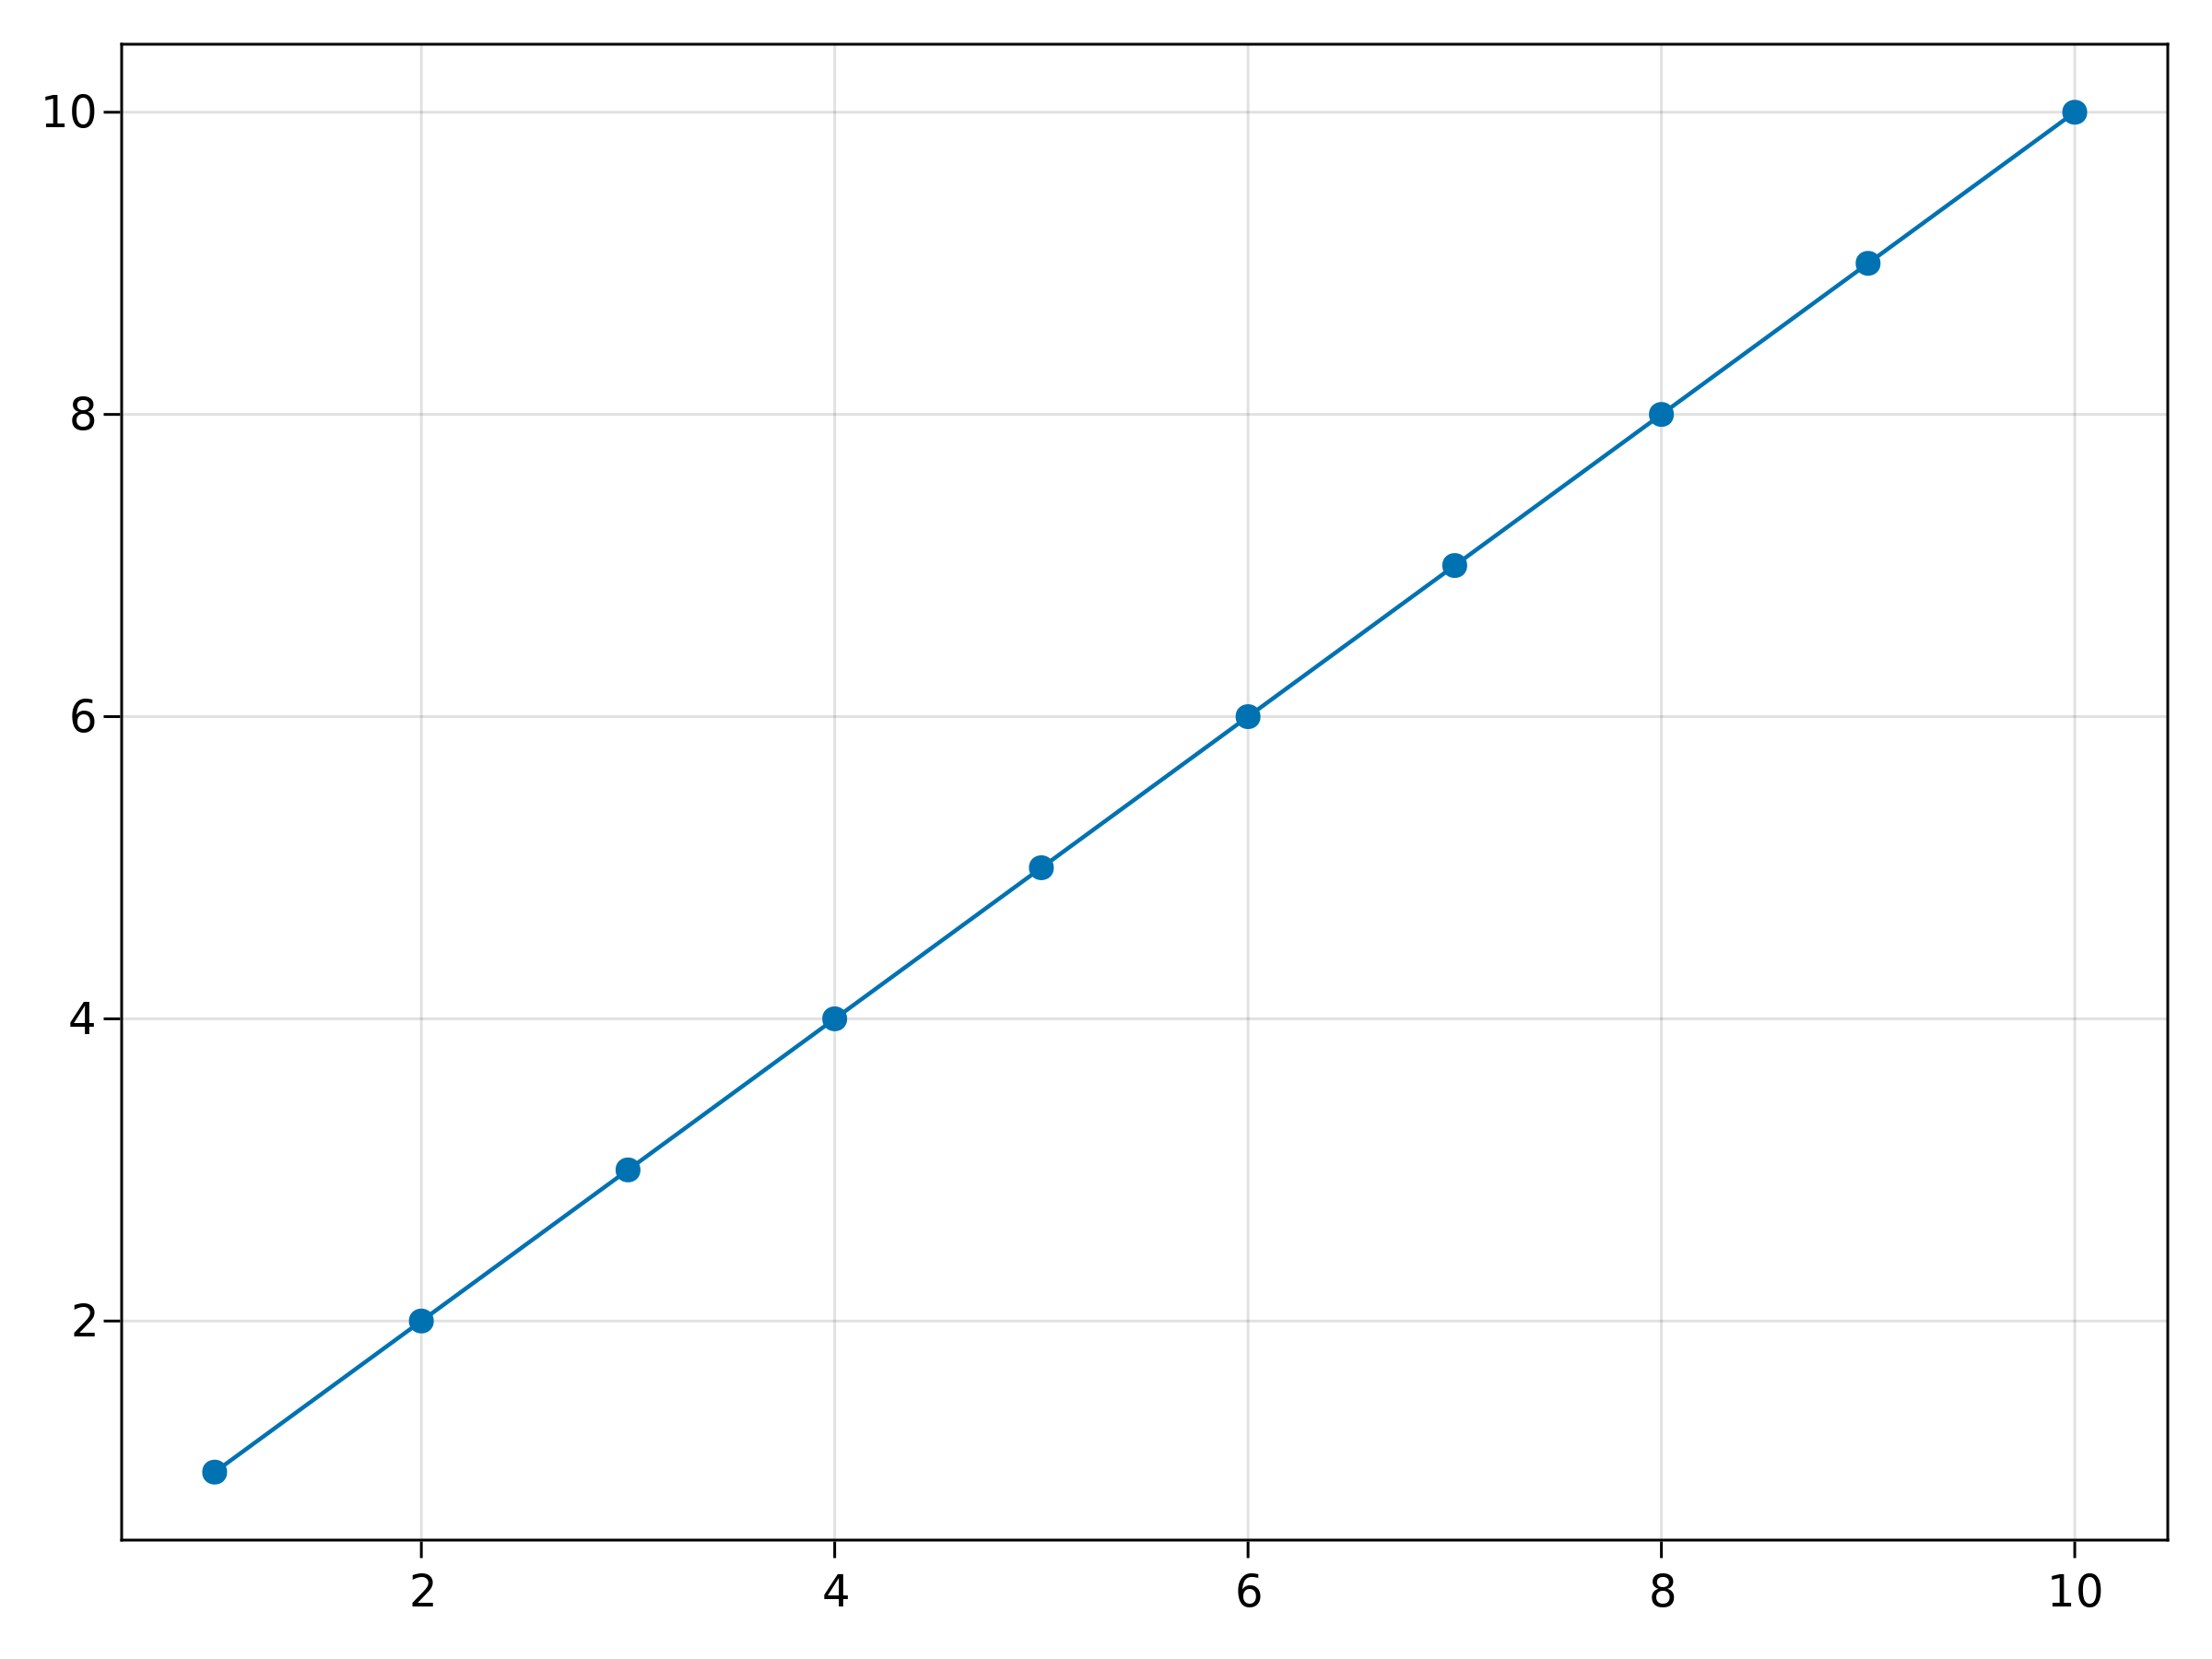
\includegraphics[width=0.6\textwidth,height=\textheight]{_build/im/firstplot.png}
\caption{First plot.}\label{fig:firstplot}
}
\end{figure}

Observe que o gráfico anterior é a saída padrão, que provavelmente
precisaremos ajustar usando nomes de eixo e rótulos.

Observe também que toda função de plotagem como
\passthrough{\lstinline!scatterlines!} cria e retorna novos objetos do
tipo \passthrough{\lstinline!Figure!}, \passthrough{\lstinline!Axis!} e
\passthrough{\lstinline!plot!} dentro de uma coleção chamada
\passthrough{\lstinline!FigureAxisPlot!}. Estes são conhecidos como os
métodos \emph{non-mutating} (imutáveis). Por outro lado, os métodos
\emph{mutating} (mutáveis, por exemplo,
\passthrough{\lstinline"scatterlines!"}, observe o
\passthrough{\lstinline"!"}) apenas retornam um objeto do tipo
\emph{plot} que pode ser anexado a um determinado
\passthrough{\lstinline!axis!} (eixo) ou à
\passthrough{\lstinline!current\_figure()!} (figura atual).

A próxima pergunta que se pode ter é: como mudo a cor ou o tipo de
marcador? Isso pode ser feito por meio de
\passthrough{\lstinline!attributes!} (atributos), o que faremos na
próxima seção.

\hypertarget{sec:datavisMakie_attributes}{%
\section{Atributos}\label{sec:datavisMakie_attributes}}

Um gráfico personalizado pode ser criado usando
\passthrough{\lstinline!attributes!} (atributos). Os atributos podem ser
definidos através de argumentos de palavras-chave. Uma lista de
\passthrough{\lstinline!atributos!} para cada objeto de plotagem pode
ser visualizada via:

\begin{lstlisting}[language=Julia]
fig, ax, pltobj = scatterlines(1:10)
pltobj.attributes
\end{lstlisting}

\begin{lstlisting}[language=Output]
Attributes with 15 entries:
  color => RGBA{Float32}(0.0,0.447059,0.698039,1.0)
  colormap => viridis
  colorrange => Automatic()
  cycle => [:color]
  inspectable => true
  linestyle => nothing
  linewidth => 1.5
  marker => Circle
  markercolor => Automatic()
  markercolormap => viridis
  markercolorrange => Automatic()
  markersize => 9
  model => Float32[1.0 0.0 0.0 0.0; 0.0 1.0 0.0 0.0; 0.0 0.0 1.0 0.0; 0.0 0.0 0.0 1.0]
  strokecolor => black
  strokewidth => 0
\end{lstlisting}

Ou como uma chamada de dicionário (\passthrough{\lstinline!Dict!}),
\passthrough{\lstinline!pltobject.attributes.attributes!}.

Pedir ajuda no \passthrough{\lstinline!REPL!} como
\passthrough{\lstinline!?lines!} ou
\passthrough{\lstinline!help(lines)!} para qualquer função de plotagem
mostrará seus atributos correspondentes acrescidos de uma breve
descrição de como usar essa função específica. Por exemplo, para
\passthrough{\lstinline!lines!}:

\begin{lstlisting}[language=Julia]
help(lines)
\end{lstlisting}

\begin{lstlisting}[language=Output]
  lines(positions)
  lines(x, y)
  lines(x, y, z)

  Creates a connected line plot for each element in (x, y, z), (x, y) or
  positions.

  │ Tip
  │
  │  You can separate segments by inserting NaNs.

  lines has the following function signatures:

    (Vector, Vector)
    (Vector, Vector, Vector)
    (Matrix)

  Available attributes for Lines are:

    color
    colormap
    colorrange
    cycle
    depth_shift
    diffuse
    inspectable
    linestyle
    linewidth
    nan_color
    overdraw
    shininess
    specular
    ssao
    transparency
    visible
\end{lstlisting}

Não apenas os objetos de tipo \emph{plot} têm atributos, como também os
objetos \passthrough{\lstinline!Axis!} (eixo) e
\passthrough{\lstinline!Figure!} (figura) os possuem. Por exemplo, para
figura, temos \passthrough{\lstinline!backgroundcolor!} (cor de fundo),
\passthrough{\lstinline!resolution!} (resolução),
\passthrough{\lstinline!font!} (fonte) e
\passthrough{\lstinline!fontsize!} (tamanho da fonte) e o
\passthrough{\lstinline!figure\_padding!} (preenchimento ou
passe-partout) que altera a quantidade de espaço ao redor do conteúdo da
figura, veja a área cinza no \emph{plot}, Figure (@ fig:custom\_plot).
Ele aceita como argumentos um número único para todos os lados, ou uma
tupla de quatro números para esquerda, direita, inferior e superior,
representando cada um dos lados.

\passthrough{\lstinline!Axis!} tem muito mais atributos, alguns deles
são \passthrough{\lstinline!backgroundcolor!} (cor de fundo),
\passthrough{\lstinline!xgridcolor!} (cor da grade do eixo x) e
\passthrough{\lstinline!title!} (título). Para uma lista completa basta
digitar \passthrough{\lstinline!help(Axis)!}.

Assim, para nosso próximo plot, designaremos vários atributos de uma só
vez, como segue:

\begin{lstlisting}[language=Julia]
lines(1:10, (1:10).^2; color=:black, linewidth=2, linestyle=:dash,
    figure=(; figure_padding=5, resolution=(600, 400), font="sans",
        backgroundcolor=:grey90, fontsize=16),
    axis=(; xlabel="x", ylabel="x²", title="title",
        xgridstyle=:dash, ygridstyle=:dash))
current_figure()
\end{lstlisting}

\begin{figure}
\hypertarget{fig:custom_plot}{%
\centering
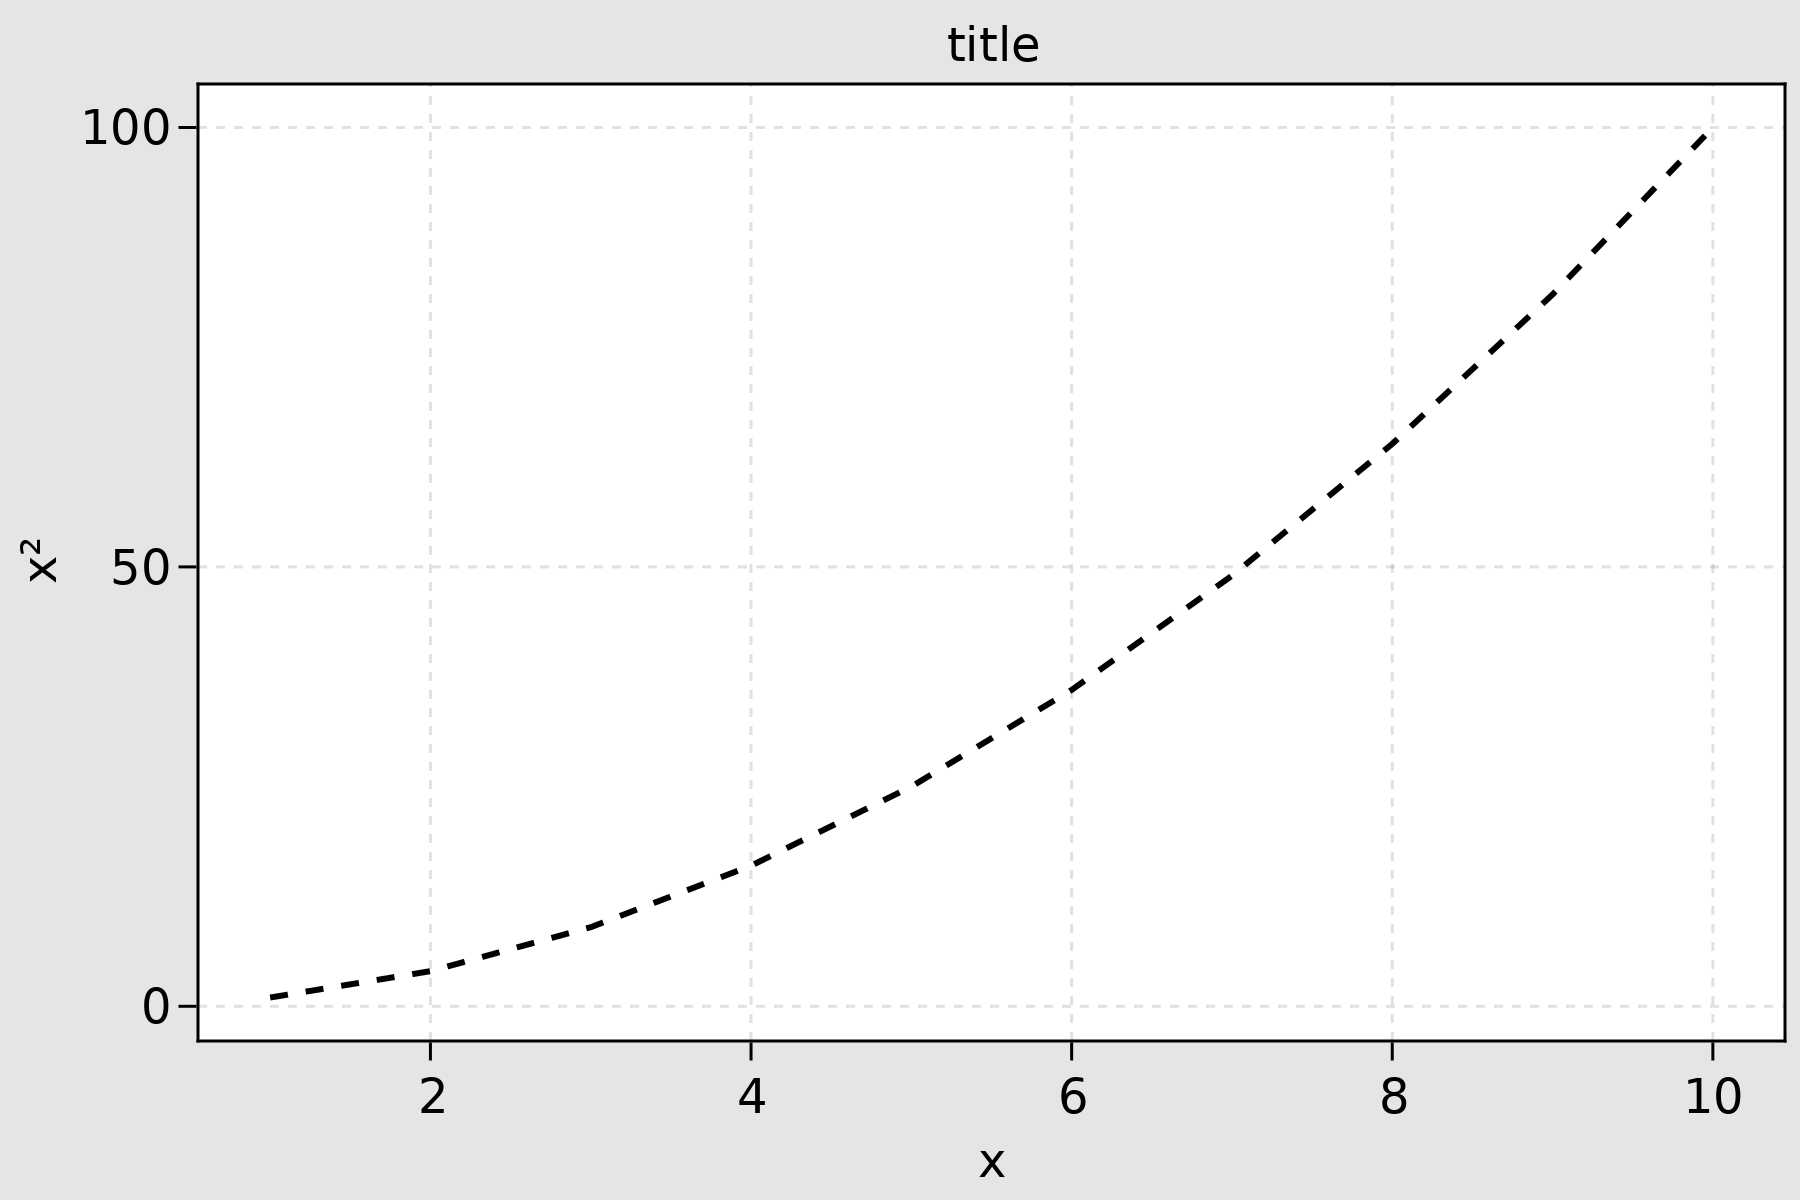
\includegraphics[width=0.6\textwidth,height=\textheight]{_build/im/custom_plot.png}
\caption{Custom plot.}\label{fig:custom_plot}
}
\end{figure}

Este exemplo já possui a maioria dos atributos que grande parte dos
usuários normalmente executará. Provavelmente, também seria bom ter uma
\passthrough{\lstinline!legend!} (legenda). O que fará mais sentido
quando utilizarmos mais de uma função de visualização. Então, vamos
\passthrough{\lstinline!append!} (acrescentar) outra mutação em nosso
\passthrough{\lstinline!plot object!} e adicionar as legendas
correspondentes chamando \passthrough{\lstinline!axislegend!}. A legenda
criada irá coletar todos os \passthrough{\lstinline!labels!} que você
pode ter passado para suas funções de plotagem e por padrão estará
localizada na posição superior direita. Para uma posição diferente, o
argumento \passthrough{\lstinline!position=:ct!} é chamado, onde
\passthrough{\lstinline!:ct!} significa que vamos colocar nosso rótulo
no `centro' e no `topo,' veja Figura Figure~\ref{fig:custom_plot_leg}:

\begin{lstlisting}[language=Julia]
lines(1:10, (1:10).^2; label="x²", linewidth=2, linestyle=nothing,
    figure=(; figure_padding=5, resolution=(600, 400), font="sans",
        backgroundcolor=:grey90, fontsize=16),
    axis=(; xlabel="x", title="title", xgridstyle=:dash,
        ygridstyle=:dash))
scatterlines!(1:10, (10:-1:1).^2; label="Reverse(x)²")
axislegend("legend"; position=:ct)
current_figure()
\end{lstlisting}

\begin{figure}
\hypertarget{fig:custom_plot_leg}{%
\centering
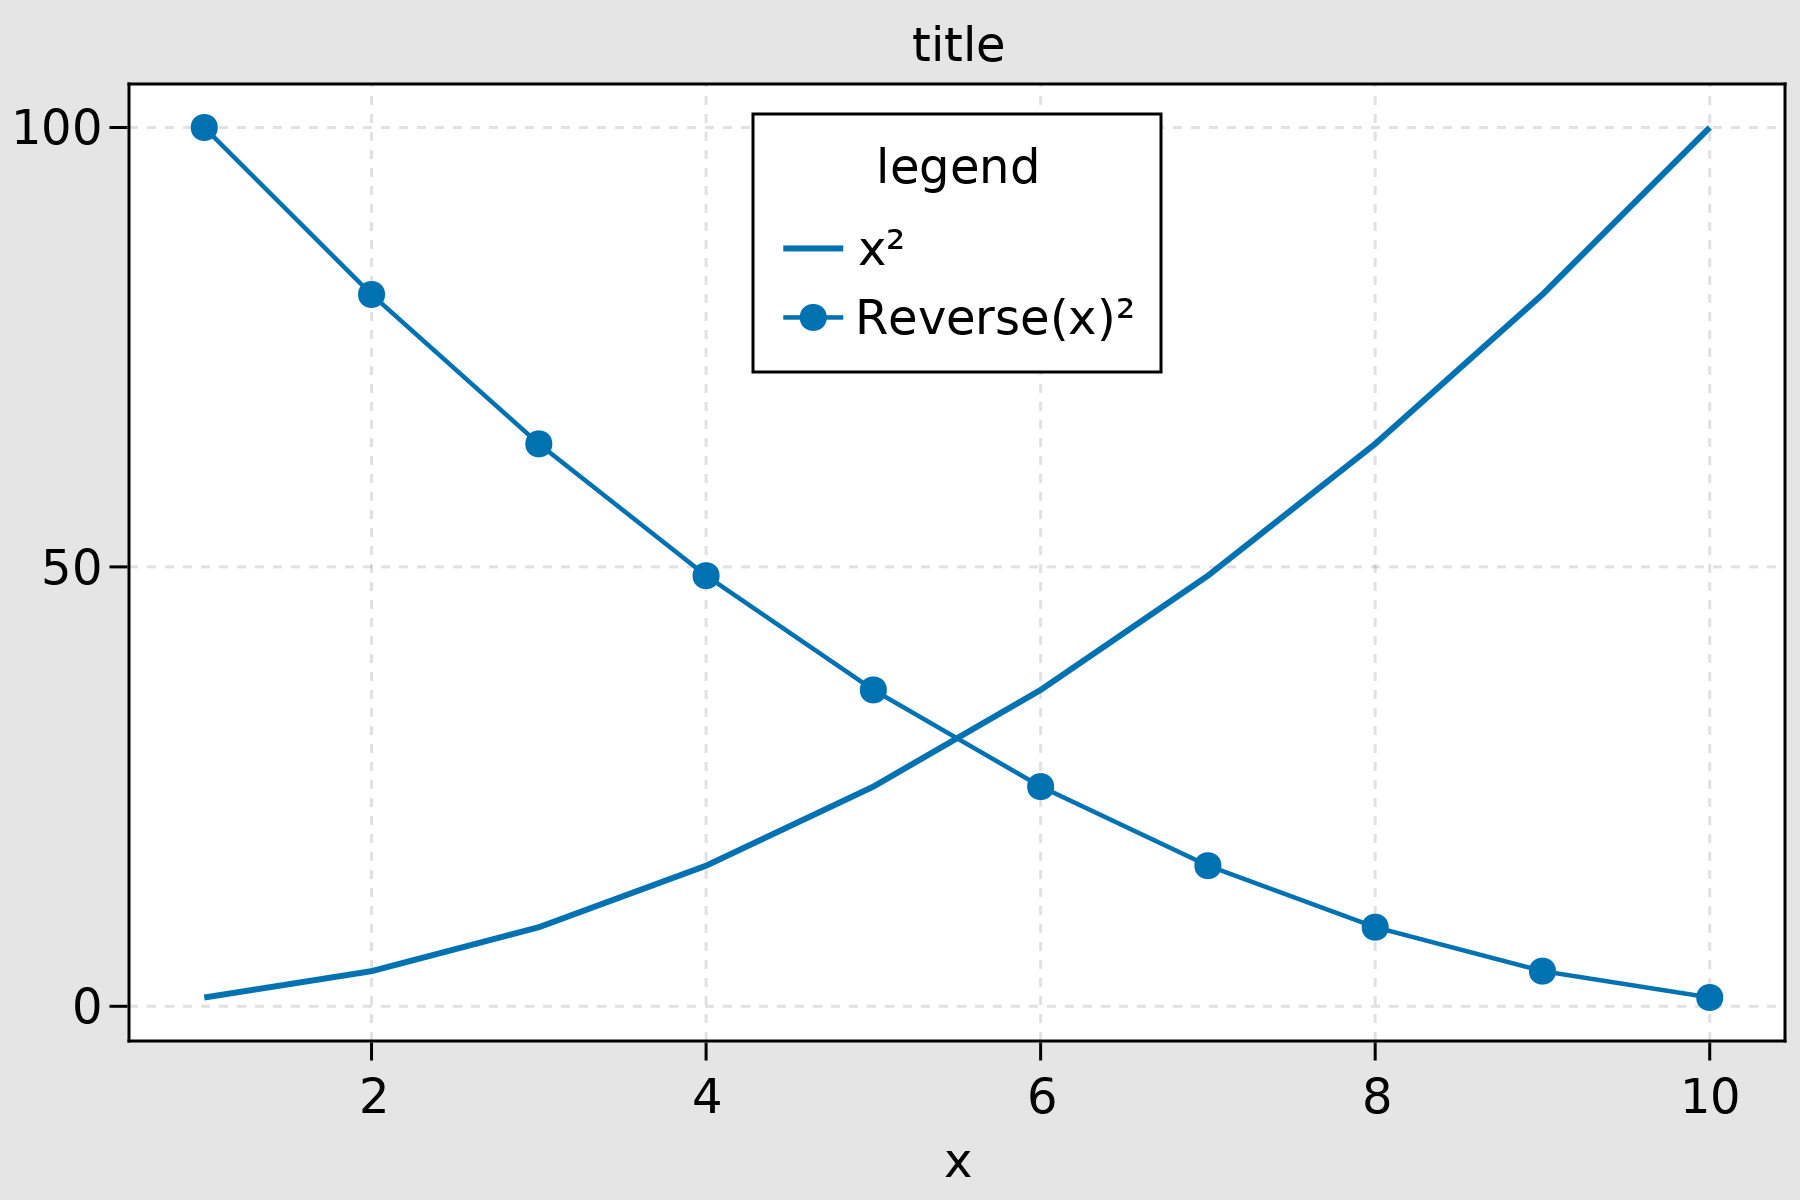
\includegraphics[width=0.6\textwidth,height=\textheight]{_build/im/custom_plot_leg.png}
\caption{Custom plot legend.}\label{fig:custom_plot_leg}
}
\end{figure}

Outras posições também estão disponíveis ao combinarmos
\passthrough{\lstinline!left(l), center(c), right(r)!} com
\passthrough{\lstinline!bottom(b), center(c), top(t)!}. Por exemplo,
para o topo superior esquerdo, use \passthrough{\lstinline!:lt!}.

No entanto, escrever essa quantidade de código apenas para duas linhas é
complicado. Portanto, se você planeja fazer muitos \emph{plots} com a
mesma estética geral, definir um tema é sempre melhor. Podemos fazer
isso com \passthrough{\lstinline"set\_theme!()"} como ilustrado pelo
exemplo abaixo.

A plotagem da figura anterior deve ter as novas configurações padrão
definidas por \passthrough{\lstinline"set\_theme!(kwargs)"}:

\begin{lstlisting}[language=Julia]
set_theme!(; resolution=(600, 400),
    backgroundcolor=(:orange, 0.5), fontsize=16, font="sans",
    Axis=(backgroundcolor=:grey90, xgridstyle=:dash, ygridstyle=:dash),
    Legend=(bgcolor=(:red, 0.2), framecolor=:dodgerblue))
lines(1:10, (1:10).^2; label="x²", linewidth=2, linestyle=nothing,
    axis=(; xlabel="x", title="title"))
scatterlines!(1:10, (10:-1:1).^2; label="Reverse(x)²")
axislegend("legend"; position=:ct)
current_figure()
set_theme!()
caption = "Set theme example."
\end{lstlisting}

\begin{figure}
\hypertarget{fig:setTheme}{%
\centering
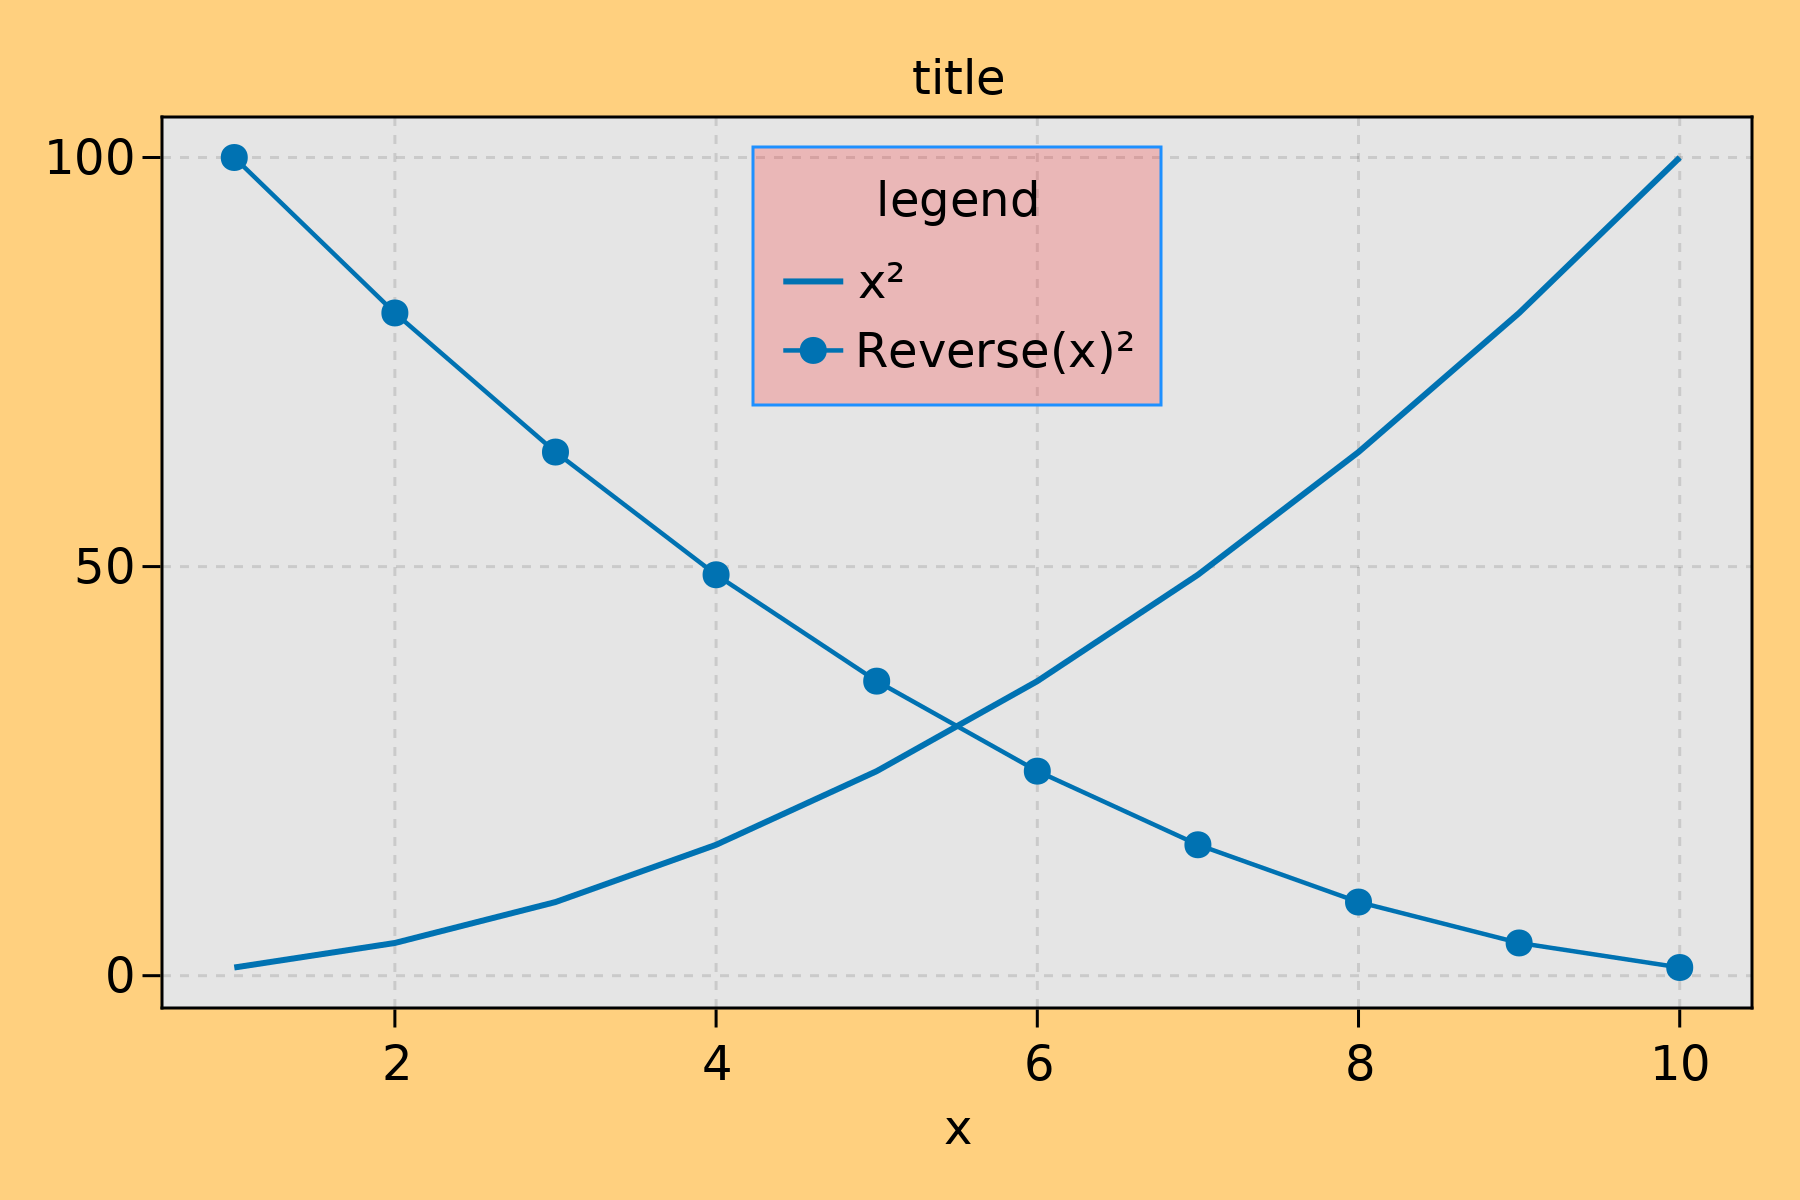
\includegraphics[width=0.6\textwidth,height=\textheight]{_build/im/setTheme.png}
\caption{Set theme example.}\label{fig:setTheme}
}
\end{figure}

Perceba que a última linha é \passthrough{\lstinline"set\_theme!()"},
que irá redefinir as configurações padrão do Makie. Para mais
\passthrough{\lstinline!themes!} por favor vá a
Section~\ref{sec:themes}.

Antes de passarmos para a próxima seção, vale a pena ver um exemplo onde
um \passthrough{\lstinline!array!} de atributos é passado de uma só vez
para uma função de plotagem. Para esse exemplo, usaremos a função de
plotagem \passthrough{\lstinline!scatter!} para fazer um gráfico de
dispersão.

Os dados para isso podem ser um \passthrough{\lstinline!array!} com 100
linhas e 3 colunas, aqui gerados aleatoriamente a partir de uma
distribuição normal. Aqui, a primeira coluna pode ser as posições no
eixo \passthrough{\lstinline!x!}, a segunda as posições em
\passthrough{\lstinline!y!} e a terceira um valor associado intrínseco
para cada ponto. O último pode ser representado em um gráfico por uma
`cor' diferente ou com um tamanho de marcador diferente. Em um gráfico
de dispersão podemos fazer os dois.

\begin{lstlisting}[language=Julia]
using Random: seed!
seed!(28)
xyvals = randn(100, 3)
xyvals[1:5, :]
\end{lstlisting}

\begin{lstlisting}[language=Output]
5×3 Matrix{Float64}:
  0.550992   1.27614    -0.659886
 -1.06587   -0.0287242   0.175126
 -0.721591  -1.84423     0.121052
  0.801169   0.862781   -0.221599
 -0.340826   0.0589894  -1.76359
\end{lstlisting}

A seguir, o \emph{plot} correspondente pode ser visto em
Figure~\ref{fig:bubble}:

\begin{lstlisting}[language=Julia]
fig, ax, pltobj = scatter(xyvals[:, 1], xyvals[:, 2]; color=xyvals[:, 3],
    label="Bubbles", colormap=:plasma, markersize=15 * abs.(xyvals[:, 3]),
    figure=(; resolution=(600, 400)), axis=(; aspect=DataAspect()))
limits!(-3, 3, -3, 3)
Legend(fig[1, 2], ax, valign=:top)
Colorbar(fig[1, 2], pltobj, height=Relative(3 / 4))
fig
caption = "Bubble plot."
\end{lstlisting}

\begin{figure}
\hypertarget{fig:bubble}{%
\centering
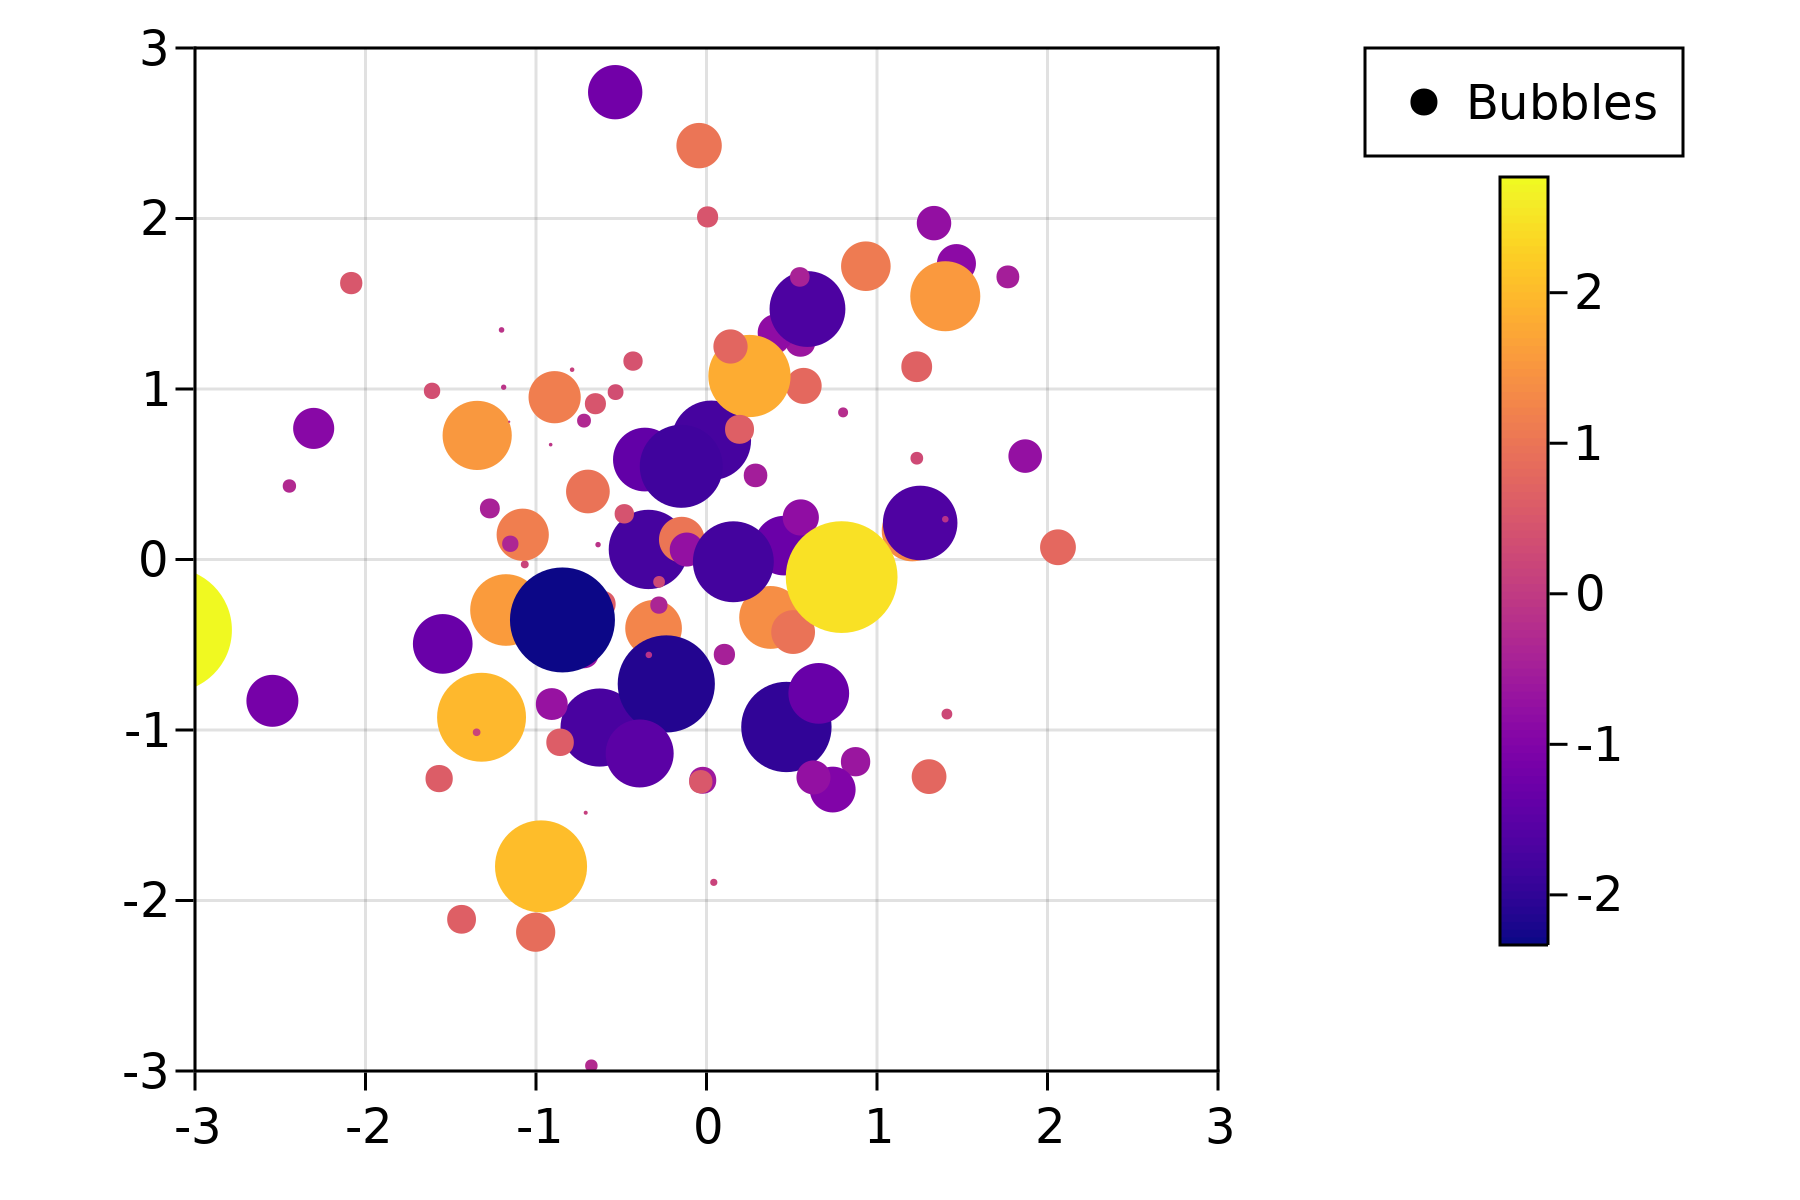
\includegraphics[width=0.6\textwidth,height=\textheight]{_build/im/bubble.png}
\caption{Bubble plot.}\label{fig:bubble}
}
\end{figure}

onde decompomos a tupla \passthrough{\lstinline!FigureAxisPlot!} em
\passthrough{\lstinline!fig, ax, pltobj!}, para podermos adicionar um
\passthrough{\lstinline!Legend!} e \passthrough{\lstinline!Colorbar!}
fora do objeto plotado. Vamos discutir opções de \emph{layout} mais
detalhadamente em in Section~\ref{sec:makie_layouts}.

Fizemos alguns exemplos básicos, mas ainda interessantes, para mostrar
como usar o \passthrough{\lstinline!Makie.jl!} e agora você deve estar
se perguntando: o que mais podemos fazer? Quais são todas as possíveis
funções de plotagem disponíveis em \passthrough{\lstinline!Makie.jl!}?
Para responder essa pergunta, contamos com uma \emph{cheat sheet} em
Figure~\ref{fig:cheat_sheet_cairomakie}. Isso funciona especialmente bem
com o \emph{backend} \passthrough{\lstinline!CairoMakie.jl!}.

\begin{figure}
\hypertarget{fig:cheat_sheet_cairomakie}{%
\centering
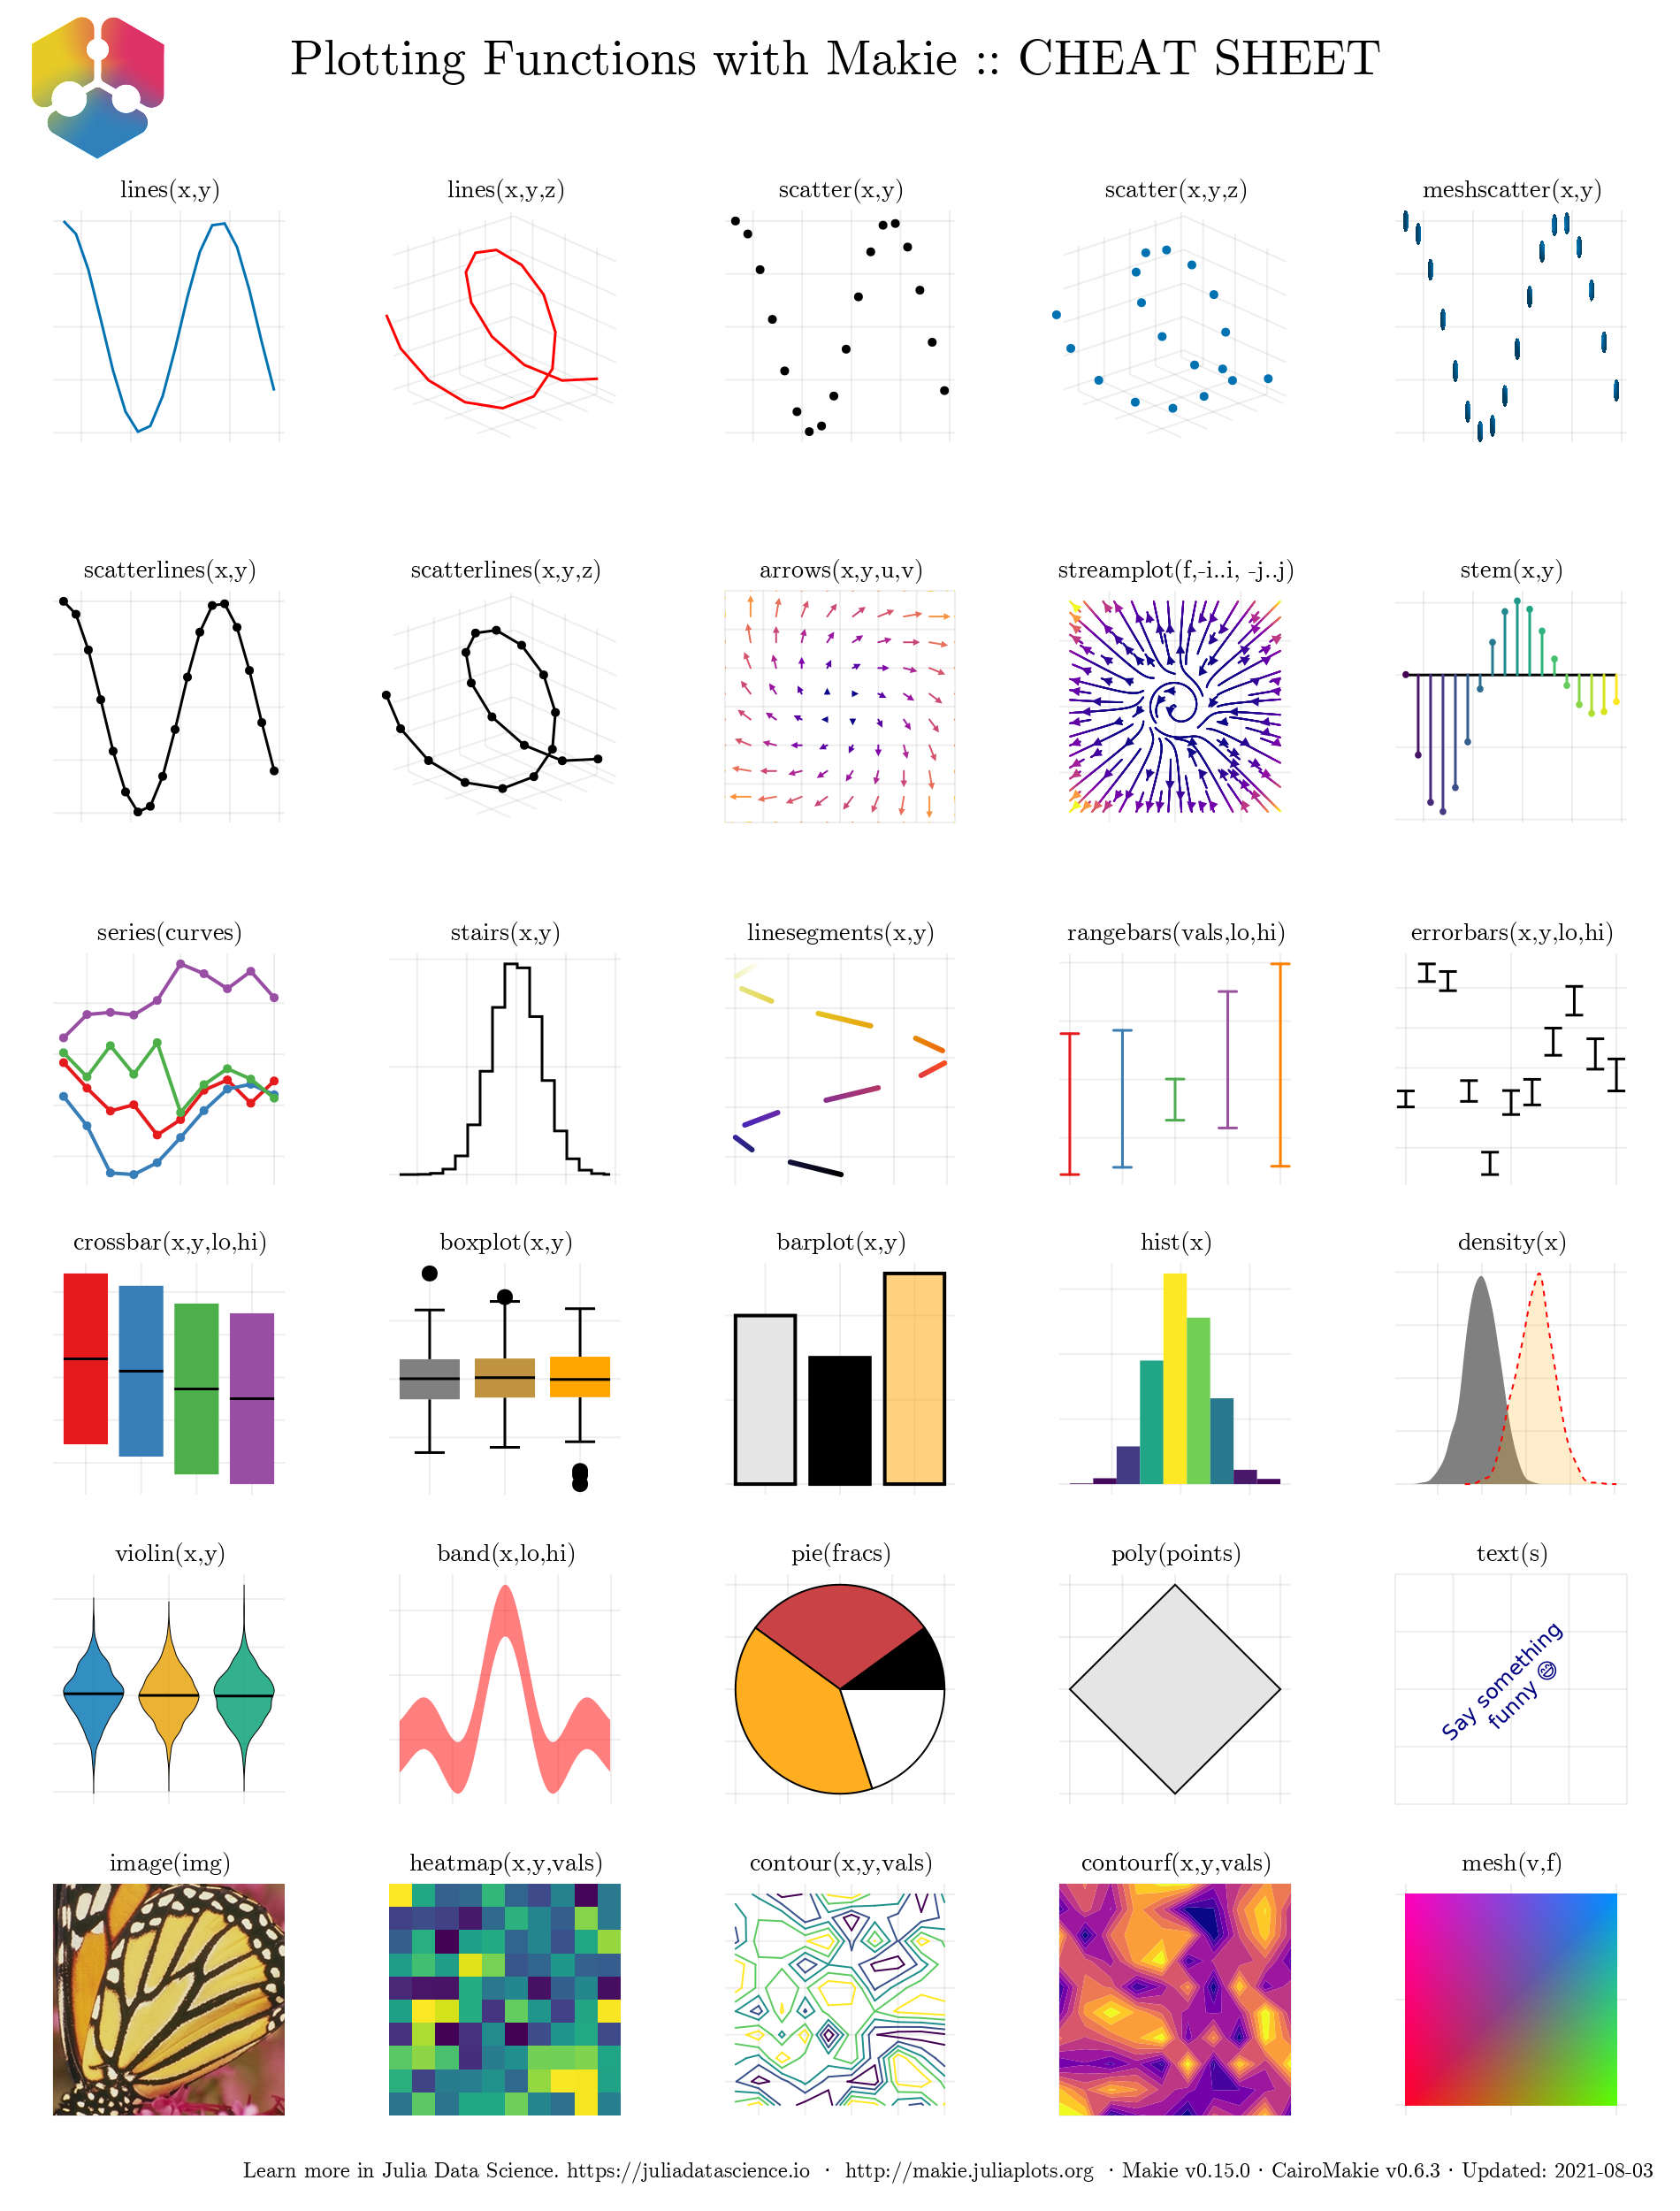
\includegraphics{images/makiePlottingFunctionsHide.png}
\caption{Funções de plotagem: Cheat Sheet. Saída dada por
Cairomakie.}\label{fig:cheat_sheet_cairomakie}
}
\end{figure}

Para completar, em Figure~\ref{fig:cheat_sheet_glmakie}, mostramos as
funções correspondentes \emph{cheat sheet} para
\passthrough{\lstinline!GLMakie.jl!}, que dão suporte principalmente
para plotagens 3D. Elas serão explicadas em detalhes em
Section~\ref{sec:glmakie}.

\begin{figure}
\hypertarget{fig:cheat_sheet_glmakie}{%
\centering
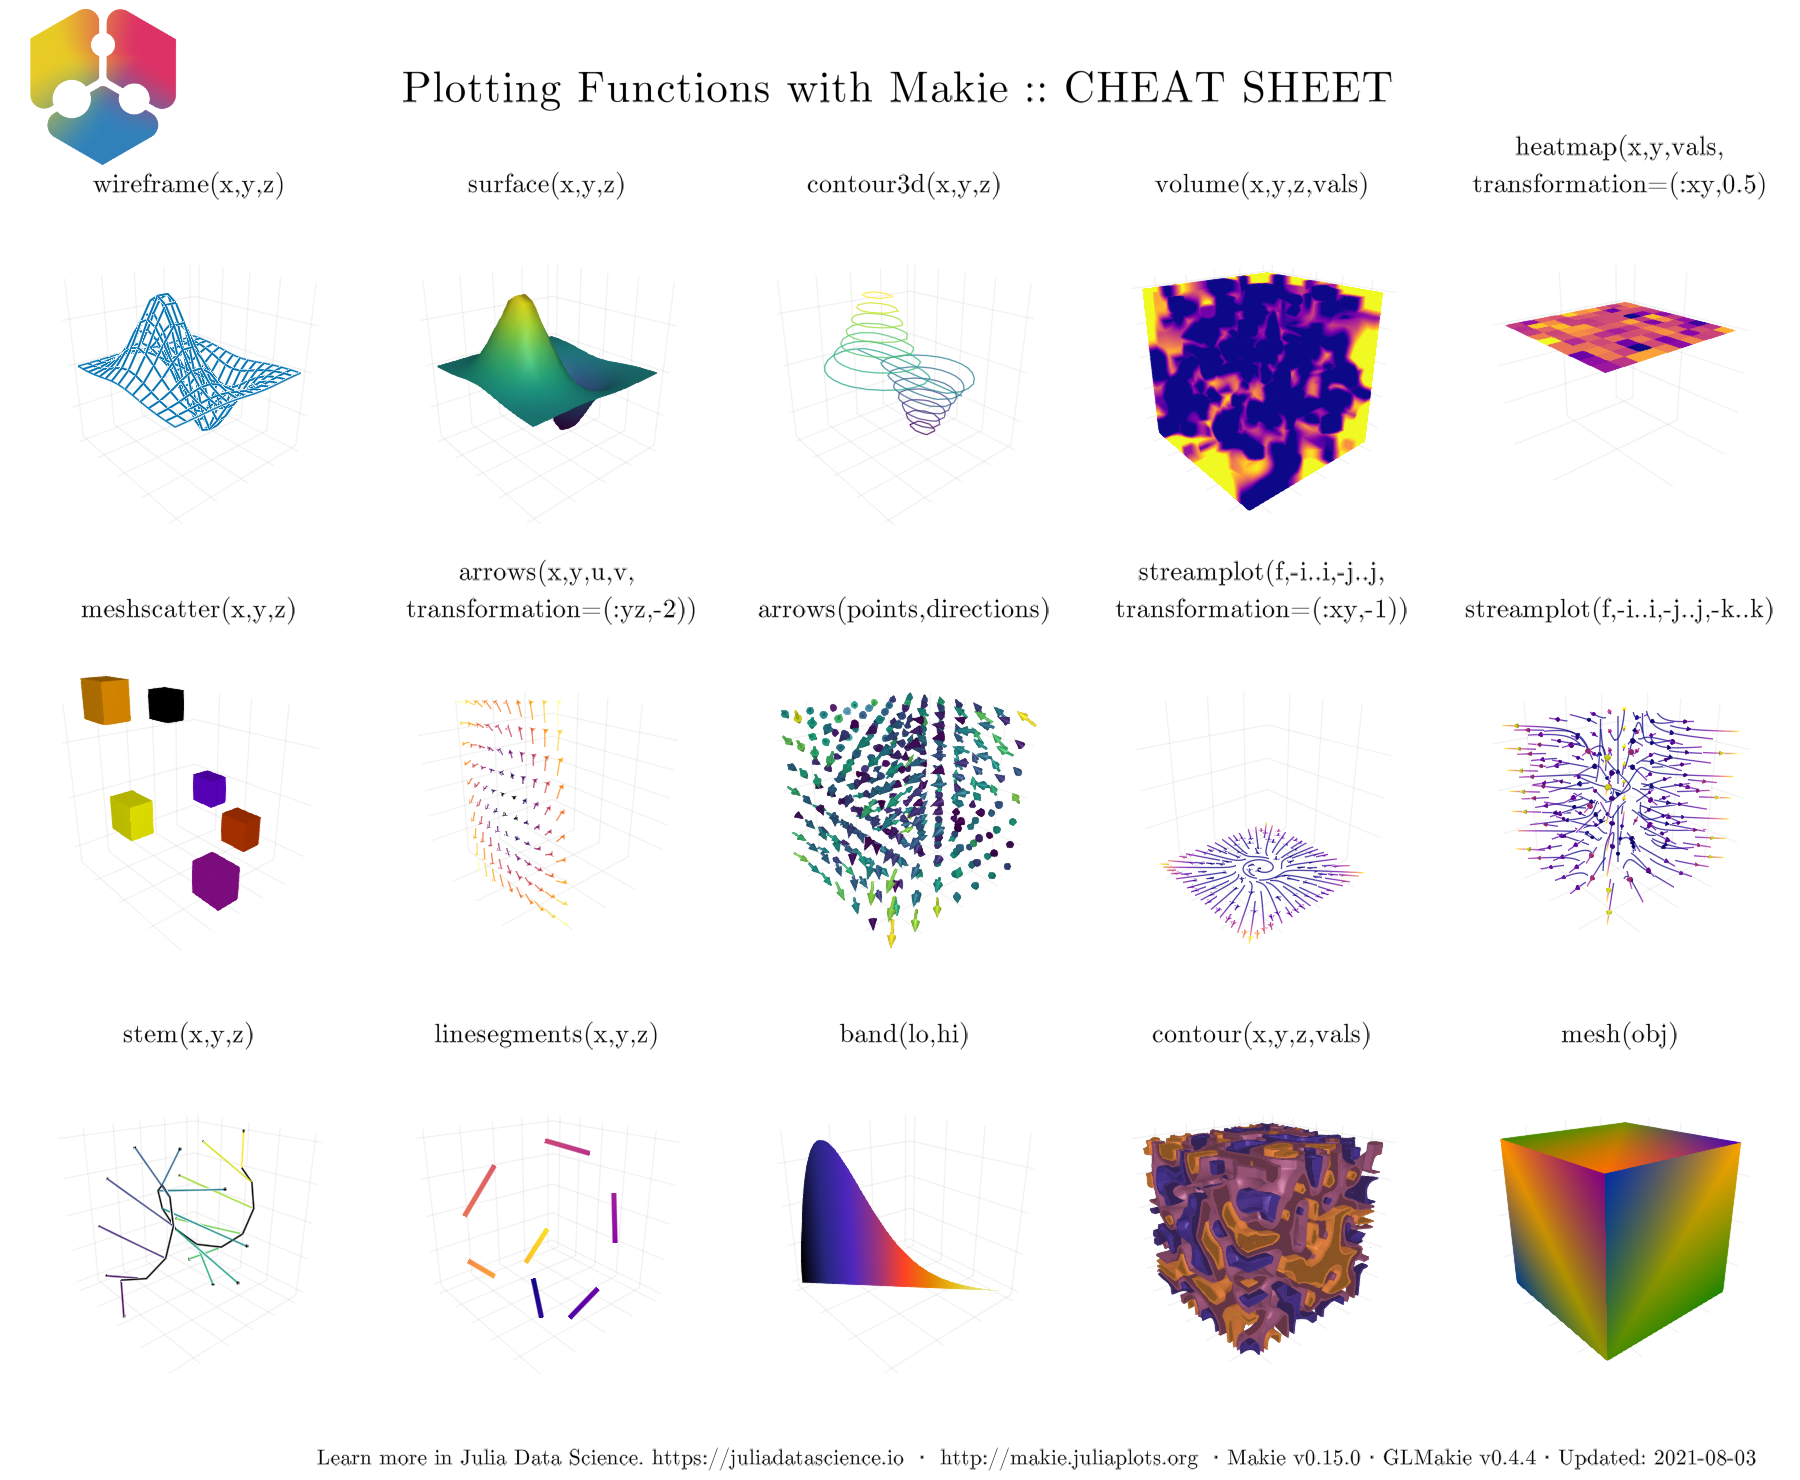
\includegraphics{images/GLMakiePlottingFunctionsHide.png}
\caption{Funções de plotagem: Cheat Sheet. Saída dada por
GLMakie.}\label{fig:cheat_sheet_glmakie}
}
\end{figure}

Agora que temos uma ideia de todas as coisas que podemos fazer, vamos
voltar e continuar com o básico. É hora de aprendermos a mudar a
aparência geral dos nossos \emph{plots}.

\hypertarget{sec:themes}{%
\section{Temas}\label{sec:themes}}

Existem várias maneiras de modificar a aparência geral de seus
\emph{plots}. Você pode usar um
\href{http://makie.juliaplots.org/stable/documentation/theming/predefined_themes/index.html}{tema
predefinido} ou seu próprio tema personalizado. Por exemplo, use um tema
escuro predefinido via
\passthrough{\lstinline!with\_theme(your\_plot\_function, theme\_dark())!}.
Ou construa o seu próprio com \passthrough{\lstinline!Theme(kwargs)!} ou
até mesmo atualize o que está ativo com
\passthrough{\lstinline"update\_theme!(kwargs)"}.

Você também pode fazer
\passthrough{\lstinline"set\_theme!(theme; kwargs...)"} para alterar o
tema do padrão atual para \passthrough{\lstinline!theme!} e substituir
ou adicionar atributos fornecidos por \passthrough{\lstinline!kwargs!}.
Se você fizer isso e quiser redefinir todas as configurações anteriores,
faça \passthrough{\lstinline"set\_theme!()"} sem argumentos. Veja os
exemplos a seguir, onde preparamos uma função de plotagem de teste com
características diferentes, de forma que a maioria dos atributos para
cada tema possa ser apreciada.

\begin{lstlisting}[language=Julia]
using Random: seed!
seed!(123)
y = cumsum(randn(6, 6), dims=2)
\end{lstlisting}

\begin{lstlisting}[language=Output]
6×6 Matrix{Float64}:
  0.808288   0.386519   0.355371   0.0365011  -0.0911358   1.8115
 -1.12207   -2.47766   -2.16183   -2.49928    -2.02981    -1.37017
 -1.10464   -1.03518   -3.19756   -1.18944    -2.71633    -3.80455
 -0.416993  -0.534315  -1.42439   -0.659362   -0.0592298   0.644529
  0.287588   1.50687    2.36111    2.54137     0.48751     0.630836
  0.229819   0.522733   0.864515   2.89343     2.06537     2.21375
\end{lstlisting}

Uma matrix de tamanho \passthrough{\lstinline!(20, 20)!} com entradas
aleatórias, para que possamos plotar um mapa de calor. O intervalo em
\(x\) e \(y\) também é especificado.

\begin{lstlisting}[language=Julia]
using Random: seed!
seed!(13)
xv = yv = LinRange(-3, 0.5, 20)
matrix = randn(20, 20)
matrix[1:6, 1:6] # first 6 rows and columns
\end{lstlisting}

\begin{lstlisting}[language=Output]
6×6 Matrix{Float64}:
 -0.271257   0.894952   0.728865  -0.293849   -0.449277   -0.0948871
 -0.193033  -0.421286  -0.455905  -0.0576092  -0.756621   -1.47419
 -0.123177   0.762254   0.773921  -0.38526    -0.0659695  -0.599284
 -1.47327    0.770122   1.20725    0.257913    0.111979    0.875439
 -1.82913   -0.603888   0.164083  -0.118504    1.46723     0.0948876
  1.09769    0.178207   0.110243  -0.543203    0.592245    0.328993
\end{lstlisting}

Portanto, nossa função de plotagem se parece com o seguinte:

\begin{lstlisting}[language=Julia]
function demo_themes(y, xv, yv, matrix)
    fig, _ = series(y; labels=["$i" for i = 1:6], markersize=10,
        color=:Set1, figure=(; resolution=(600, 300)),
        axis=(; xlabel="time (s)", ylabel="Amplitude",
            title="Measurements"))
    hmap = heatmap!(xv, yv, matrix; colormap=:plasma)
    limits!(-3.1, 8.5, -6, 5.1)
    axislegend("legend"; merge=true)
    Colorbar(fig[1, 2], hmap)
    fig
end
\end{lstlisting}

Observe que a função \passthrough{\lstinline!series!} foi usada para
plotar várias linhas e dispersões de uma só vez com seus rótulos
correspondentes. Além disso, um mapa de calor com sua barra de cores foi
incluído. Atualmente, existem dois temas escuros, um chamado
\passthrough{\lstinline!theme\_dark()!} e outro
\passthrough{\lstinline!theme\_black()!}:

\begin{lstlisting}[language=Julia]
with_theme(theme_dark()) do
    demo_themes(y, xv, yv, matrix)
end
with_theme(theme_black()) do
    demo_themes(y, xv, yv, matrix)
end
\end{lstlisting}

\begin{figure}
\hypertarget{fig:theme_dark}{%
\centering
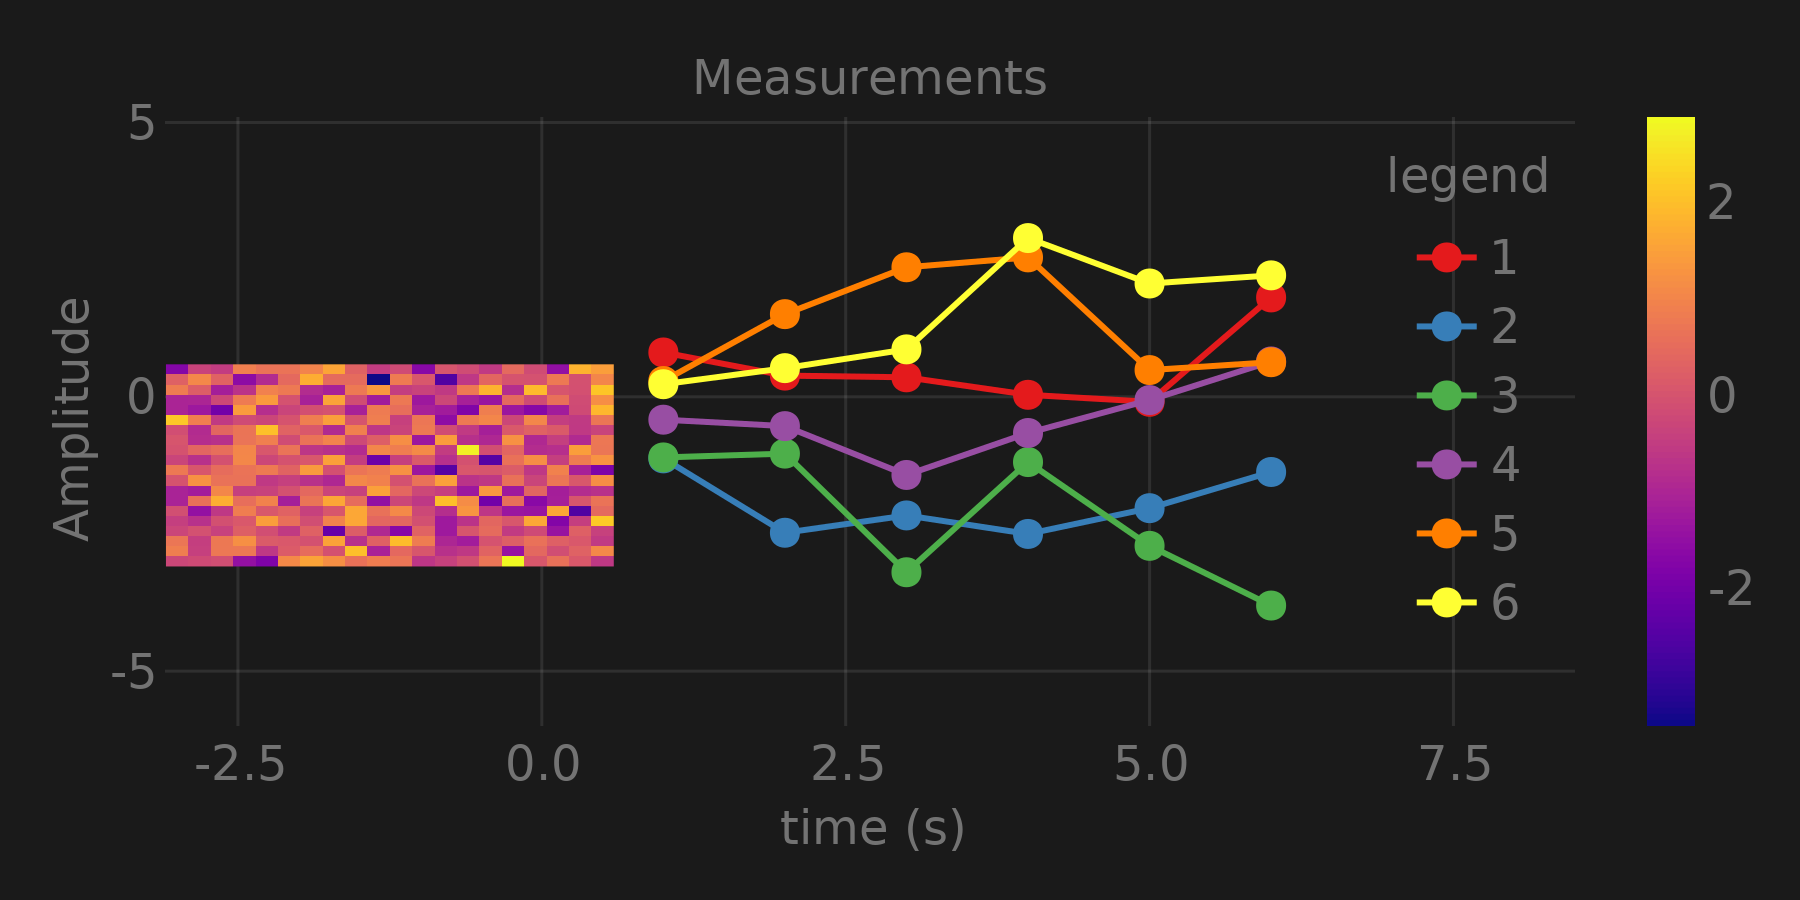
\includegraphics[width=0.6\textwidth,height=\textheight]{_build/im/theme_dark.png}
\caption{Theme dark.}\label{fig:theme_dark}
}
\end{figure}

\begin{figure}
\hypertarget{fig:theme_black}{%
\centering
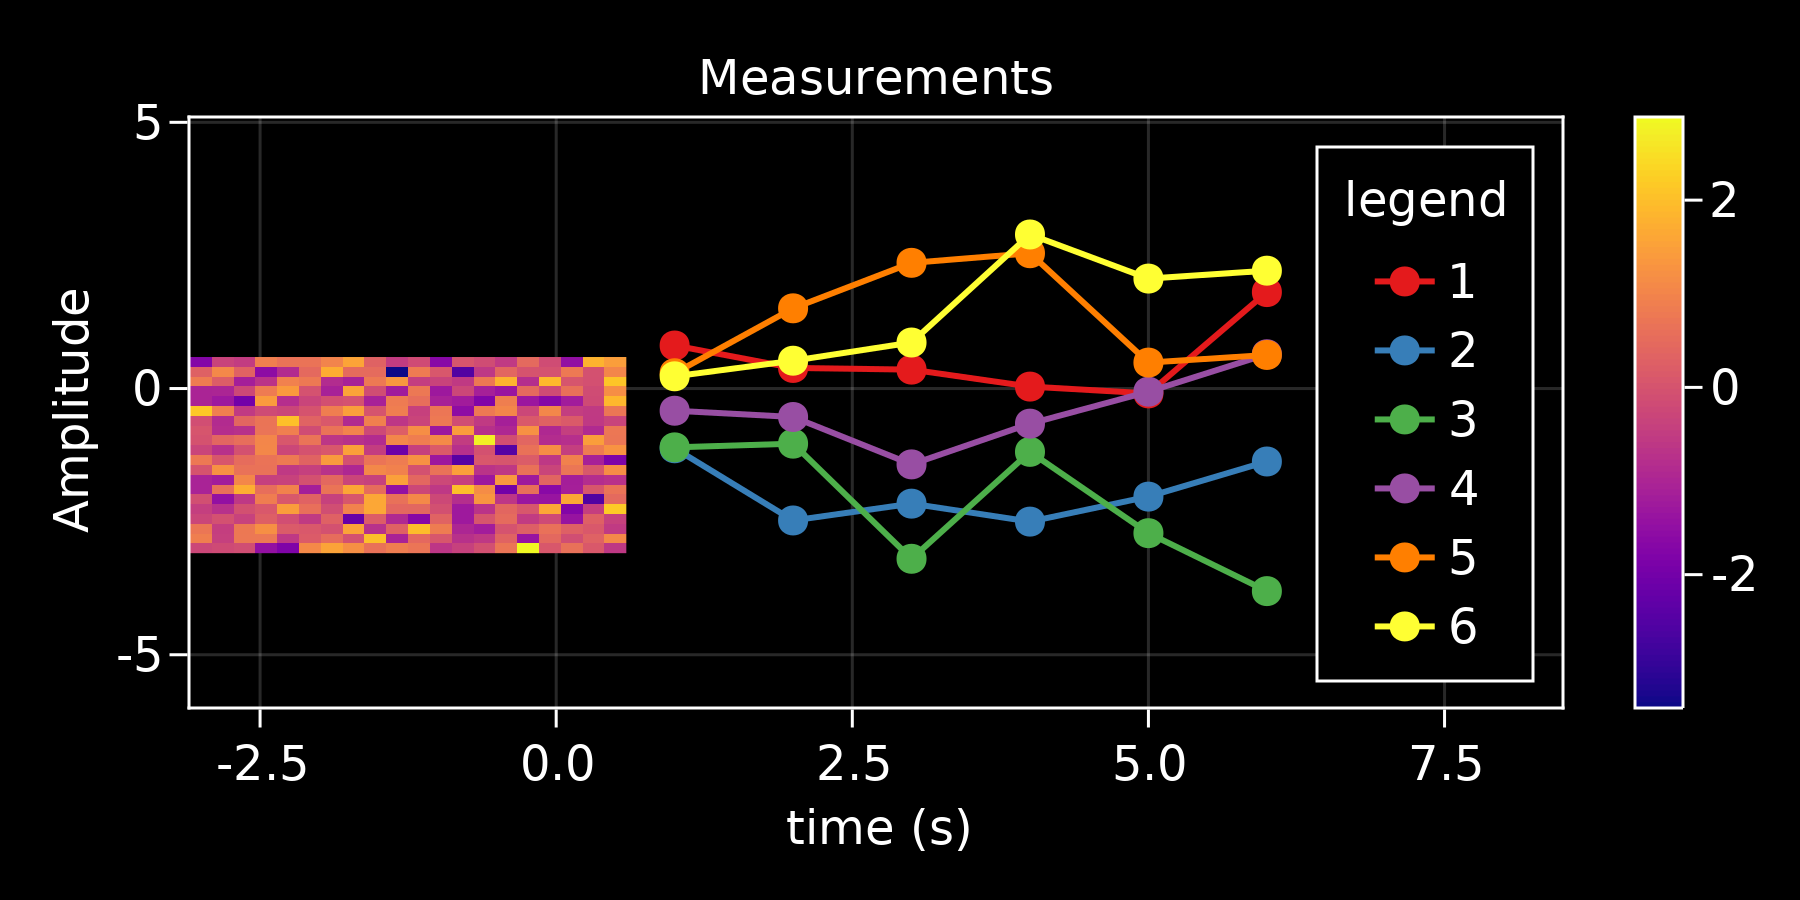
\includegraphics[width=0.6\textwidth,height=\textheight]{_build/im/theme_black.png}
\caption{Theme black.}\label{fig:theme_black}
}
\end{figure}

E mais três temas claros chamados,
\passthrough{\lstinline!theme\_ggplot2()!},
\passthrough{\lstinline!theme\_minimal()!} e
\passthrough{\lstinline!theme\_light()!}. Útil para \emph{plots} de tipo
de publicação mais padrão.

\begin{lstlisting}[language=Julia]
with_theme(theme_ggplot2()) do
    demo_themes(y, xv, yv, matrix)
end
with_theme(theme_minimal()) do
    demo_themes(y, xv, yv, matrix)
end
with_theme(theme_light()) do
    demo_themes(y, xv, yv, matrix)
end
\end{lstlisting}

\begin{figure}
\hypertarget{fig:theme_ggplot2}{%
\centering
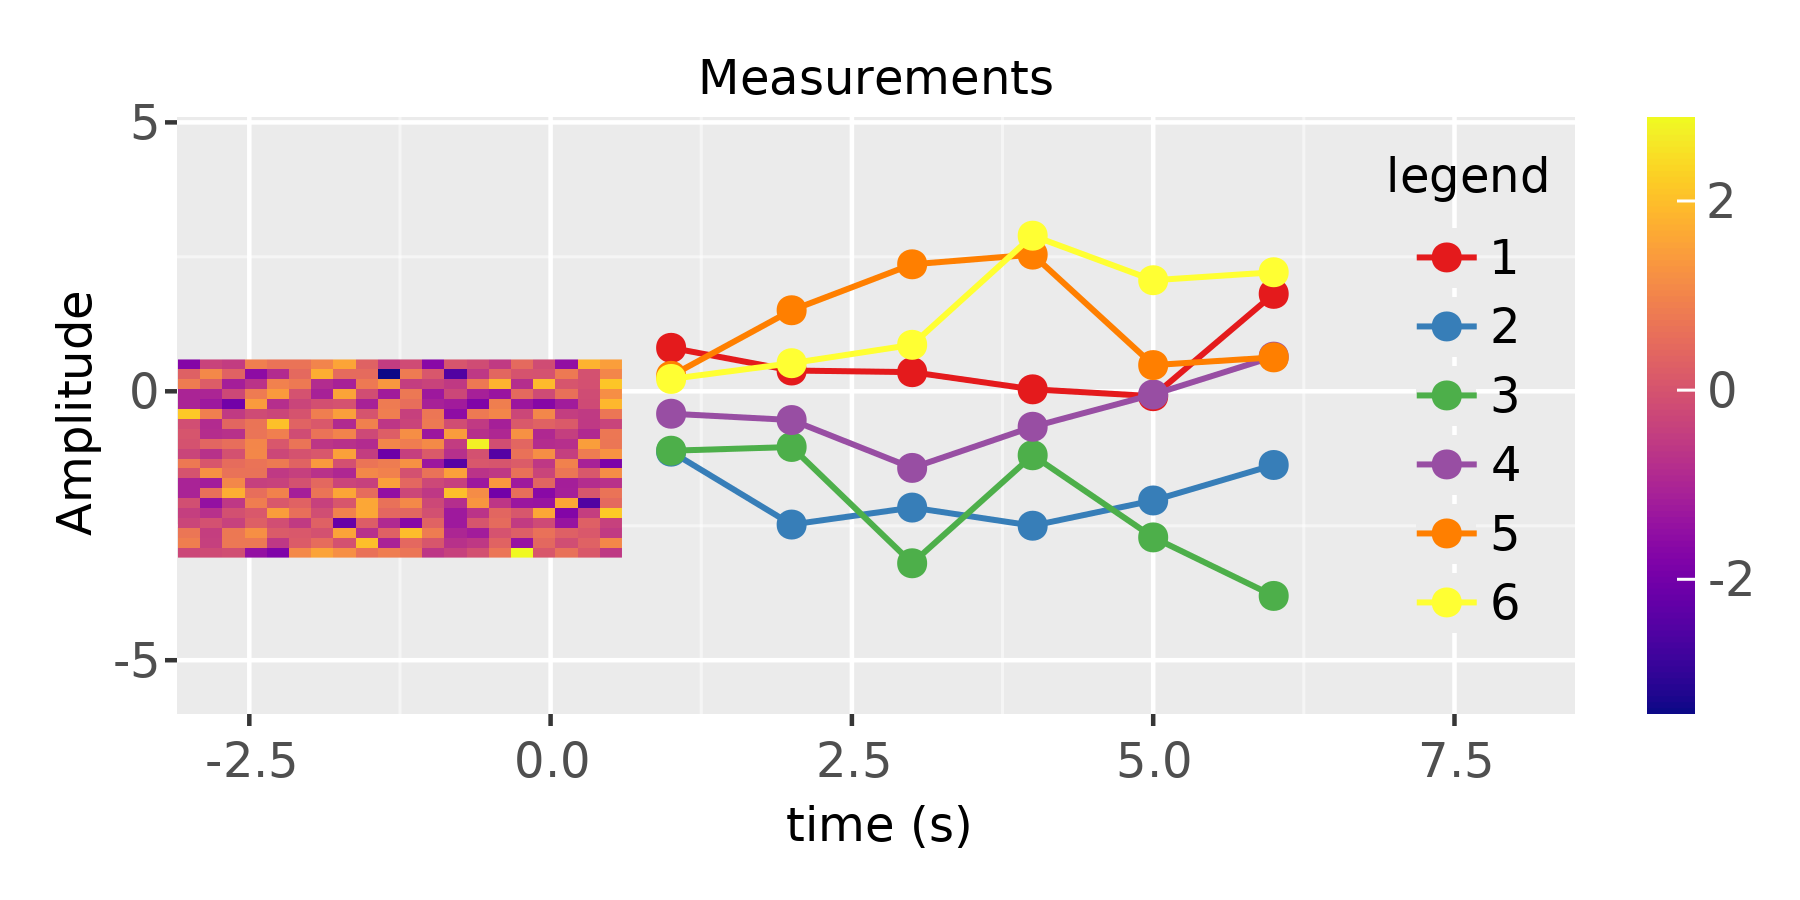
\includegraphics[width=0.6\textwidth,height=\textheight]{_build/im/theme_ggplot2.png}
\caption{Theme ggplot2.}\label{fig:theme_ggplot2}
}
\end{figure}

\begin{figure}
\hypertarget{fig:theme_minimal}{%
\centering
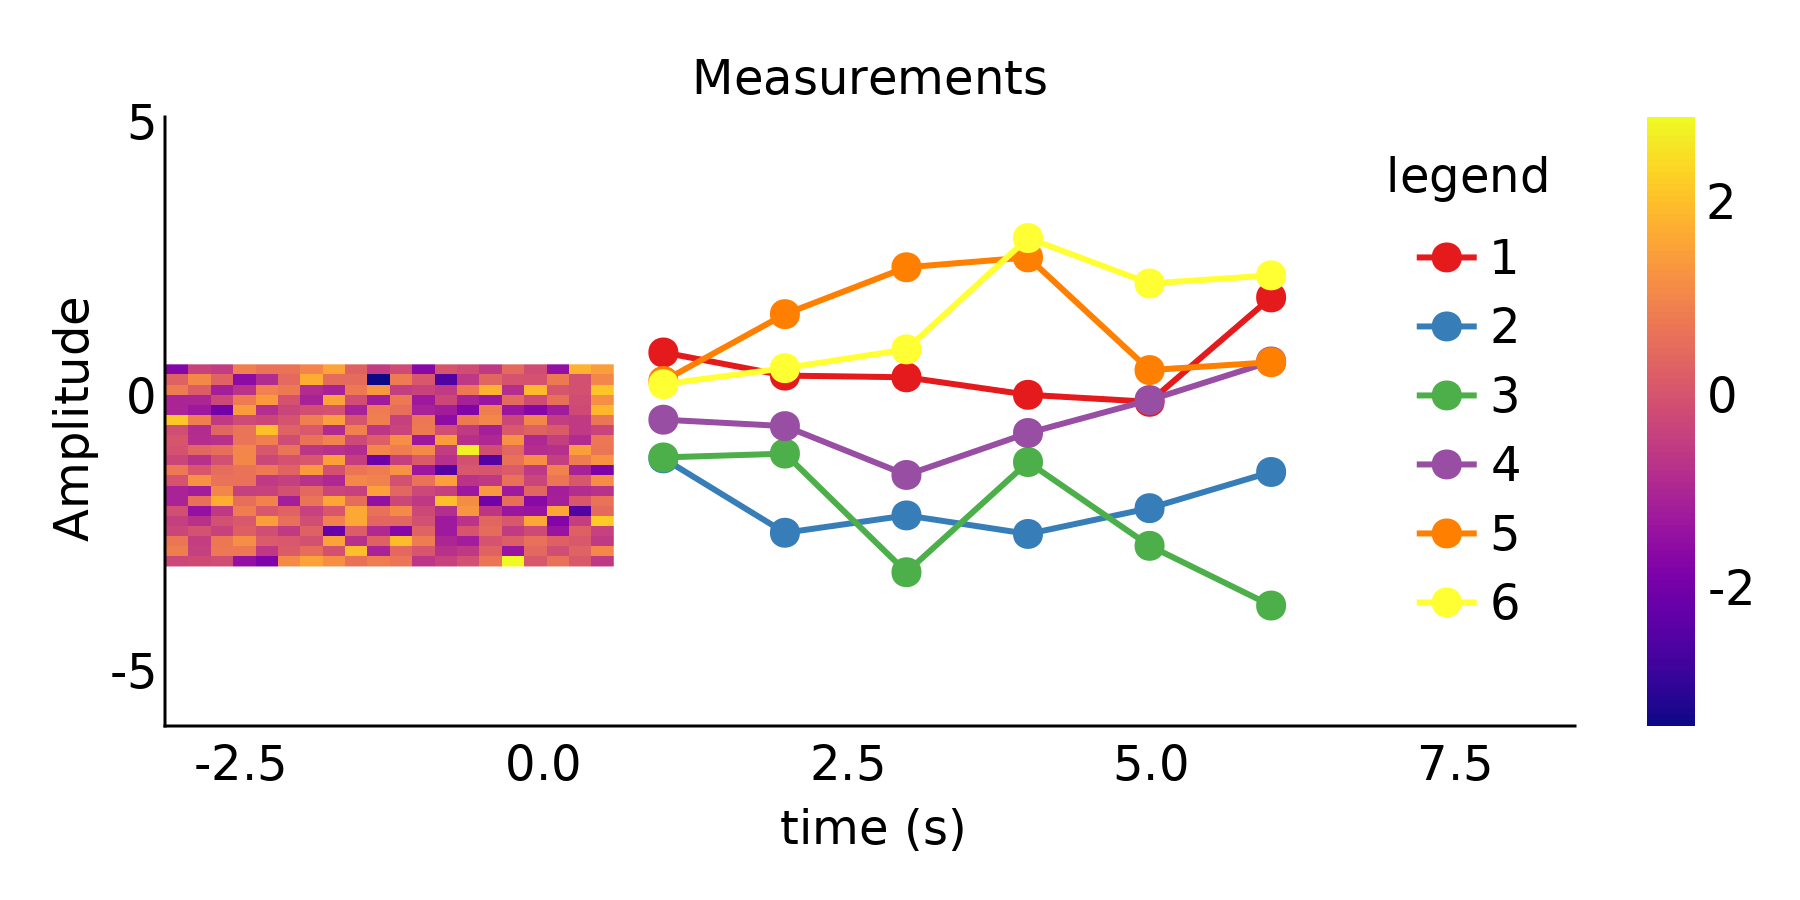
\includegraphics[width=0.6\textwidth,height=\textheight]{_build/im/theme_minimal.png}
\caption{Theme minimal.}\label{fig:theme_minimal}
}
\end{figure}

\begin{figure}
\hypertarget{fig:theme_light}{%
\centering
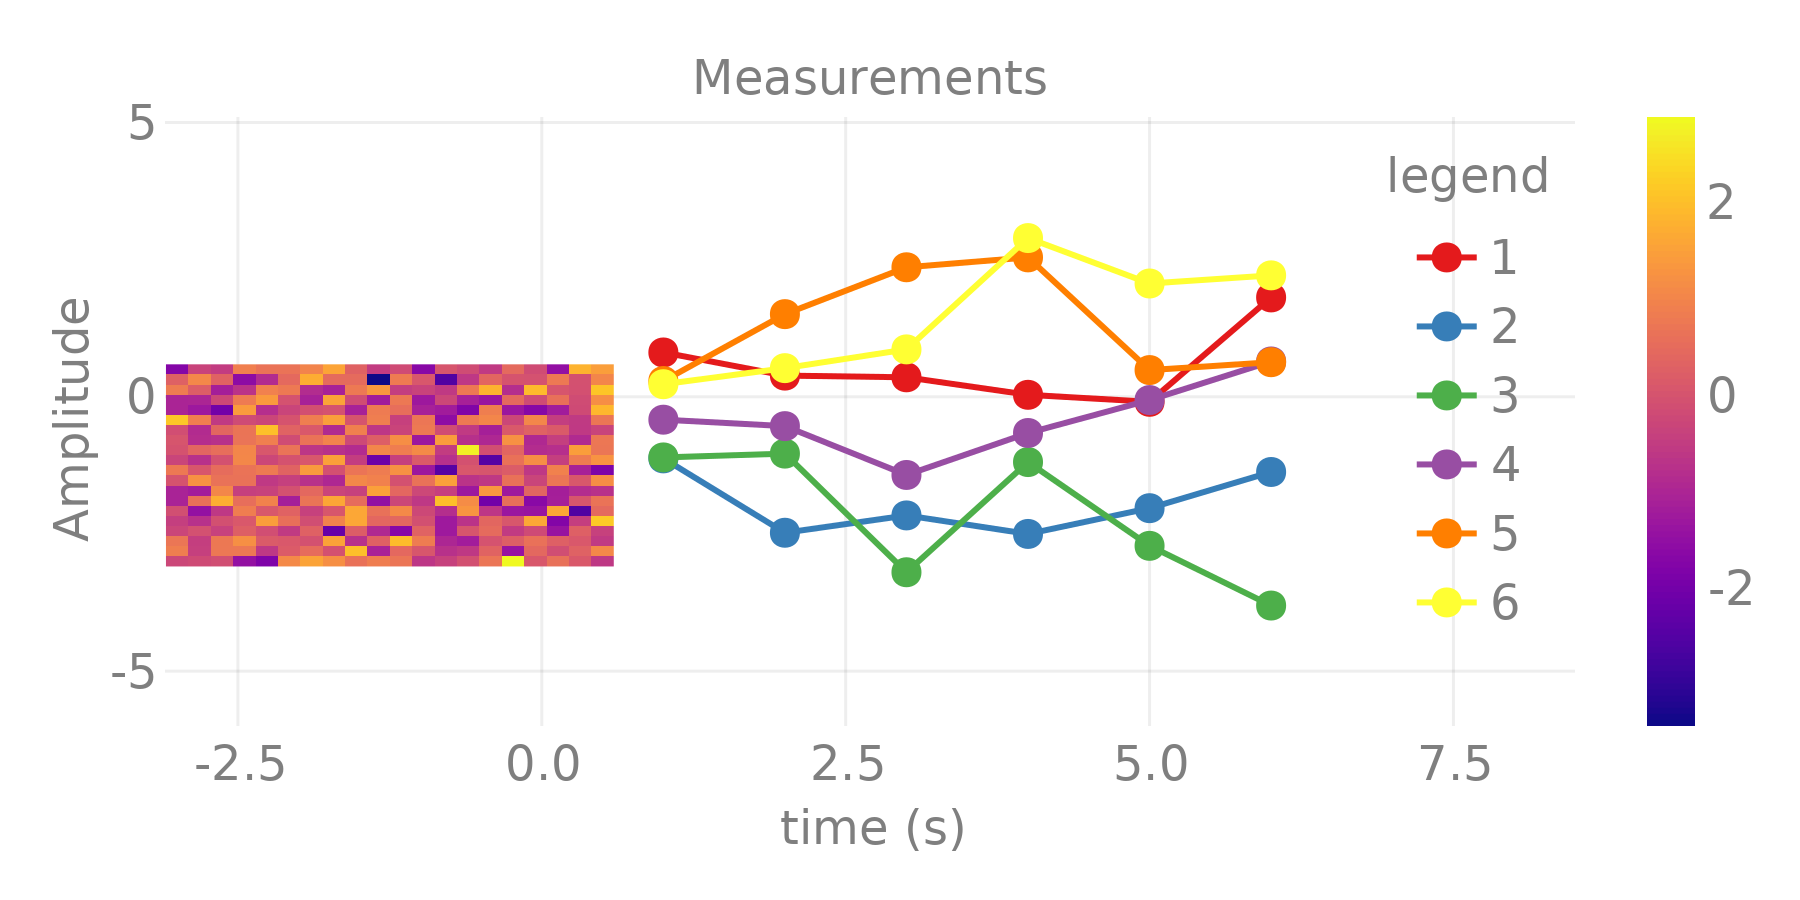
\includegraphics[width=0.6\textwidth,height=\textheight]{_build/im/theme_light.png}
\caption{Theme light.}\label{fig:theme_light}
}
\end{figure}

Outra alternativa é definir um \passthrough{\lstinline!Theme!} fazendo
\passthrough{\lstinline!with\_theme(your\_plot, your\_theme())!}. Por
exemplo, o tema a seguir pode ser uma versão simples para um modelo de
qualidade de publicação:

\begin{lstlisting}[language=Julia]
publication_theme() = Theme(
    fontsize=16, font="CMU Serif",
    Axis=(xlabelsize=20, xgridstyle=:dash, ygridstyle=:dash,
        xtickalign=1, ytickalign=1, yticksize=10, xticksize=10,
        xlabelpadding=-5, xlabel="x", ylabel="y"),
    Legend=(framecolor=(:black, 0.5), bgcolor=(:white, 0.5)),
    Colorbar=(ticksize=16, tickalign=1, spinewidth=0.5),
)
\end{lstlisting}

Que, por simplicidade, usamos para plotar
\passthrough{\lstinline!scatterlines!} e um
\passthrough{\lstinline!heatmap!}.

\begin{lstlisting}[language=Julia]
function plot_with_legend_and_colorbar()
    fig, ax, _ = scatterlines(1:10; label="line")
    hm = heatmap!(ax, LinRange(6, 9, 15), LinRange(2, 5, 15), randn(15, 15);
        colormap=:Spectral_11)
    axislegend("legend"; position=:lt)
    Colorbar(fig[1, 2], hm, label="values")
    ax.title = "my custom theme"
    fig
end
\end{lstlisting}

Então, usando o \passthrough{\lstinline!Theme!} definido anteriormente,
a saída é mostrada na Figura
(Figure~\ref{fig:plot_with_legend_and_colorbar}).

\begin{lstlisting}[language=Julia]
with_theme(plot_with_legend_and_colorbar, publication_theme())
\end{lstlisting}

\begin{figure}
\hypertarget{fig:plot_with_legend_and_colorbar}{%
\centering
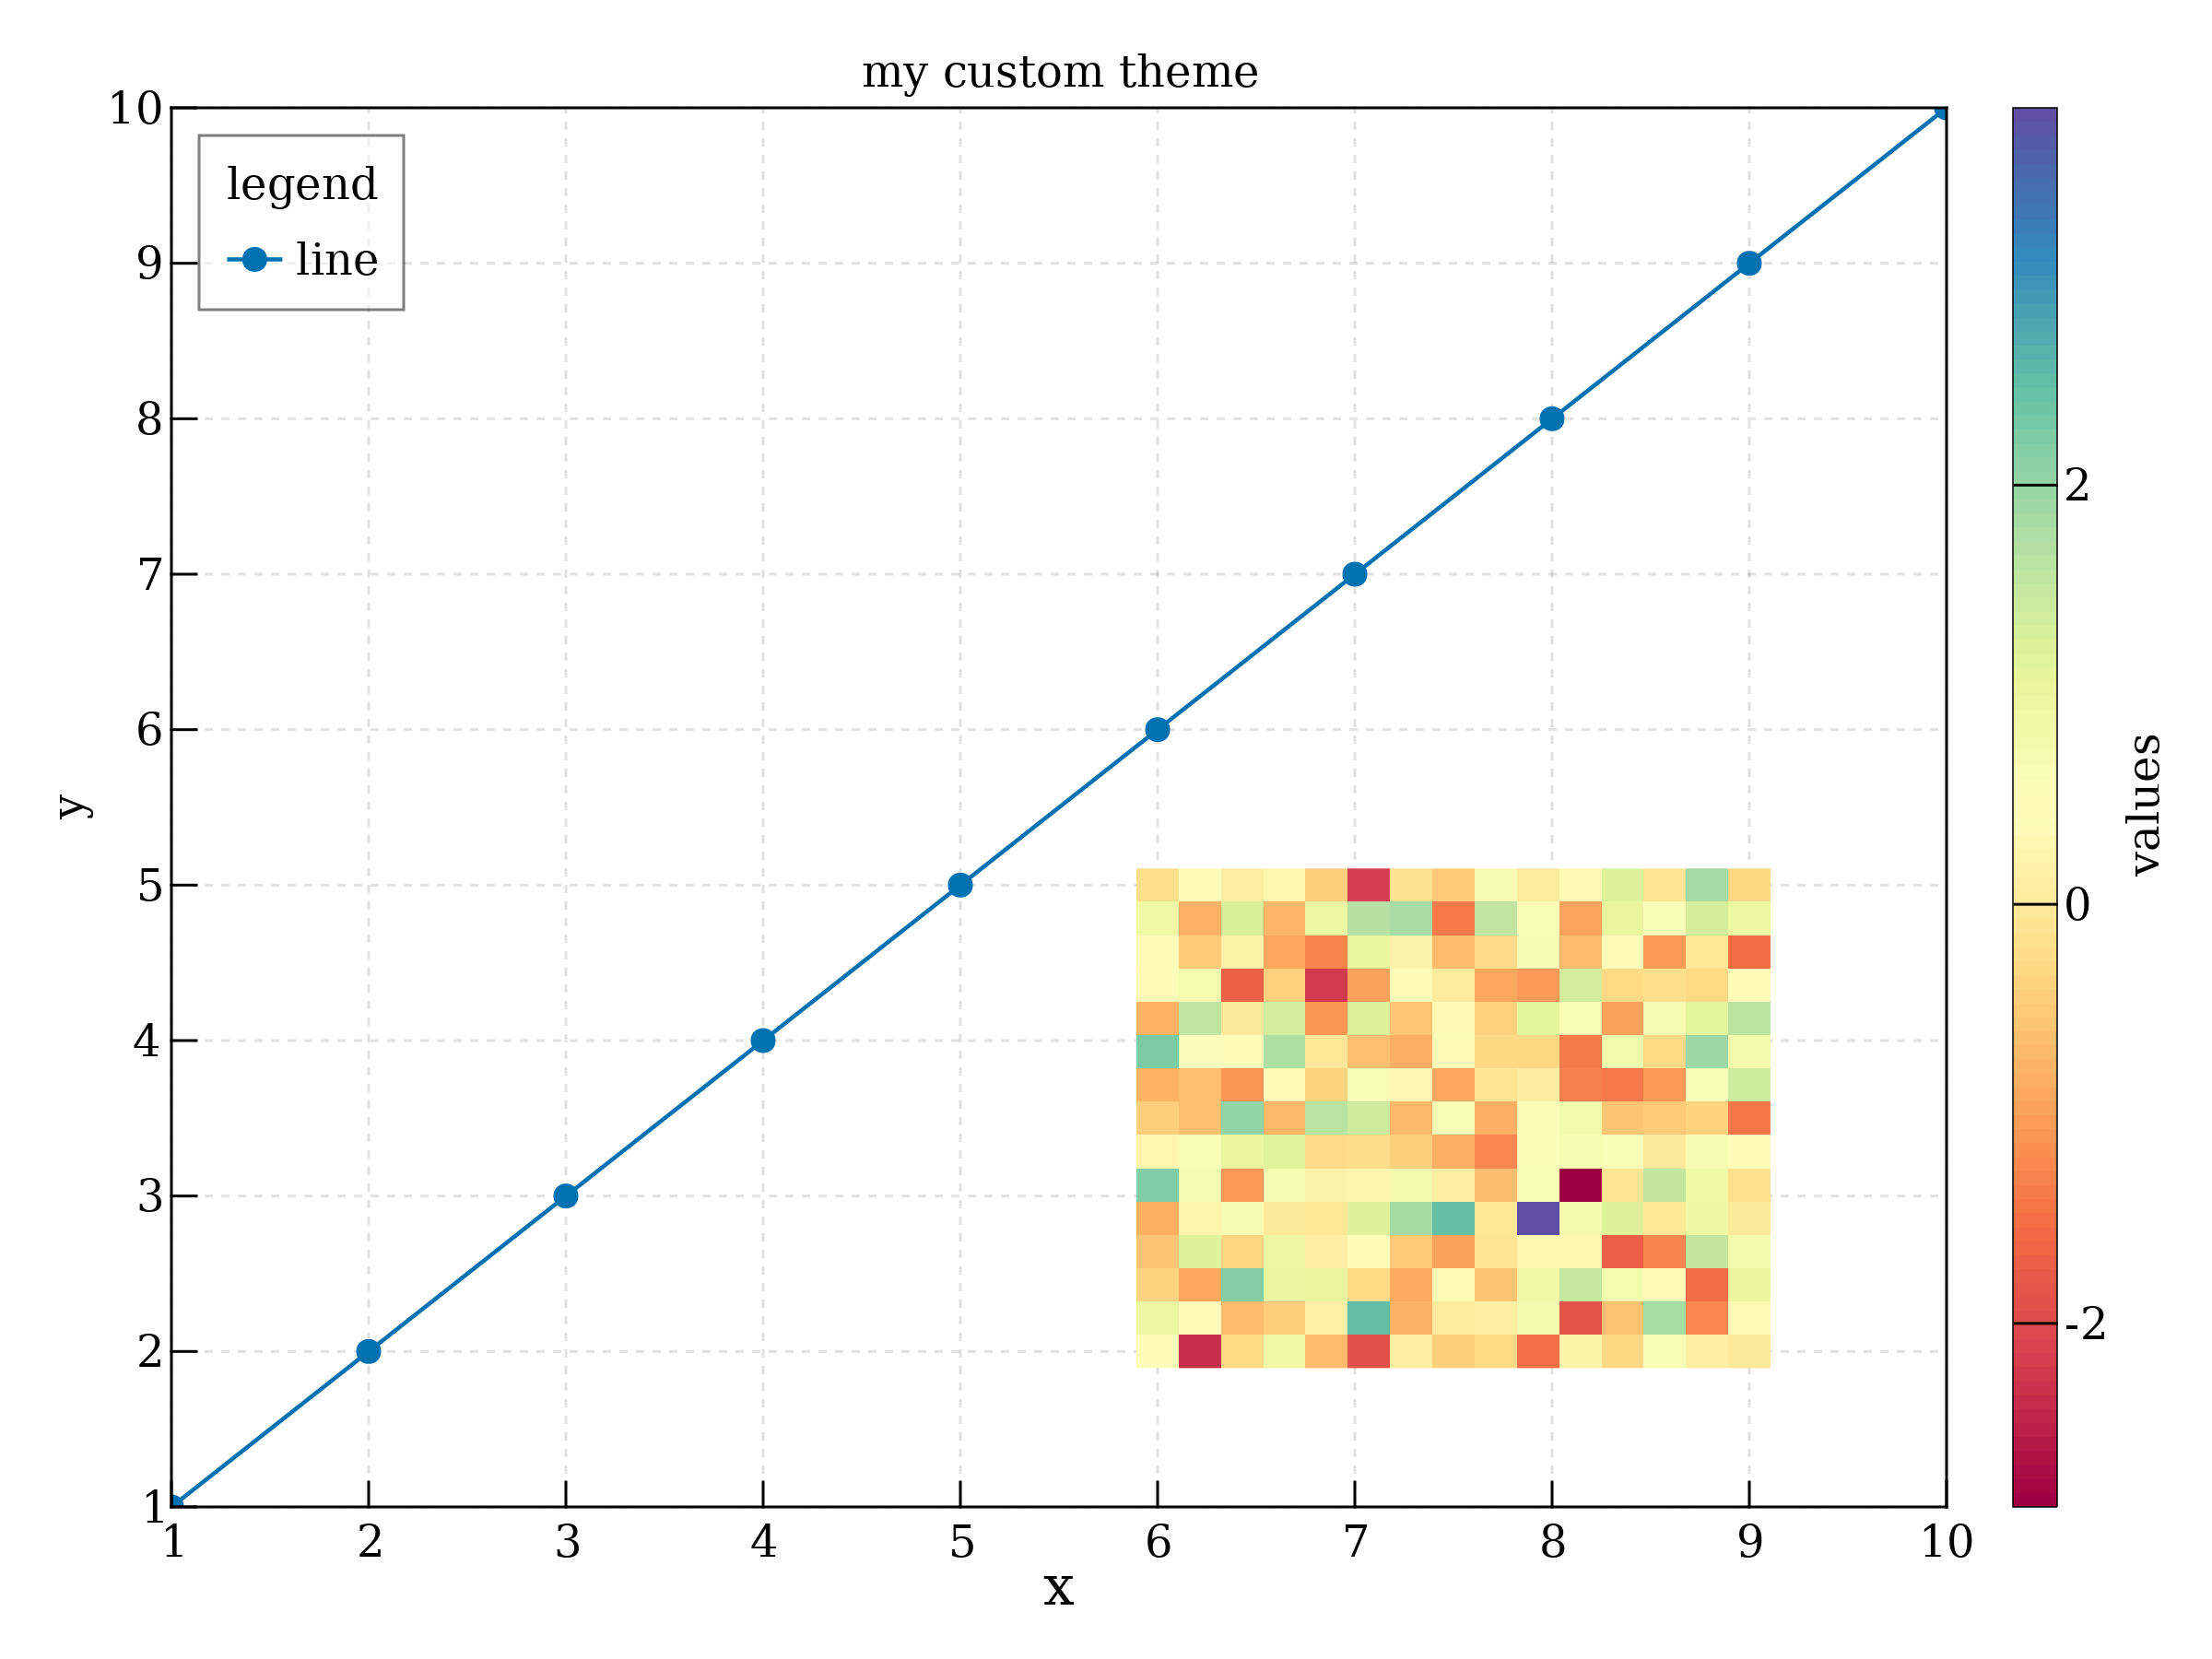
\includegraphics[width=0.6\textwidth,height=\textheight]{_build/im/plot_with_legend_and_colorbar.png}
\caption{Themed plot with Legend and
Colorbar.}\label{fig:plot_with_legend_and_colorbar}
}
\end{figure}

Agora, se algo precisar ser alterado após
\passthrough{\lstinline"set\_theme!(your\_theme)"}, podemos fazer isso
com
\passthrough{\lstinline"update\_theme!(resolution=(500, 400), fontsize=18)"},
por exemplo. Outra abordagem será passar argumentos adicionais para a
função \passthrough{\lstinline!with\_theme!}:

\begin{lstlisting}[language=Julia]
fig = (resolution=(600, 400), figure_padding=1, backgroundcolor=:grey90)
ax = (; aspect=DataAspect(), xlabel=L"x", ylabel=L"y")
cbar = (; height=Relative(4 / 5))
with_theme(publication_theme(); fig..., Axis=ax, Colorbar=cbar) do
    plot_with_legend_and_colorbar()
end
\end{lstlisting}

\begin{figure}
\hypertarget{fig:plot_theme_extra_args}{%
\centering
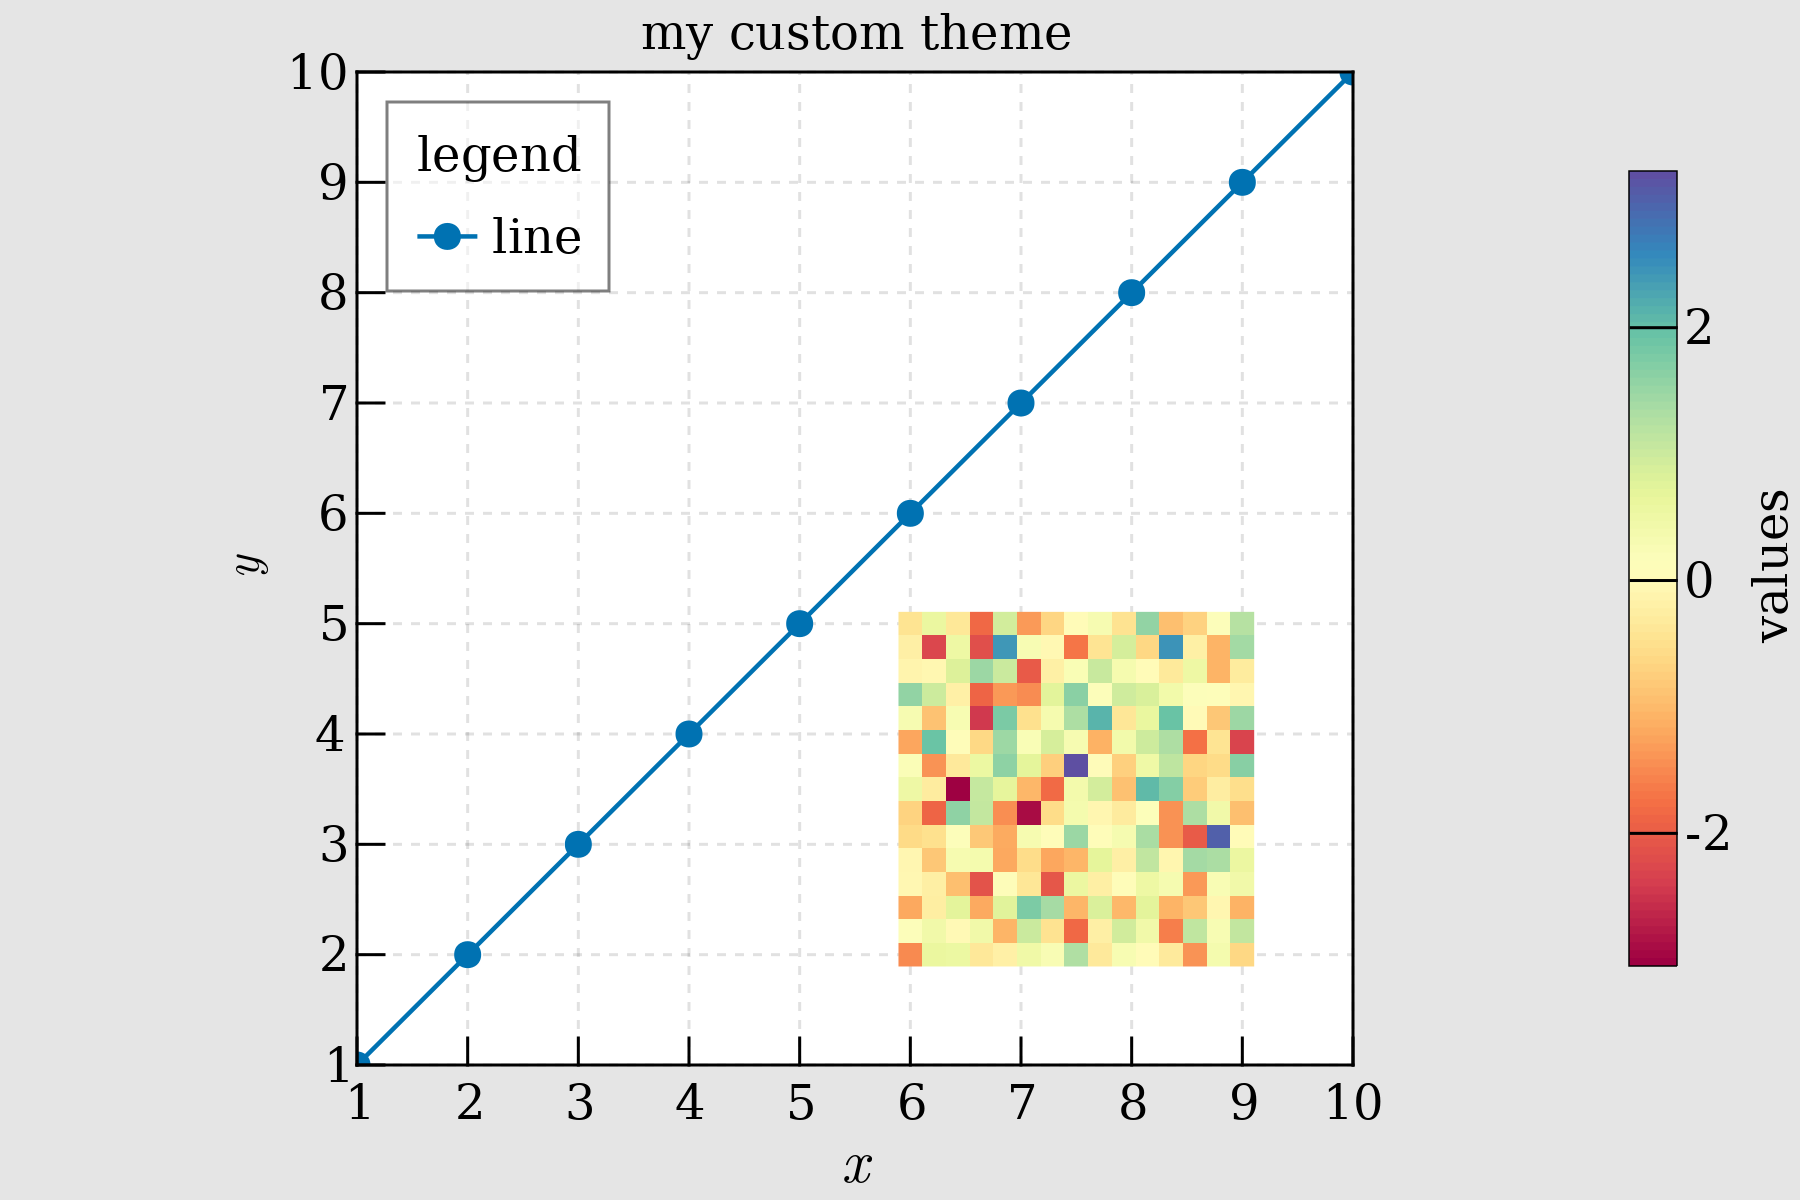
\includegraphics[width=0.6\textwidth,height=\textheight]{_build/im/plot_theme_extra_args.png}
\caption{Theme with extra args.}\label{fig:plot_theme_extra_args}
}
\end{figure}

Agora, vamos seguir em frente e fazer um \emph{plot} com strings em
LaTeX e um tema personalizado.

\hypertarget{usando-latexstrings.jl}{%
\section{Usando LaTeXStrings.jl}\label{usando-latexstrings.jl}}

Suporte LaTeX em \passthrough{\lstinline!Makie.jl!} também está
disponível via \passthrough{\lstinline!LaTeXStrings.jl!}:

\begin{lstlisting}
using LaTeXStrings
\end{lstlisting}

Casos de uso simples mostraremos abaixo
(Figure~\ref{fig:latex_strings}). Um exemplo básico inclui strings LaTeX
para rótulos e legendas x-y:

\begin{lstlisting}[language=Julia]
function LaTeX_Strings()
    x = 0:0.05:4π
    lines(x, x -> sin(3x) / (cos(x) + 2) / x; label=L"\frac{\sin(3x)}{x(\cos(x)+2)}",
        figure=(; resolution=(600, 400)), axis=(; xlabel=L"x"))
    lines!(x, x -> cos(x) / x; label=L"\cos(x)/x")
    lines!(x, x -> exp(-x); label=L"e^{-x}")
    limits!(-0.5, 13, -0.6, 1.05)
    axislegend(L"f(x)")
    current_figure()
end
\end{lstlisting}

\begin{lstlisting}[language=Julia]
with_theme(LaTeX_Strings, publication_theme())
\end{lstlisting}

\begin{figure}
\hypertarget{fig:latex_strings}{%
\centering
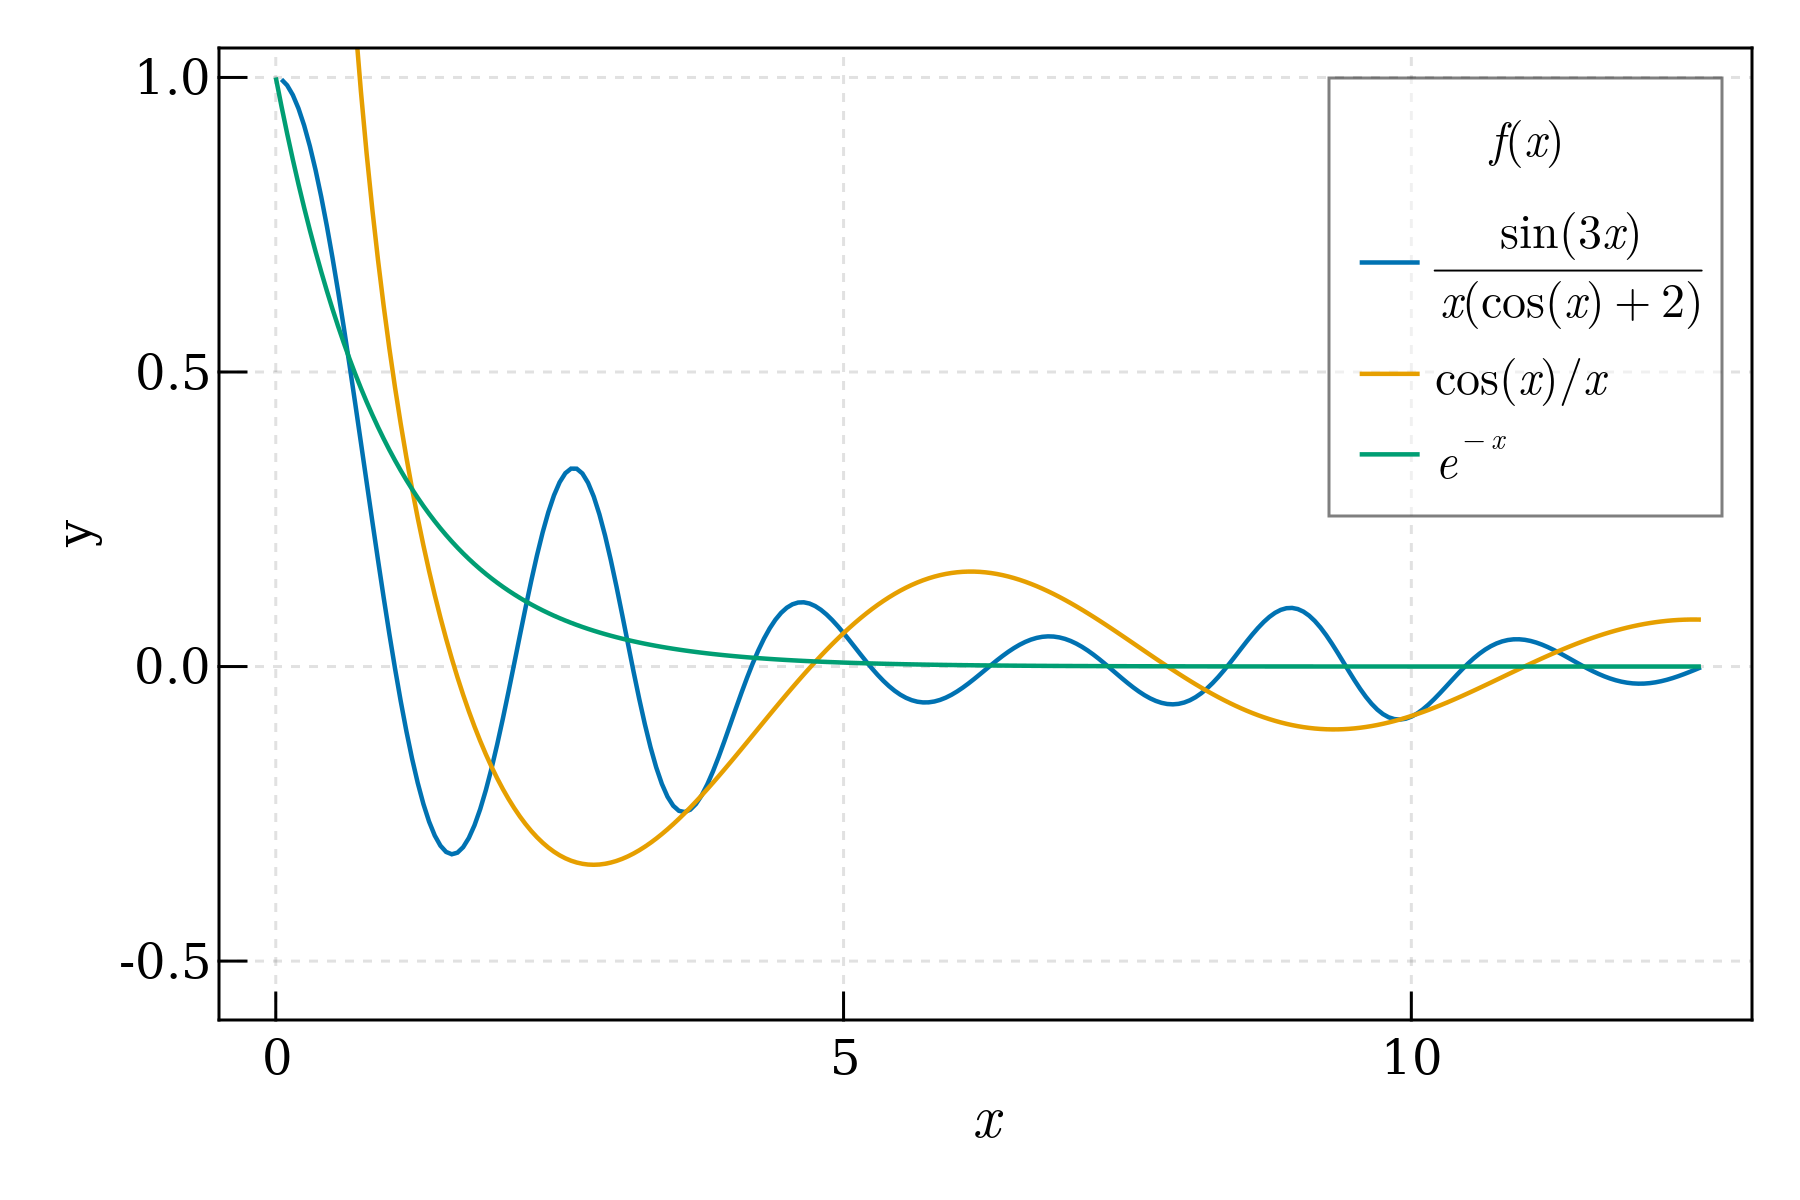
\includegraphics[width=0.6\textwidth,height=\textheight]{_build/im/latex_strings.png}
\caption{Plot with LaTeX strings.}\label{fig:latex_strings}
}
\end{figure}

Um exemplo mais complicado será com alguma equação como texto e
aumentando a numeração de legenda para curvas em um \emph{plot}:

\begin{lstlisting}[language=Julia]
function multiple_lines()
    x = collect(0:10)
    fig = Figure(resolution=(600, 400), font="CMU Serif")
    ax = Axis(fig[1, 1], xlabel=L"x", ylabel=L"f(x,a)")
    for i = 0:10
        lines!(ax, x, i .* x; label=latexstring("$(i) x"))
    end
    axislegend(L"f(x)"; position=:lt, nbanks=2, labelsize=14)
    text!(L"f(x,a) = ax", position=(4, 80))
    fig
end
multiple_lines()
\end{lstlisting}

\begin{figure}
\hypertarget{fig:multiple_lines}{%
\centering
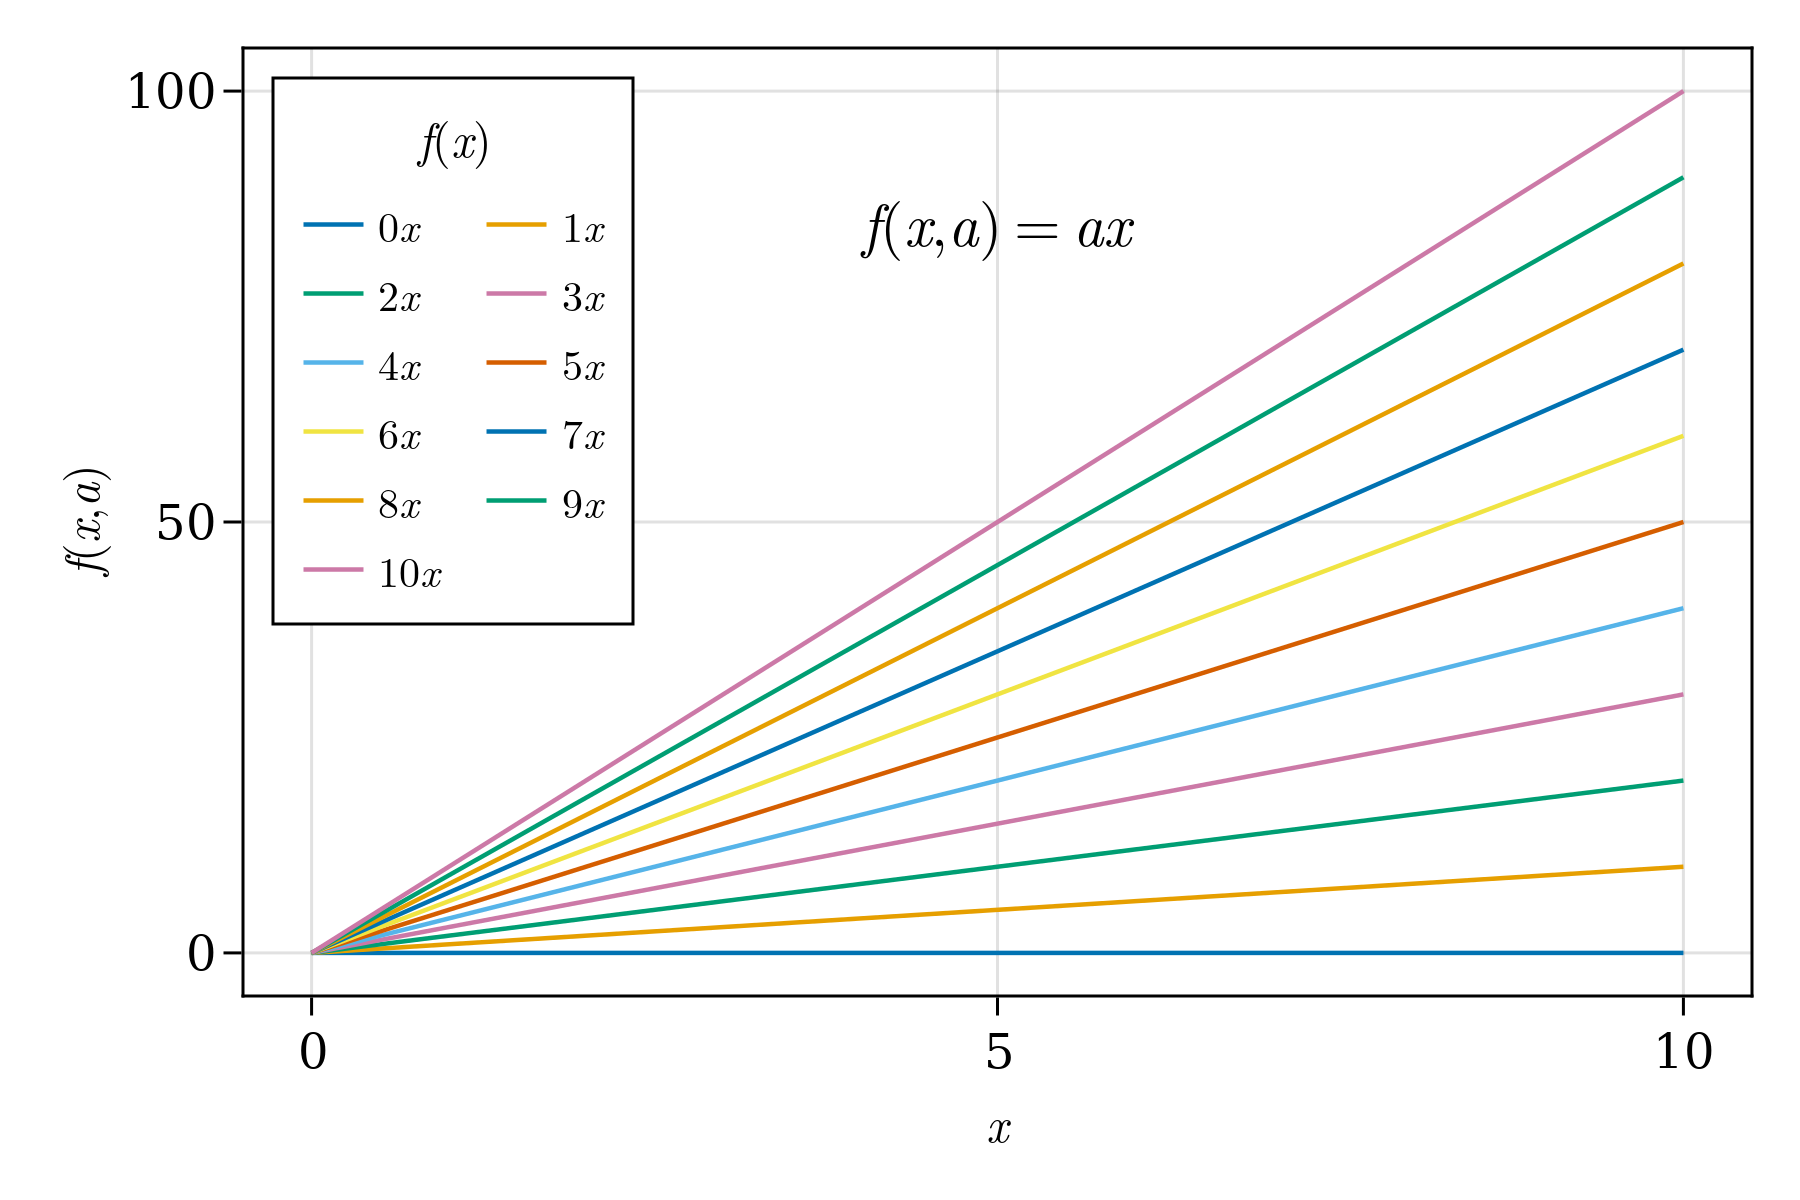
\includegraphics[width=0.6\textwidth,height=\textheight]{_build/im/JDS_multiple_lines_.png}
\caption{Multiple lines.}\label{fig:multiple_lines}
}
\end{figure}

Mas, algumas linhas têm cores repetidas, então isso não é bom. Adicionar
alguns marcadores e estilos de linha geralmente ajuda. Então, vamos
fazer isso usando
\href{http://makie.juliaplots.org/stable/documentation/theming/index.html\#cycles}{\passthrough{\lstinline!Cycles!}}
para esses tipos. Definir \passthrough{\lstinline!covary=true!} permite
alternar todos os elementos juntos:

\begin{lstlisting}[language=Julia]
function multiple_scatters_and_lines()
    x = collect(0:10)
    cycle = Cycle([:color, :linestyle, :marker], covary=true)
    set_theme!(Lines=(cycle=cycle,), Scatter=(cycle=cycle,))
    fig = Figure(resolution=(600, 400), font="CMU Serif")
    ax = Axis(fig[1, 1], xlabel=L"x", ylabel=L"f(x,a)")
    for i in x
        lines!(ax, x, i .* x; label=latexstring("$(i) x"))
        scatter!(ax, x, i .* x; markersize=13, strokewidth=0.25,
            label=latexstring("$(i) x"))
    end
    axislegend(L"f(x)"; merge=true, position=:lt, nbanks=2, labelsize=14)
    text!(L"f(x,a) = ax", position=(4, 80))
    set_theme!() # reset to default theme
    fig
end
multiple_scatters_and_lines()
\end{lstlisting}

\begin{figure}
\hypertarget{fig:multiple_scatters_and_lines}{%
\centering
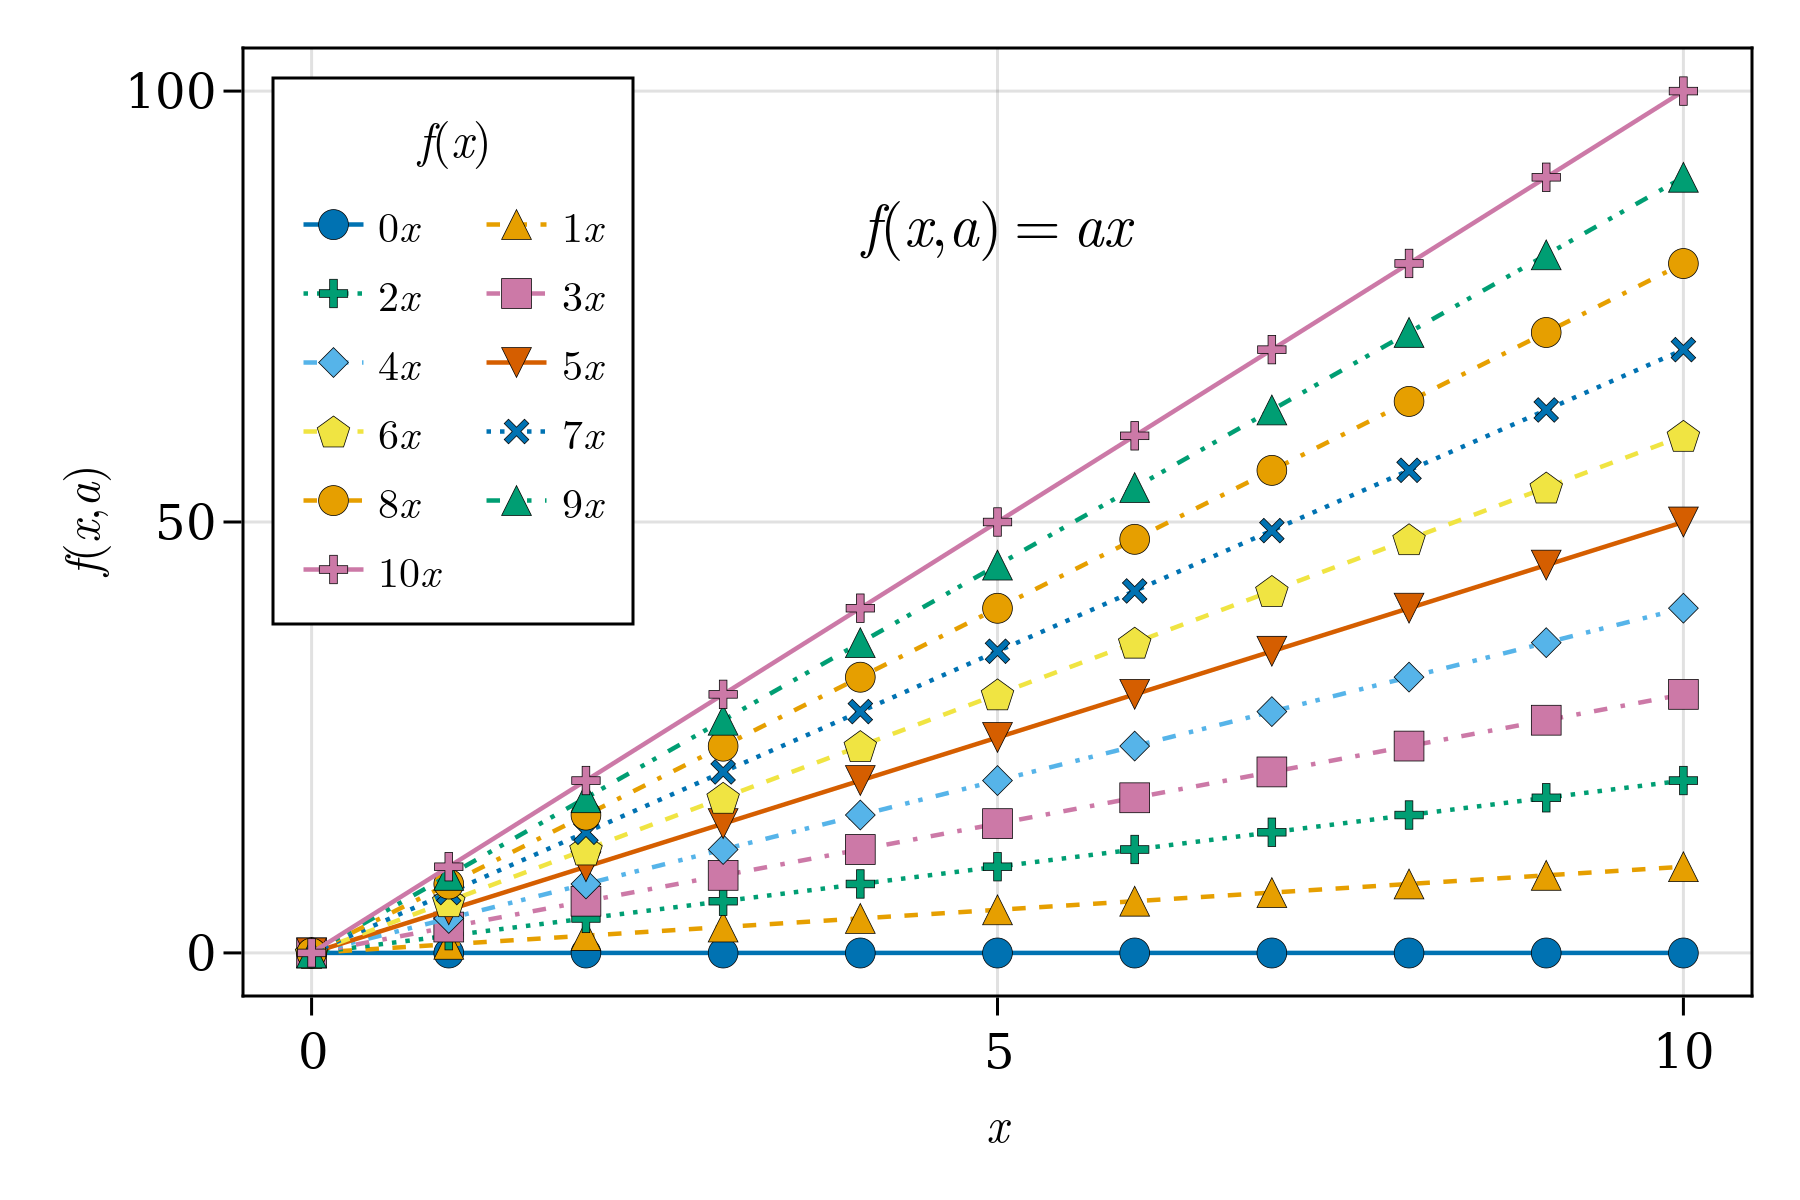
\includegraphics[width=0.6\textwidth,height=\textheight]{_build/im/JDS_multiple_scatters_and_lines_.png}
\caption{Multiple Scatters and
Lines.}\label{fig:multiple_scatters_and_lines}
}
\end{figure}

E voilà. Um \emph{plot} de qualidade de publicação está aqui. O que mais
podemos pedir? Bem, e quanto a diferentes cores ou paletas padrão? Em
nossa próxima seção, veremos como usar novamente
\href{http://makie.juliaplots.org/stable/documentation/theming/index.html\#cycles}{\passthrough{\lstinline!Cycles!}}
e conheça um pouco mais sobre eles, além de algumas palavras-chave
adicionais para conseguir isso.

\hypertarget{sec:makie_colors}{%
\section{Cores e mapas de cores}\label{sec:makie_colors}}

Escolher um conjunto apropriado de cores ou barra de cores para sua
plotagem é uma parte essencial para apresentação de resultados.
\href{https://github.com/JuliaGraphics/Colors.jl}{Colors.jl} é suportado
em \passthrough{\lstinline!Makie.jl!} para que você possa usar
\href{https://juliagraphics.github.io/Colors.jl/latest/namedcolors/}{cores
nomeadas} ou passar valores \passthrough{\lstinline!RGB!} ou
\passthrough{\lstinline!RGBA!}. Além disso, os mapas de cores
\href{https://github.com/JuliaGraphics/ColorSchemes.jl}{ColorSchemes.jl}
e
\href{https://github.com/peterkovesi/PerceptualColourMaps.jl}{PerceptualColourMaps.jl}
também podem ser usados. Vale a pena saber que você pode reverter um
mapa de cores fazendo \passthrough{\lstinline!Reverse(:colormap\_name)!}
para obter uma cor transparente ou mapa de cores com
\passthrough{\lstinline!color=(:red,0.5)!} e
\passthrough{\lstinline!colormap=(:viridis, 0.5)!}.

Diferentes casos de uso serão mostrados a seguir. Então vamos definir um
tema personalizado com novas cores e uma paleta de cores.

Por padrão \passthrough{\lstinline!Makie.jl!} tem um conjunto
predefinido de cores para percorrê-las automaticamente. Conforme
mostrado nas figuras anteriores, onde nenhuma cor específica foi
definida. A substituição desses padrões é feita chamando a palavra-chave
\passthrough{\lstinline!color!} na função de plotagem e especificando
uma nova cor por meio de um \passthrough{\lstinline!Symbol!} ou
\passthrough{\lstinline!String!}. Veja isso em ação no exemplo a seguir:

\begin{lstlisting}[language=Julia]
function set_colors_and_cycle()
    # Epicycloid lines
    x(r, k, θ) = r * (k .+ 1.0) .* cos.(θ) .- r * cos.((k .+ 1.0) .* θ)
    y(r, k, θ) = r * (k .+ 1.0) .* sin.(θ) .- r * sin.((k .+ 1.0) .* θ)
    θ = LinRange(0, 6.2π, 1000)
    axis = (; xlabel=L"x(\theta)", ylabel=L"y(\theta)",
        title="Epicycloid", aspect=DataAspect())
    figure = (; resolution=(600, 400), font="CMU Serif")
    fig, ax, _ = lines(x(1, 1, θ), y(1, 1, θ); color="firebrick1", # string
        label=L"1.0", axis=axis, figure=figure)
    lines!(ax, x(4, 2, θ), y(4, 2, θ); color=:royalblue1, #symbol
        label=L"2.0")
    for k = 2.5:0.5:5.5
        lines!(ax, x(2k, k, θ), y(2k, k, θ); label=latexstring("$(k)")) #cycle
    end
    Legend(fig[1, 2], ax, latexstring("k, r = 2k"), merge=true)
    fig
end
set_colors_and_cycle()
\end{lstlisting}

\begin{figure}
\hypertarget{fig:set_colors_and_cycle}{%
\centering
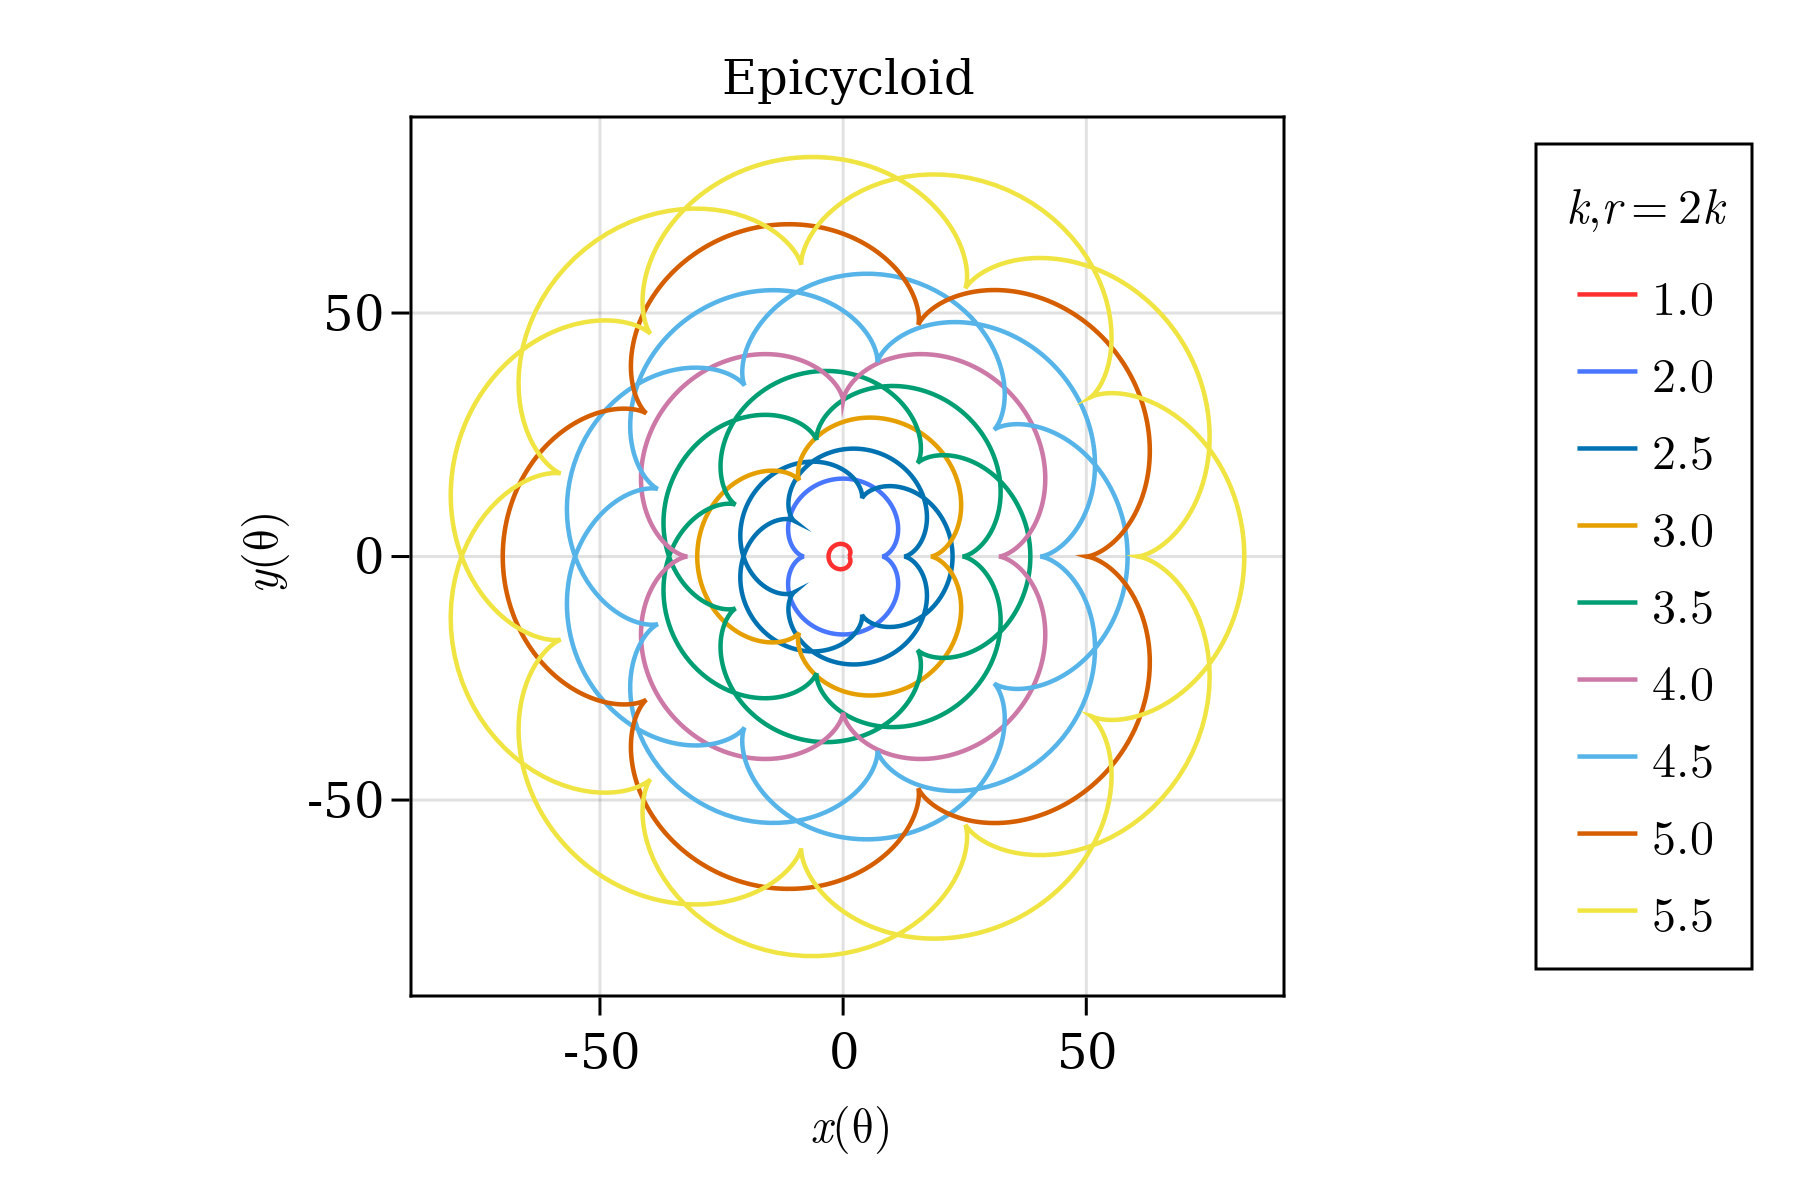
\includegraphics{_build/im/JDS_set_colors_and_cycle_.png}
\caption{Set colors and cycle.}\label{fig:set_colors_and_cycle}
}
\end{figure}

Onde, nas duas primeiras linhas, usamos a palavra-chave
\passthrough{\lstinline!color!} para especificar nossa cor. O resto está
usando o padrão do conjunto de cores do ciclo. Mais tarde, aprenderemos
como fazer um ciclo personalizado.

Em relação aos mapas de cores, já estamos familiarizados com a
palavra-chave \passthrough{\lstinline!colormap!} para
\passthrough{\lstinline!heatmap!}s e \passthrough{\lstinline!scatter!}s.
Aqui, mostramos que um mapa de cores também pode ser especificado por
meio de um \passthrough{\lstinline!Symbol!} ou uma
\passthrough{\lstinline!String!}, semelhante a cores. Ou até mesmo um
vetor de cores \passthrough{\lstinline!RGB!}. Vamos fazer nosso primeiro
exemplo chamando mapas de cores como \passthrough{\lstinline!Symbol!},
\passthrough{\lstinline!String!} e \passthrough{\lstinline!cgrad!} para
valores categóricos. Cheque \passthrough{\lstinline!?cgrad!} para mais
informações.

\begin{lstlisting}[language=Julia]
figure = (; resolution=(600, 400), font="CMU Serif")
axis = (; xlabel=L"x", ylabel=L"y", aspect=DataAspect())
fig, ax, pltobj = heatmap(rand(20, 20); colorrange=(0, 1),
    colormap=Reverse(:viridis), axis=axis, figure=figure)
Colorbar(fig[1, 2], pltobj, label = "Reverse colormap Sequential")
fig
\end{lstlisting}

\begin{figure}
\hypertarget{fig:Reverse_colormap_sequential}{%
\centering
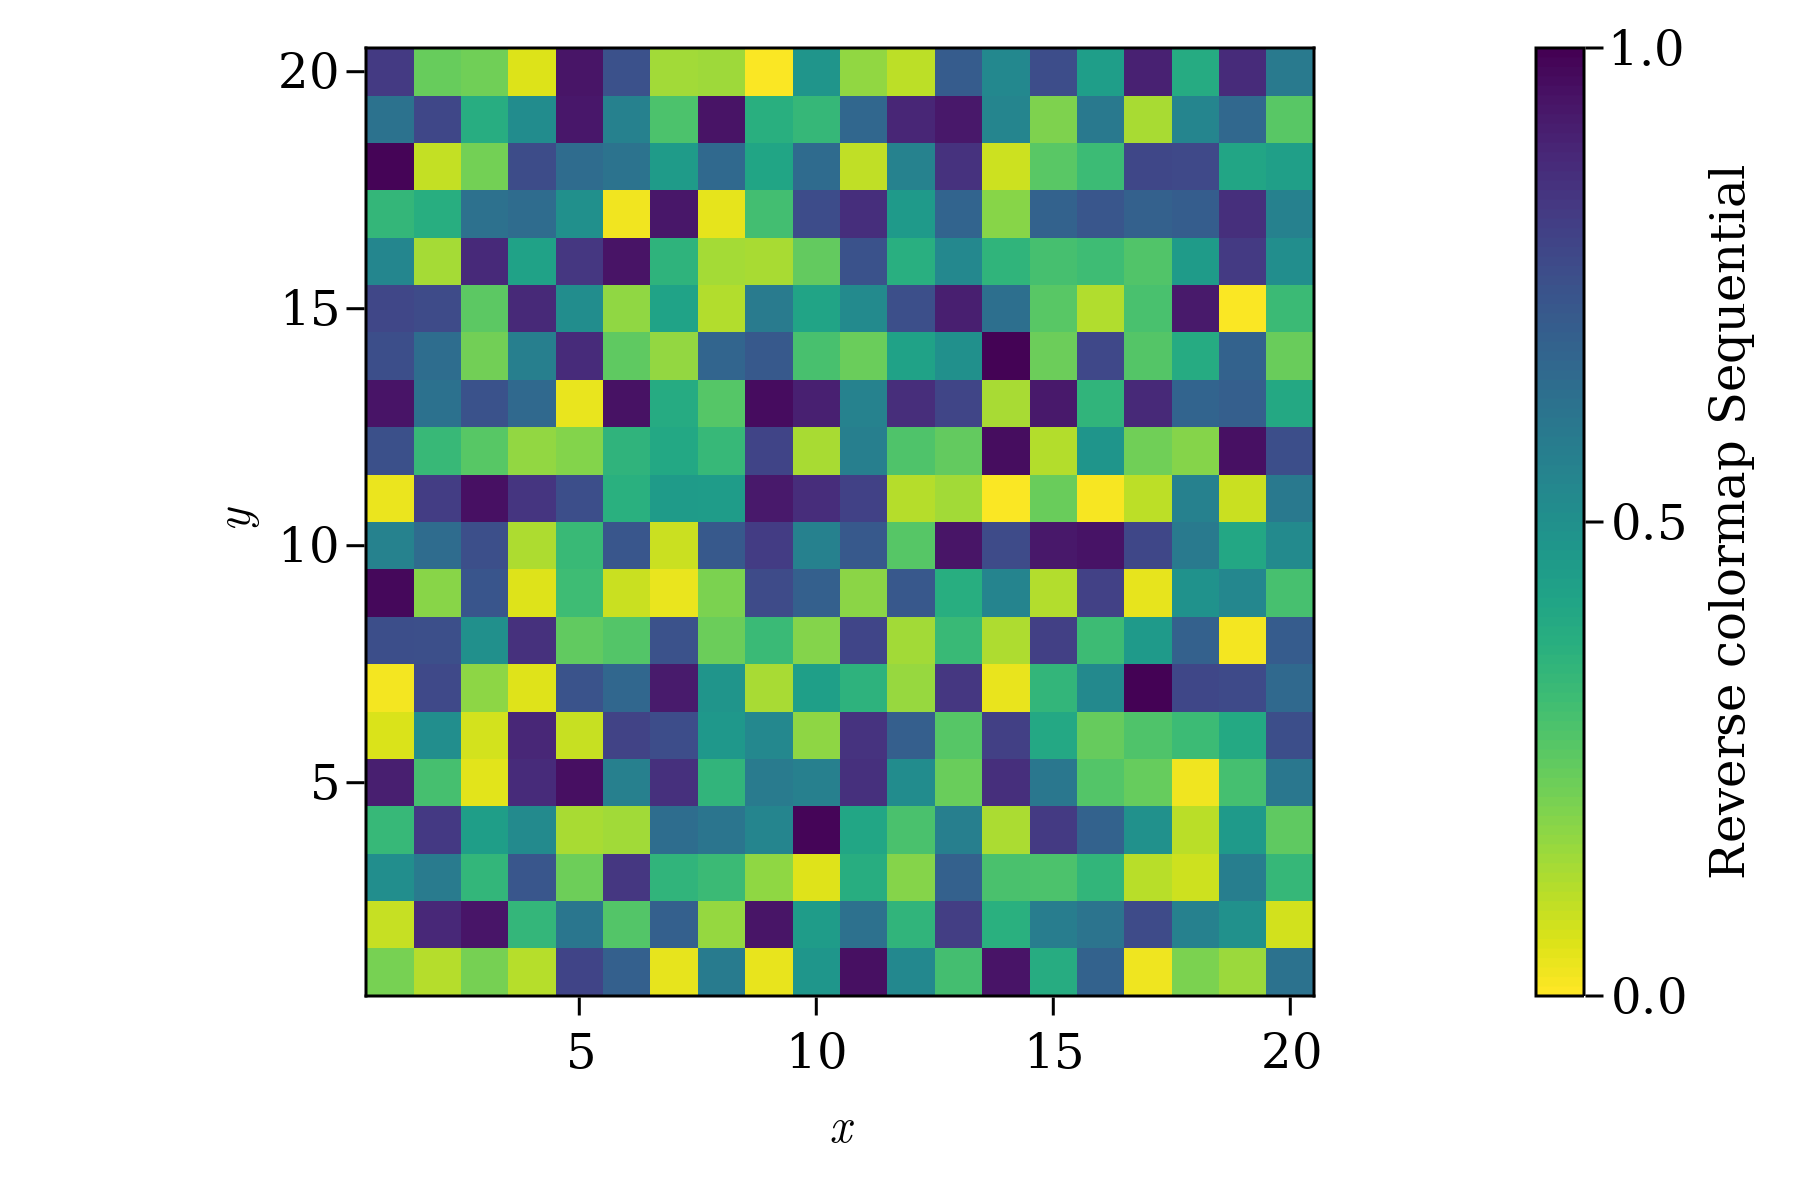
\includegraphics[width=0.6\textwidth,height=\textheight]{_build/im/Reverse_colormap_sequential.png}
\caption{Reverse colormap sequential and
colorrange.}\label{fig:Reverse_colormap_sequential}
}
\end{figure}

Ao definir um \passthrough{\lstinline!colorrange!} geralmente os valores
fora deste intervalo são coloridos com a primeira e a última cor do mapa
de cores. No entanto, às vezes é melhor especificar a cor desejada em
ambas as extremidades. Fazemos isso com
\passthrough{\lstinline!highclip!} e \passthrough{\lstinline!lowclip!}:

\begin{lstlisting}
using ColorSchemes
\end{lstlisting}

\begin{lstlisting}[language=Julia]
figure = (; resolution=(600, 400), font="CMU Serif")
axis = (; xlabel=L"x", ylabel=L"y", aspect=DataAspect())
fig, ax, pltobj=heatmap(randn(20, 20); colorrange=(-2, 2),
    colormap="diverging_rainbow_bgymr_45_85_c67_n256",
    highclip=:black, lowclip=:white, axis=axis, figure=figure)
Colorbar(fig[1, 2], pltobj, label = "Diverging colormap")
fig
\end{lstlisting}

\begin{figure}
\hypertarget{fig:diverging_colormap}{%
\centering
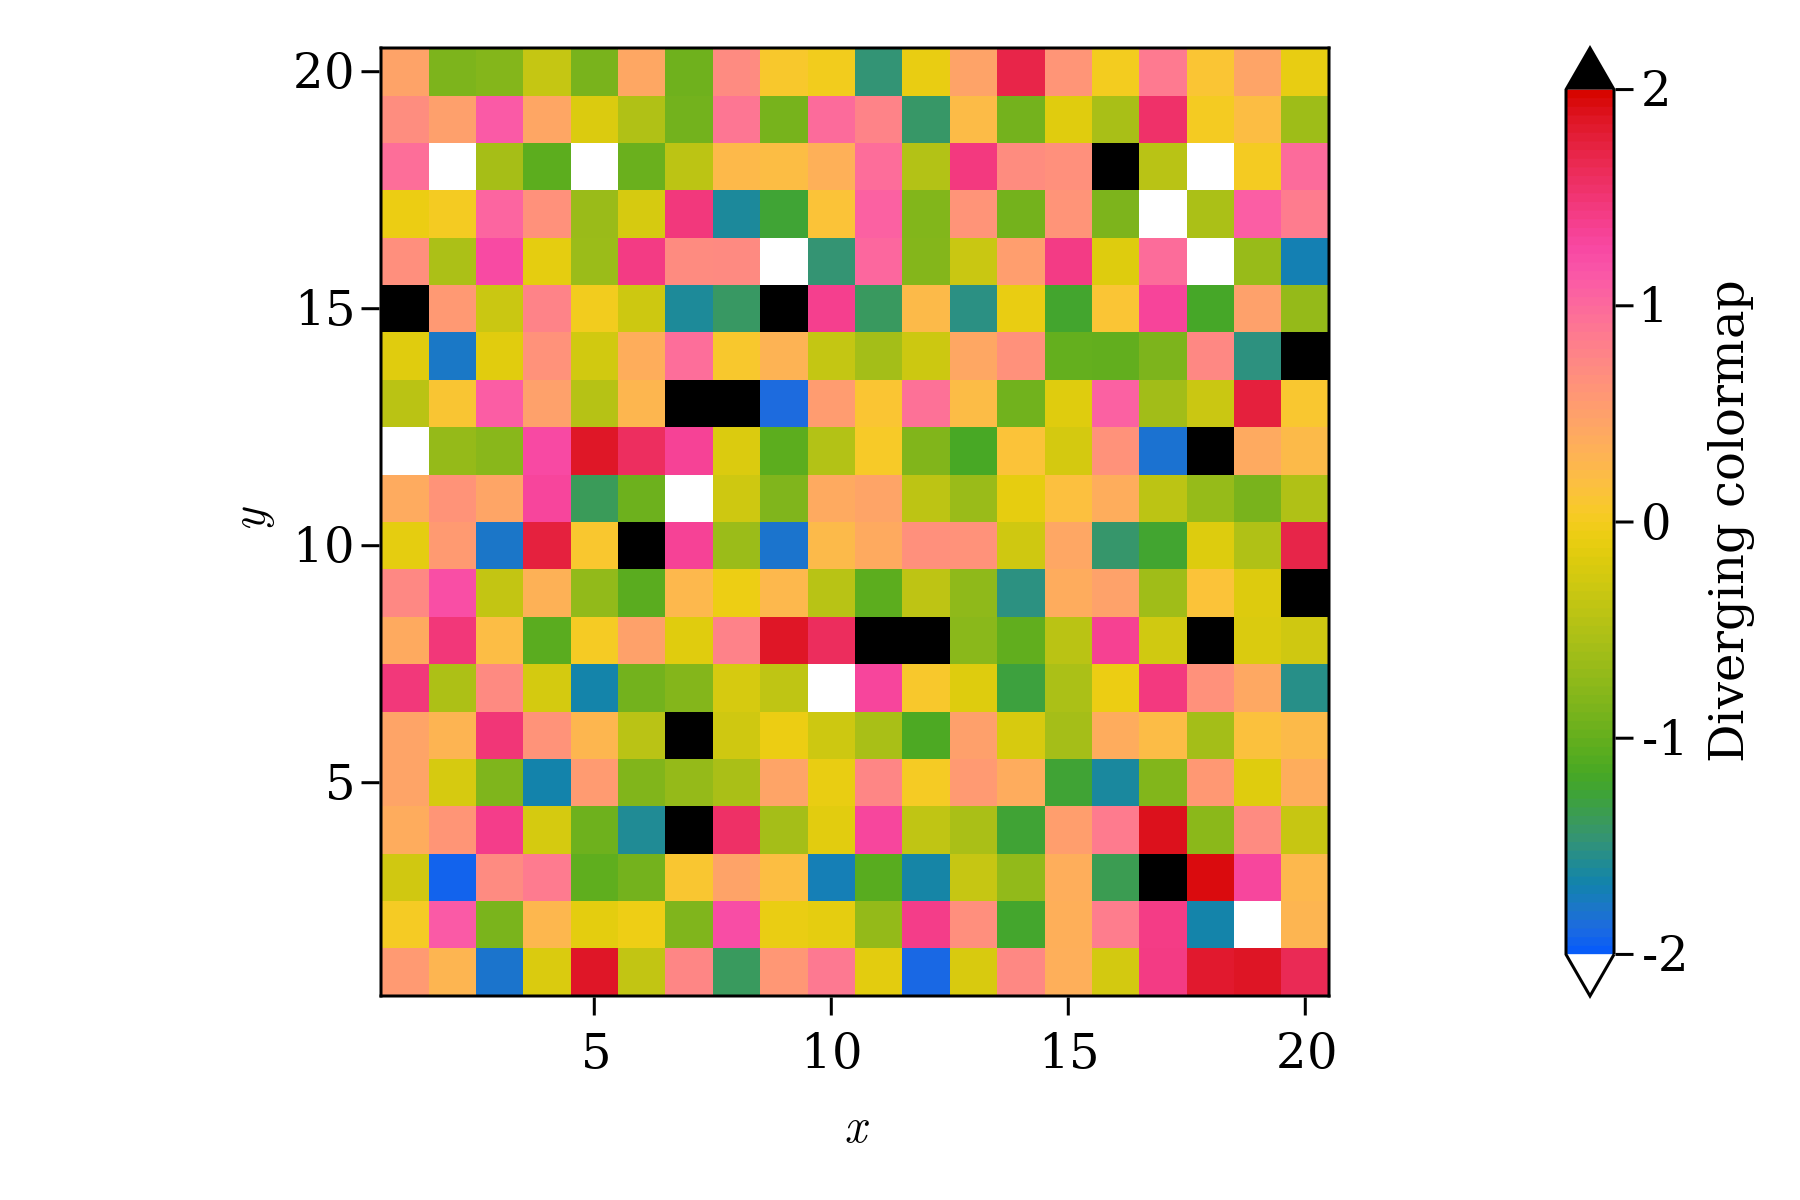
\includegraphics[width=0.6\textwidth,height=\textheight]{_build/im/diverging_colormap.png}
\caption{Diverging Colormap with low and high
clip.}\label{fig:diverging_colormap}
}
\end{figure}

Mas mencionamos que também vetores \passthrough{\lstinline!RGB!} são
opções válidas. Para o nosso próximo exemplo, você pode passar o mapa de
cores personalizado \emph{perse} ou usar \passthrough{\lstinline!cgrad!}
para forçar um \passthrough{\lstinline!Colorbar!} categórico.

\begin{lstlisting}
using Colors, ColorSchemes
\end{lstlisting}

\begin{lstlisting}[language=Julia]
figure = (; resolution=(600, 400), font="CMU Serif")
axis = (; xlabel=L"x", ylabel=L"y", aspect=DataAspect())
cmap = ColorScheme(range(colorant"red", colorant"green", length=3))
mygrays = ColorScheme([RGB{Float64}(i, i, i) for i in [0.0, 0.5, 1.0]])
fig, ax, pltobj = heatmap(rand(-1:1, 20, 20);
    colormap=cgrad(mygrays, 3, categorical=true, rev=true), # cgrad and Symbol, mygrays,
    axis=axis, figure=figure)
cbar = Colorbar(fig[1, 2], pltobj, label="Categories")
cbar.ticks = ([-0.66, 0, 0.66], ["-1", "0", "1"])
fig
\end{lstlisting}

\begin{figure}
\hypertarget{fig:categorical_colormap}{%
\centering
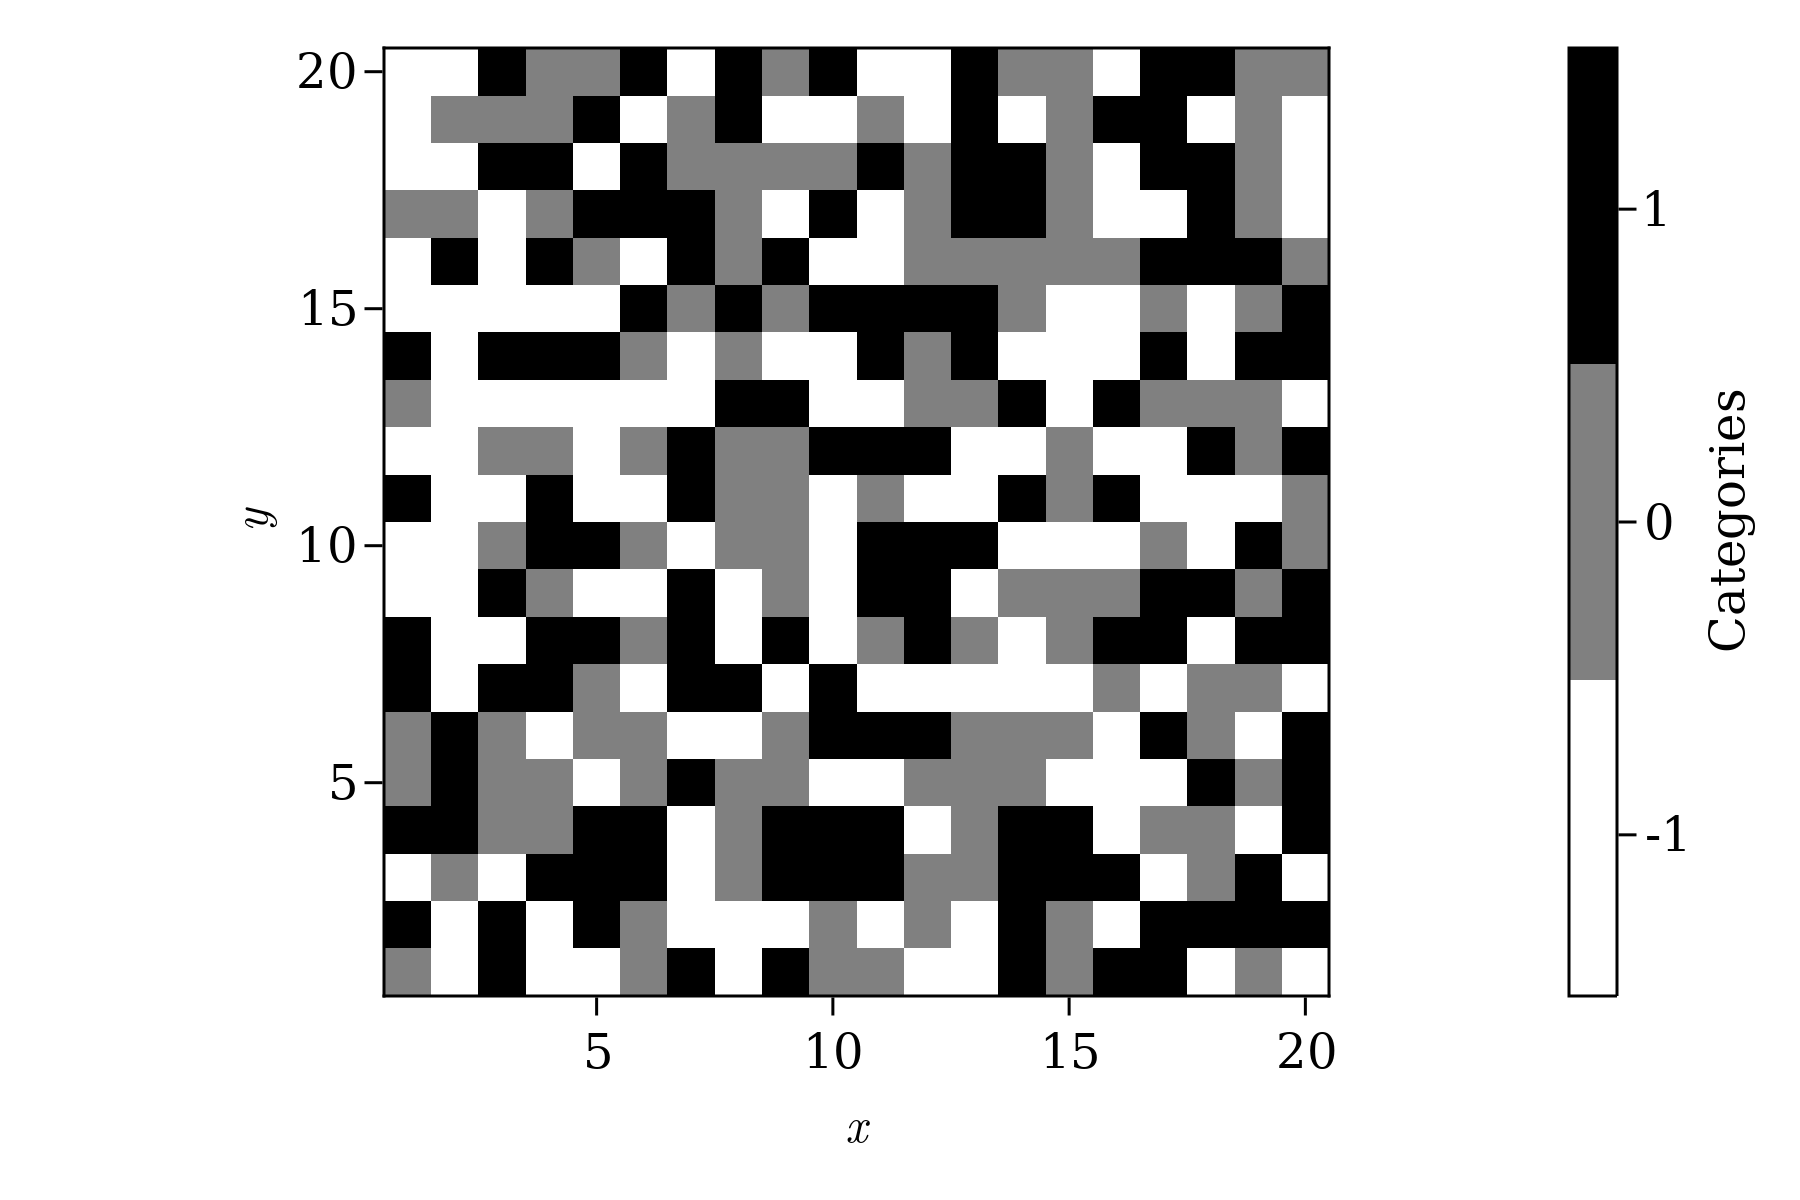
\includegraphics[width=0.6\textwidth,height=\textheight]{_build/im/categorical_colormap.png}
\caption{Categorical Colormap.}\label{fig:categorical_colormap}
}
\end{figure}

Por fim, os tiques na barra de cores para o caso categorial não são
centralizados por padrão em cada cor. Isso é corrigido passando ticks
personalizados, como em
\passthrough{\lstinline!cbar.ticks = (positions, ticks)!}. A última
situação é passar uma tupla de duas cores para o
\passthrough{\lstinline!colormap!} como símbolos, strings ou uma
mistura. Você obterá um mapa de cores interpolado entre essas duas
cores.

Além disso, cores codificadas em hexadecimal também são aceitas. Então,
no topo do nosso mapa de calor, vamos colocar um ponto semitransparente
usando:

\begin{lstlisting}[language=Julia]
figure = (; resolution=(600, 400), font="CMU Serif")
axis = (; xlabel=L"x", ylabel=L"y", aspect=DataAspect())
fig, ax, pltobj = heatmap(rand(20, 20); colorrange=(0, 1),
    colormap=(:red, "black"), axis=axis, figure=figure)
scatter!(ax, [11], [11], color=("#C0C0C0", 0.5), markersize=150)
Colorbar(fig[1, 2], pltobj, label="2 colors")
fig
\end{lstlisting}

\begin{figure}
\hypertarget{fig:colormap_two_colors}{%
\centering
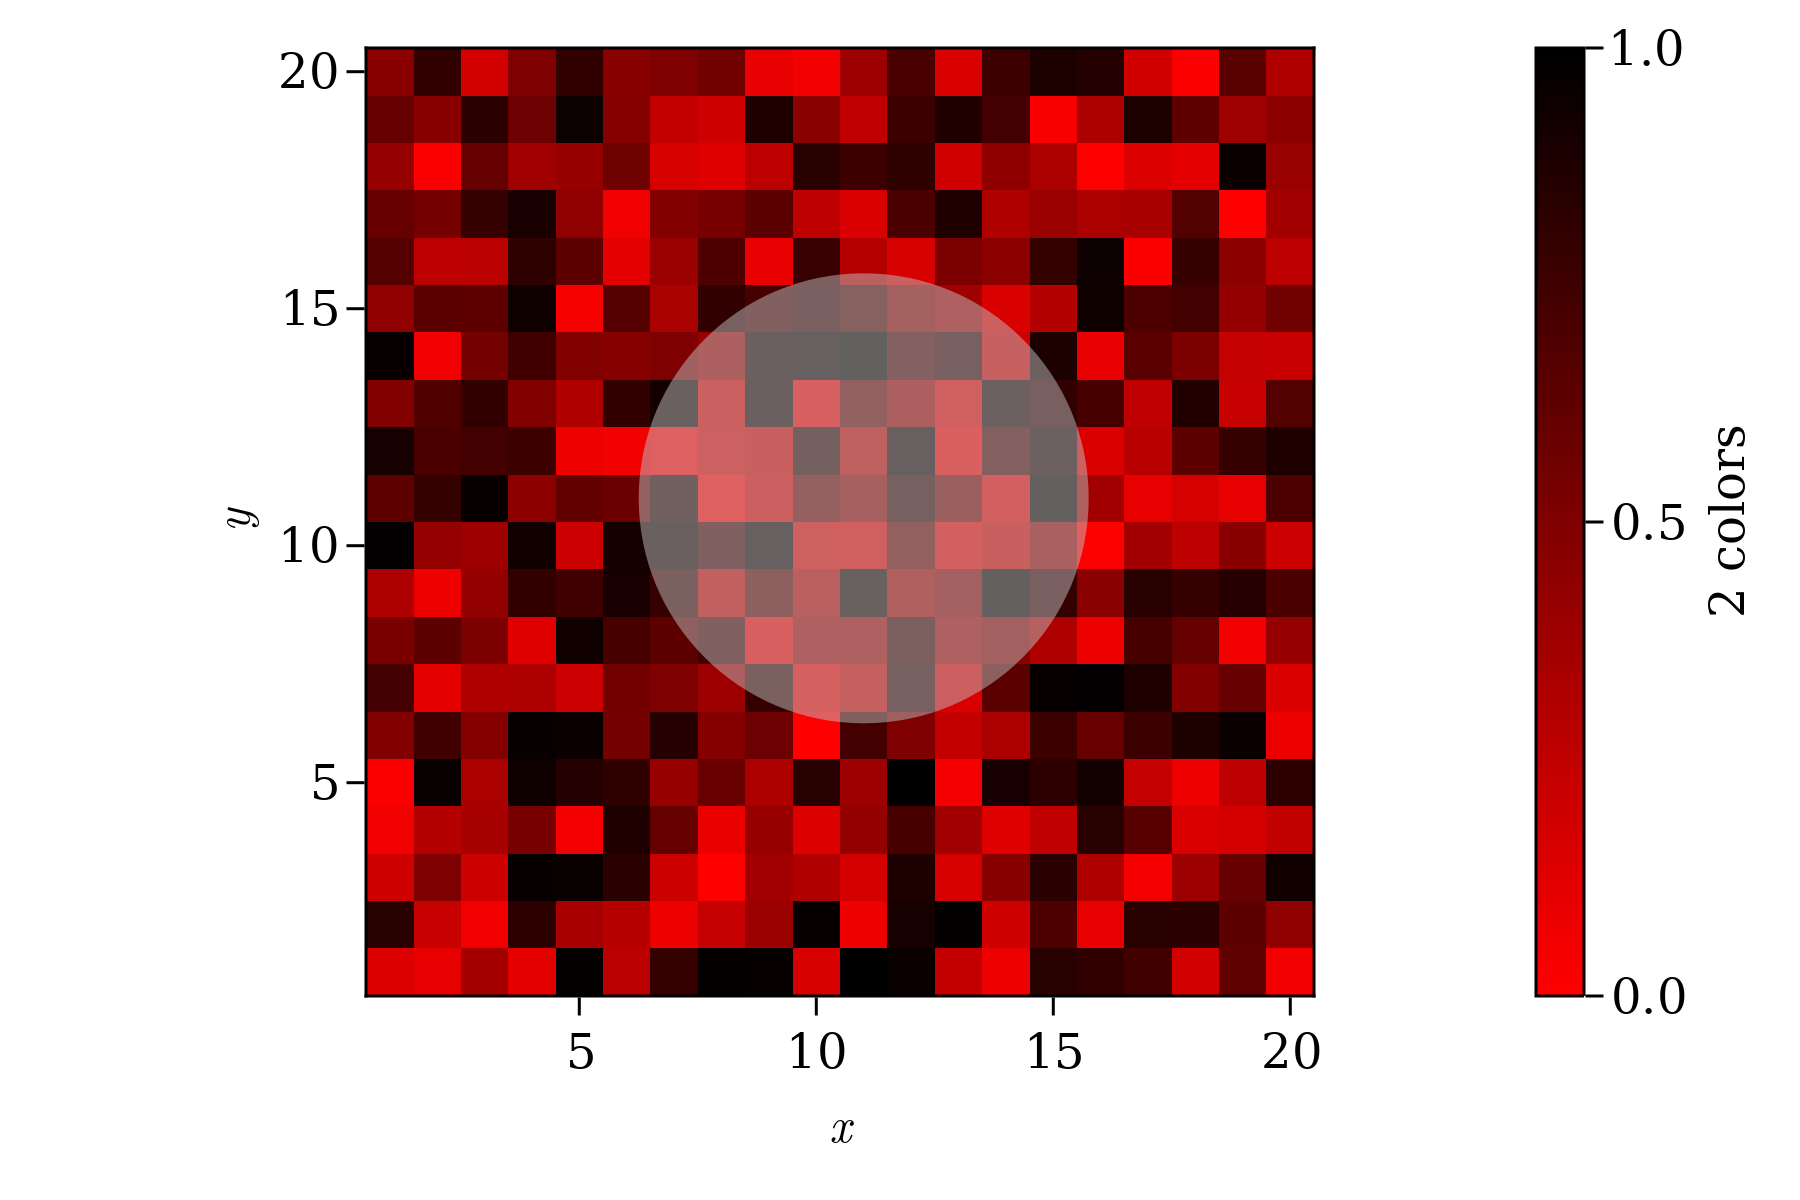
\includegraphics[width=0.6\textwidth,height=\textheight]{_build/im/colormap_two_colors.png}
\caption{Colormap from two colors.}\label{fig:colormap_two_colors}
}
\end{figure}

\hypertarget{ciclo-personalizado}{%
\subsection{Ciclo personalizado}\label{ciclo-personalizado}}

Aqui, poderíamos definir um \passthrough{\lstinline!Tema!} global com um
novo ciclo de cores, mas essa \textbf{não é a maneira recomendada} de
fazer isso. É melhor definir um novo tema e usar como mostramos antes.
Vamos definir um novo com um \passthrough{\lstinline!cycle!} para
\passthrough{\lstinline!:color!}, \passthrough{\lstinline!:linestyle!},
\passthrough{\lstinline!:marker!} e um novo padrão
\passthrough{\lstinline!colormap!}. Vamos adicionar esses novos
atributos ao nosso \passthrough{\lstinline!publication\_theme!}
anterior.

\begin{lstlisting}[language=Julia]
function new_cycle_theme()
    # https://nanx.me/ggsci/reference/pal_locuszoom.html
    my_colors = ["#D43F3AFF", "#EEA236FF", "#5CB85CFF", "#46B8DAFF",
        "#357EBDFF", "#9632B8FF", "#B8B8B8FF"]
    cycle = Cycle([:color, :linestyle, :marker], covary=true) # alltogether
    my_markers = [:circle, :rect, :utriangle, :dtriangle, :diamond,
        :pentagon, :cross, :xcross]
    my_linestyle = [nothing, :dash, :dot, :dashdot, :dashdotdot]
    Theme(
        fontsize=16, font="CMU Serif",
        colormap=:linear_bmy_10_95_c78_n256,
        palette=(color=my_colors, marker=my_markers, linestyle=my_linestyle),
        Lines=(cycle=cycle,), Scatter=(cycle=cycle,),
        Axis=(xlabelsize=20, xgridstyle=:dash, ygridstyle=:dash,
            xtickalign=1, ytickalign=1, yticksize=10, xticksize=10,
            xlabelpadding=-5, xlabel="x", ylabel="y"),
        Legend=(framecolor=(:black, 0.5), bgcolor=(:white, 0.5)),
        Colorbar=(ticksize=16, tickalign=1, spinewidth=0.5),
    )
end
\end{lstlisting}

E aplique-o a uma função de plotagem como a seguinte:

\begin{lstlisting}[language=Julia]
function scatters_and_lines()
    x = collect(0:10)
    xh = LinRange(4, 6, 25)
    yh = LinRange(70, 95, 25)
    h = randn(25, 25)
    fig = Figure(resolution=(600, 400), font="CMU Serif")
    ax = Axis(fig[1, 1], xlabel=L"x", ylabel=L"f(x,a)")
    for i in x
        lines!(ax, x, i .* x; label=latexstring("$(i) x"))
        scatter!(ax, x, i .* x; markersize=13, strokewidth=0.25,
            label=latexstring("$(i) x"))
    end
    hm = heatmap!(xh, yh, h)
    axislegend(L"f(x)"; merge=true, position=:lt, nbanks=2, labelsize=14)
    Colorbar(fig[1, 2], hm, label="new default colormap")
    limits!(ax, -0.5, 10.5, -5, 105)
    colgap!(fig.layout, 5)
    fig
end
\end{lstlisting}

\begin{lstlisting}[language=Julia]
with_theme(scatters_and_lines, new_cycle_theme())
\end{lstlisting}

\begin{figure}
\hypertarget{fig:custom_cycle}{%
\centering
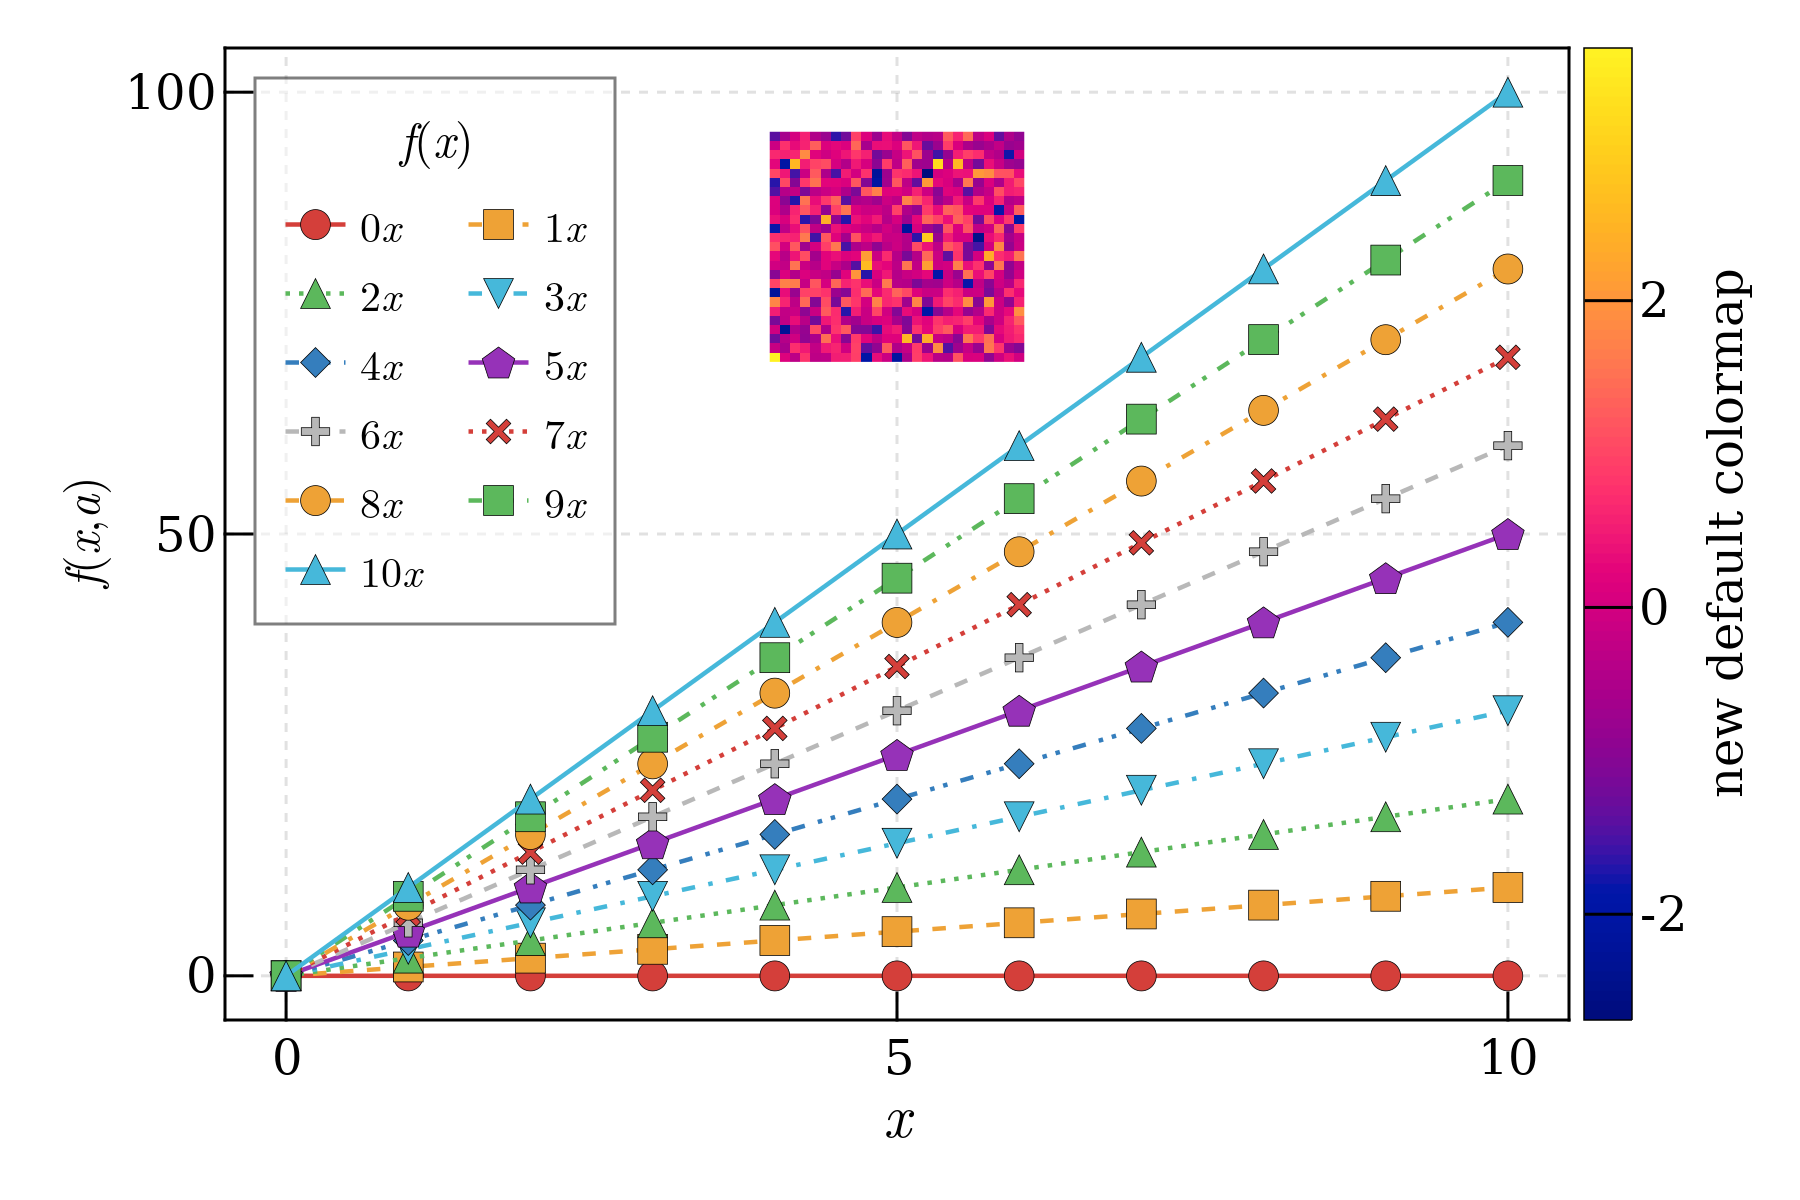
\includegraphics[width=0.6\textwidth,height=\textheight]{_build/im/custom_cycle.png}
\caption{Custom theme with new cycle and
colormap.}\label{fig:custom_cycle}
}
\end{figure}

Neste ponto, você deve ter \textbf{controle completo} sobre suas cores,
estilos de linha, marcadores e mapas de cores para seus \emph{plots}. A
seguir, veremos como gerenciar e controlar \textbf{\emph{layouts}}.

\hypertarget{sec:makie_layouts}{%
\section{Layouts}\label{sec:makie_layouts}}

Um \emph{canvas}/\emph{layout} completo é definido por
\passthrough{\lstinline!Figure!}, que pode ser preenchido com conteúdo
após ser criado. Começaremos com um arranjo simples de um
\passthrough{\lstinline!Axis!}, uma \passthrough{\lstinline!Legend!} e
uma \passthrough{\lstinline!Colorbar!}. Para esta tarefa, podemos pensar
no canvas como um arranjo de \passthrough{\lstinline!rows!} e
\passthrough{\lstinline!columns!} na indexação de uma
\passthrough{\lstinline!Figure!} bem como um
\passthrough{\lstinline!Array!}/\passthrough{\lstinline!Matrix!}
regular. O conteúdo do \passthrough{\lstinline!Axis!} estará na
\emph{linha 1, coluna 1}, por exemplo
\passthrough{\lstinline!fig[1, 1]!}, a
\passthrough{\lstinline!Colorbar!} na \emph{linha 1, coluna 2}, ou seja,
\passthrough{\lstinline!fig[1, 2]!}. E a
\passthrough{\lstinline!Legend!} na \emph{linha 2} e nas \emph{colunas 1
e 2}, ou seja, \passthrough{\lstinline!fig[2, 1:2]!}.

\begin{lstlisting}[language=Julia]
function first_layout()
    seed!(123)
    x, y, z = randn(6), randn(6), randn(6)
    fig = Figure(resolution=(600, 400), backgroundcolor=:grey90)
    ax = Axis(fig[1, 1], backgroundcolor=:white)
    pltobj = scatter!(ax, x, y; color=z, label="scatters")
    lines!(ax, x, 1.1y; label="line")
    Legend(fig[2, 1:2], ax, "labels", orientation=:horizontal)
    Colorbar(fig[1, 2], pltobj, label="colorbar")
    fig
end
first_layout()
\end{lstlisting}

\begin{figure}
\hypertarget{fig:first_layout}{%
\centering
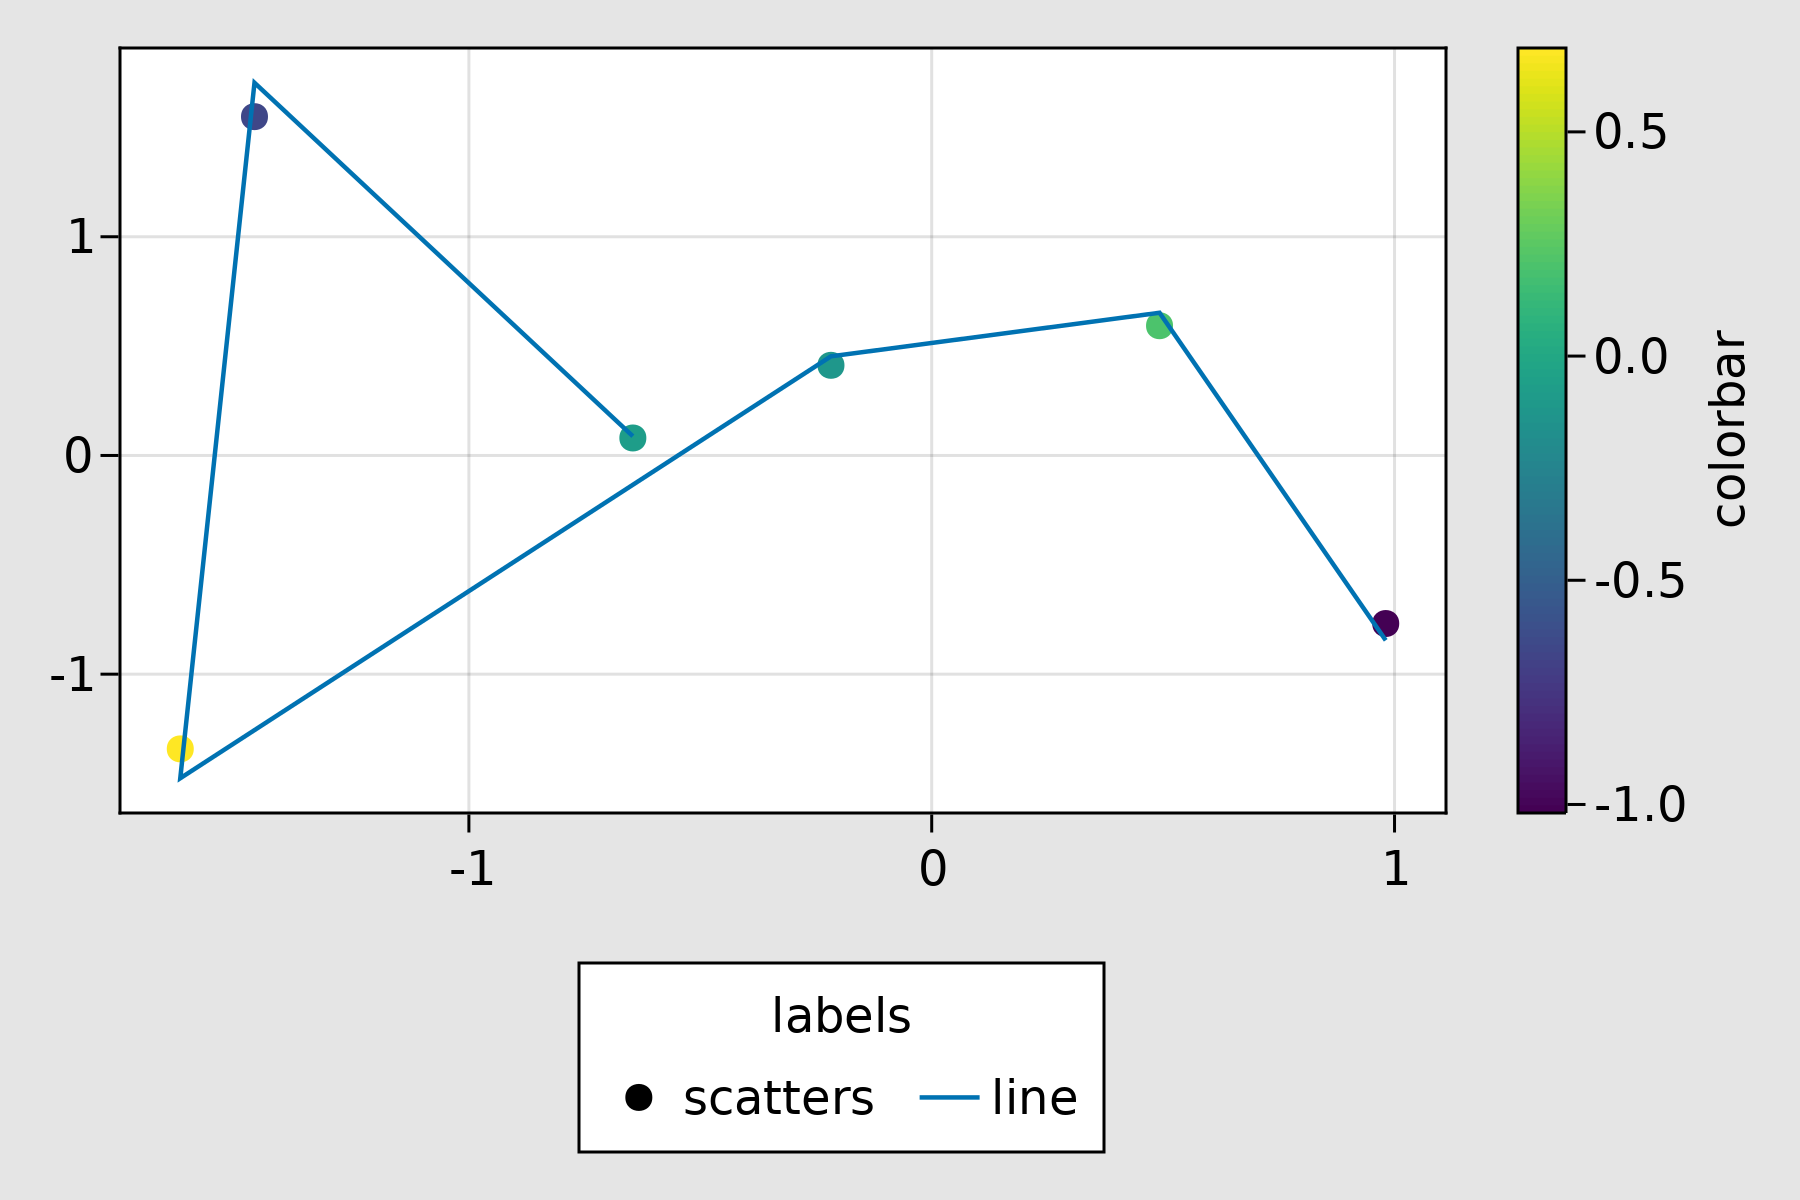
\includegraphics[width=0.6\textwidth,height=\textheight]{_build/im/JDS_first_layout_.png}
\caption{First Layout.}\label{fig:first_layout}
}
\end{figure}

Isso já parece bom, mas poderia ser melhor. Podemos corrigir problemas
de espaçamento usando as seguintes palavras-chave e métodos:

\begin{itemize}
\tightlist
\item
  \passthrough{\lstinline!figure\_padding=(left, right, bottom, top)!}
\item
  \passthrough{\lstinline!padding=(left, right, bottom, top)!}
\end{itemize}

Levar em consideração o tamanho real de uma
\passthrough{\lstinline!Legend!} ou \passthrough{\lstinline!Colorbar!} é
feito por:

\begin{quote}
\begin{itemize}
\tightlist
\item
  \passthrough{\lstinline!tellheight=true!} ou
  \passthrough{\lstinline!false!}
\item
  \passthrough{\lstinline!tellwidth=true!} ou
  \passthrough{\lstinline!false!}
\end{itemize}

\emph{Definir como \passthrough{\lstinline!true!} levará em consideração
o tamanho real (altura ou largura) para uma
\passthrough{\lstinline!Legend!} ou \passthrough{\lstinline!Colorbar!}}.
Consequentemente, as coisas serão redimensionadas de acordo.
\end{quote}

O espaço entre colunas e linhas é especificado como:

\begin{quote}
\begin{itemize}
\tightlist
\item
  \passthrough{\lstinline"colgap!(fig.layout, col, separation)"}
\item
  \passthrough{\lstinline"rowgap!(fig.layout, row, separation)"}
\end{itemize}

\emph{Column gap} (\passthrough{\lstinline"colgap!"}), se
\passthrough{\lstinline!col!} for fornecido, a lacuna será aplicada a
essa coluna específica. \emph{Row gap}
(\passthrough{\lstinline"rowgap!"}) , se a
\passthrough{\lstinline!linha!} for fornecido, a lacuna será aplicada a
essa linha específica.
\end{quote}

Além disso, veremos como colocar conteúdo nas \textbf{protrusões},
\emph{i.e.} o espaço reservado para título: \passthrough{\lstinline!x!}
e \passthrough{\lstinline!y!}; ou \passthrough{\lstinline!ticks!} ou
\passthrough{\lstinline!label!}. Fazemos isso plotando em
\passthrough{\lstinline!fig[i, j, protrusion]!} onde
\passthrough{\lstinline!protrusion!} pode ser
\passthrough{\lstinline!Left()!}, \passthrough{\lstinline!Right()!},
\passthrough{\lstinline!Bottom()!} e \passthrough{\lstinline!Top()!}, ou
para cada canto \passthrough{\lstinline!TopLeft()!},
\passthrough{\lstinline!TopRight()!},
\passthrough{\lstinline!BottomRight()!},
\passthrough{\lstinline!BottomLeft()!}. Veja abaixo como essas opções
estão sendo utilizadas:

\begin{lstlisting}[language=Julia]
function first_layout_fixed()
    seed!(123)
    x, y, z = randn(6), randn(6), randn(6)
    fig = Figure(figure_padding=(0, 3, 5, 2), resolution=(600, 400),
        backgroundcolor=:grey90, font="CMU Serif")
    ax = Axis(fig[1, 1], xlabel=L"x", ylabel=L"y",
        title="Layout example", backgroundcolor=:white)
    pltobj = scatter!(ax, x, y; color=z, label="scatters")
    lines!(ax, x, 1.1y, label="line")
    Legend(fig[2, 1:2], ax, "Labels", orientation=:horizontal,
        tellheight=true, titleposition=:left)
    Colorbar(fig[1, 2], pltobj, label="colorbar")
    # additional aesthetics
    Box(fig[1, 1, Right()], color=(:slateblue1, 0.35))
    Label(fig[1, 1, Right()], "protrusion", textsize=18,
        rotation=pi / 2, padding=(3, 3, 3, 3))
    Label(fig[1, 1, TopLeft()], "(a)", textsize=18, padding=(0, 3, 8, 0))
    colgap!(fig.layout, 5)
    rowgap!(fig.layout, 5)
    fig
end
first_layout_fixed()
\end{lstlisting}

\begin{figure}
\hypertarget{fig:first_layout_fixed}{%
\centering
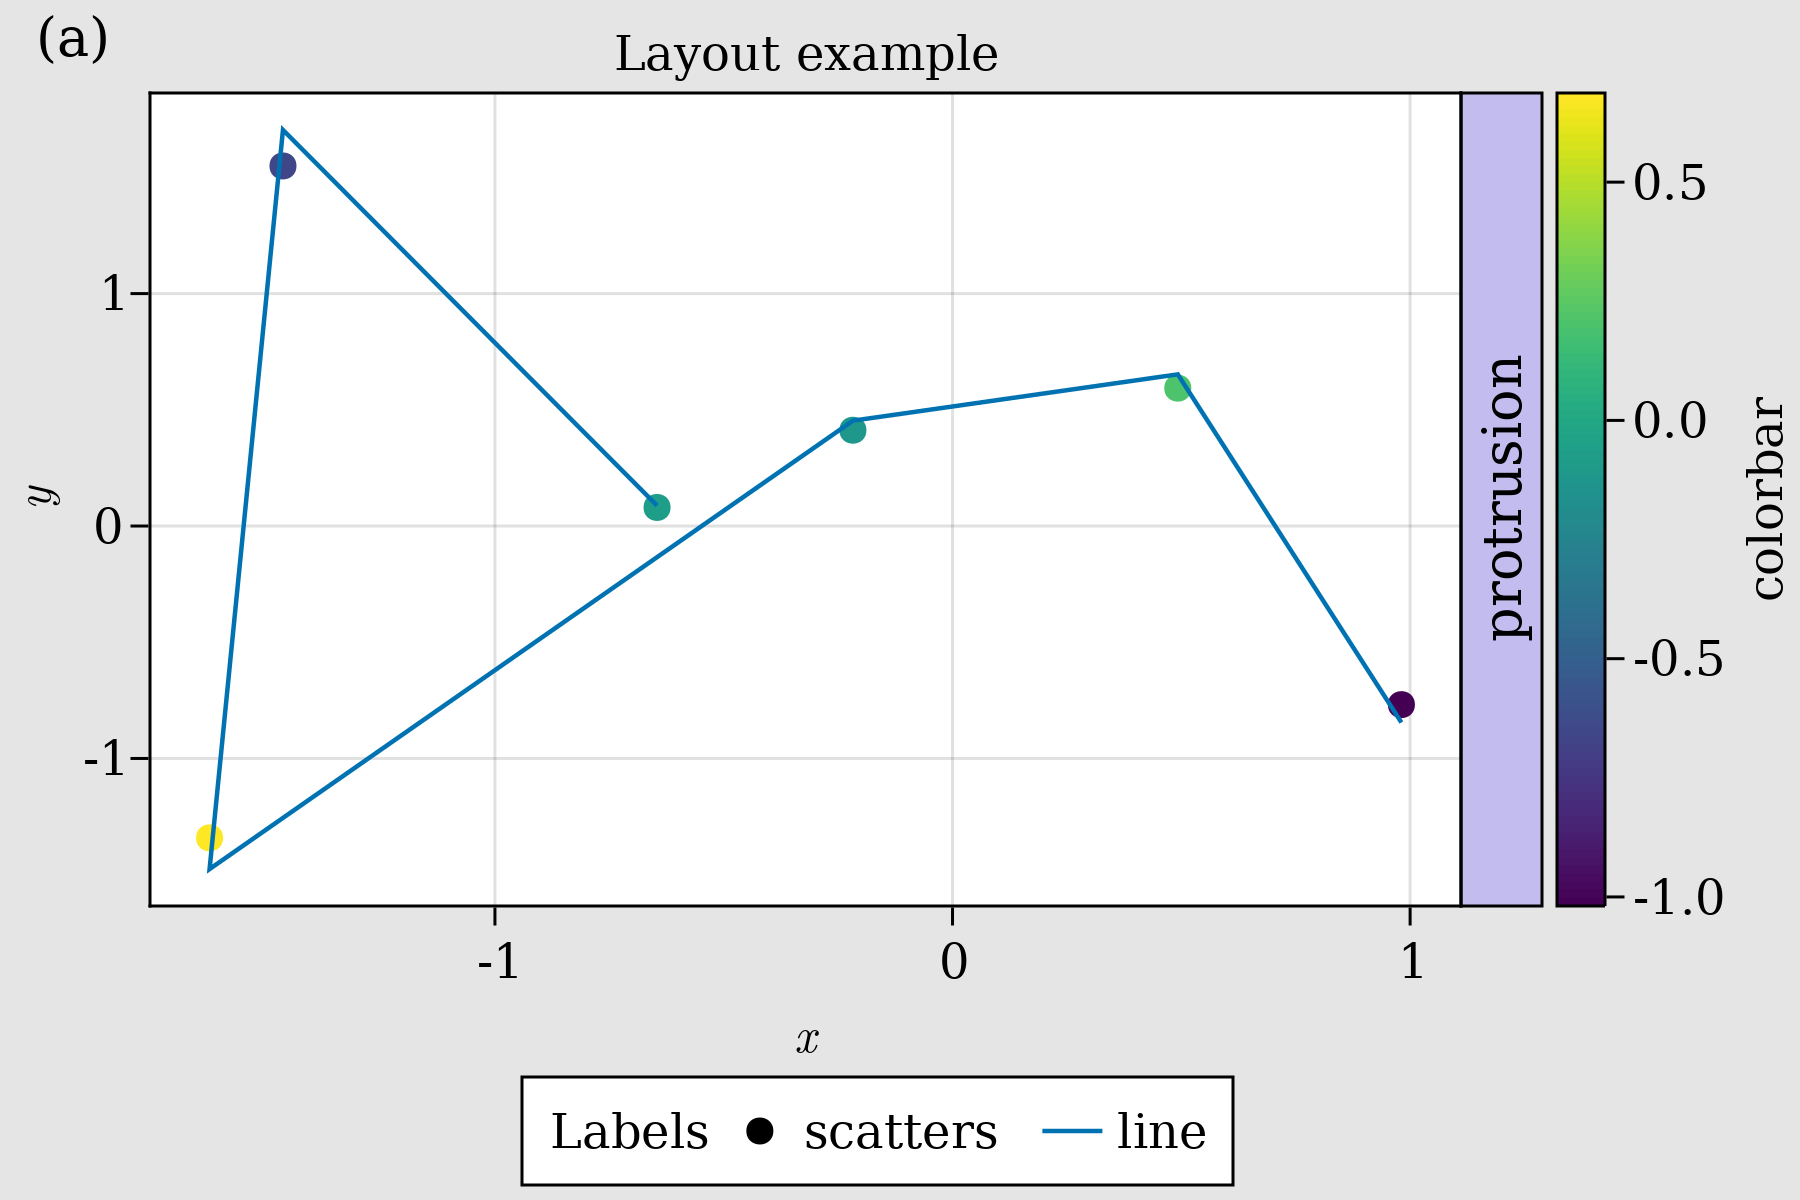
\includegraphics[width=0.6\textwidth,height=\textheight]{_build/im/JDS_first_layout_fixed_.png}
\caption{First Layout Fixed.}\label{fig:first_layout_fixed}
}
\end{figure}

Aqui, ter o rótulo \passthrough{\lstinline!(a)!} no
\passthrough{\lstinline!TopLeft()!} provavelmente não é necessário, isso
só fará sentido para mais de dois \emph{plots}. Para o nosso próximo
exemplo vamos continuar usando as ferramentas anteriores e mais algumas
para criar uma figura mais rica e complexa.

Você pode ocultar decorações e espinhas de eixos com:

\begin{quote}
\begin{itemize}
\tightlist
\item
  \passthrough{\lstinline"hidedecorations!(ax; kwargs...)"}
\item
  \passthrough{\lstinline"hidexdecorations!(ax; kwargs...)"}
\item
  \passthrough{\lstinline"hideydecorations!(ax; kwargs...)"}
\item
  \passthrough{\lstinline"hidespines!(ax; kwargs...)"}
\end{itemize}
\end{quote}

Lembre-se, sempre podemos pedir ajuda para ver que tipo de argumentos
podemos usar, por exemplo,

\begin{lstlisting}[language=Julia]
help(hidespines!)
\end{lstlisting}

\begin{lstlisting}[language=Output]
  hidespines!(la::Axis, spines::Symbol... = (:l, :r, :b, :t)...)

  Hide all specified axis spines. Hides all spines by default, otherwise
  choose with the symbols :l, :r, :b and :t.

  hidespines! has the following function signatures:

    (Vector, Vector)
    (Vector, Vector, Vector)
    (Matrix)

  Available attributes for Combined{Makie.MakieLayout.hidespines!} are:

  
\end{lstlisting}

Alternativamente, para decorações:

\begin{lstlisting}[language=Julia]
help(hidedecorations!)
\end{lstlisting}

\begin{lstlisting}[language=Output]
  hidedecorations!(la::Axis)

  Hide decorations of both x and y-axis: label, ticklabels, ticks and grid.

  hidedecorations! has the following function signatures:

    (Vector, Vector)
    (Vector, Vector, Vector)
    (Matrix)

  Available attributes for Combined{Makie.MakieLayout.hidedecorations!} are:

  
\end{lstlisting}

Para elementos que \textbf{você não deseja ocultar}, apenas passe-os com
\passthrough{\lstinline!false!}, ou seja,
\passthrough{\lstinline"hideydecorations!(ax; ticks=false, grid=false)"}.

A sincronização do seu \passthrough{\lstinline!Axis!} é feita via:

\begin{quote}
\begin{itemize}
\tightlist
\item
  \passthrough{\lstinline"linkaxes!"},
  \passthrough{\lstinline"linkyaxes!"} e
  \passthrough{\lstinline"linkxaxes!"}
\end{itemize}

Isso pode ser útil quando eixos compartilhados são desejados. Outra
maneira de obter eixos compartilhados será definindo
\passthrough{\lstinline"limites!"}.
\end{quote}

Definir limites de uma vez ou independentemente para cada eixo é feito
chamando

\begin{quote}
\begin{itemize}
\tightlist
\item
  \passthrough{\lstinline"limits!(ax; l, r, b, t)"}, onde
  \passthrough{\lstinline!l!} é esquerda, \passthrough{\lstinline!r!}
  direita, \passthrough{\lstinline!b!} inferior e
  \passthrough{\lstinline!t!} superior.
\end{itemize}

Você também pode fazer \passthrough{\lstinline"ylims!(low, high)"} ou
\passthrough{\lstinline"xlims!(low, high)"}, e até mesmo abrir fazendo
\passthrough{\lstinline"ylims!(low=0)"} ou
\passthrough{\lstinline"xlims!(high=1)"}.
\end{quote}

Agora, o exemplo:

\begin{lstlisting}[language=Julia]
function complex_layout_double_axis()
    seed!(123)
    x = LinRange(0, 1, 10)
    y = LinRange(0, 1, 10)
    z = rand(10, 10)
    fig = Figure(resolution=(600, 400), font="CMU Serif", backgroundcolor=:grey90)
    ax1 = Axis(fig, xlabel=L"x", ylabel=L"y")
    ax2 = Axis(fig, xlabel=L"x")
    heatmap!(ax1, x, y, z; colorrange=(0, 1))
    series!(ax2, abs.(z[1:4, :]); labels=["lab $i" for i = 1:4], color=:Set1_4)
    hm = scatter!(10x, y; color=z[1, :], label="dots", colorrange=(0, 1))
    hideydecorations!(ax2, ticks=false, grid=false)
    linkyaxes!(ax1, ax2)
    #layout
    fig[1, 1] = ax1
    fig[1, 2] = ax2
    Label(fig[1, 1, TopLeft()], "(a)", textsize=18, padding=(0, 6, 8, 0))
    Label(fig[1, 2, TopLeft()], "(b)", textsize=18, padding=(0, 6, 8, 0))
    Colorbar(fig[2, 1:2], hm, label="colorbar", vertical=false, flipaxis=false)
    Legend(fig[1, 3], ax2, "Legend")
    colgap!(fig.layout, 5)
    rowgap!(fig.layout, 5)
    fig
end
complex_layout_double_axis()
\end{lstlisting}

\begin{figure}
\hypertarget{fig:complex_layout_double_axis}{%
\centering
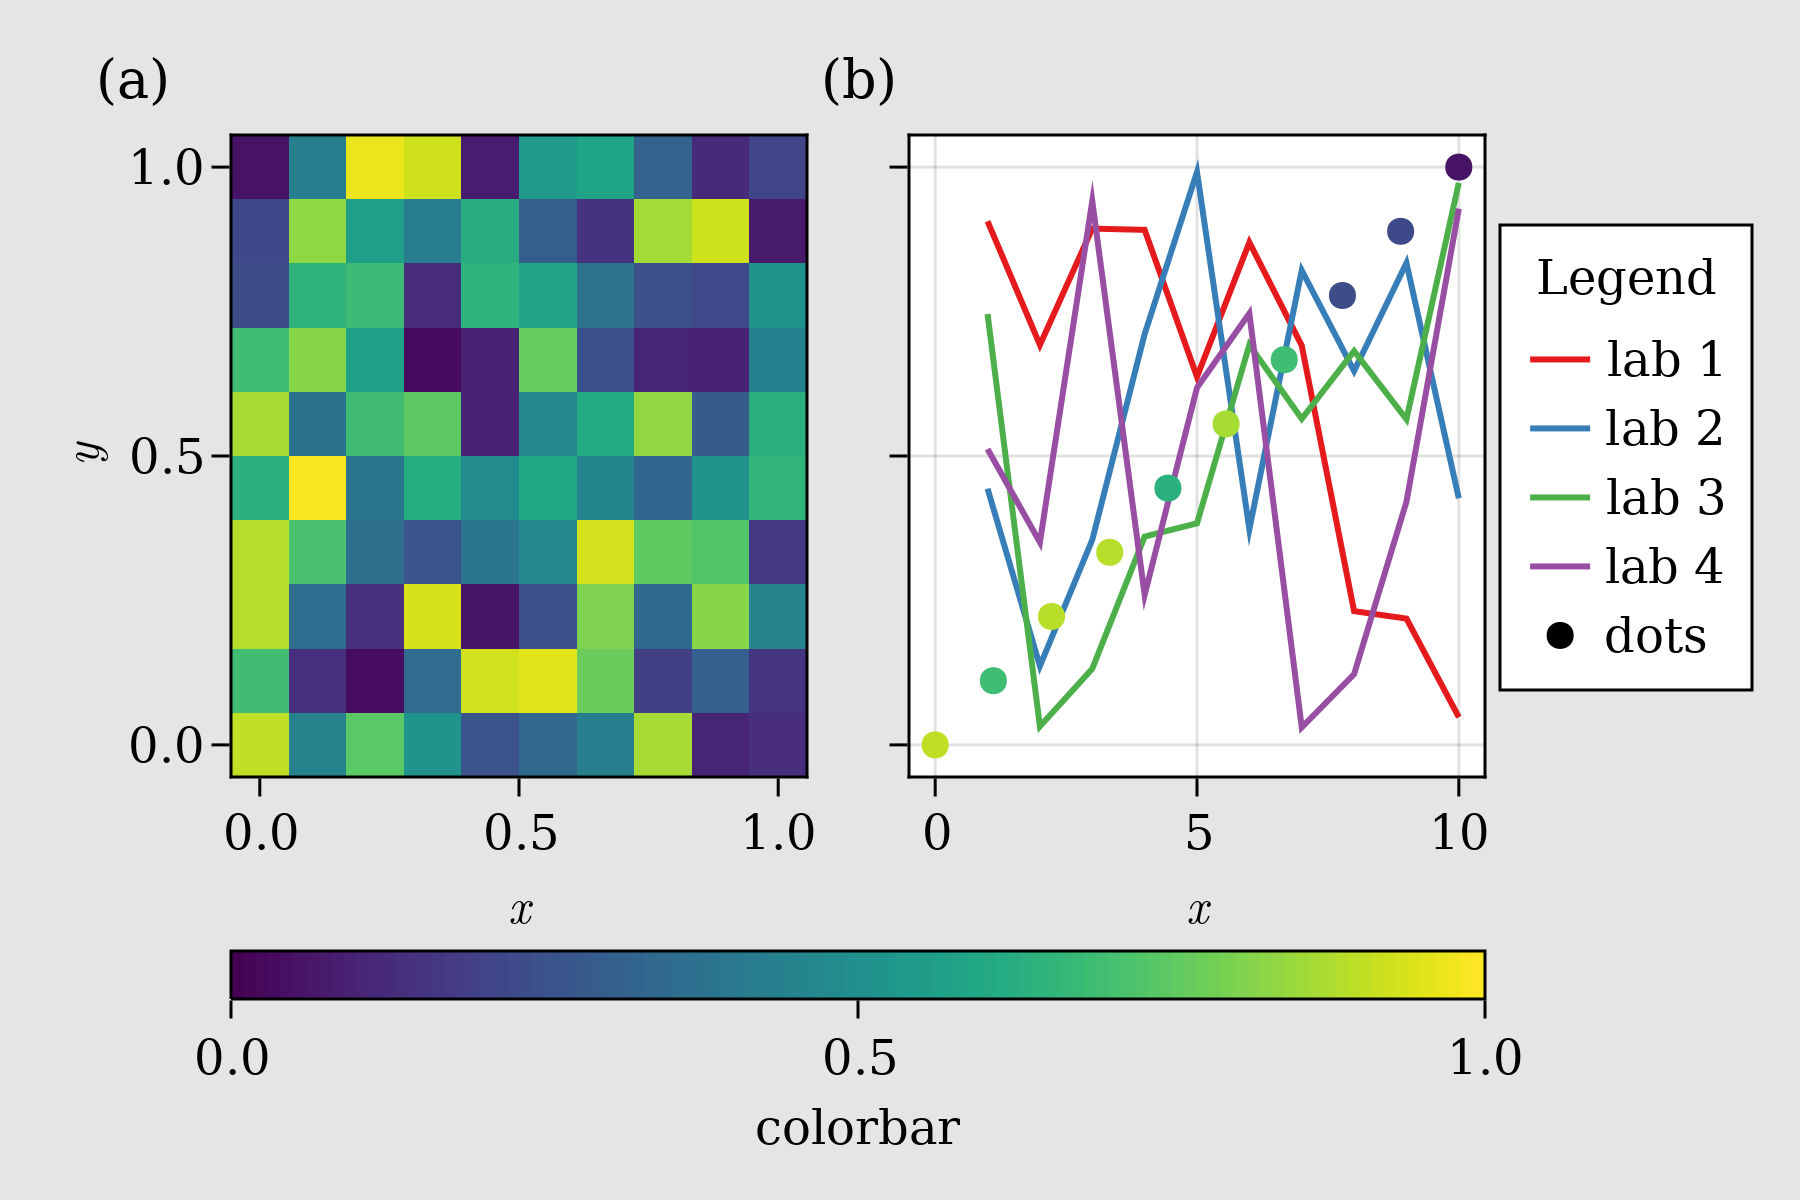
\includegraphics[width=0.6\textwidth,height=\textheight]{_build/im/JDS_complex_layout_double_axis_.png}
\caption{Complex layout double
axis.}\label{fig:complex_layout_double_axis}
}
\end{figure}

Então, agora nosso \passthrough{\lstinline!Colorbar!} precisa ser
horizontal e as marcações da barra precisam estar na parte inferior.
Isso é feito configurando \passthrough{\lstinline!vertical=false!} e
\passthrough{\lstinline!flipaxis=false!}. Além disso, observe que
podemos chamar muitos \passthrough{\lstinline!Axis!} em
\passthrough{\lstinline!fig!}, ou mesmo
\passthrough{\lstinline!Colorbar!} e \passthrough{\lstinline!Legend!}, e
depois construir o layout.

Outro layout comum é uma grade de quadrados para mapas de calor:

\begin{lstlisting}[language=Julia]
function squares_layout()
    seed!(123)
    letters = reshape(collect('a':'d'), (2, 2))
    fig = Figure(resolution=(600, 400), fontsize=14, font="CMU Serif",
        backgroundcolor=:grey90)
    axs = [Axis(fig[i, j], aspect=DataAspect()) for i = 1:2, j = 1:2]
    hms = [heatmap!(axs[i, j], randn(10, 10), colorrange=(-2, 2))
           for i = 1:2, j = 1:2]
    Colorbar(fig[1:2, 3], hms[1], label="colorbar")
    [Label(fig[i, j, TopLeft()], "($(letters[i, j]))", textsize=16,
        padding=(-2, 0, -20, 0)) for i = 1:2, j = 1:2]
    colgap!(fig.layout, 5)
    rowgap!(fig.layout, 5)
    fig
end
squares_layout()
\end{lstlisting}

\begin{figure}
\hypertarget{fig:squares_layout}{%
\centering
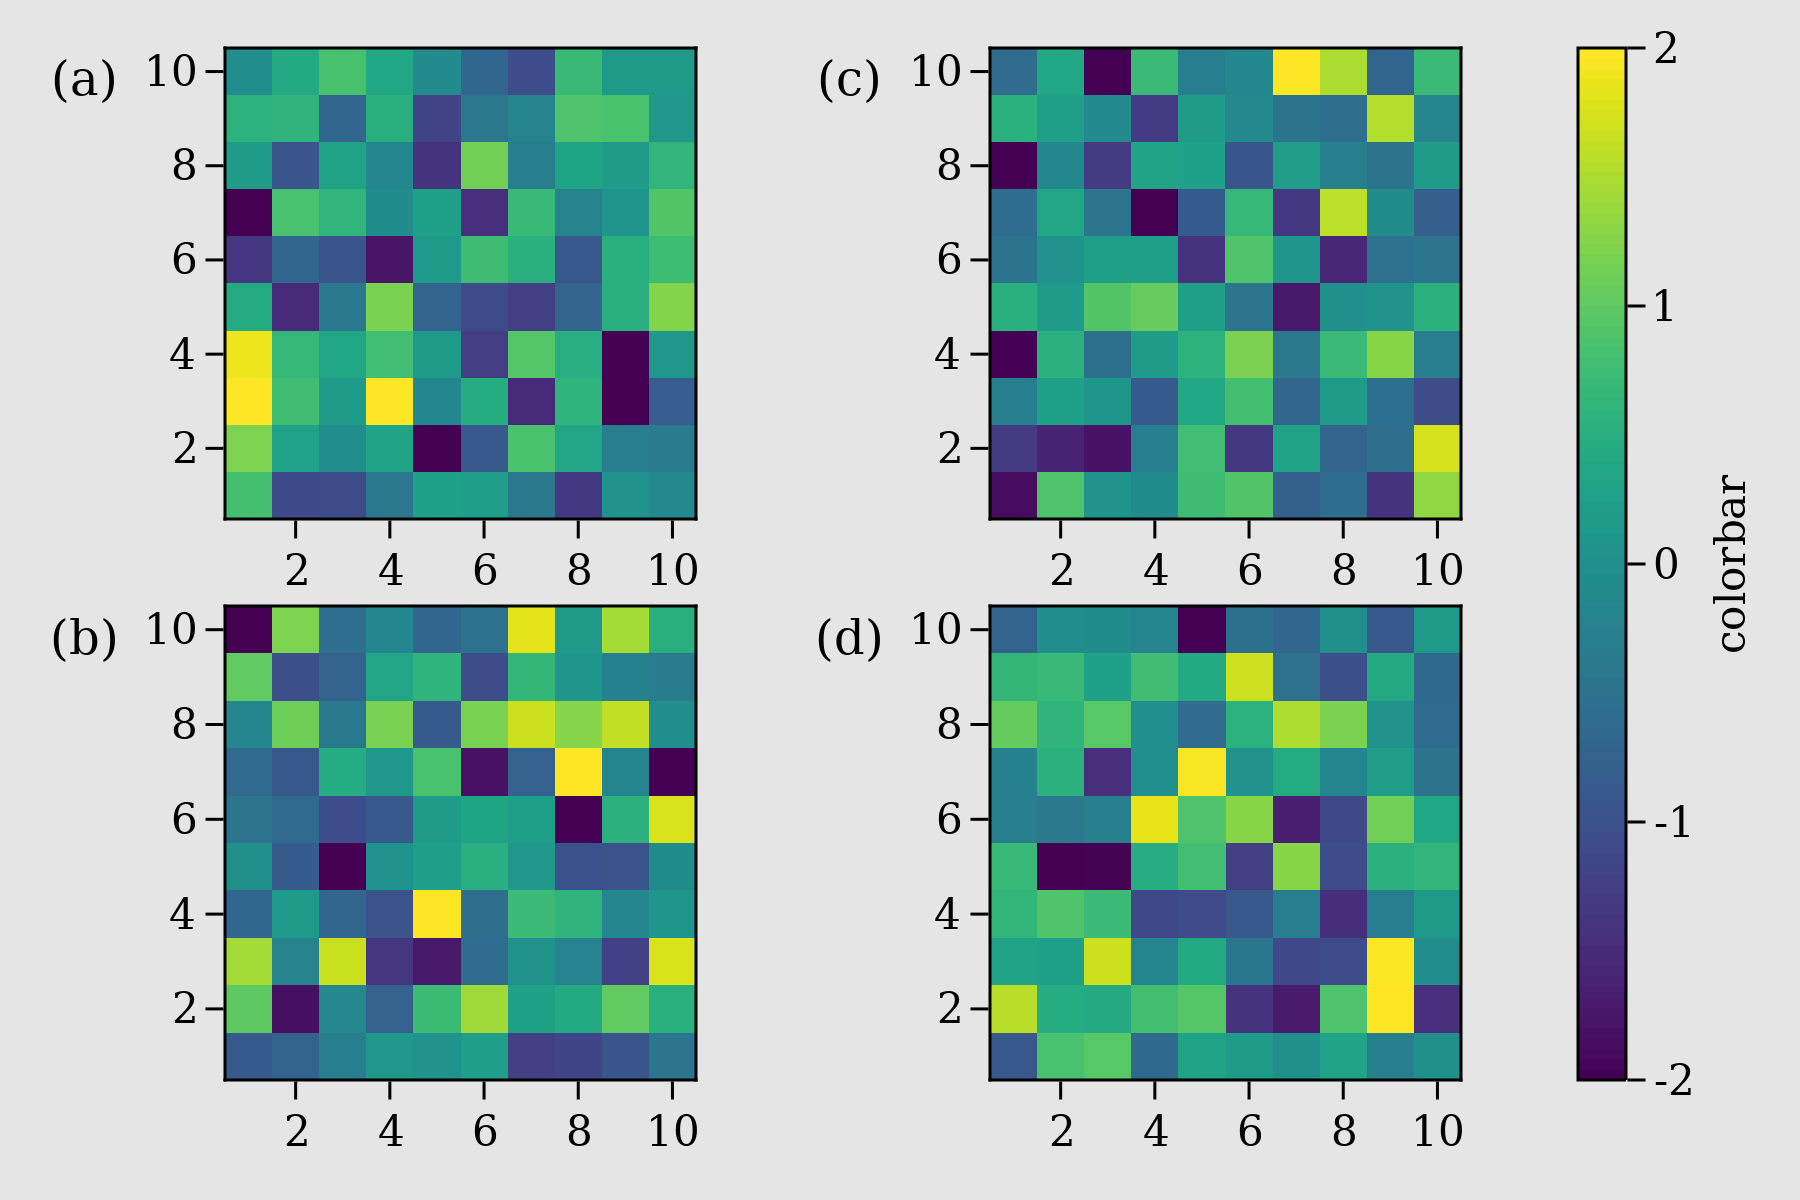
\includegraphics[width=0.6\textwidth,height=\textheight]{_build/im/JDS_squares_layout_.png}
\caption{Squares layout.}\label{fig:squares_layout}
}
\end{figure}

onde todos os rótulos estão em \textbf{protrusões} e cada
\passthrough{\lstinline!Axis!} tem uma razão
\passthrough{\lstinline!AspectData()!}. A
\passthrough{\lstinline!Colorbar!} está localizada na terceira coluna e
se expande da linha 1 até a linha 2.

O próximo caso usa o chamado \textbf{modo de alinhamento}
\passthrough{\lstinline!Mixed()!}, o que é especialmente útil ao lidar
com grandes espaços vazios entre \passthrough{\lstinline!Axis!} devido a
tiques longos. Ainda, o módulo \passthrough{\lstinline!Dates!} da
biblioteca padrão de Julia será necessário para esse exemplo.

\begin{lstlisting}
using Dates
\end{lstlisting}

\begin{lstlisting}[language=Julia]
function mixed_mode_layout()
    seed!(123)
    longlabels = ["$(today() - Day(1))", "$(today())", "$(today() + Day(1))"]
    fig = Figure(resolution=(600, 400), fontsize=12,
        backgroundcolor=:grey90, font="CMU Serif")
    ax1 = Axis(fig[1, 1])
    ax2 = Axis(fig[1, 2], xticklabelrotation=pi / 2, alignmode=Mixed(bottom=0),
        xticks=([1, 5, 10], longlabels))
    ax3 = Axis(fig[2, 1:2])
    ax4 = Axis(fig[3, 1:2])
    axs = [ax1, ax2, ax3, ax4]
    [lines!(ax, 1:10, rand(10)) for ax in axs]
    hidexdecorations!(ax3; ticks=false, grid=false)
    Box(fig[2:3, 1:2, Right()], color=(:slateblue1, 0.35))
    Label(fig[2:3, 1:2, Right()], "protrusion", rotation=pi / 2, textsize=14,
        padding=(3, 3, 3, 3))
    Label(fig[1, 1:2, Top()], "Mixed alignmode", textsize=16,
        padding=(0, 0, 15, 0))
    colsize!(fig.layout, 1, Auto(2))
    rowsize!(fig.layout, 2, Auto(0.5))
    rowsize!(fig.layout, 3, Auto(0.5))
    rowgap!(fig.layout, 1, 15)
    rowgap!(fig.layout, 2, 0)
    colgap!(fig.layout, 5)
    fig
end
mixed_mode_layout()
\end{lstlisting}

\begin{figure}
\hypertarget{fig:mixed_mode_layout}{%
\centering
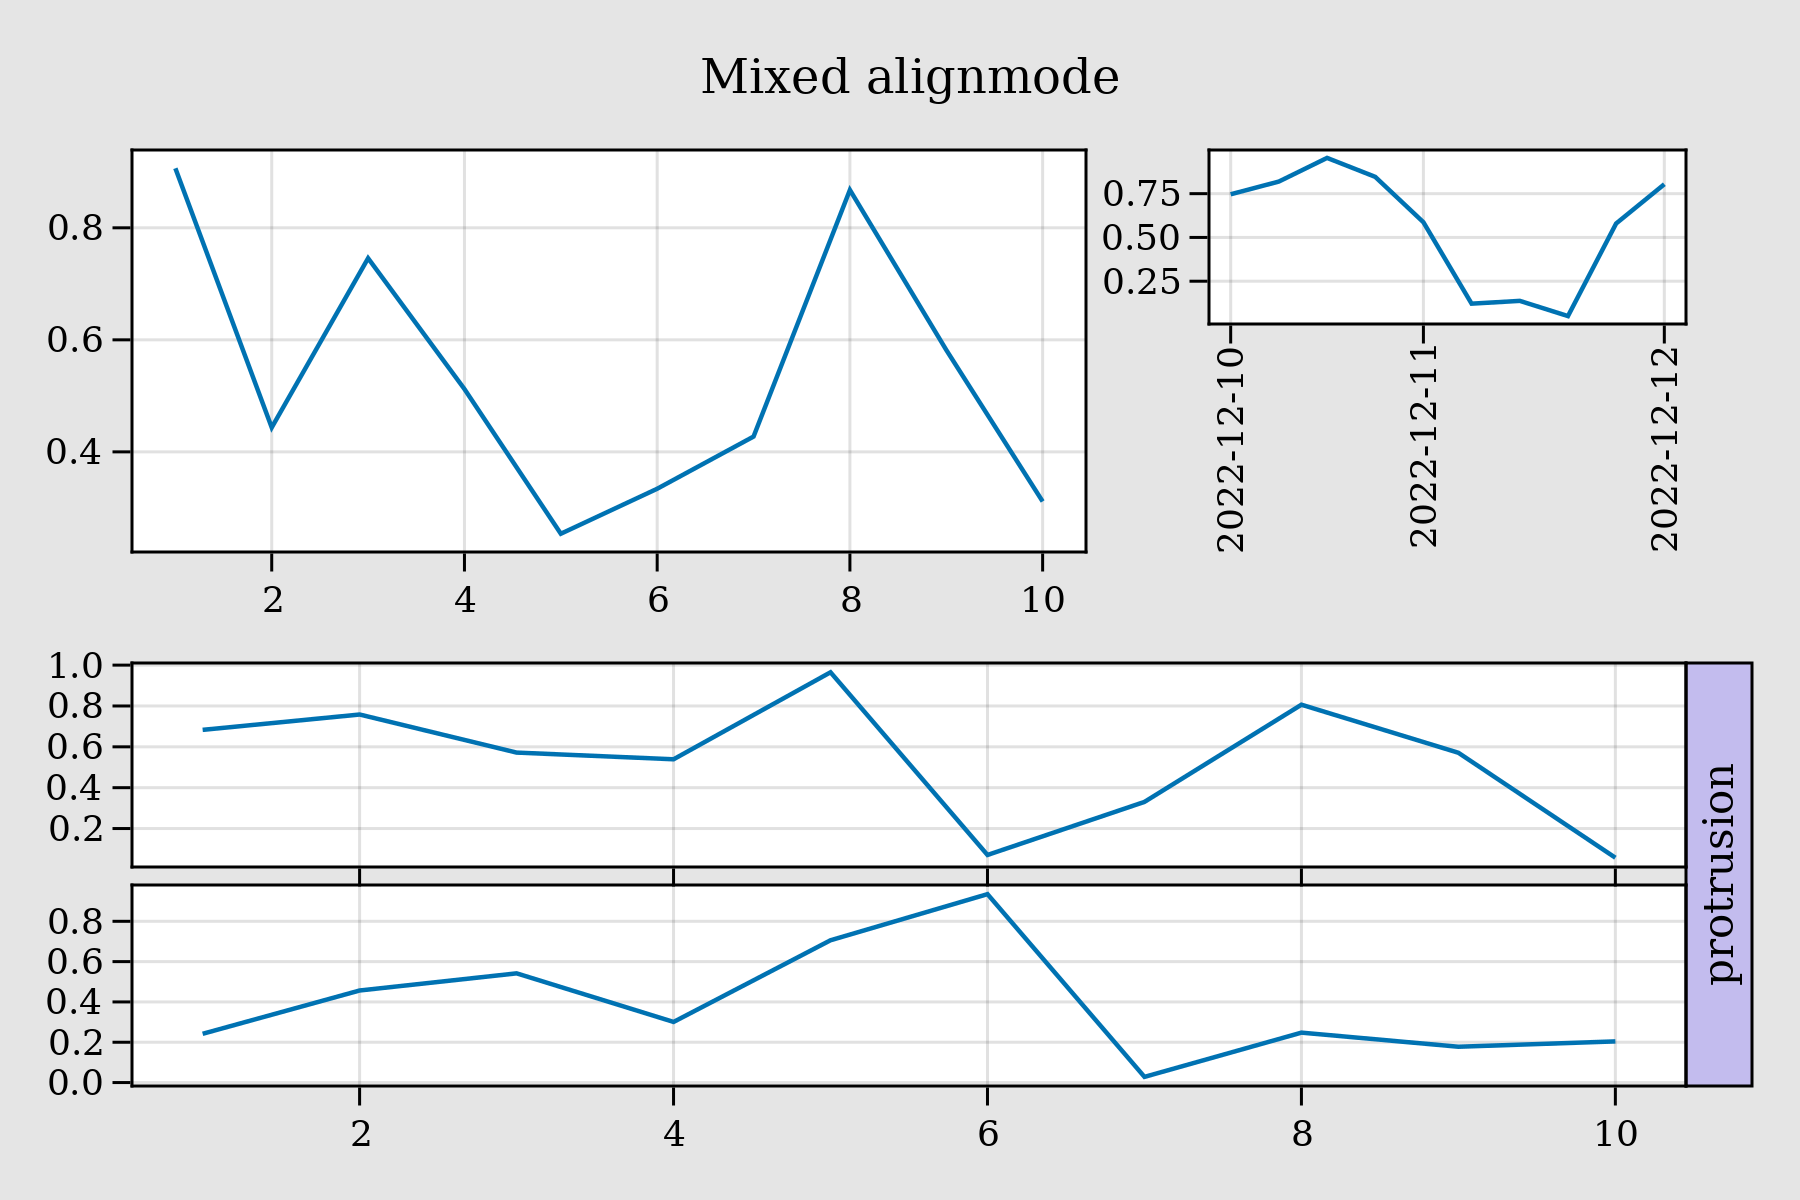
\includegraphics[width=0.6\textwidth,height=\textheight]{_build/im/JDS_mixed_mode_layout_.png}
\caption{Mixed mode layout.}\label{fig:mixed_mode_layout}
}
\end{figure}

Aqui, o argumento \passthrough{\lstinline!alignmode=Mixed(bottom=0)!}
desloca a caixa delimitadora para a parte inferior, de forma a alinhar
com o painel à esquerda preenchendo o espaço.

Também, veja como \passthrough{\lstinline"colsize!"} e
\passthrough{\lstinline"rowsize!"} estão sendo usados para diferentes
colunas e linhas. Você também pode colocar um número ao invés de
\passthrough{\lstinline!Auto()!} mas então tudo vai ser corrigido. E,
além disso, pode-se também dar um \passthrough{\lstinline!height!} ou
\passthrough{\lstinline!width!} ao definir o
\passthrough{\lstinline!Axis!}, como em
\passthrough{\lstinline!Axis(fig, heigth=50)!} que será corrigido
também.

\hypertarget{axis-aninhado-subplots}{%
\subsection{\texorpdfstring{\texttt{Axis} aninhado
(\emph{subplots})}{Axis aninhado (subplots)}}\label{axis-aninhado-subplots}}

Também é possível definir um conjunto de \passthrough{\lstinline!Axis!}
(\emph{subplots}) explicitamente e use-o para construir uma figura
principal com várias linhas e colunas. Por exemplo, o seguinte é um
arranjo ``complicado'' de \passthrough{\lstinline!Axis!}:

\begin{lstlisting}[language=Julia]
function nested_sub_plot!(fig)
    color = rand(RGBf)
    ax1 = Axis(fig[1, 1], backgroundcolor=(color, 0.25))
    ax2 = Axis(fig[1, 2], backgroundcolor=(color, 0.25))
    ax3 = Axis(fig[2, 1:2], backgroundcolor=(color, 0.25))
    ax4 = Axis(fig[1:2, 3], backgroundcolor=(color, 0.25))
    return (ax1, ax2, ax3, ax4)
end
\end{lstlisting}

que, quando usado para construir uma figura mais complexa fazendo várias
chamadas, obtemos:

\begin{lstlisting}[language=Julia]
function main_figure()
    fig = Figure()
    Axis(fig[1, 1])
    nested_sub_plot!(fig[1, 2])
    nested_sub_plot!(fig[1, 3])
    nested_sub_plot!(fig[2, 1:3])
    fig
end
main_figure()
\end{lstlisting}

\begin{figure}
\hypertarget{fig:main_figure}{%
\centering
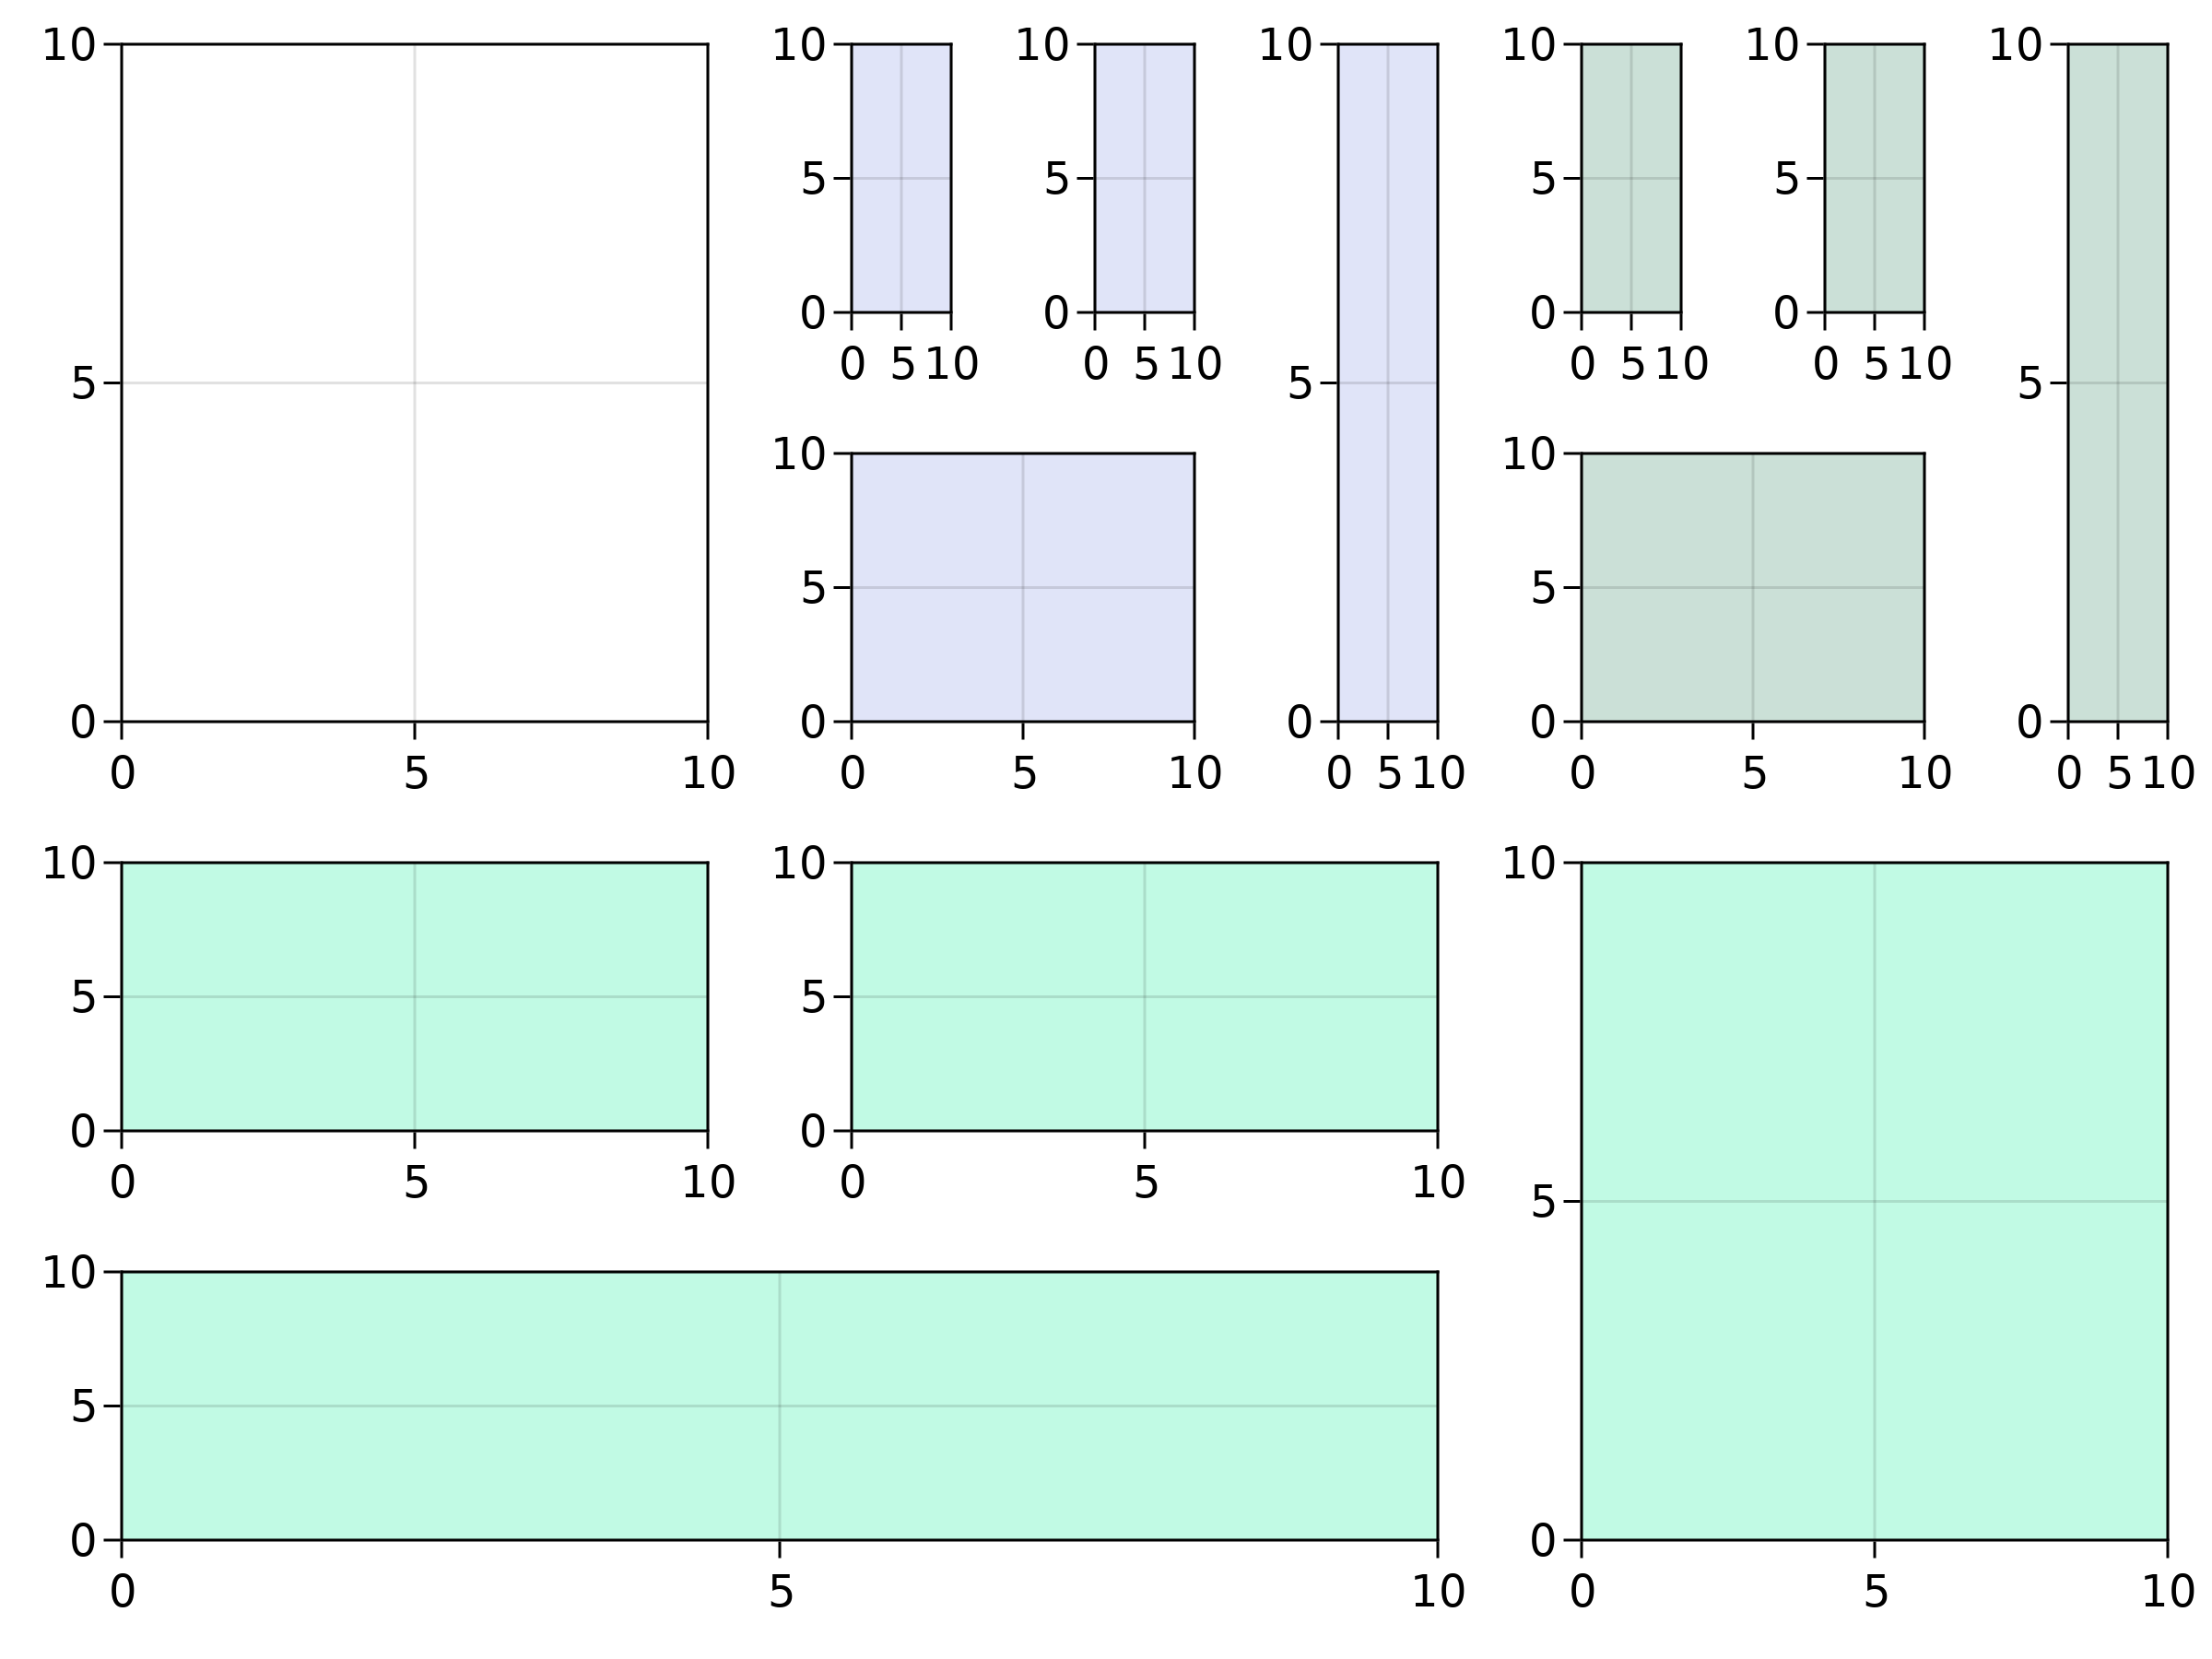
\includegraphics[width=0.6\textwidth,height=\textheight]{_build/im/JDS_main_figure_.png}
\caption{Main figure.}\label{fig:main_figure}
}
\end{figure}

Observe que diferentes funções de \emph{subplot} podem ser chamadas
aqui. Também, cada \passthrough{\lstinline!Axis!} aqui é uma parte
independente de \passthrough{\lstinline!Figure!}. Então, se você
precisar fazer alguma operação \passthrough{\lstinline"rowgap!"} ou
\passthrough{\lstinline"colsize!"}, você precisará fazê-lo em cada um
deles de forma independente ou em todos eles juntos.

Para \passthrough{\lstinline!Axis!} (\emph{subplots}) agrupados podemos
usar \passthrough{\lstinline!GridLayout()!} que, então, poderia ser
usado para compor um \passthrough{\lstinline!Figure!}.

\hypertarget{gridlayout-aninhado}{%
\subsection{GridLayout aninhado}\label{gridlayout-aninhado}}

Ao usar o \passthrough{\lstinline!GridLayout()!} podemos agrupar
\emph{subplots}, permitindo mais liberdade na construção de figuras
complexas. Aqui, usando nosso
\passthrough{\lstinline"nested\_sub\_plot!"} anterior, definimos três
subgrupos e um \passthrough{\lstinline!Axis!} normal:

\begin{lstlisting}[language=Julia]
function nested_Grid_Layouts()
    fig = Figure(backgroundcolor=RGBf(0.96, 0.96, 0.96))
    ga = fig[1, 1] = GridLayout()
    gb = fig[1, 2] = GridLayout()
    gc = fig[1, 3] = GridLayout()
    gd = fig[2, 1:3] = GridLayout()
    gA = Axis(ga[1, 1])
    nested_sub_plot!(gb)
    axsc = nested_sub_plot!(gc)
    nested_sub_plot!(gd)
    [hidedecorations!(axsc[i], grid=false, ticks=false) for i = 1:length(axsc)]
    colgap!(gc, 5)
    rowgap!(gc, 5)
    rowsize!(fig.layout, 2, Auto(0.5))
    colsize!(fig.layout, 1, Auto(0.5))
    fig
end
nested_Grid_Layouts()
\end{lstlisting}

\begin{figure}
\hypertarget{fig:nested_Grid_Layouts}{%
\centering
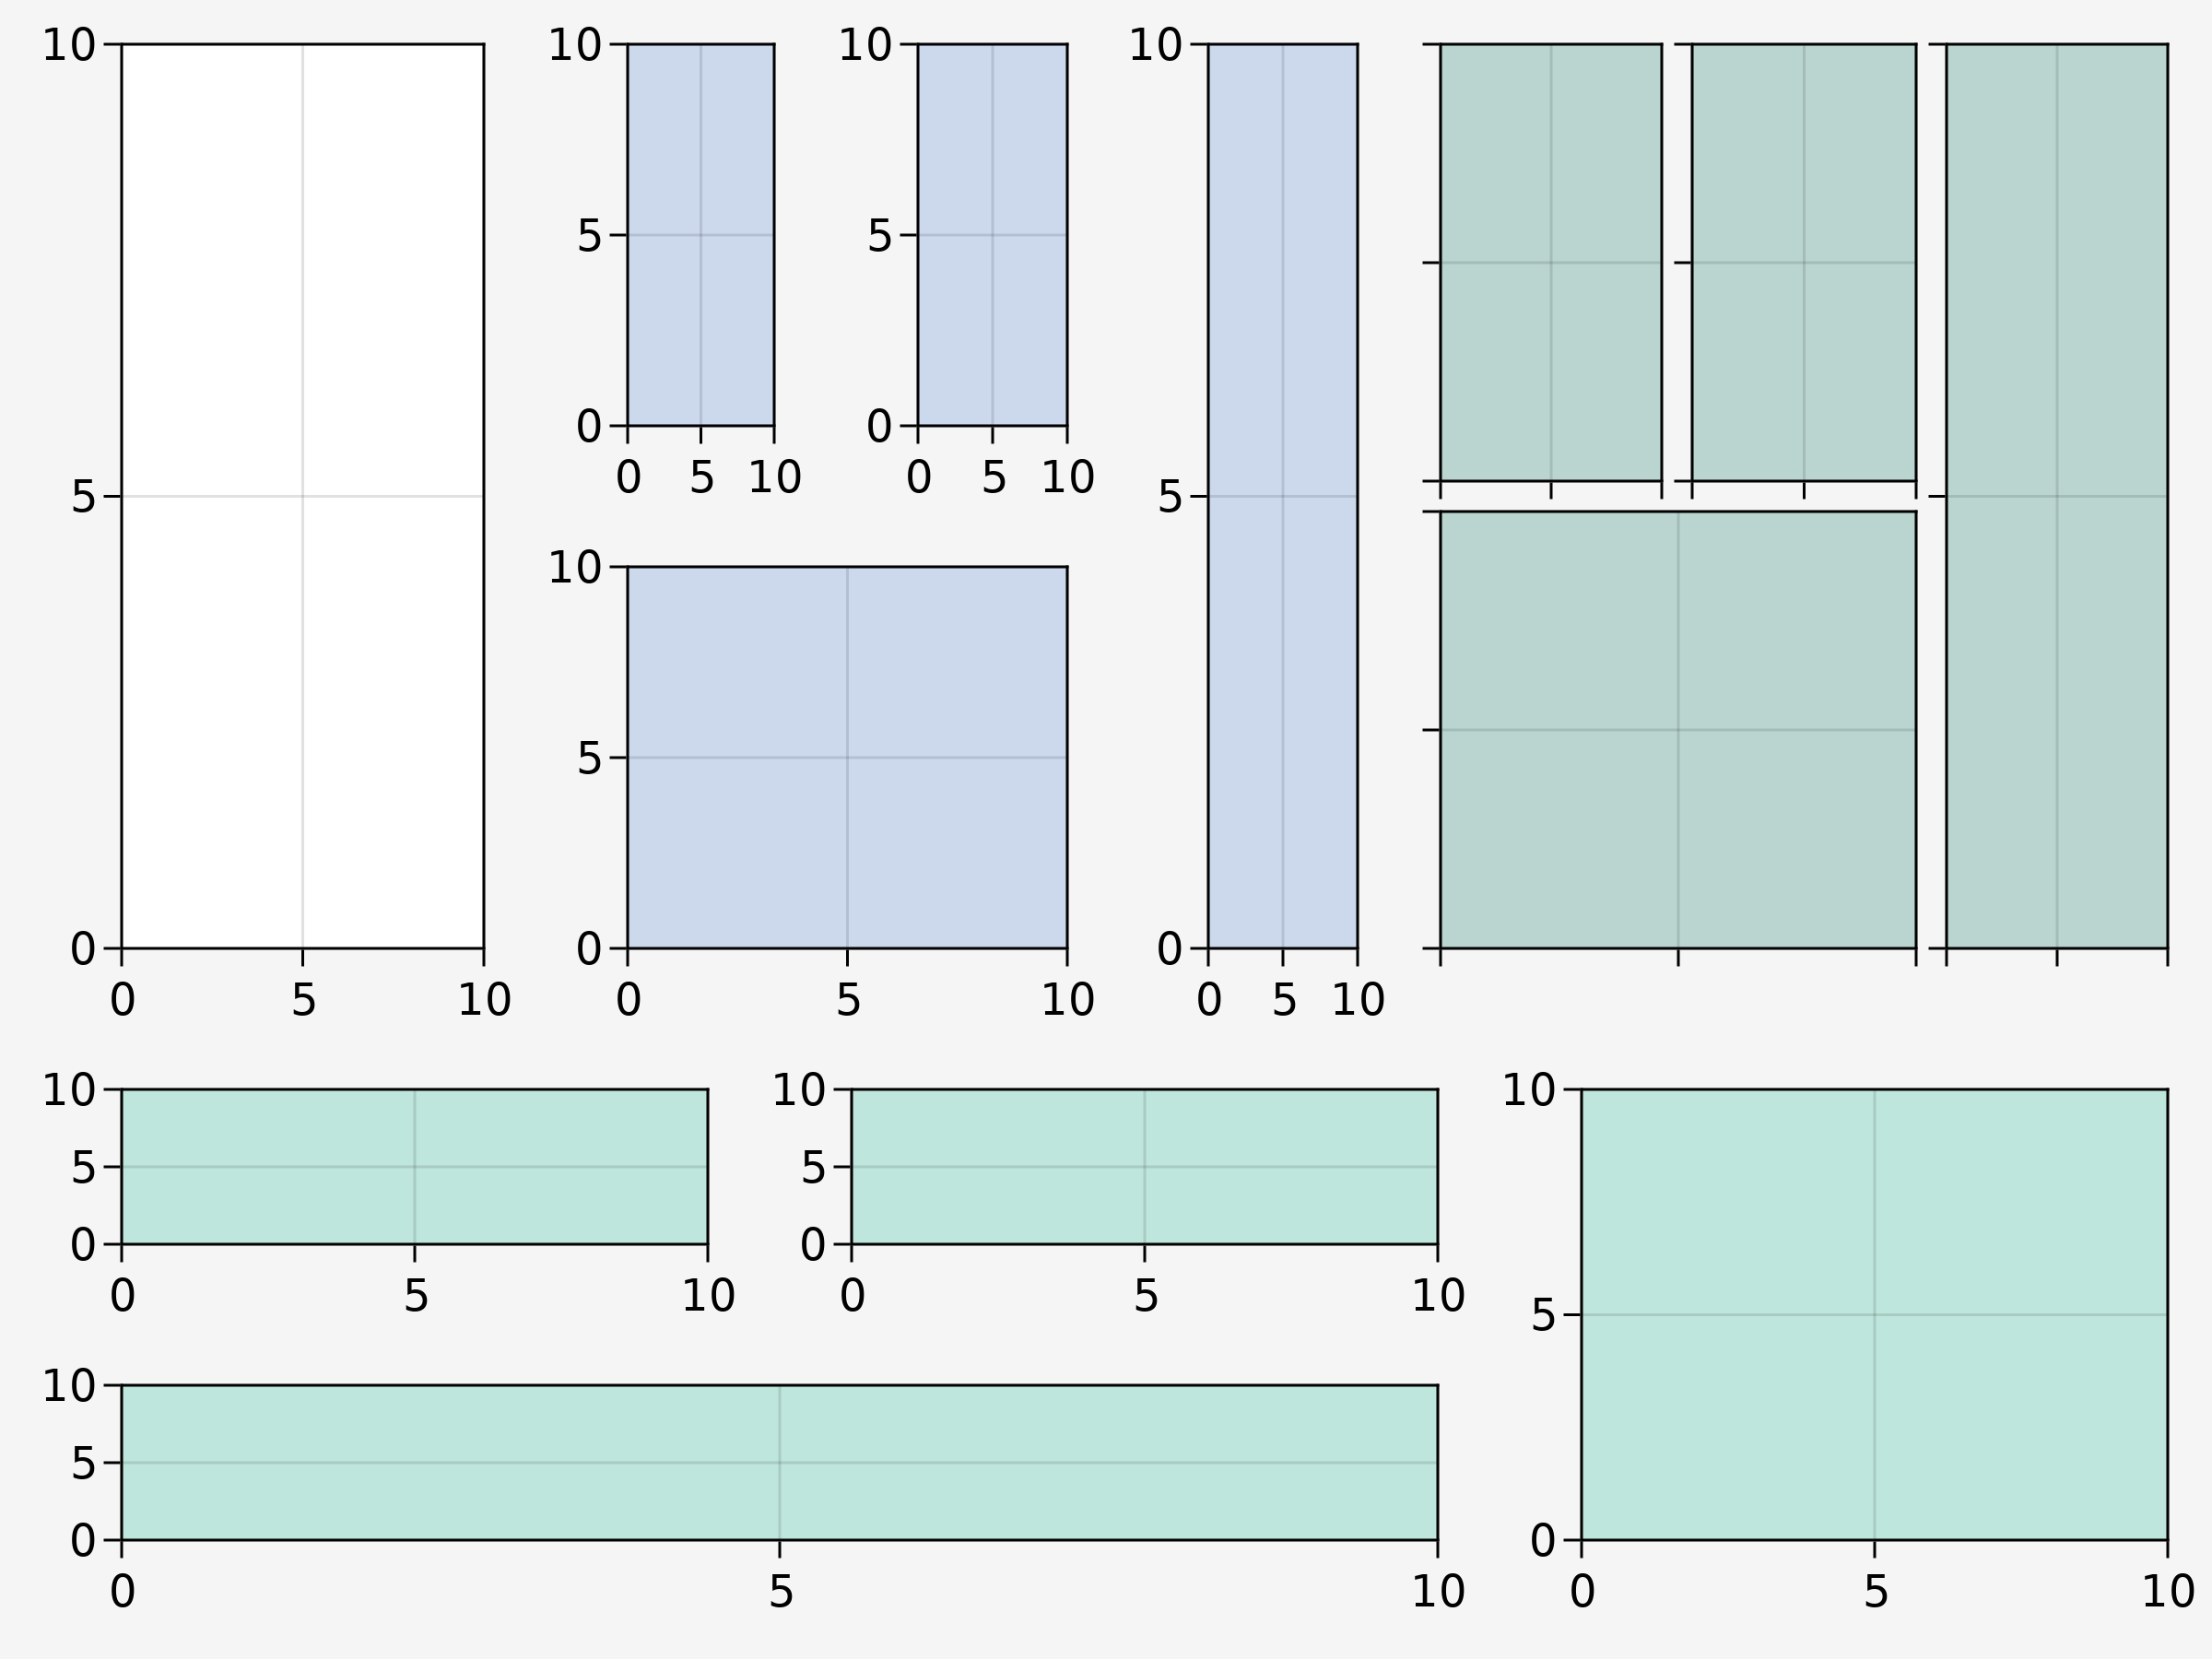
\includegraphics[width=0.6\textwidth,height=\textheight]{_build/im/JDS_nested_Grid_Layouts_.png}
\caption{Nested Grid Layouts.}\label{fig:nested_Grid_Layouts}
}
\end{figure}

Agora, usando \passthrough{\lstinline"rowgap!"} ou
\passthrough{\lstinline"colsize!"} sobre cada grupo é possível
\passthrough{\lstinline"rowsize!, colsize!"} também pode ser aplicado ao
conjunto de \passthrough{\lstinline!GridLayout()!}.

\hypertarget{plots-inset}{%
\subsection{\texorpdfstring{\emph{Plots}
\texttt{inset}}{Plots inset}}\label{plots-inset}}

Atualmente, fazer gráficos \passthrough{\lstinline!inset!} é um pouco
complicado. Aqui, mostramos duas maneiras possíveis de fazer isso
definindo inicialmente as funções auxiliares. A primeira é fazendo um
\passthrough{\lstinline!BBox!}, que fica em todo o espaço
\passthrough{\lstinline!Figure!}:

\begin{lstlisting}[language=Julia]
function add_box_inset(fig; left=100, right=250, bottom=200, top=300,
    bgcolor=:grey90)
    inset_box = Axis(fig, bbox=BBox(left, right, bottom, top),
        xticklabelsize=12, yticklabelsize=12, backgroundcolor=bgcolor)
    # bring content upfront
    translate!(inset_box.scene, 0, 0, 10)
    elements = keys(inset_box.elements)
    filtered = filter(ele -> ele != :xaxis && ele != :yaxis, elements)
    foreach(ele -> translate!(inset_box.elements[ele], 0, 0, 9), filtered)
    return inset_box
end
\end{lstlisting}

Então, o \passthrough{\lstinline!inset!} é feito facilmente, como em:

\begin{lstlisting}[language=Julia]
function figure_box_inset()
    fig = Figure(resolution=(600, 400))
    ax = Axis(fig[1, 1], backgroundcolor=:white)
    inset_ax1 = add_box_inset(fig; left=100, right=250, bottom=200, top=300,
        bgcolor=:grey90)
    inset_ax2 = add_box_inset(fig; left=500, right=600, bottom=100, top=200,
        bgcolor=(:white, 0.65))
    lines!(ax, 1:10)
    lines!(inset_ax1, 1:10)
    scatter!(inset_ax2, 1:10, color=:black)
    fig
end
figure_box_inset()
\end{lstlisting}

\begin{figure}
\hypertarget{fig:figure_box_inset}{%
\centering
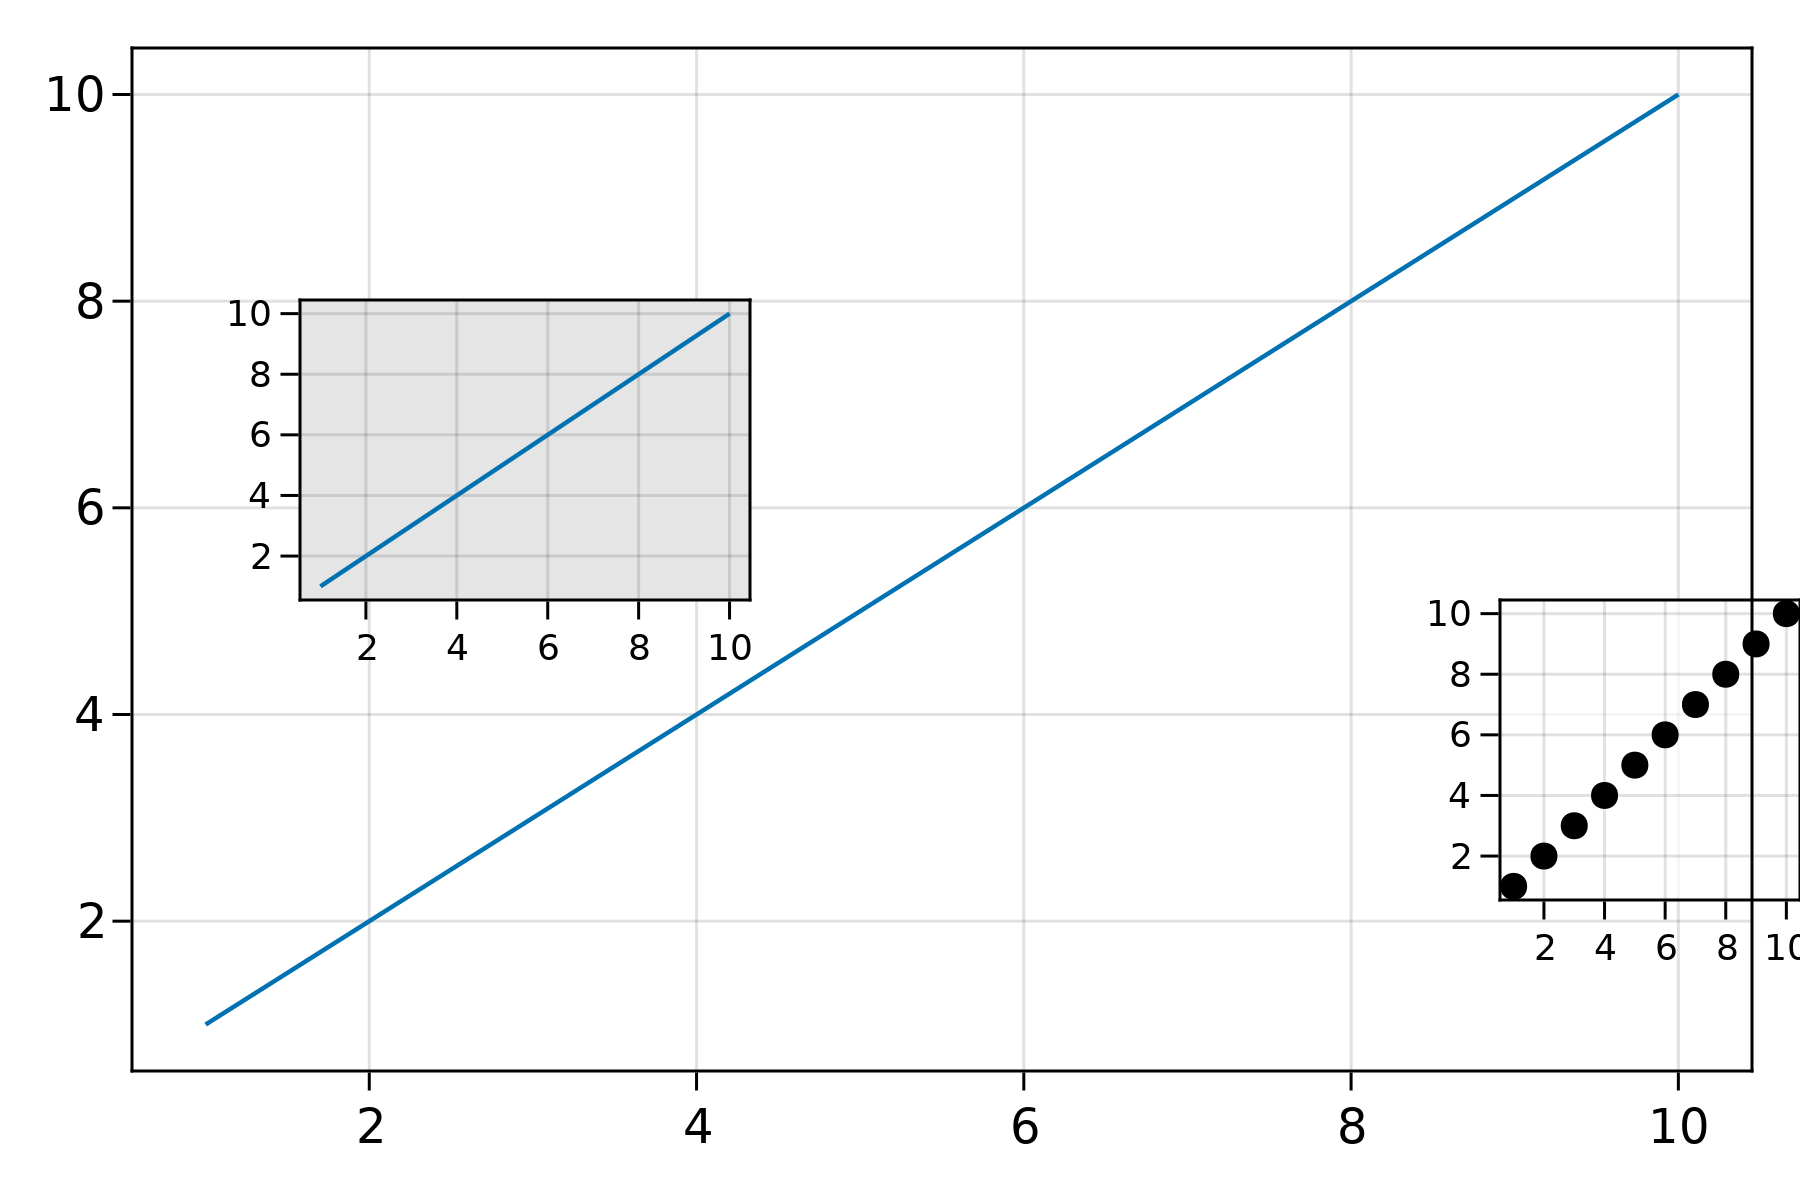
\includegraphics[width=0.6\textwidth,height=\textheight]{_build/im/JDS_figure_box_inset_.png}
\caption{Figure box inset.}\label{fig:figure_box_inset}
}
\end{figure}

onde as dimensões \passthrough{\lstinline!Box!} estão vinculadas ao
\passthrough{\lstinline!resolution!} \passthrough{\lstinline!Figure!}.
Observe que um inset também pode estar fora do
\passthrough{\lstinline!Axis!}. A outra abordagem é definir um novo
\passthrough{\lstinline!Axis!} em uma posição
\passthrough{\lstinline!fig[i, j]!} especificando seu
\passthrough{\lstinline!width!}, \passthrough{\lstinline!height!},
\passthrough{\lstinline!halign!} and \passthrough{\lstinline!valign!}.
Fazemos isso na seguinte função:

\begin{lstlisting}[language=Julia]
function add_axis_inset(; pos=fig[1, 1], halign=0.1, valign=0.5,
    width=Relative(0.5), height=Relative(0.35), bgcolor=:lightgray)
    inset_box = Axis(pos, width=width, height=height,
        halign=halign, valign=valign, xticklabelsize=12, yticklabelsize=12,
        backgroundcolor=bgcolor)
    # bring content upfront
    translate!(inset_box.scene, 0, 0, 10)
    elements = keys(inset_box.elements)
    filtered = filter(ele -> ele != :xaxis && ele != :yaxis, elements)
    foreach(ele -> translate!(inset_box.elements[ele], 0, 0, 9), filtered)
    return inset_box
end
\end{lstlisting}

Veja que no exemplo a seguir o \passthrough{\lstinline!Axis!} com fundo
cinza será redimensionado se o tamanho total da figura for alterado. Os
\emph{insets} são limitados pelo posicionamento do
\passthrough{\lstinline!Axis!}.

\begin{lstlisting}[language=Julia]
function figure_axis_inset()
    fig = Figure(resolution=(600, 400))
    ax = Axis(fig[1, 1], backgroundcolor=:white)
    inset_ax1 = add_axis_inset(; pos=fig[1, 1], halign=0.1, valign=0.65,
        width=Relative(0.3), height=Relative(0.3), bgcolor=:grey90)
    inset_ax2 = add_axis_inset(; pos=fig[1, 1], halign=1, valign=0.25,
        width=Relative(0.25), height=Relative(0.3), bgcolor=(:white, 0.65))
    lines!(ax, 1:10)
    lines!(inset_ax1, 1:10)
    scatter!(inset_ax2, 1:10, color=:black)
    fig
end
figure_axis_inset()
\end{lstlisting}

\begin{figure}
\hypertarget{fig:figure_axis_inset}{%
\centering
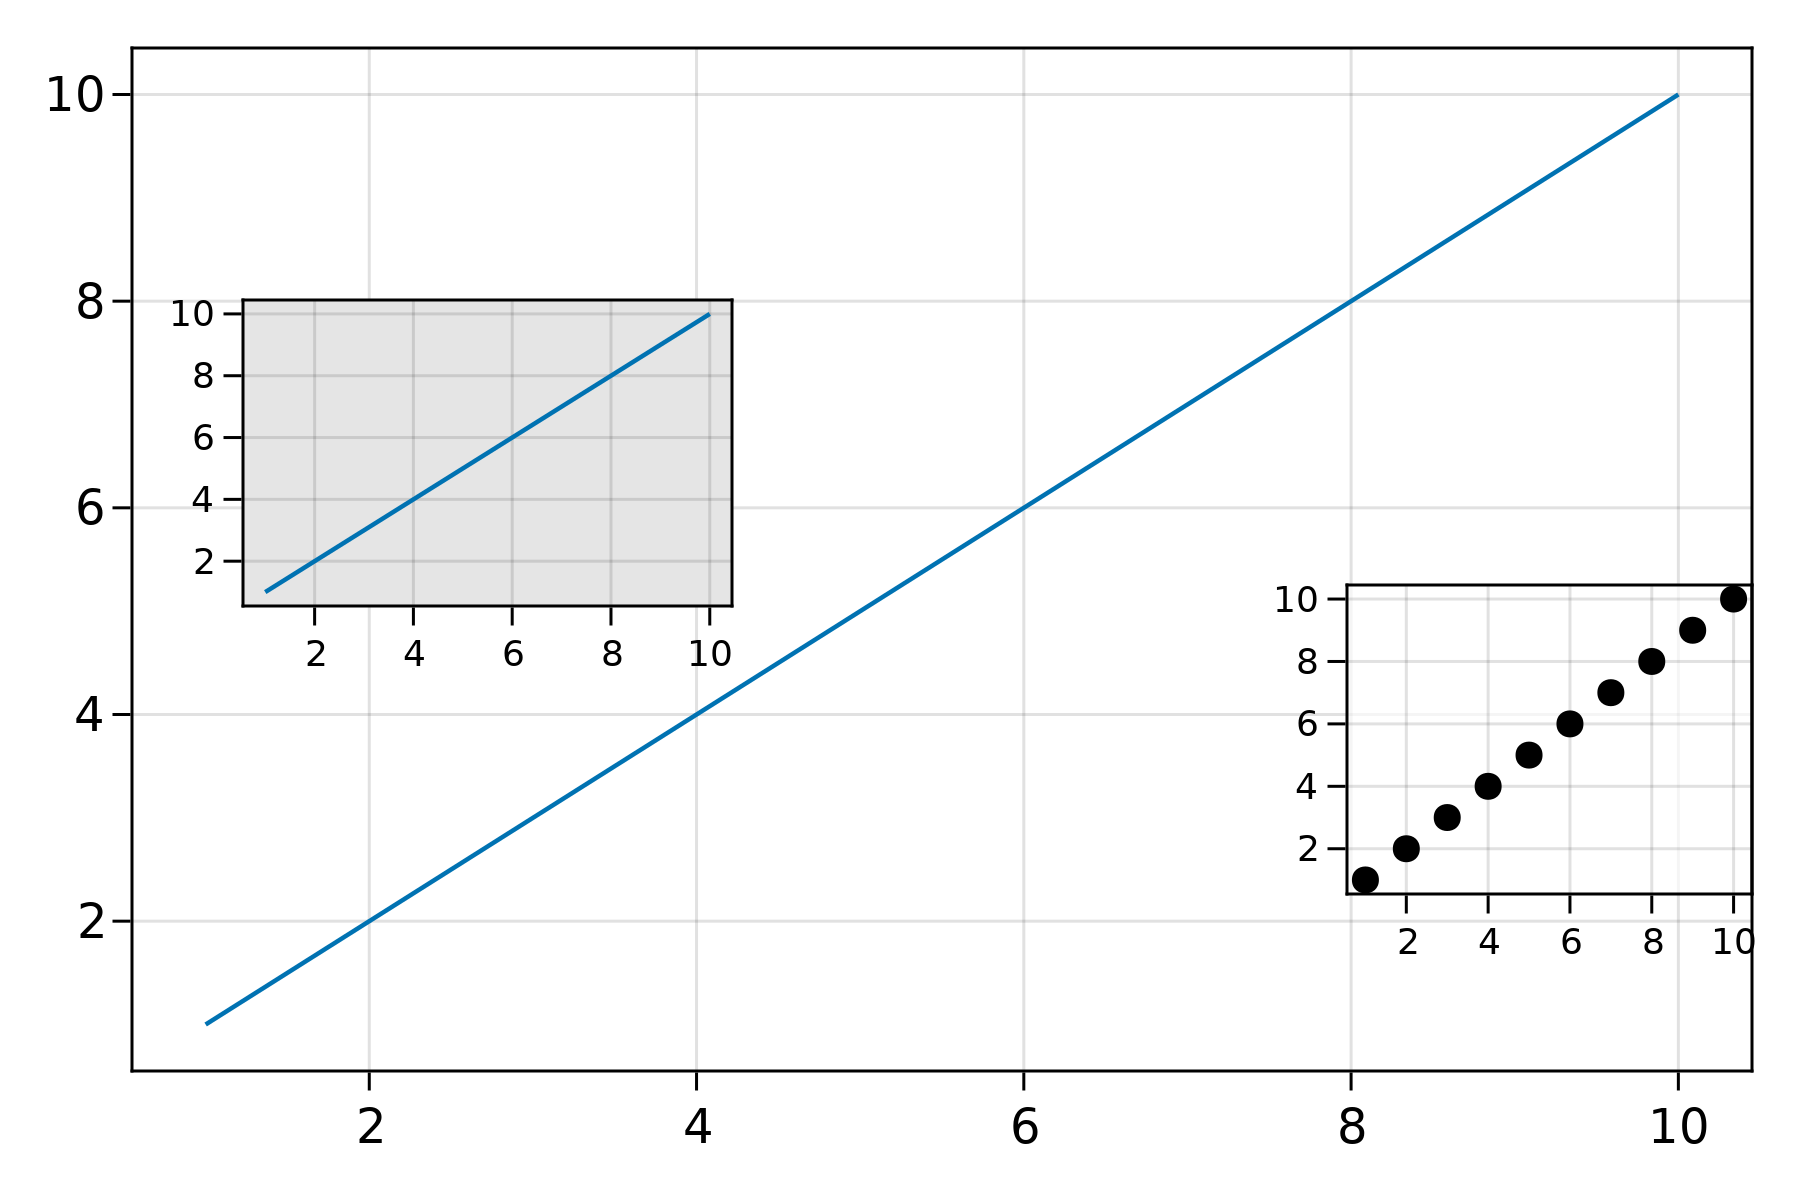
\includegraphics[width=0.6\textwidth,height=\textheight]{_build/im/JDS_figure_axis_inset_.png}
\caption{Figure axis inset.}\label{fig:figure_axis_inset}
}
\end{figure}

E isso deve cobrir os casos mais usados para layout com Makie. Agora,
vamos fazer alguns bons exemplos 3D com
\passthrough{\lstinline!GLMakie.jl!}.

\hypertarget{sec:glmakie}{%
\section{GLMakie.jl}\label{sec:glmakie}}

\passthrough{\lstinline!CairoMakie.jl!} fornece todas as nossas
necessidades de imagens 2D estáticas. Mas às vezes queremos
interatividade, principalmente quando estamos lidando com imagens 3D. A
visualização de dados em 3D também é uma prática comum para obter
insights de seus dados. É aqui que \passthrough{\lstinline!GLMakie.jl!}
pode ser útil, já que usa \href{http://www.opengl.org/}{OpenGL} como um
\emph{backend} que adiciona interatividade e capacidade de resposta a
\emph{plots}. Como antes, um \emph{plot} simples inclui, é claro, linhas
e pontos. Então, vamos começar com eles e como já sabemos como os
layouts funcionam, vamos colocar isso em prática.

\hypertarget{dispersuxe3o-e-linhas}{%
\subsection{Dispersão e Linhas}\label{dispersuxe3o-e-linhas}}

Para os gráficos de dispersão temos duas opções, a primeira é
\passthrough{\lstinline!scatter(x, y, z)!} e a segunda é
\passthrough{\lstinline!meshscatter(x, y, z)!}. Na primeira, os
marcadores não são escalonados nas direções dos eixos, mas na segunda,
porque são geometrias reais no espaço 3D. Veja o próximo exemplo:

\begin{lstlisting}
using GLMakie
GLMakie.activate!()
\end{lstlisting}

\begin{lstlisting}[language=Julia]
function scatters_in_3D()
    seed!(123)
    xyz = randn(10, 3)
    x, y, z = xyz[:, 1], xyz[:, 2], xyz[:, 3]
    fig = Figure(resolution=(1600, 400))
    ax1 = Axis3(fig[1, 1]; aspect=(1, 1, 1), perspectiveness=0.5)
    ax2 = Axis3(fig[1, 2]; aspect=(1, 1, 1), perspectiveness=0.5)
    ax3 = Axis3(fig[1, 3]; aspect=:data, perspectiveness=0.5)
    scatter!(ax1, x, y, z; markersize=50)
    meshscatter!(ax2, x, y, z; markersize=0.25)
    hm = meshscatter!(ax3, x, y, z; markersize=0.25,
        marker=FRect3D(Vec3f(0), Vec3f(1)), color=1:size(xyz)[2],
        colormap=:plasma, transparency=false)
    Colorbar(fig[1, 4], hm, label="values", height=Relative(0.5))
    fig
end
scatters_in_3D()
\end{lstlisting}

\begin{figure}
\hypertarget{fig:scatters_in_3D}{%
\centering
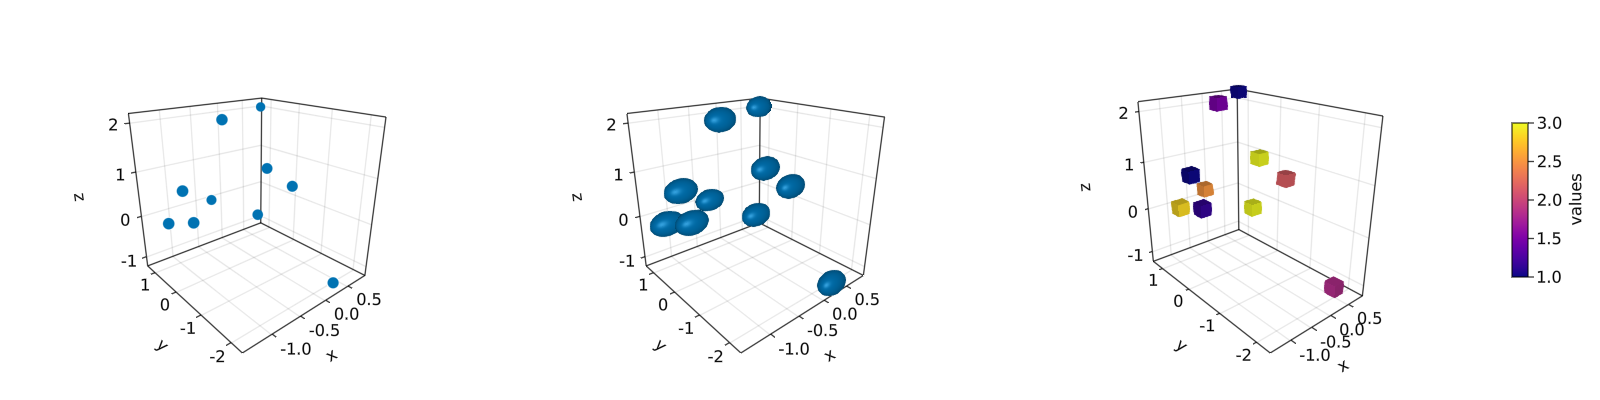
\includegraphics{_build/im/JDS_scatters_in_3D_.png}
\caption{Scatters in 3D.}\label{fig:scatters_in_3D}
}
\end{figure}

Observe também que uma geometria diferente pode ser passada como
marcadores, ou seja, um quadrado/ângulo e podemos atribuir-lhes uma
\passthrough{\lstinline!colormap!} também. No painel central, pode-se
obter esferas perfeitas fazendo \passthrough{\lstinline!aspect = :data!}
como no painel direito.

E fazendo \passthrough{\lstinline!lines!} ou
\passthrough{\lstinline!scatterlines!} é também bem simples:

\begin{lstlisting}[language=Julia]
function lines_in_3D()
    seed!(123)
    xyz = randn(10, 3)
    x, y, z = xyz[:, 1], xyz[:, 2], xyz[:, 3]
    fig = Figure(resolution=(1600, 400))
    ax1 = Axis3(fig[1, 1]; aspect=(1, 1, 1), perspectiveness=0.5)
    ax2 = Axis3(fig[1, 2]; aspect=(1, 1, 1), perspectiveness=0.5)
    ax3 = Axis3(fig[1, 3]; aspect=:data, perspectiveness=0.5)
    lines!(ax1, x, y, z; color=1:size(xyz)[2], linewidth=3)
    scatterlines!(ax2, x, y, z; markersize=50)
    hm = meshscatter!(ax3, x, y, z; markersize=0.2, color=1:size(xyz)[2])
    lines!(ax3, x, y, z; color=1:size(xyz)[2])
    Colorbar(fig[2, 1], hm; label="values", height=15, vertical=false,
        flipaxis=false, ticksize=15, tickalign=1, width=Relative(3.55 / 4))
    fig
end
lines_in_3D()
\end{lstlisting}

\begin{figure}
\hypertarget{fig:lines_in_3D}{%
\centering
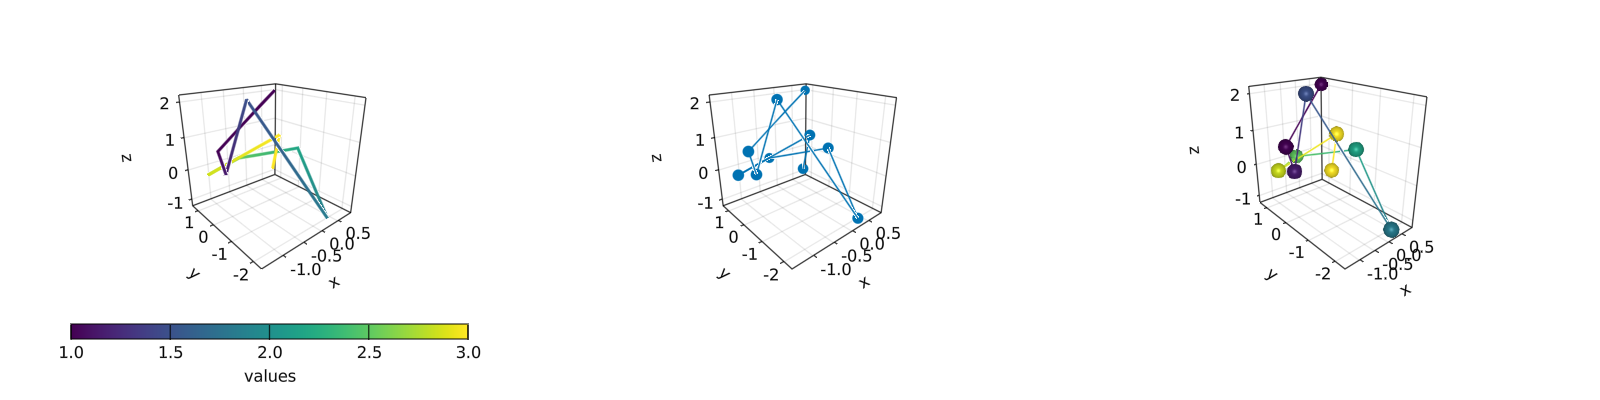
\includegraphics{_build/im/JDS_lines_in_3D_.png}
\caption{Lines in 3D.}\label{fig:lines_in_3D}
}
\end{figure}

Plotando uma \passthrough{\lstinline!surface!} também é fácil de ser
fazer assim como um \passthrough{\lstinline!wireframe!} e linhas
\passthrough{\lstinline!contour!} em 3D.

\hypertarget{surfaces-wireframe-contour-contourf-e-contour3d}{%
\subsection{\texorpdfstring{\texttt{surface}s, \texttt{wireframe},
\texttt{contour}, \texttt{contourf} e
\texttt{contour3d}}{surfaces, wireframe, contour, contourf e contour3d}}\label{surfaces-wireframe-contour-contourf-e-contour3d}}

Para mostrar estes casos, utilizaremos a seguinte função
\passthrough{\lstinline!peaks!}:

\begin{lstlisting}[language=Julia]
function peaks(; n=49)
    x = LinRange(-3, 3, n)
    y = LinRange(-3, 3, n)
    a = 3 * (1 .- x') .^ 2 .* exp.(-(x' .^ 2) .- (y .+ 1) .^ 2)
    b = 10 * (x' / 5 .- x' .^ 3 .- y .^ 5) .* exp.(-x' .^ 2 .- y .^ 2)
    c = 1 / 3 * exp.(-(x' .+ 1) .^ 2 .- y .^ 2)
    return (x, y, a .- b .- c)
end
\end{lstlisting}

A saída para as diferentes funções de plotagem é:

\begin{lstlisting}[language=Julia]
function plot_peaks_function()
    x, y, z = peaks()
    x2, y2, z2 = peaks(; n=15)
    fig = Figure(resolution=(1600, 400), fontsize=26)
    axs = [Axis3(fig[1, i]; aspect=(1, 1, 1)) for i = 1:3]
    hm = surface!(axs[1], x, y, z)
    wireframe!(axs[2], x2, y2, z2)
    contour3d!(axs[3], x, y, z; levels=20)
    Colorbar(fig[1, 4], hm, height=Relative(0.5))
    fig
end
plot_peaks_function()
\end{lstlisting}

\begin{figure}
\hypertarget{fig:plot_peaks_function}{%
\centering
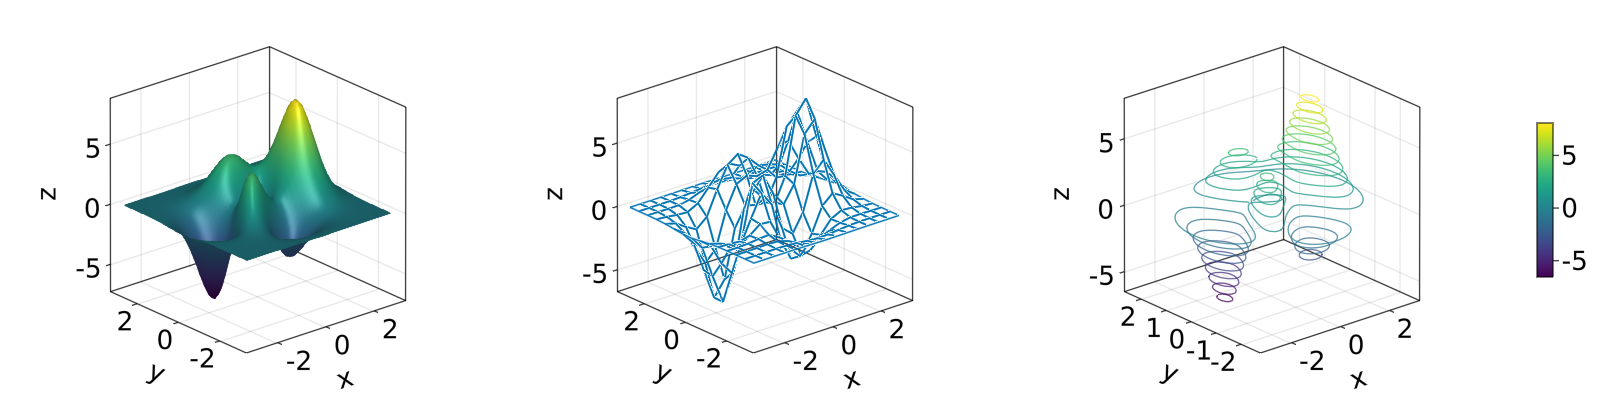
\includegraphics{_build/im/JDS_plot_peaks_function_.png}
\caption{Plot peaks function.}\label{fig:plot_peaks_function}
}
\end{figure}

Mas, também pode ser plotado com um
\passthrough{\lstinline!heatmap(x, y, z)!},
\passthrough{\lstinline!contour(x, y, z)!} ou
\passthrough{\lstinline!contourf(x, y, z)!}:

\begin{lstlisting}[language=Julia]
function heatmap_contour_and_contourf()
    x, y, z = peaks()
    fig = Figure(resolution=(1600, 400), fontsize=26)
    axs = [Axis(fig[1, i]; aspect=DataAspect()) for i = 1:3]
    hm = heatmap!(axs[1], x, y, z)
    contour!(axs[2], x, y, z; levels=20)
    contourf!(axs[3], x, y, z)
    Colorbar(fig[1, 4], hm, height=Relative(0.5))
    fig
end
heatmap_contour_and_contourf()
\end{lstlisting}

\begin{figure}
\hypertarget{fig:heatmap_contour_and_contourf}{%
\centering
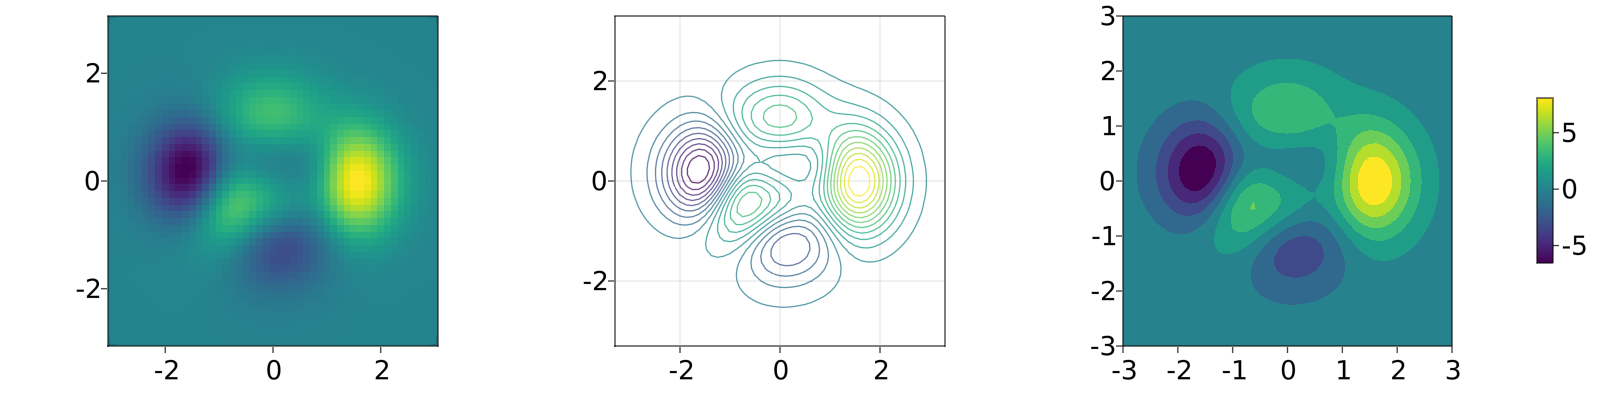
\includegraphics{_build/im/JDS_heatmap_contour_and_contourf_.png}
\caption{Heatmap contour and
contourf.}\label{fig:heatmap_contour_and_contourf}
}
\end{figure}

Adicionalmente, ao mudarmos \passthrough{\lstinline!Axis!} para um
\passthrough{\lstinline!Axis3!}, estes \emph{plots} estarão
automaticamente no plano x-y:

\begin{lstlisting}[language=Julia]
function heatmap_contour_and_contourf_in_a_3d_plane()
    x, y, z = peaks()
    fig = Figure(resolution=(1600, 400), fontsize=26)
    axs = [Axis3(fig[1, i]) for i = 1:3]
    hm = heatmap!(axs[1], x, y, z)
    contour!(axs[2], x, y, z; levels=20)
    contourf!(axs[3], x, y, z)
    Colorbar(fig[1, 4], hm, height=Relative(0.5))
    fig
end
heatmap_contour_and_contourf_in_a_3d_plane()
\end{lstlisting}

\begin{figure}
\hypertarget{fig:heatmap_contour_and_contourf_in_a_3d_plane}{%
\centering
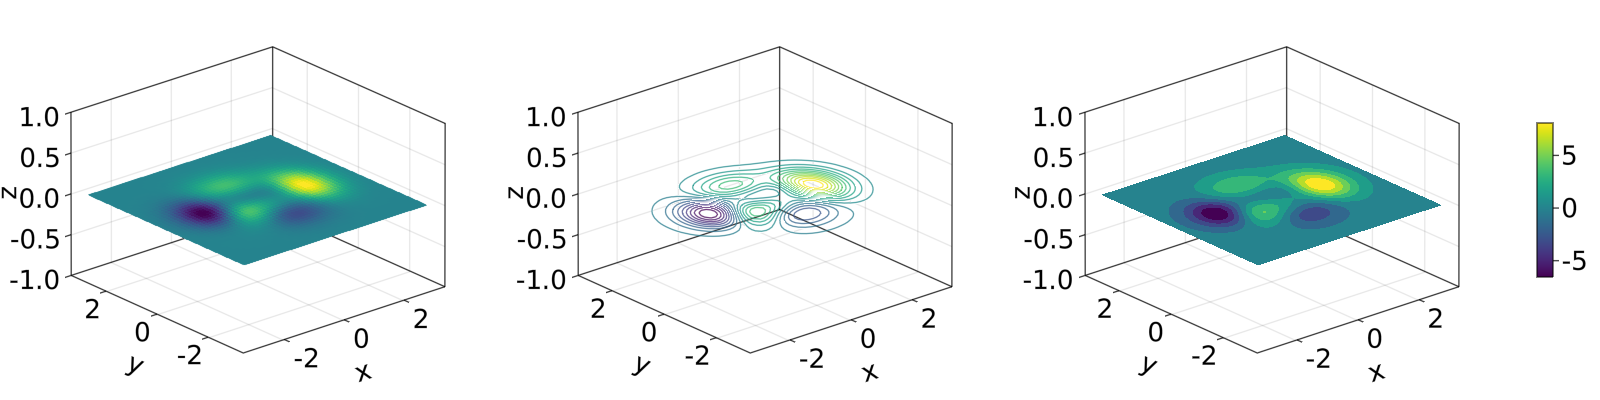
\includegraphics{_build/im/JDS_heatmap_contour_and_contourf_in_a_3d_plane_.png}
\caption{Heatmap contour and contourf in a 3d
plane.}\label{fig:heatmap_contour_and_contourf_in_a_3d_plane}
}
\end{figure}

Algo que também é bem facil de fazer é misturar todas essas fun;óes de
plotagens em um único \emph{plot}:

\begin{lstlisting}
using TestImages
\end{lstlisting}

\begin{lstlisting}[language=Julia]
function mixing_surface_contour3d_contour_and_contourf()
    img = testimage("coffee.png")
    x, y, z = peaks()
    cmap = :Spectral_11
    fig = Figure(resolution=(1200, 800), fontsize=26)
    ax1 = Axis3(fig[1, 1]; aspect=(1, 1, 1), elevation=pi / 6, xzpanelcolor=(:black, 0.75),
        perspectiveness=0.5, yzpanelcolor=:black, zgridcolor=:grey70,
        ygridcolor=:grey70, xgridcolor=:grey70)
    ax2 = Axis3(fig[1, 3]; aspect=(1, 1, 1), elevation=pi / 6, perspectiveness=0.5)
    hm = surface!(ax1, x, y, z; colormap=(cmap, 0.95), shading=true)
    contour3d!(ax1, x, y, z .+ 0.02; colormap=cmap, levels=20, linewidth=2)
    xmin, ymin, zmin = minimum(ax1.finallimits[])
    xmax, ymax, zmax = maximum(ax1.finallimits[])
    contour!(ax1, x, y, z; colormap=cmap, levels=20, transformation=(:xy, zmax))
    contourf!(ax1, x, y, z; colormap=cmap, transformation=(:xy, zmin))
    Colorbar(fig[1, 2], hm, width=15, ticksize=15, tickalign=1, height=Relative(0.35))
    # transformations into planes
    heatmap!(ax2, x, y, z; colormap=:viridis, transformation=(:yz, 3.5))
    contourf!(ax2, x, y, z; colormap=:CMRmap, transformation=(:xy, -3.5))
    contourf!(ax2, x, y, z; colormap=:bone_1, transformation=(:xz, 3.5))
    image!(ax2, -3 .. 3, -3 .. 2, rotr90(img); transformation=(:xy, 3.8))
    xlims!(ax2, -3.8, 3.8)
    ylims!(ax2, -3.8, 3.8)
    zlims!(ax2, -3.8, 3.8)
    fig
end
mixing_surface_contour3d_contour_and_contourf()
\end{lstlisting}

\begin{figure}
\hypertarget{fig:mixing_surface_contour3d_contour_and_contourf}{%
\centering
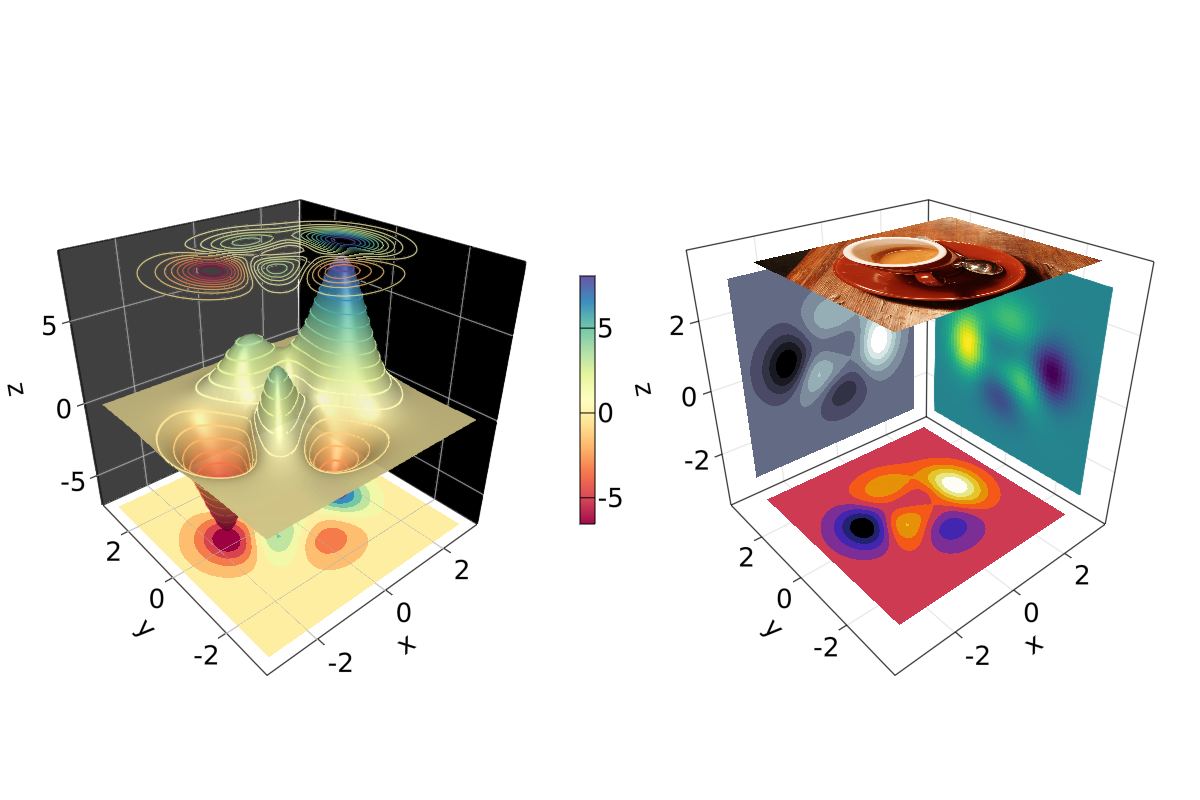
\includegraphics[width=0.6\textwidth,height=\textheight]{_build/im/JDS_mixing_surface_contour3d_contour_and_contourf_.png}
\caption{Mixing surface, contour3d, contour and
contourf.}\label{fig:mixing_surface_contour3d_contour_and_contourf}
}
\end{figure}

Não é ruim, certo? É claro que qualquer
\passthrough{\lstinline!heatmap!}s, \passthrough{\lstinline!contour!}s,
\passthrough{\lstinline!contourf!}s ou \passthrough{\lstinline!image!}
pode ser plotado em qualquer \emph{plot}.

\hypertarget{arrows-e-streamplots}{%
\subsection{\texorpdfstring{\texttt{arrows} e
\texttt{streamplots}}{arrows e streamplots}}\label{arrows-e-streamplots}}

\passthrough{\lstinline!arrows!} e \passthrough{\lstinline!streamplot!}
são \emph{plots} que podem ser úteis quando queremos saber as direções
que uma determinada variável seguirá. Veja uma demonstração
abaixo\footnote{Estamos usando o módulo
  \passthrough{\lstinline!LinearAlgebra!} da biblioteca padrão de Julia.}:

\begin{lstlisting}
using LinearAlgebra
\end{lstlisting}

\begin{lstlisting}[language=Julia]
function arrows_and_streamplot_in_3d()
    ps = [Point3f(x, y, z) for x = -3:1:3 for y = -3:1:3 for z = -3:1:3]
    ns = map(p -> 0.1 * rand() * Vec3f(p[2], p[3], p[1]), ps)
    lengths = norm.(ns)
    flowField(x, y, z) = Point(-y + x * (-1 + x^2 + y^2)^2, x + y * (-1 + x^2 + y^2)^2,
        z + x * (y - z^2))
    fig = Figure(resolution=(1200, 800), fontsize=26)
    axs = [Axis3(fig[1, i]; aspect=(1, 1, 1), perspectiveness=0.5) for i = 1:2]
    arrows!(axs[1], ps, ns, color=lengths, arrowsize=Vec3f0(0.2, 0.2, 0.3),
        linewidth=0.1)
    streamplot!(axs[2], flowField, -4 .. 4, -4 .. 4, -4 .. 4, colormap=:plasma,
        gridsize=(7, 7), arrow_size=0.25, linewidth=1)
    fig
end
arrows_and_streamplot_in_3d()
\end{lstlisting}

\begin{figure}
\hypertarget{fig:arrows_and_streamplot_in_3d}{%
\centering
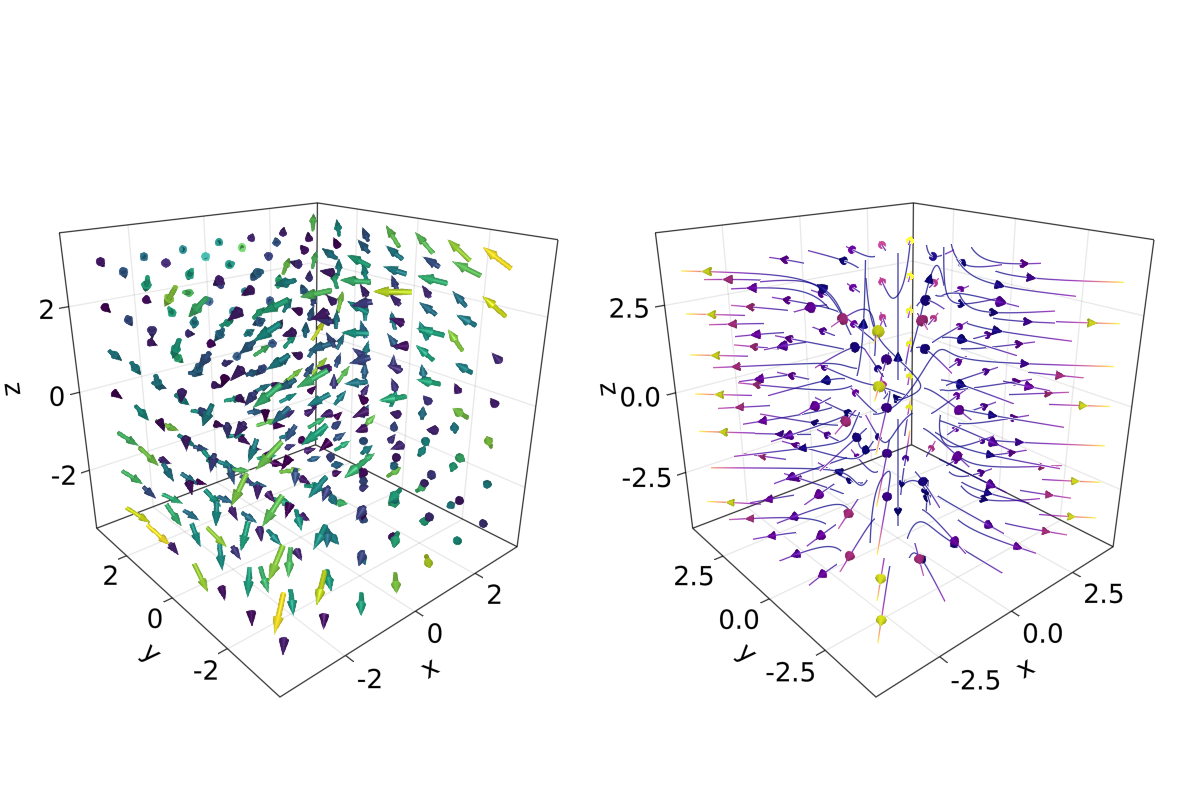
\includegraphics[width=0.6\textwidth,height=\textheight]{_build/im/JDS_arrows_and_streamplot_in_3d_.png}
\caption{Arrows and streamplot in
3d.}\label{fig:arrows_and_streamplot_in_3d}
}
\end{figure}

Outros exemplos interessantes são \passthrough{\lstinline!mesh(obj)!},
\passthrough{\lstinline!volume(x, y, z, vals)!}, e
\passthrough{\lstinline!contour(x, y, z, vals)!}.

\hypertarget{mesh-e-volumes}{%
\subsection{\texorpdfstring{\emph{Mesh} e
Volumes}{Mesh e Volumes}}\label{mesh-e-volumes}}

Visualizações de \emph{mesh} são úteis quando você quer plotar
geometrias, como uma \passthrough{\lstinline!Sphere!} ou um Retângulo,
ex: \passthrough{\lstinline!FRect3D!}. Outra abordagem para visualizar
pontos no espaço 3D é chamando as funções
\passthrough{\lstinline!volume!} e \passthrough{\lstinline!contour!},
que implementam
\href{https://en.wikipedia.org/wiki/Ray_tracing_(graphics)}{\emph{ray
tracing}} para simular uma grande variedade de efeitos ópticos. Veja os
próximos exemplos:

\begin{lstlisting}
using GeometryBasics
\end{lstlisting}

\begin{lstlisting}[language=Julia]
function mesh_volume_contour()
    # mesh objects
    rectMesh = FRect3D(Vec3f(-0.5), Vec3f(1))
    recmesh = GeometryBasics.mesh(rectMesh)
    sphere = Sphere(Point3f(0), 1)
    # https://juliageometry.github.io/GeometryBasics.jl/stable/primitives/
    spheremesh = GeometryBasics.mesh(Tesselation(sphere, 64))
    # uses 64 for tesselation, a smoother sphere
    colors = [rand() for v in recmesh.position]
    # cloud points for volume
    x = y = z = 1:10
    vals = randn(10, 10, 10)
    fig = Figure(resolution=(1600, 400))
    axs = [Axis3(fig[1, i]; aspect=(1, 1, 1), perspectiveness=0.5) for i = 1:3]
    mesh!(axs[1], recmesh; color=colors, colormap=:rainbow, shading=false)
    mesh!(axs[1], spheremesh; color=(:white, 0.25), transparency=true)
    volume!(axs[2], x, y, z, vals; colormap=Reverse(:plasma))
    contour!(axs[3], x, y, z, vals; colormap=Reverse(:plasma))
    fig
end
mesh_volume_contour()
\end{lstlisting}

\begin{figure}
\hypertarget{fig:mesh_volume_contour}{%
\centering
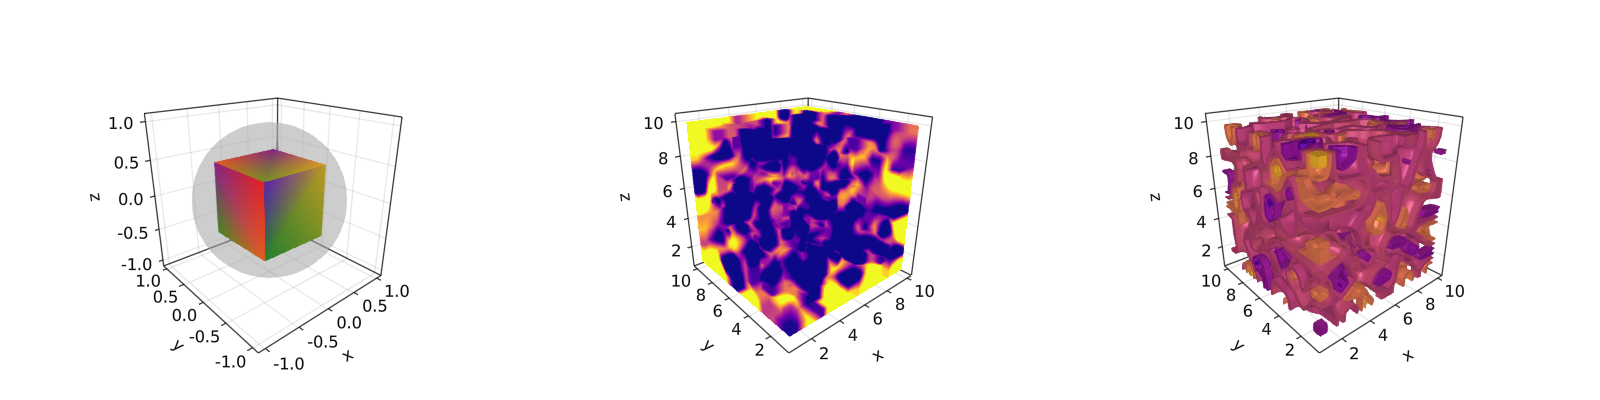
\includegraphics{_build/im/JDS_mesh_volume_contour_.png}
\caption{Mesh volume contour.}\label{fig:mesh_volume_contour}
}
\end{figure}

Note que aqui estamos traçando duas \emph{mesh} no mesmo eixo, uma
esfera transparente e um cubo. Até agora, cobrimos a maioria dos casos
de uso 3D. Outro exemplo é \passthrough{\lstinline!?linesegments!}.

Tomando como referência o exemplo anterior, pode-se fazer o seguinte
\emph{plot} personalizado com esferas e retângulos:

\begin{lstlisting}
using GeometryBasics, Colors
\end{lstlisting}

Para as esferas, vamos fazer um \emph{grid} retangular. Além disso,
usaremos uma cor diferente para cada uma delas. Adicionalmente, podemos
misturar esferas e um plano retangular. Em seguida, definimos todos os
dados necessários.

\begin{lstlisting}[language=Julia]
seed!(123)
spheresGrid = [Point3f(i,j,k) for i in 1:2:10 for j in 1:2:10 for k in 1:2:10]
colorSphere = [RGBA(i * 0.1, j * 0.1, k * 0.1, 0.75) for i in 1:2:10 for j in 1:2:10 for k in 1:2:10]
spheresPlane = [Point3f(i,j,k) for i in 1:2.5:20 for j in 1:2.5:10 for k in 1:2.5:4]
cmap = get(colorschemes[:plasma], LinRange(0, 1, 50))
colorsPlane = cmap[rand(1:50,50)]
rectMesh = FRect3D(Vec3f(-1, -1, 2.1), Vec3f(22, 11, 0.5))
recmesh = GeometryBasics.mesh(rectMesh)
colors = [RGBA(rand(4)...) for v in recmesh.position]
\end{lstlisting}

Então, o \emph{plot} é feito simplesmente com:

\begin{lstlisting}[language=Julia]
function grid_spheres_and_rectangle_as_plate()
    fig = with_theme(theme_dark()) do
        fig = Figure(resolution=(1200, 800))
        ax1 = Axis3(fig[1, 1]; aspect=:data, perspectiveness=0.5, azimuth=0.72)
        ax2 = Axis3(fig[1, 2]; aspect=:data, perspectiveness=0.5)
        meshscatter!(ax1, spheresGrid; color = colorSphere, markersize = 1,
            shading=false)
        meshscatter!(ax2, spheresPlane; color=colorsPlane, markersize = 0.75,
            lightposition=Vec3f(10, 5, 2), ambient=Vec3f(0.95, 0.95, 0.95),
            backlight=1.0f0)
        mesh!(recmesh; color=colors, colormap=:rainbow, shading=false)
        limits!(ax1, 0, 10, 0, 10, 0, 10)
        fig
    end
    fig
end
grid_spheres_and_rectangle_as_plate()
\end{lstlisting}

\begin{figure}
\hypertarget{fig:grid_spheres_and_rectangle_as_plate}{%
\centering
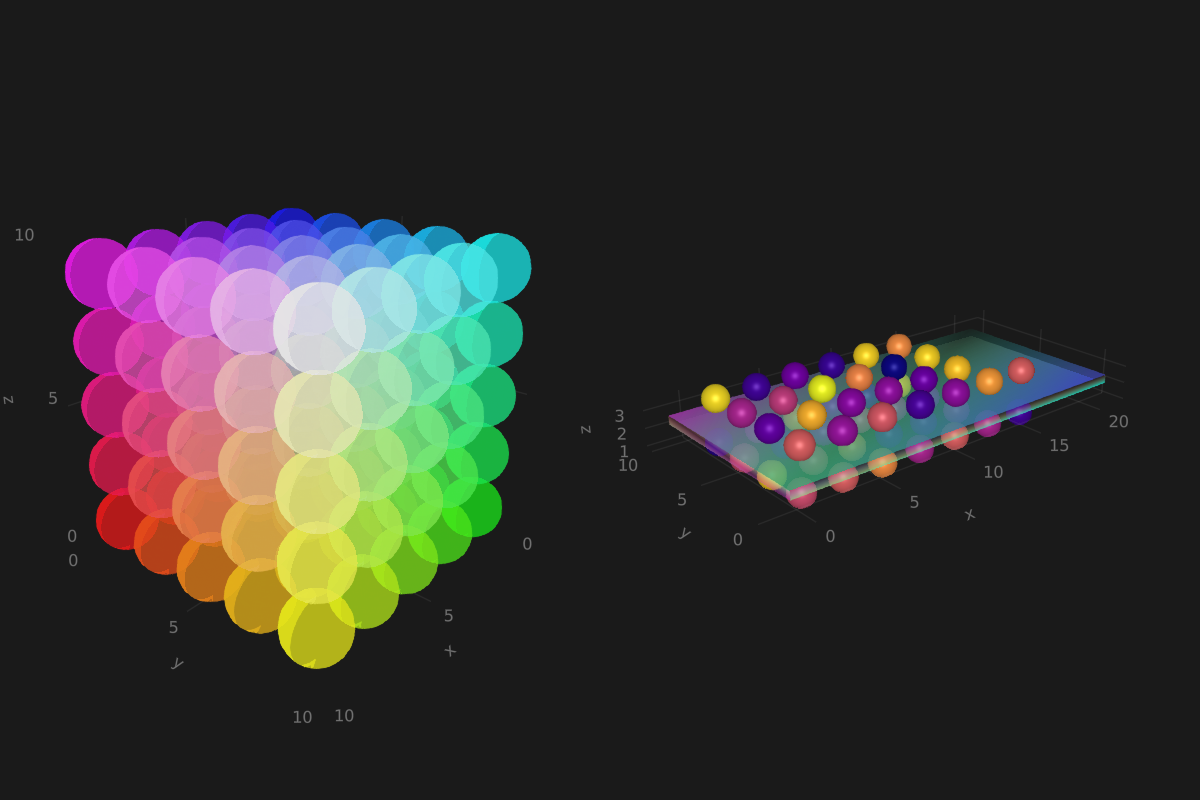
\includegraphics[width=0.6\textwidth,height=\textheight]{_build/im/JDS_grid_spheres_and_rectangle_as_plate_.png}
\caption{Grid spheres and rectangle as
plate.}\label{fig:grid_spheres_and_rectangle_as_plate}
}
\end{figure}

Aqui, o retângulo é semi-transparente devido ao canal alfa adicionado à
cor RGB. A função de retângulo é bastante versátil, por exemplo,
\emph{box} 3D é fácil implementar que por sua vez pode ser usada para
traçar um histograma 3D. Veja nosso próximo exemplo, onde estamos usando
novamente nossa função \passthrough{\lstinline!peaks!} e algumas
definições adicionais:

\begin{lstlisting}[language=Julia]
x, y, z = peaks(; n=15)
δx = (x[2] - x[1]) / 2
δy = (y[2] - y[1]) / 2
cbarPal = :Spectral_11
ztmp = (z .- minimum(z)) ./ (maximum(z .- minimum(z)))
cmap = get(colorschemes[cbarPal], ztmp)
cmap2 = reshape(cmap, size(z))
ztmp2 = abs.(z) ./ maximum(abs.(z)) .+ 0.15
\end{lstlisting}

aqui \(\delta x, \delta y\) são usados para especificar o tamanho das
\emph{box}. \passthrough{\lstinline!cmap2!} será a cor de cada
\emph{box} e \passthrough{\lstinline!ztmp2!} será usado como o parâmetro
de transparência. Veja o resultado na próxima figura.

\begin{lstlisting}[language=Julia]
function histogram_or_bars_in_3d()
    fig = Figure(resolution=(1200, 800), fontsize=26)
    ax1 = Axis3(fig[1, 1]; aspect=(1, 1, 1), elevation=π/6,
        perspectiveness=0.5)
    ax2 = Axis3(fig[1, 2]; aspect=(1, 1, 1), perspectiveness=0.5)
    rectMesh = FRect3D(Vec3f0(-0.5, -0.5, 0), Vec3f0(1, 1, 1))
    meshscatter!(ax1, x, y, 0*z, marker = rectMesh, color = z[:],
        markersize = Vec3f.(2δx, 2δy, z[:]), colormap = :Spectral_11,
        shading=false)
    limits!(ax1, -3.5, 3.5, -3.5, 3.5, -7.45, 7.45)
    meshscatter!(ax2, x, y, 0*z, marker = rectMesh, color = z[:],
        markersize = Vec3f.(2δx, 2δy, z[:]), colormap = (:Spectral_11, 0.25),
        shading=false, transparency=true)
    for (idx, i) in enumerate(x), (idy, j) in enumerate(y)
        rectMesh = FRect3D(Vec3f(i - δx, j - δy, 0), Vec3f(2δx, 2δy, z[idx, idy]))
        recmesh = GeometryBasics.mesh(rectMesh)
        lines!(ax2, recmesh; color=(cmap2[idx, idy], ztmp2[idx, idy]))
    end
    fig
end
histogram_or_bars_in_3d()
\end{lstlisting}

\begin{figure}
\hypertarget{fig:histogram_or_bars_in_3d}{%
\centering
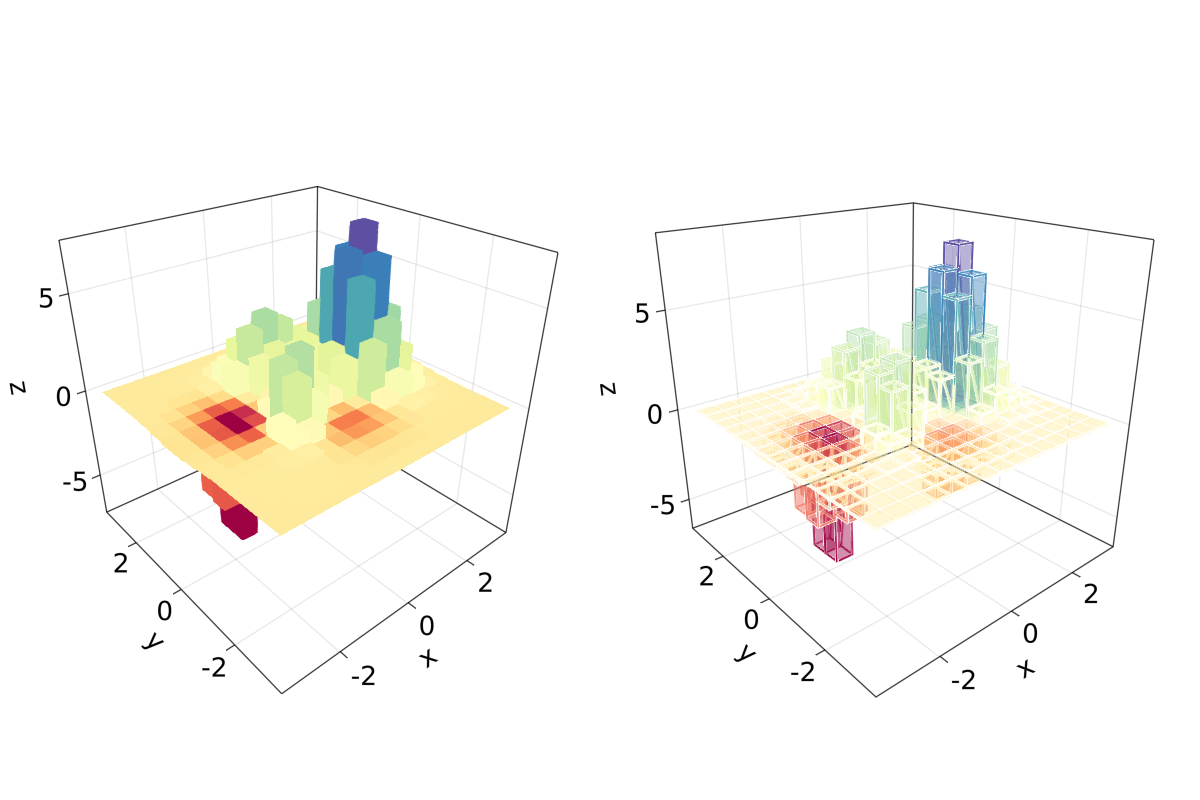
\includegraphics[width=0.6\textwidth,height=\textheight]{_build/im/JDS_histogram_or_bars_in_3d_.png}
\caption{Histogram or bars in 3d.}\label{fig:histogram_or_bars_in_3d}
}
\end{figure}

Note que você pode também usar \passthrough{\lstinline!lines!} ou
\passthrough{\lstinline!wireframe!} sobre um objeto \emph{mesh}.

\hypertarget{linhas-preenchidas-e-band}{%
\subsection{\texorpdfstring{Linhas Preenchidas e
\texttt{band}}{Linhas Preenchidas e band}}\label{linhas-preenchidas-e-band}}

Para o nosso último exemplo vamos mostrar como fazer uma curva
preenchida em 3d com \passthrough{\lstinline!band!} e alguns
\passthrough{\lstinline!linesegments!}:

\begin{lstlisting}[language=Julia]
function filled_line_and_linesegments_in_3D()
    xs = LinRange(-3, 3, 10)
    lower = [Point3f(i, -i, 0) for i in LinRange(0, 3, 100)]
    upper = [Point3f(i, -i, sin(i) * exp(-(i + i))) for i in range(0, 3, length=100)]
    fig = Figure(resolution=(1200, 800))
    axs = [Axis3(fig[1, i]; elevation=pi/6, perspectiveness=0.5) for i = 1:2]
    band!(axs[1], lower, upper, color=repeat(norm.(upper), outer=2), colormap=:CMRmap)
    lines!(axs[1], upper, color=:black)
    linesegments!(axs[2], cos.(xs), xs, sin.(xs), linewidth=5, color=1:length(xs))
    fig
end
filled_line_and_linesegments_in_3D()
\end{lstlisting}

\begin{figure}
\hypertarget{fig:filled_line_and_linesegments_in_3D}{%
\centering
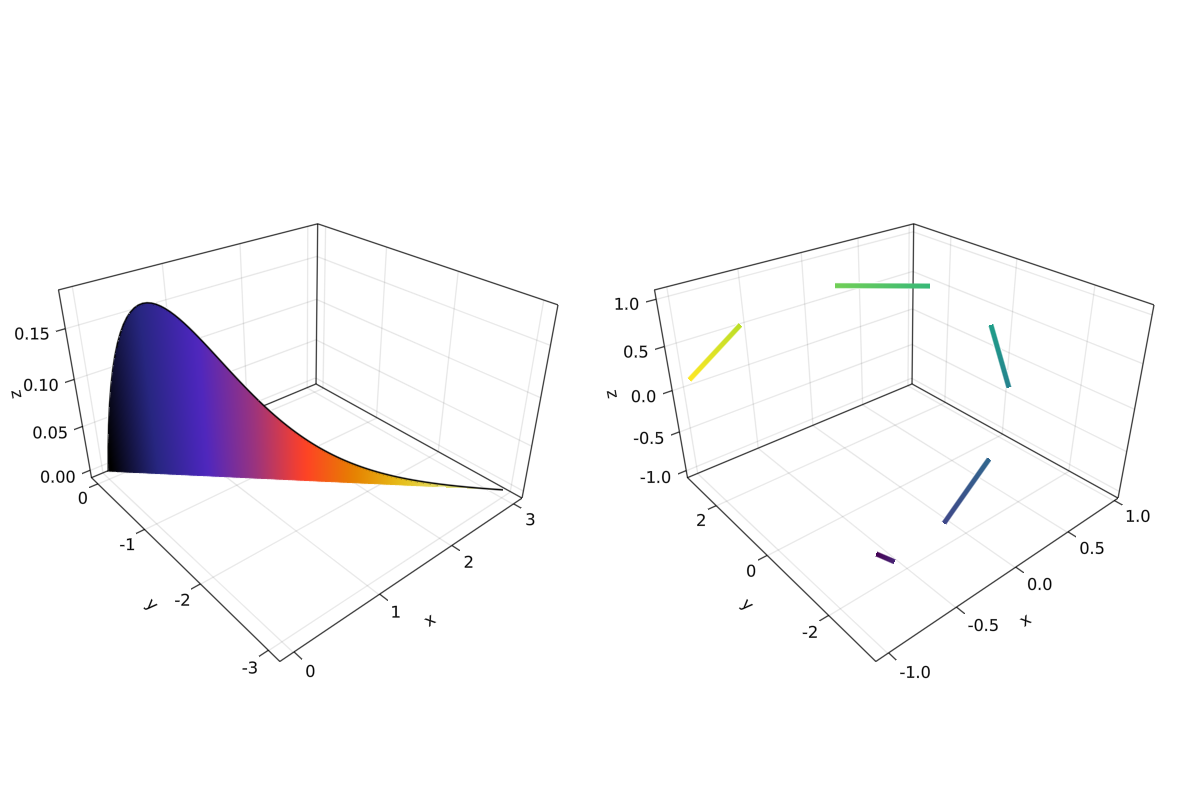
\includegraphics[width=0.6\textwidth,height=\textheight]{_build/im/JDS_filled_line_and_linesegments_in_3D_.png}
\caption{Filled line and linesegments in
3D.}\label{fig:filled_line_and_linesegments_in_3D}
}
\end{figure}

Finalmente, nossa jornada fazendo \emph{plots} 3D chegou ao fim. Você
pode combinar tudo o que expostos aqui para criar imagens 3D incríveis!

\hypertarget{sec:appendix}{%
\chapter{Apêndice}\label{sec:appendix}}

\hypertarget{sec:appendix_pkg}{%
\section{Versões dos Pacotes}\label{sec:appendix_pkg}}

Esse livro foi feito com Julia 1.7.3 e os seguintes pacotes:

\begin{lstlisting}[language=Julia]
Books 1.2.8
CSV 0.10.8
CairoMakie 0.7.5
CategoricalArrays 0.10.7
ColorSchemes 3.20.0
Colors 0.12.8
DataFrames 1.4.4
Distributions 0.25.79
FileIO 1.16.0
GLMakie 0.5.5
GeometryBasics 0.4.5
ImageMagick 1.2.2
LaTeXStrings 1.3.0
Makie 0.16.6
QuartzImageIO 0.7.4
Reexport 1.2.2
StatsBase 0.33.21
TestImages 1.7.1
XLSX 0.7.10
\end{lstlisting}

Build: 2022-12-11 21:5 UTC

\hypertarget{sec:notation}{%
\section{Formatação}\label{sec:notation}}

Neste livro, nós tentamos manter a formatação de código-fonte o mais
consistente possível. Isto permite uma melhor leitura e escrita de
código-fonte. Definimos o padrão de formatação em três partes.

\hypertarget{julia-style-guide}{%
\subsection{Julia Style Guide}\label{julia-style-guide}}

Primeiramente, nós tentamos aderir as convenções do
\href{https://docs.julialang.org/en/v1/manual/style-guide/}{Julia Style
Guide}. Mais importante, escrevemos funções e não scripts (veja também
Section~\ref{sec:engineering}). Além disso, usamos convenções de
nomenclatura consistente com o módulo \passthrough{\lstinline!base!} de
Julia:

\begin{itemize}
\tightlist
\item
  Uso de \emph{camelcase} para módulos:
  \passthrough{\lstinline!module JuliaDataScience!},
  \passthrough{\lstinline!struct MyPoint!}. (Note que a denominação de
  \emph{camelcase} é porque a capitalização das palavras, tais como
  ``iPad'' ou ``CamelCase,'' faz com que a palavra se assemelhe que nem
  as costas de um camelo.)
\item
  Denominação de funções usando caixa baixa (\emph{lowercase}) e
  separando palavras por \emph{underline}
  (\passthrough{\lstinline!\_!}). Também é permitido omitir o separador
  quando nomeando funções. Por exemplo, estes nomes de funções são
  consistentes com as convenções:
  \passthrough{\lstinline!my\_function!},
  \passthrough{\lstinline!myfunction!} e
  \passthrough{\lstinline!string2int!}.
\end{itemize}

Adicionalmente, evitamos usar parênteses em condicionais, ou seja,
escrevemos \passthrough{\lstinline!if a == b!} ao invés de
\passthrough{\lstinline!if (a == b)!} e usamos 4 espaços para cada nível
de indentação.

\hypertarget{bluestyle}{%
\subsection{BlueStyle}\label{bluestyle}}

O \href{https://github.com/invenia/BlueStyle}{Blue Style Guide} adiciona
diversas convenções aos padrões do Guia de Estilo de Julia. Algumas
dessas regras podem soar pedantes, mas descobrimos que elas fazem o
código ficar mais legível.

Do Blue Style Guide, nós aderimos especificamente à:

\begin{itemize}
\item
  No máximo 92 caracteres por linha em código-fonte (para arquivos
  Markdown, linhas mais longas são permitidas).
\item
  Quando carregando código com \passthrough{\lstinline!using!}, usar
  apenas uma declaração por módulo por linha.
\item
  Não há whitespace no fim das linhas. Whitespace no fim das linhas faz
  com que a inspeção do código seja mais difícil pois eles não mudam o
  comportamento do código mas podem ser interpretados como mudanças.
\item
  Evitar espacos adicionais dentro dos parênteses. Escreva
  \passthrough{\lstinline!string(1, 2)!} ao invés de
  \passthrough{\lstinline!string( 1 , 2 )!}.
\item
  Variávies globais devem ser evitadas.
\item
  Tente limitar nomes de funções para apenas uma ou duas palavras.
\item
  Use o ponto-e-virgula para distinção se um argumento é posicional ou
  de palavra-chave. Por exemplo, \passthrough{\lstinline!func(x; y=3)!}
  ao invés de \passthrough{\lstinline!func(x, y=3)!}.
\item
  Evite usar espaços múltiplos para alinhar coisas. Escreva

\begin{lstlisting}
a = 1
lorem = 2
\end{lstlisting}

  ao invés de

\begin{lstlisting}
a     = 1
lorem = 2
\end{lstlisting}
\item
  Sempre que apropriado, coloque espaços ao redor de operadores
  binários, por exemplo, \passthrough{\lstinline!1 == 2!} ou
  \passthrough{\lstinline!y = x + 1!}.
\item
  Indente quotações triplas:

\begin{lstlisting}
s = """
    my long text:
    [...]
    the end.
    """
\end{lstlisting}
\item
  Não omite zeros in floats (mesmo que Julia permita). Portanto, escreva
  \passthrough{\lstinline!1.0!} ao invés de \passthrough{\lstinline!1.!}
  e escreva \passthrough{\lstinline!0.1!} ao invés de
  \passthrough{\lstinline!.1!}.
\item
  Use \passthrough{\lstinline!in!} dentro de loops for e não = ou ∈
  (mesmo que Julia permita).
\end{itemize}

\hypertarget{nossos-incrementos-ao-blue-style-guide}{%
\subsection{Nossos incrementos ao Blue Style
Guide}\label{nossos-incrementos-ao-blue-style-guide}}

\begin{itemize}
\tightlist
\item
  No texto, referenciamos uma chamada de função
  \passthrough{\lstinline!M.foo(3, 4)!} como
  \passthrough{\lstinline!M.foo!} e não
  \passthrough{\lstinline!M.foo(...)!} ou
  \passthrough{\lstinline!M.foo()!}.
\item
  Quando falando sobre pacotes, tais como o pacote DataFrames, nós
  explicitamente escrevemos sempre
  \passthrough{\lstinline!DataFrames.jl!}. Isto faz com que seja fácil
  reconhecer que estamos nos referindo à um pacote.
\item
  Para nome de arquivos, mantemos a notação como ``file.txt'' e não
  \passthrough{\lstinline!file.txt!} ou file.txt, pois é consistente com
  o código-fonte.
\item
  Para nomes e colunas em tabelas, tais como a coluna
  \passthrough{\lstinline!x!}, usamos a coluna
  \passthrough{\lstinline!:x!}, porque é consistente com o código-fonte.
\item
  Não usamos símbolos Unicode fora dos blocos de código. Isto foi
  necessário por conta de um bug na geração do PDF.
\item
  A linha antes de cada código de bloco termina com dois pontos (:) para
  indicar que aquela linha pertence aquele bloco de código.
\end{itemize}

\hypertarget{carregamento-de-suxedmbolos}{%
\subsubsection{Carregamento de
símbolos}\label{carregamento-de-suxedmbolos}}

Prefira sempre carregar símbolos de maneira explícita, ou seja, prefira
\passthrough{\lstinline!using A: foo!} ao invés de
\passthrough{\lstinline!using A!} quando não estiver usando o REPL (veja
também \protect\hyperlink{ref-jump2021using}{\emph{JuMP Style Guide},
2021}). Neste contexto, um símbolo significa um identificado de um
objeto. Por exemplo, mesmo que não parece natural, internamente
\passthrough{\lstinline!DataFrame!}, \passthrough{\lstinline!π!} e
\passthrough{\lstinline!CSV!} são todos símbolos. Podemos averiguar isto
se usarmos uma função introspectiva de Julia tal como
\passthrough{\lstinline!isdefined!}:

\begin{lstlisting}[language=Julia]
isdefined(Main, :π)
\end{lstlisting}

\begin{lstlisting}[language=Output]
true
\end{lstlisting}

Adjacente de ser explícito no uso de \passthrough{\lstinline!using!},
prefira também \passthrough{\lstinline!using A: foo!} ao invẽs de
\passthrough{\lstinline!import A: foo!} porque este último faz com que
seja fácil estender acidentalmente \passthrough{\lstinline!foo!}. Note
que isto não é somente aplicável para Julia: carregament implícito de
símbolos por \passthrough{\lstinline!from <module> import *!} também é
desencorajado em Python (\protect\hyperlink{ref-pep8}{van Rossum et al.,
2001}).

A razão da importância de ser explícito está relacionada com
versionamento semântico. Com versionamento semântico
(\url{http://semver.org}), o número da versão está relacionado se um
pacote possui ou não mudanças \emph{breaking}. Por exemplo, uma mudança
\emph{non-breaking} que atualiza o pacote \passthrough{\lstinline!A!} se
dá quando o pacote migra da versão \passthrough{\lstinline!0.2.2!} para
\passthrough{\lstinline!0.2.3!}. Com tais mudanças \emph{non-breaking},
você não precisa se preocupar se o seu pacote vai quebrar
(\emph{break}), em outras palavras, dar um erro ou mudar o comportamento
de execução. Se um pacote \passthrough{\lstinline!A!} migra de versão
\passthrough{\lstinline!0.2!} para \passthrough{\lstinline!1.0!}, então
esta atualização é \emph{breaking} e você provavelmente terá que fazer
mudanças no seu código para fazer com que o pacote
\passthrough{\lstinline!A!} funcione novamente. \textbf{Porém},
exportando símbolos extras é considerado uma mudança
\emph{non-breaking}. Então, com carreamento implícito de símbolos
\textbf{mudanças \emph{non-breaking} podem quebrar seu pacote}. Por isso
que é uma boa prática apeans carregar símbolos de maneira explícita.

\hypertarget{referuxeancias}{%
\chapter*{Referências}\label{referuxeancias}}
\addcontentsline{toc}{chapter}{Referências}

\hypertarget{refs}{}
\begin{CSLReferences}{1}{0}
\leavevmode\hypertarget{ref-bezanson2017julia}{}%
Bezanson, J., Edelman, A., Karpinski, S., \& Shah, V. B. (2017). Julia:
{A} fresh approach to numerical computing. \emph{SIAM Review},
\emph{59}(1), 65--98.

\leavevmode\hypertarget{ref-chen2014big}{}%
Chen, M., Mao, S., \& Liu, Y. (2014). Big data: A survey. \emph{Mobile
Networks and Applications}, \emph{19}(2), 171--209.

\leavevmode\hypertarget{ref-domo2018data}{}%
Domo. (2018). \emph{Data never sleeps 6.0}.
\url{https://www.domo.com/assets/downloads/18_domo_data-never-sleeps-6+verticals.pdf}

\leavevmode\hypertarget{ref-fitzgerald2020idc}{}%
Fitzgerald, S., Jimenez, D. Z., S., F., Yorifuji, Y., Kumar, M., Wu, L.,
Carosella, G., Ng, S., Parker, P., R. Carter, \& Whalen, M. (2020). IDC
FutureScape: Worldwide digital transformation 2021 predictions.
\emph{IDC FutureScape}.

\leavevmode\hypertarget{ref-gantz2012digital}{}%
Gantz, J., \& Reinsel, D. (2012). The digital universe in 2020: Big
data, bigger digital shadows, and biggest growth in the far east.
\emph{IDC iView: IDC Analyze the Future}, \emph{2007}(2012), 1--16.

\leavevmode\hypertarget{ref-jump2021using}{}%
\emph{JuMP style guide}. (2021).
\url{https://jump.dev/JuMP.jl/v0.21/developers/style/\#using-vs.-import}

\leavevmode\hypertarget{ref-khan2014big}{}%
Khan, N., Yaqoob, I., Hashem, I. A. T., Inayat, Z., Mahmoud Ali, W. K.,
Alam, M., Shiraz, M., \& Gani, A. (2014). Big data: Survey,
technologies, opportunities, and challenges. \emph{The Scientific World
Journal}, \emph{2014}.

\leavevmode\hypertarget{ref-Meng2019Data}{}%
Meng, X.-L. (2019). Data science: An artificial ecosystem. \emph{Harvard
Data Science Review}, \emph{1}(1).
\url{https://doi.org/10.1162/99608f92.ba20f892}

\leavevmode\hypertarget{ref-perkelJuliaComeSyntax2019}{}%
Perkel, J. M. (2019). Julia: Come for the syntax, stay for the speed.
\emph{Nature}, \emph{572}(7767), 141--142.
\url{https://doi.org/10.1038/d41586-019-02310-3}

\leavevmode\hypertarget{ref-storopoli2021bayesianjulia}{}%
Storopoli, J. (2021). \emph{Bayesian statistics with julia and turing}.
\url{https://storopoli.io/Bayesian-Julia}

\leavevmode\hypertarget{ref-tanmaybakshiBakingKnowledgeMachine2021}{}%
tanmay bakshi. (2021). \emph{Baking {Knowledge} into {Machine Learning
Models}{{Chris Rackauckas}} on {TechLifeSkills} w/ {Tanmay Ep}.55}.
\url{https://youtu.be/moyPIhvw4Nk}

\leavevmode\hypertarget{ref-tedxtalksProgrammingLanguageHeal2020}{}%
TEDx Talks. (2020). \emph{A programming language to heal the planet
together: {Julia} \textbar{} {Alan Edelman} \textbar{} {TEDxMIT}}.
\url{https://youtu.be/qGW0GT1rCvs}

\leavevmode\hypertarget{ref-pep8}{}%
van Rossum, G., Warsaw, B., \& Coghlan, N. (2001). \emph{Style guide for
{Python} code} (PEP No. 8).
\url{https://www.python.org/dev/peps/pep-0008/}

\leavevmode\hypertarget{ref-wickham2011split}{}%
Wickham, H. (2011). The split-apply-combine strategy for data analysis.
\emph{Journal of Statistical Software}, \emph{40}(1), 1--29.

\end{CSLReferences}

\backmatter

\end{document}
